\documentclass{disithesis}
\usepackage[utf8]{inputenc}
% \usepackage{amsmath}
% \usepackage{bm}
\usepackage{graphicx}

% \usepackage[allfiguresdraft]{draftfigure} % SWITCH OFF FIGURES

\usepackage{multirow}
\usepackage{times}
\usepackage{epsfig}
\usepackage{amsmath}
\usepackage{amssymb}
\usepackage{rotating}
\usepackage{pdflscape}
%DIF PREAMBLE EXTENSION ADDED BY LATEXDIFF
%DIF UNDERLINE PREAMBLE %DIF PREAMBLE
\RequirePackage[normalem]{ulem} %DIF PREAMBLE
\RequirePackage{color}\definecolor{RED}{rgb}{1,0,0}\definecolor{BLUE}{rgb}{0,0,1} %DIF PREAMBLE
\providecommand{\DIFadd}[1]{{\protect\color{blue}\uwave{#1}}} %DIF PREAMBLE
\providecommand{\DIFdel}[1]{{\protect\color{red}\sout{#1}}}                      %DIF PREAMBLE
%DIF SAFE PREAMBLE %DIF PREAMBLE
\providecommand{\DIFaddbegin}{} %DIF PREAMBLE
\providecommand{\DIFaddend}{} %DIF PREAMBLE
\providecommand{\DIFdelbegin}{} %DIF PREAMBLE
\providecommand{\DIFdelend}{} %DIF PREAMBLE
%DIF FLOATSAFE PREAMBLE %DIF PREAMBLE
\providecommand{\DIFaddFL}[1]{\DIFadd{#1}} %DIF PREAMBLE
\providecommand{\DIFdelFL}[1]{\DIFdel{#1}} %DIF PREAMBLE
\providecommand{\DIFaddbeginFL}{} %DIF PREAMBLE
\providecommand{\DIFaddendFL}{} %DIF PREAMBLE
\providecommand{\DIFdelbeginFL}{} %DIF PREAMBLE
\providecommand{\DIFdelendFL}{} %DIF PREAMBLE
%DIF END PREAMBLE EXTENSION ADDED BY LATEXDIFF

% !TEX root = ./main.tex

% Abbreviations
\usepackage{xspace}
\newcommand*{\eg}{e.g.\@\xspace}
\newcommand*{\ie}{i.e.\@\xspace}
\newcommand*{\ade}{{\sc adenine}\@\xspace}

% MS stuff
\newcommand*{\RR}{{\em RR}\@\xspace}
\newcommand*{\SP}{{\em SP}\@\xspace}
\newcommand*{\PP}{{\em PP}\@\xspace}
\newcommand*{\PR}{{\em PR}\@\xspace}
\newcommand*{\CIS}{{\em CIS}\@\xspace}
\newcommand*{\PCOs}{{PCOs}\@\xspace}
\newcommand*{\PCO}{{\em PCO}\@\xspace}

% GENE SYMBOL
\newcommand{\apc}{{\sc apc}\@\xspace}
\newcommand{\kras}{{\sc kras}\@\xspace}
\newcommand{\ctnnb}{{\sc ctnnb{\footnotesize 1}}\@\xspace}
\newcommand{\tp}{{\sc tp{\footnotesize 53}}\@\xspace}
\newcommand{\msh}{{\sc msh{\footnotesize 2}}\@\xspace}
\newcommand{\mlh}{{\sc mlh{\footnotesize 1}}\@\xspace}
\newcommand{\pms}{{\sc pms{\footnotesize 2}}\@\xspace}
\newcommand{\pten}{{\sc pten}\@\xspace}
\newcommand{\smad}{{\sc smad{\footnotesize 4}}\@\xspace}
\newcommand{\stk}{{\sc stk{\footnotesize 11}}\@\xspace}
\newcommand{\gsk}{{\sc gsk{\footnotesize 3}b}\@\xspace}
\newcommand{\axin}{{\sc axin{\footnotesize 2}}\@\xspace}


% Math stuff
\usepackage{amsmath,amsfonts,dsfont,mathrsfs,mathtools,amssymb}
\usepackage{bm}
\newcommand{\dataset}{{\cal D}}
\newcommand{\fracpartial}[2]{\frac{\partial #1}{\partial  #2}}
\newcommand{\argmin}[1]{\underset{#1}{\operatorname{arg}\,\operatorname{min}}\;}
\newcommand{\argmax}[1]{\underset{#1}{\operatorname{arg}\,\operatorname{max}}\;}
\newcommand{\norm}[1]{\left\lVert#1\right\rVert}

% Notes
\usepackage{xcolor}
\newcommand\todo[1]{\textcolor{red}{{\bf \{#1\}}}} %TODO
\newcommand{\me}[0]{Samuele Fiorini}
%\newcommand{\longtitle}[0]{Understanding time-evolving \\ biomedical data with machine learning}
%\newcommand{\longtitle}[0]{From biological questions to ...\\ }
\newcommand{\longtitle}[0]{Challenges in biomedical data science:\\data-driven solutions to clinical questions}
\newcommand{\runningtitle}[0]{Machine Learning 4 healthcare}

% Code snippets and quotations
\usepackage{listings}
\usepackage{csquotes}
\usepackage{algorithm, algpseudocode}


% Images root
\graphicspath{{../images/}}

% Additional handy packages
\usepackage[T1]{fontenc}
\usepackage[english]{babel}
\usepackage{booktabs}
\usepackage[inline]{enumitem}
\usepackage{caption}
% \usepackage{subcaption}
\usepackage{longtable}
\usepackage{graphicx}
\usepackage{subfig}
\usepackage{tikz}
\usetikzlibrary{automata,arrows,positioning,calc}


% %% Edit the Part appearance
\usepackage{xpatch}
\makeatletter
\xpatchcmd{\@part}{\huge\bfseries \partname\nobreakspace\thepart}{}{}{}
\makeatother


% biblio
\usepackage{natbib}
\renewcommand\cite{\citep}
\setcitestyle{square}

% ---------- Corradi stuff ------------------ %
\usepackage{titlesec}
\usepackage{imakeidx}
\usepackage{microtype}
\usepackage{currfile}

% For really empty page before chapter
\let\origdoublepage\cleardoublepage
\newcommand{\clearemptydoublepage}{%
  \clearpage
  {\pagestyle{empty}\origdoublepage}%
}
\let\cleardoublepage\clearemptydoublepage

\renewcommand{\chaptername}{}

\titleformat{\chapter}
  {\normalfont\LARGE\bfseries}{\thechapter}{1em}{}
\titlespacing*{\chapter}{0pt}{3.5ex plus 1ex minus .2ex}{2.3ex plus .2ex}

\usepackage{ifpdf}

\usepackage[pdftex,pagebackref,hidelinks]{hyperref}

% hyperref backref
\renewcommand*{\backref}[1]{}
\renewcommand*{\backrefalt}[4]{[{\footnotesize%
\ifcase #1 Not cited.%
\or Cited on page~#2.%
\else Cited on pages #2.%
\fi%
}]}
% ---------- end Corradi stuff ------------------ %


% url appeareance
% \usepackage{url}
\usepackage{breakurl}
\DeclareUrlCommand\ULurl{%
  \renewcommand\UrlFont{\small\ttfamily\color{blue}}%
  \renewcommand\UrlLeft{\uline\bgroup}%
  \renewcommand\UrlRight{\egroup}}

\renewcommand\url[1]{\href{#1}{\ULurl{#1}}}



\begin{document}
\title{\longtitle}

\author{\me}

%%%% If month and year are not the current ones
%%%% \submityear{1997}
%%%% \submitmonth{December}

\technumber{XX}

\maketitle

\begin{addresspage}
{\bf
Dottorato di Ricerca in Informatica ed Ingegneria dei Sistemi\\
Indirizzo Informatica\\
Dipartimento di Informatica, Bioingegneria, Robotica ed Ingegneria dei Sistemi \\
Universit\`a degli Studi di Genova\\[2ex]}

DIBRIS, Univ. di Genova\\
Via Opera Pia, 13\\
I-16145 Genova, Italy\\
{\tt http://www.dibris.unige.it/}\\[2ex]

{\bf
Ph.D. Thesis in Computer Science and Systems Engineering\\
Computer Science Curriculum}\\
(S.S.D. INF/01)\\[2ex]

Submitted by \me\\
DIBRIS, Univ. di Genova\\
{\tt ....}\\[2ex]

Date of submission:
\today\\[2ex]

Title:
\runningtitle.\\[2ex]

Advisor: %relatore/relatori della tesi (possono essere esterni al DISI)
Annalisa Barla\\
Dipartimento di Informatica, Bioingegneria, Robotica ed Ingegneria dei Sistemi\\
Universit\`a di Genova\\
{\tt ...}\\[2ex]

Ext. Reviewers:\\
Lo Scopriremo\\
Lo Scopriremo\\
Lo Scopriremo
\end{addresspage}

\frontmatter
\chapter*{\centering \begin{normalsize}Abstract\end{normalsize}}
\begin{quotation}
\noindent
Abstract
\end{quotation}
\clearpage


%\dedication{?}

%\begin{citetext}{?}
%?
%\end{citetext}

%\begin{acknowledgements}
%I want to thank .......
%\end{acknowledgements}

% babel package reset it somewhere
\renewcommand{\chaptername}{}


\setcounter{tocdepth}{4}

\tableofcontents

\cleardoublepage

% \pagenumbering{arabic}
% \setcounter{chapter}{1}

\mainmatter
% !TEX root = ./main.tex

% \addcontentsline{toc}{chapter}{\nameref{chapter:introduction}}
% cercare soluzione tramite metodi statistici di problemi complessi biomedicali con particolare attenzione ai time-evolving data
% qui no soluzioni ma problemi: domande + esempi
%Value and influence of data in everyday life are becoming paramount. Every action we make, every decision we take or every message we receive generates da
%This is where artificial intelligence
%Understanding the underlying mechanisms of biological systems can be a challenging task. Different domains are involved and their interactions can be unknown.
%Most of the current life science research aims at extracting meaningful information from heterogeneous sources of biological data, that is continuously increasing in size, thanks to the remarkable technological progresses of the last decades.

%\todo{paginetta here}
\chapter{Introduction} \label{chapter:introduction}


The influence of data pervades our everyday lives. We are literally surrounded by data acquisition and processing devices that continuously interact with us.
The watches at our wrists, the phones in our pockets, the house where we live and even the cars we drive, everything is equipped with devices that can automatically collect and process information in order to make data-driven suggestions affecting our daily routines.
This is so pervasive as it often leads to effective, efficient and actionable solutions to real-world problems.

It sounds remarkable already, but there is more. Data collection and processing are not only influencing our daily actions, but also every recent discovery in almost every scientific domains, such as computer science, physics, chemistry, biomedicine and so on.
%that is always supported by data and thorough statistical analysis.
%This applies 

In these fields, data are so valuable, that it is rather common to achieve different discoveries from the same data collection. This lead to the development of a new paradigm that can be expressed by the motto: \textit{collect first, ask questions later}.

However, this comes at a price. 
Managing and maintaining infrastructure for data-intensive applications is expensive in terms of economical and human resources employed. In the last few years, the amount of generated data rapidly became overwhelming and it superseded human analysis and insights potential.


Biomedical data are prototypical in this sense. In this field, almost every diagnosis is currently supported by quantitative observations.
When a clinician is asked to analyze the medical records of a patient, he/she needs to deal with a large number of highly heterogeneous measures that can be hard to understand as they can be missing or incomplete and their interaction can be circumstantial or unknown.

In these circumstances, classical model, that are only driven by prior knowledge of the problem, fall short as they may not explain some relevant part of the phenomenon under investigation.

Nowadays, biomedical data are often analyzed with data-driven models. These models are designed to automatically infer structure and relationships hidden in the data and to use them to predict some target measure. For instance, models of this class can be used to assign a patient to a given class (\eg case/control, or the presence of some phenotype) given a number of blood or genetic measures, or they can predict some future disease-related event from historical medical records.

In this thesis, we will see an overview of the data-driven solutions most commonly adopted to solve biomedical challenges. Theoretical notions with practical examples and real case studies will be presented. Great effort will be devoted toward the presentation of statistics and engineering concepts in a unified fashion. The description of each method will balance the trade-off between providing an intuitive grasp of its behavior and its mathematical foundation, presented in a more rigorous way.

This thesis is divided in two parts. Part I presents a thorough description of the multi-disciplinary prerequisites that are relevant for the comprehension of Part II, which describes the original contributions of the work.

Part I is organized as follows: Chapter~\ref{chap:background} introduces the concept of \textit{data science} and its declination toward life science and biomedical studies. In this chapter, the major challenges of the field are presented along with several examples of the most common clinical/biological questions and their translation to data analysis tasks (Section~\ref{sec:clinical_to_data}).

Chapter~\ref{chap:state-of-the-art} summarizes basic notation and definitions adopted throughout the thesis (Section~\ref{sec:notation}) and presents an overview of the statistical and technological tools that are mostly relevant for this work. In particular, this chapter defines the concept of \textit{machine learning} from a general perspective and provides rigorous description of a selection of supervised and unsupervised learning strategies (Sections~\ref{subsec:supervised_learning} and~\ref{subsec:unsupervised_learning}).
This chapter also defines the concept of variable/feature selection (Section~\ref{subsec:feature_selection}) and introduces the most relevant model selection and evaluation strategies (Section~\ref{subsec:model_selection}).
At the end of this chapter, hints on the computational requirements and implementation strategies are presented (Section~\ref{sec:implementation}).

%twofold: the development of an exploratory data analysis tool and
Part II describes the contribution of this work which consisted in the process of devising data-driven strategies to tackle a number of biological data science challenges coming from real-world clinical environments. For each task, this part shows how the previously introduced tools can be exploited in order to develop statistically sound models that are capable of providing insightful answers to different clinical questions.

Part II is organized as follows:
Chapter~\ref{chap:adenine} introduces \ade, an open-source Python framework for large-scale data exploration. %that I developed during my PhD.
The material covered in this chapter is also available as conference proceedings paper~\cite{fiorini2017adenine}.
Chapter~\ref{chap:frassoni} describes the preliminary results of an ongoing work held in collaboration with \textit{Istituto Giannina Gaslini Children's Hospital} (Genoa, IT) on age prediction from molecular biomarkers (paper in preparation).

Chapter~\ref{chap:aism} describes a work held in collaboration with the \textit{Italian Multiple Sclerosis Foundation} (Genoa, IT). This work aims at devising a model to predict the evolution of multiple sclerosis patients exploiting the use of patient-friendly and inexpensive measures such as patient centered outcomes.
Most of the material covered in this chapter is also available as conference proceeding paper~\cite{fiorini2015machine}, and peer-reviewed journal articles~\cite{brichetto2015improving, fiorini2016temporal, brichetto2016predicting, pmlr-v68-fiorini17a, tacchino2017multiple}.

Chapter~\ref{chap:diabete} describes a work held in collaboration with \textit{Ospedale Policlinico San Martino}. In this work a machine learning time-series model is used to forecast future glucose sensor data values. This work is based on data collected by type I and type II diabetic patients.
The material covered in this chapter was recently presented at an international IEEE conference, thus it is available as proceeding paper~\cite{fiorini2017data}.

Conclusions are finally drawn in Chapter~\ref{chap:conclusions}.

Every figure and every experimental result obtained in this thesis can be easily reproduced by using the Python scripts and {\sc jupyter}  notebooks\footnote{ Source: \url{http://jupyter.org} (last visit 2018-01).} available on a dedicated GitHub repository: \url{https://github.com/samuelefiorini/phdthesis}, which also keeps track of the~\LaTeX~source code of the thesis.

\chapter{Basic notation and definitions} \label{sec:notation}
%% the number of variables
%\todo{bold vectors, capital matrices}
In this thesis, the following notation is adopted.

For unsupervised problems, datasets $\mathcal{D}$ are described as collection of samples $X \in \mathbb{R}^{n \times d}$. Whereas, for supervised problems, datasets are described as input-output pairs, $X \in \mathbb{R}^{n \times d}$ and $Y \in \mathbb{R}^{n \times k}$, respectively.
The $i$-th row of $X$ is a $d$-dimensional data point $\bm{x}_{i}$ belonging to the input space $\mathcal{X}\subseteq\mathds{R}^d$. The corresponding outputs $\bm{y}_{i}$ belong to the output space $\mathcal{Y}$.

The nature of the output space defines the problem as \textit{binary classification} if  $\mathcal{Y} = \{a,b\}$ (with $a\neq b$), \textit{multiclass classification} if
$\mathcal{Y} = \{\alpha,\beta,\dots,\omega\}$
(with $\alpha \neq \beta \neq \dots \neq \omega$),
% \textit{multi-label classification} if $\mathcal{Y} \in \mathbb{N}^k$,
\textit{regression} if $\mathcal{Y}\subseteq\mathds{R}$ and
\textit{vector-valued} or \textit{multi-task regression} if $\mathcal{Y}\subseteq\mathds{R}^k$.
For binary classification problems common choices for the label encoding are $a=1, b=-1$ or $a=0, b=1$.
For multiclass classification problems classes are usually encoded as natural numbers, \ie $\alpha, \beta, \dots, \omega \in \mathbb{N}$.

Predictive models are functions $f: \mathcal{X} \rightarrow \mathcal{Y}$.
The number of relevant variables is $d^*$.
In feature selection tasks, the number of selected features is $\tilde d$.

A kernel function acting on the elements of the input space is defined as $\mathcal{K}(\bm{x}_{i},\bm{x}_{j})=\langle \phi(\bm{x}_{i}), \phi(\bm{x}_{j})\rangle$, where $\phi(\bm{x})$ is a {\em feature map} from $\mathds{R}^d \rightarrow \mathds{R}^{d'}$.
In general, feature learning algorithms project the data into a $p$-dimensional space.
%The number of atoms in Dictionary Learning is $p$.

Whenever possible,
real-valued variables are indicated with lowercase letters (\eg $a$),
unidimensional vectors with lowercase bold letters (\eg $\bm{a}$) and
matrices, or tensors, with capital letters (\eg $A$).
When the value of some variable/parameter is the result of a data-driven estimation, such variable will be highlighted with a hat (\eg $\hat a$).
When used in the context of a data matrix, a subscript index will be used to identify a sample (row) whereas a superscript index will refer to a given feature (column).
So, for instance, given a data matrix $X \in \mathbb{R}^{n \times d}$ the $j$-th feature of the $i$-th sample is $x_i^j$, with $0 \leq i \leq n$ and $0\leq j\leq d$.


\part*{Part I}
\label{part:I}
\addcontentsline{toc}{part}{\nameref{part:I}} % REF NOT WORKING
% !TEX root = ../main.tex

%\cleardoublepage
\vspace*{\fill} 
\begin{displayquote}
	\begin{flushright}
	"\emph{Machine learning isn't mathematics or physics, where major advances can be done with a pen and a piece of paper. It's an engineering science.}"
	
	Fran\c{c}ois Chollet, Deep Learning with Python~\cite{chollet2018deep}
	\end{flushright}
\end{displayquote}
\cleardoublepage

% !TEX root = ../main.tex

\chapter{ADENINE: a Data exploration tool}
% ADENINE

% !TEX root = ../main.tex

\chapter{Model for metabolic age prediction} \label{chap:frassoni}
% Frassoni sani + CCS

%Per rispondere alla richiesta di Samuele:
%- MDA (malondialdeide) è un marcatore della perossidazione lipidica, quindi dello stress ossidativo
%- Consumo d'ossigeno e ATP sintesi con P/M: valutazione del consumo di ossigeno e sintesi di ATP in presenza di piruvato e malato che stimolano la via mitocondriale composta da Complesso I, III e IV (valuta la funzionalità del mitocondrio)
%- Consumo d'ossigeno e ATP sintesi con succinato: valutazione del consumo di ossigeno e sintesi di ATP in presenza di succinato che stimola la via mitocondriale composta da Complesso II, III e IV (valuta la funzionalità del mitocondrio)
%- ATP: concentrazione intracellulare di ATP
%- AMP: concentrazione intracellulare di AMP
%- ATP/AMP: rapporto tra le due precedenti  misure che indica lo stato energetico cellulare ( più elevato più la cellula possiede energia)
%- LDH: attività della lattico deidrogenasi, ultimo enzima del pathway della glicolisi anaerobia (antagonista della fosforilazione ossidativa che noi valutiamo tramite i consumo d'ossigeno e la sintesi di ATP).

\begin{displayquote}
	\textit{In this chapter, we evaluate the changes of energy metabolism during the physiological aging. To this aim we will develop a ML model that predicts the age of an individual starting from the following molecular biomarkers: oxidative phosphorylation efficiency, the \ac{ATP}/\ac{AMP} ratio, the lactate dehydrogenase activity and the level of malondialdehyde.  For this purpose we employed mononuclear cells obtained from healthy population with age between $5$ and $106$ years.}
\end{displayquote}

\section{Introduction: aging and metabolism} \label{sec:frassoni_intro}

In this chapter we present the first biomedical data science problem of the thesis. The problem consists in analyzing a set of molecular biomarkers collected from $118$ volunteers with the final aim of devising a ML model capable of predicting the age of an individual\footnote{this was referred to as \textit{the aging problem} throughout Chapter~\ref{chap:state-of-the-art}}. In order to achieve such model, extensive EDA  and thorough model selection will be performed.
Before diving into the experimental setup, let's see some preliminary biological notions of how aging influences our metabolism.

Aging is a multifactorial process characterized by a progressive decline of physiological functions~\cite{campisi2013aging}, which leads to an increment of vulnerability and the relative risk of disease and death ~\cite{bratic2010mitochondrial}.

Aging represents the primary risk factor for several chronic pathologies, \ie cancer, cardiovascular disorders, diabetes and neurodegeneration~\cite{lopez2013hallmarks}. Different molecular pathways seem involved in the aging process, including deregulated autophagy, mitochondrial dysfunction, telomere shortening, oxidative stress, systemic inflammation, and metabolism dysfunction~\cite{lopez2013hallmarks, riera2016signaling}.

Recently, an involvement of epigenetic modifications has been proposed~\cite{thompson2017epigenetic}, developing an \textit{aging clock} based on the degree of DNA methylation, which increases with the age~\cite{horvath2013dna}. However, for several years, aging has been considered the result of damages accumulation due to an excessive production of reactive oxygen species (ROS).

The \textit{Mitochondrial Theory of Aging}~\cite{harman1972biologic, sastre2000mitochondrial} derives from the  concept that mitochondria are the main source of oxidative stress~\cite{cadenas2000mitochondrial, turrens2003mitochondrial, dai2014mitochondrial} and the fact that mitochondrial DNA displays a
great rate of mutation together with a less efficient repair machinery with respect to nuclear DNA~\cite{short2005decline}. After some mitochondrial DNA mutation threshold, irreversible oxidative damages propagate throughout the genome. This phenomenon leads to dysfunction of mitochondrial metabolism~\cite{genova2004mitochondrial} accelerating the oxidative stress production~\cite{wallace2010mitochondrial}.

As shown in~\cite{mckerrell2015leukemia}, mononuclear cells isolated from peripheral blood, are an excellent model to evaluate the metabolic status of an entire organism. In fact, the molecular alterations identified in peripheral blood cells of aged normal subjects are statistically correlated with degenerative diseases~\cite{jaiswal2014age}.

%Moreover, we have trained on the collected data a machine learning model that aims at predicting the age of an individual based on its metabolic markers (features). Thanks to the adopted shrinkage penalties, the obtained model is at the same time robust to the noise in the data and capable of exploiting the collinearity among the features \cite{hastie2009elements}. The statistical soundness of the obtained model is thoroughly tested by extensive data resampling and refitting strategies \cite{molinaro2005prediction}. The achieved model attains an expected error of XXX years.

\section{Data collection} \label{sec:frassoni_data_collection}

The study presented in this chapter is performed on mononuclear cells isolated from peripheral blood obtained from a population of $118$ volunteers\footnote{all participants provided their written informed consent to participate in this study, which was approved by the Ethics Committee of the IRCCS Istituto G. Gaslini, Genoa, IT, \todo{(N°)}} with age between $8$ and $106$ years.
In order to preserve the collected blood samples, the vacutainer tubes were transferred into the laboratory and analyzed within $24$ hours from collection.
All chemicals were purchased from Sigma Aldrich (St. Louis, MO, USA), unless otherwise indicated. Ultrapure water (Milli-Q; Millipore, Billerica, MA, USA) was used throughout. All other reagents were of analytical grade.
Data collection and further analysis were managed by a team of specialized biologists at the IRCCS Istituto G. Gaslini, Genoa, IT. On each blood sample, we performed the following measures.

\begin{itemize}
	\item[] \textbf{ATP} This complex molecule is the main responsible for storing and exchanging energy in cells and it is often referred to as the \textit{energy currency} of the cell. From a chemical point of view, ATP is made of an adenine base attached to a ribose sugar, which, in turn, is attached to three phosphate groups.
	ATP is heavily involved in different cellular aerobic respiration pathways. High levels of ATP correspond to high energetic state.
	ATP intracellular concentration, measured in $\text{mM}/\text{ml}$, is an important molecular biomarker to evaluate the energetic state of a cell.
	
	\item[] \textbf{AMP} This molecule is one of the main derivatives of ATP. In fact, AMP ca be obtained when two phosphate groups are removed from ATP, releasing energy that can be transferred to other molecules to trigger some further cell reaction.
	Therefore, when a cell is in good health, \ie high energetic level, AMP is low (and ATP is high).
	AMP cellular concentration is measured in $\text{mM}/\text{ml}$ and it is considered as an important molecular biomarker for the cellular energetic state. ATP and AMP quantification was based on the enzyme coupling method presented in~\cite{ravera2013tricarboxylic}.
%	as a side product of the ATP synthesis process or 
	
	\item[] \textbf{ATP/AMP ratio} With the aim of predicting the age of an individual by assessing the energetic state of the peripheral blood cells, measuring ATP and AMP cellular concentration may not be enough. A more representative and interesting quantity can be their ratio, so ATP/AMP ratio was calculated and added to the feature set.
	
	\item[] \textbf{Oxygen consumption} Aerobic cellular respiration requires oxygen to produce ATP. Therefore, the cellular oximetric level is an important molecular biomarker for the cellular metabolic assessment. Oxygen consumption was measured with an amperometric electrode in a closed chamber, magnetically stirred, at 37°C. The oxygen consumption measure, expressed in $\text{nmol~O}_2/(\text{min}\cdot\text{mg})$, is repeated in two versions, adding two different substrates, \ie
	\begin{enumerate*}[label=(\roman*)]
		\item a combination of $5~\text{mM}$ pyruvate with $2.5~\text{mM}$ malate or
		\item only $20~\text{mM}$ succinate.
	\end{enumerate*}
	In the first oximetric measure, which from now on will be referred to as \copyrmal, the substrate stimulates the pathway composed by Complexes I, III and IV. On the other hand, in the second oximetric measure, which we call \cosucc, the substrate activates the pathway composed by Complexes II, III and IV, as described in~\cite{cappelli2017defects}.
	
	\item[] \textbf{ATP synthesis} We already covered the importance of the ATP for the evaluation of the metabolic state of cells. We also measured ATP synthesis, expressed in $\text{nmol~ATP}/(\text{min}\cdot\text{mg})$,  by the highly sensitive luciferin/luciferase method. The same two substrates used for the oximetric evaluation were adopted. In the remainder of the chapter we refer to such measures as \atppyrmal and \atpsucc, accordingly.
	
	\item[] \textbf{P/O ratio} In order to assess the efficiency of oxidative phosphorylation, we also evaluated the ratio between ATP synthesis and oxygen consumption under both the substrates. We call the two obtained features as \popyrmal and \posucc, respectively.
	
	\item[] \textbf{Glycolytic flux} In order to assay the glycolytic flux, we measured the activity of the Lactate Dehydrogenase (\ac{LDH}), expressed in $\text{U}/\text{mg}$. This enzyme is important to evaluate the other metabolic pathway not mentioned so far, \ie the anaerobic respiration.
	
	\item[] \textbf{Lipid peroxidation} The uncoupled oxidative phosphorylation metabolism is often associated with an increment in the oxidative stress production~\cite{dai2014mitochondrial}, which induces damages on proteins, nucleic acid and membrane. Therefore, we evaluated the level of malondialdehyde (\ac{MDA}) as a marker of lipid peroxidation. The measure of \mda follows the protocol in~\cite{ravera2015oxidative}.	
\end{itemize}

Each sample of this dataset is then described by the $12$-dimensional feature set summarized in Table~\ref{tab:aging_features}.

\begin{table}[]
	\centering
	\caption{The $12$-dimensional feature set.}
	\label{tab:aging_features}
	\begin{tabular}{@{}ll@{}}
		\toprule
		\textbf{Measure}                                    & \textbf{Feature name}\\ \midrule
		Gender of the individual                      & sex          \\
		ATP intracellular concentration            & \atp         \\
		AMP intracellular concentration            & \amp         \\
		ATP/AMP ratio                              & \atpamp      \\
		Oxygen consumption under Pyruvate + Malate & \copyrmal    \\
		Oxygen consumption under Succinate         & \cosucc      \\
		ATP synthesis under Pyruvate + Malate      & \atppyrmal   \\
		ATP synthesis under Succinate              & \atpsucc     \\
		P/O ratio under Pyruvate + Malate          & \popyrmal    \\
		P/O ratio under Succinate                  & \posucc      \\
		Glycolytic flux                            & \ldh         \\
		Lipid peroxidation                         & \mda         \\ \bottomrule
	\end{tabular}
\end{table}


\section{Exploratory data analysis} \label{sec:frassoni_EDA}
% BOXPLOT - PCA - HEATMAP etc
In this section we investigate on the relationship between the collected molecular biomarker and the age of the 118 healthy individuals involved in this study.

The data collection process entirely ran on voluntary basis. So, it is interesting to investigate on the resulting age distribution. As we can see from the histogram in Figure~\ref{fig:frassoni_agehist}, not each decade is equally represented. Ideally, we would have collected samples with uniformly distributed, but this was unfortunately not possible. Therefore, we shall provide appropriate countermeasures to avoid bias in the following supervised regression step.

\begin{figure}[]
	\centering
	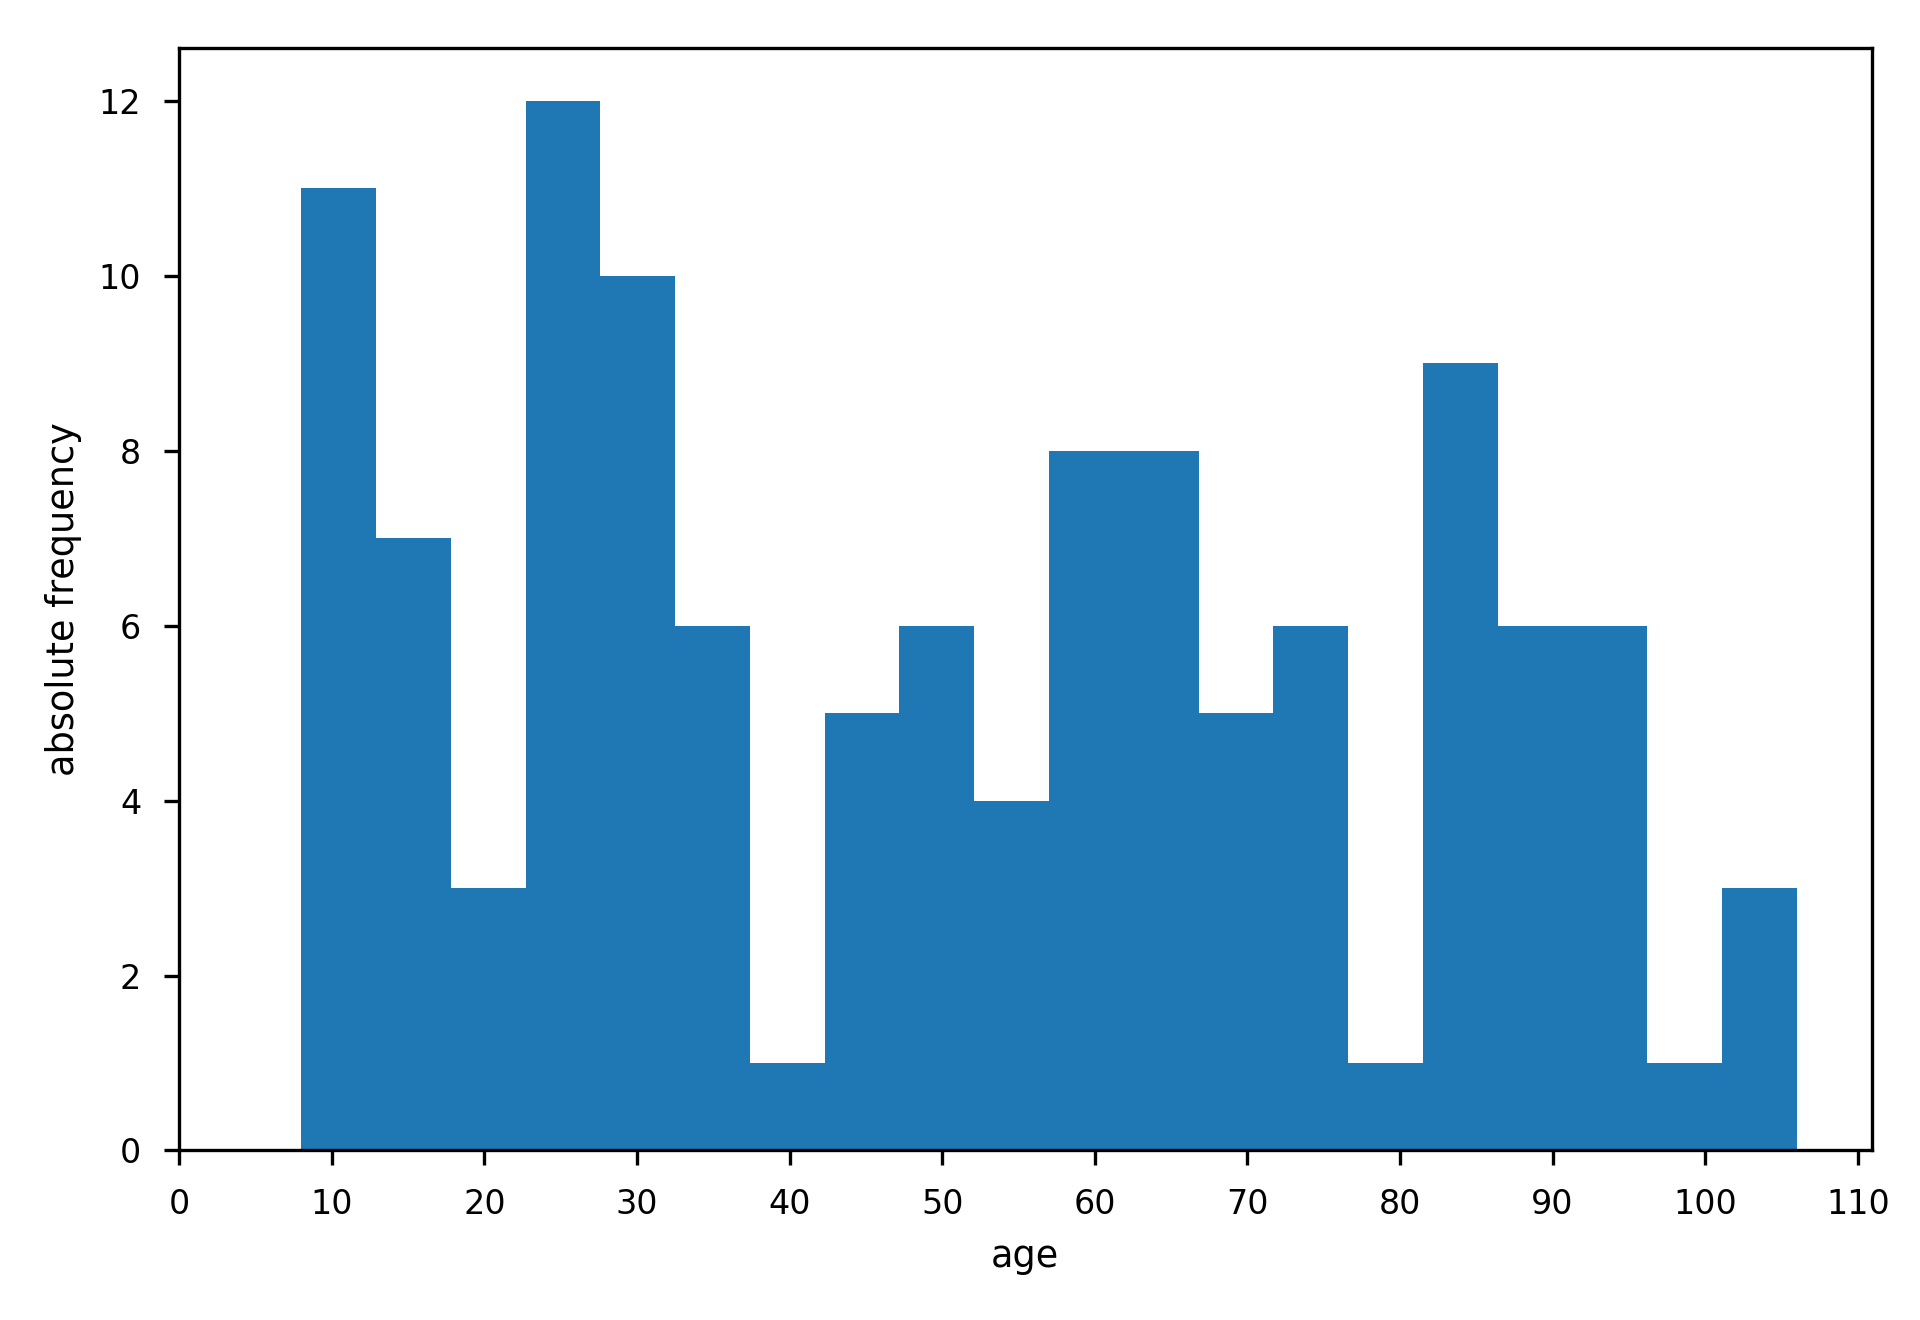
\includegraphics[width=0.8\textwidth]{part2/aging_agehist.png}
	\caption{Age distribution of the $118$ individuals involved in the study.} \label{fig:frassoni_agehist}
\end{figure}

Next, we aim at investigating on how the distribution of the molecular biomarker is influenced by the age of the individuals. To this aim we group the measures per decade and we represent the distribution with boxplots, see Figure~\ref{fig:frassoni_boxplot}.
As we can see, most of the biomarkers show a clear trend with the age. In particular, focusing our attention on the \atpamp ratio ($3^{\text{rd}}$ row, $3^{\text{rd}}$ column of Figure~\ref{fig:frassoni_boxplot}), which is known to be an energy status monitor of the cells, we can see that the values decrease progressively with the decades, with a drastic decrease between $40$ and $50$ years. Moreover, from an observation of \atp and \amp intracellular concentration ($3^{\text{rd}}$ row, $1^\text{st}$ and $2^\text{nd}$ column, respectively) we can sense how the increase of their ratio is mainly due to the grow of \amp in the aging process.


\begin{figure}[]
	\centering
	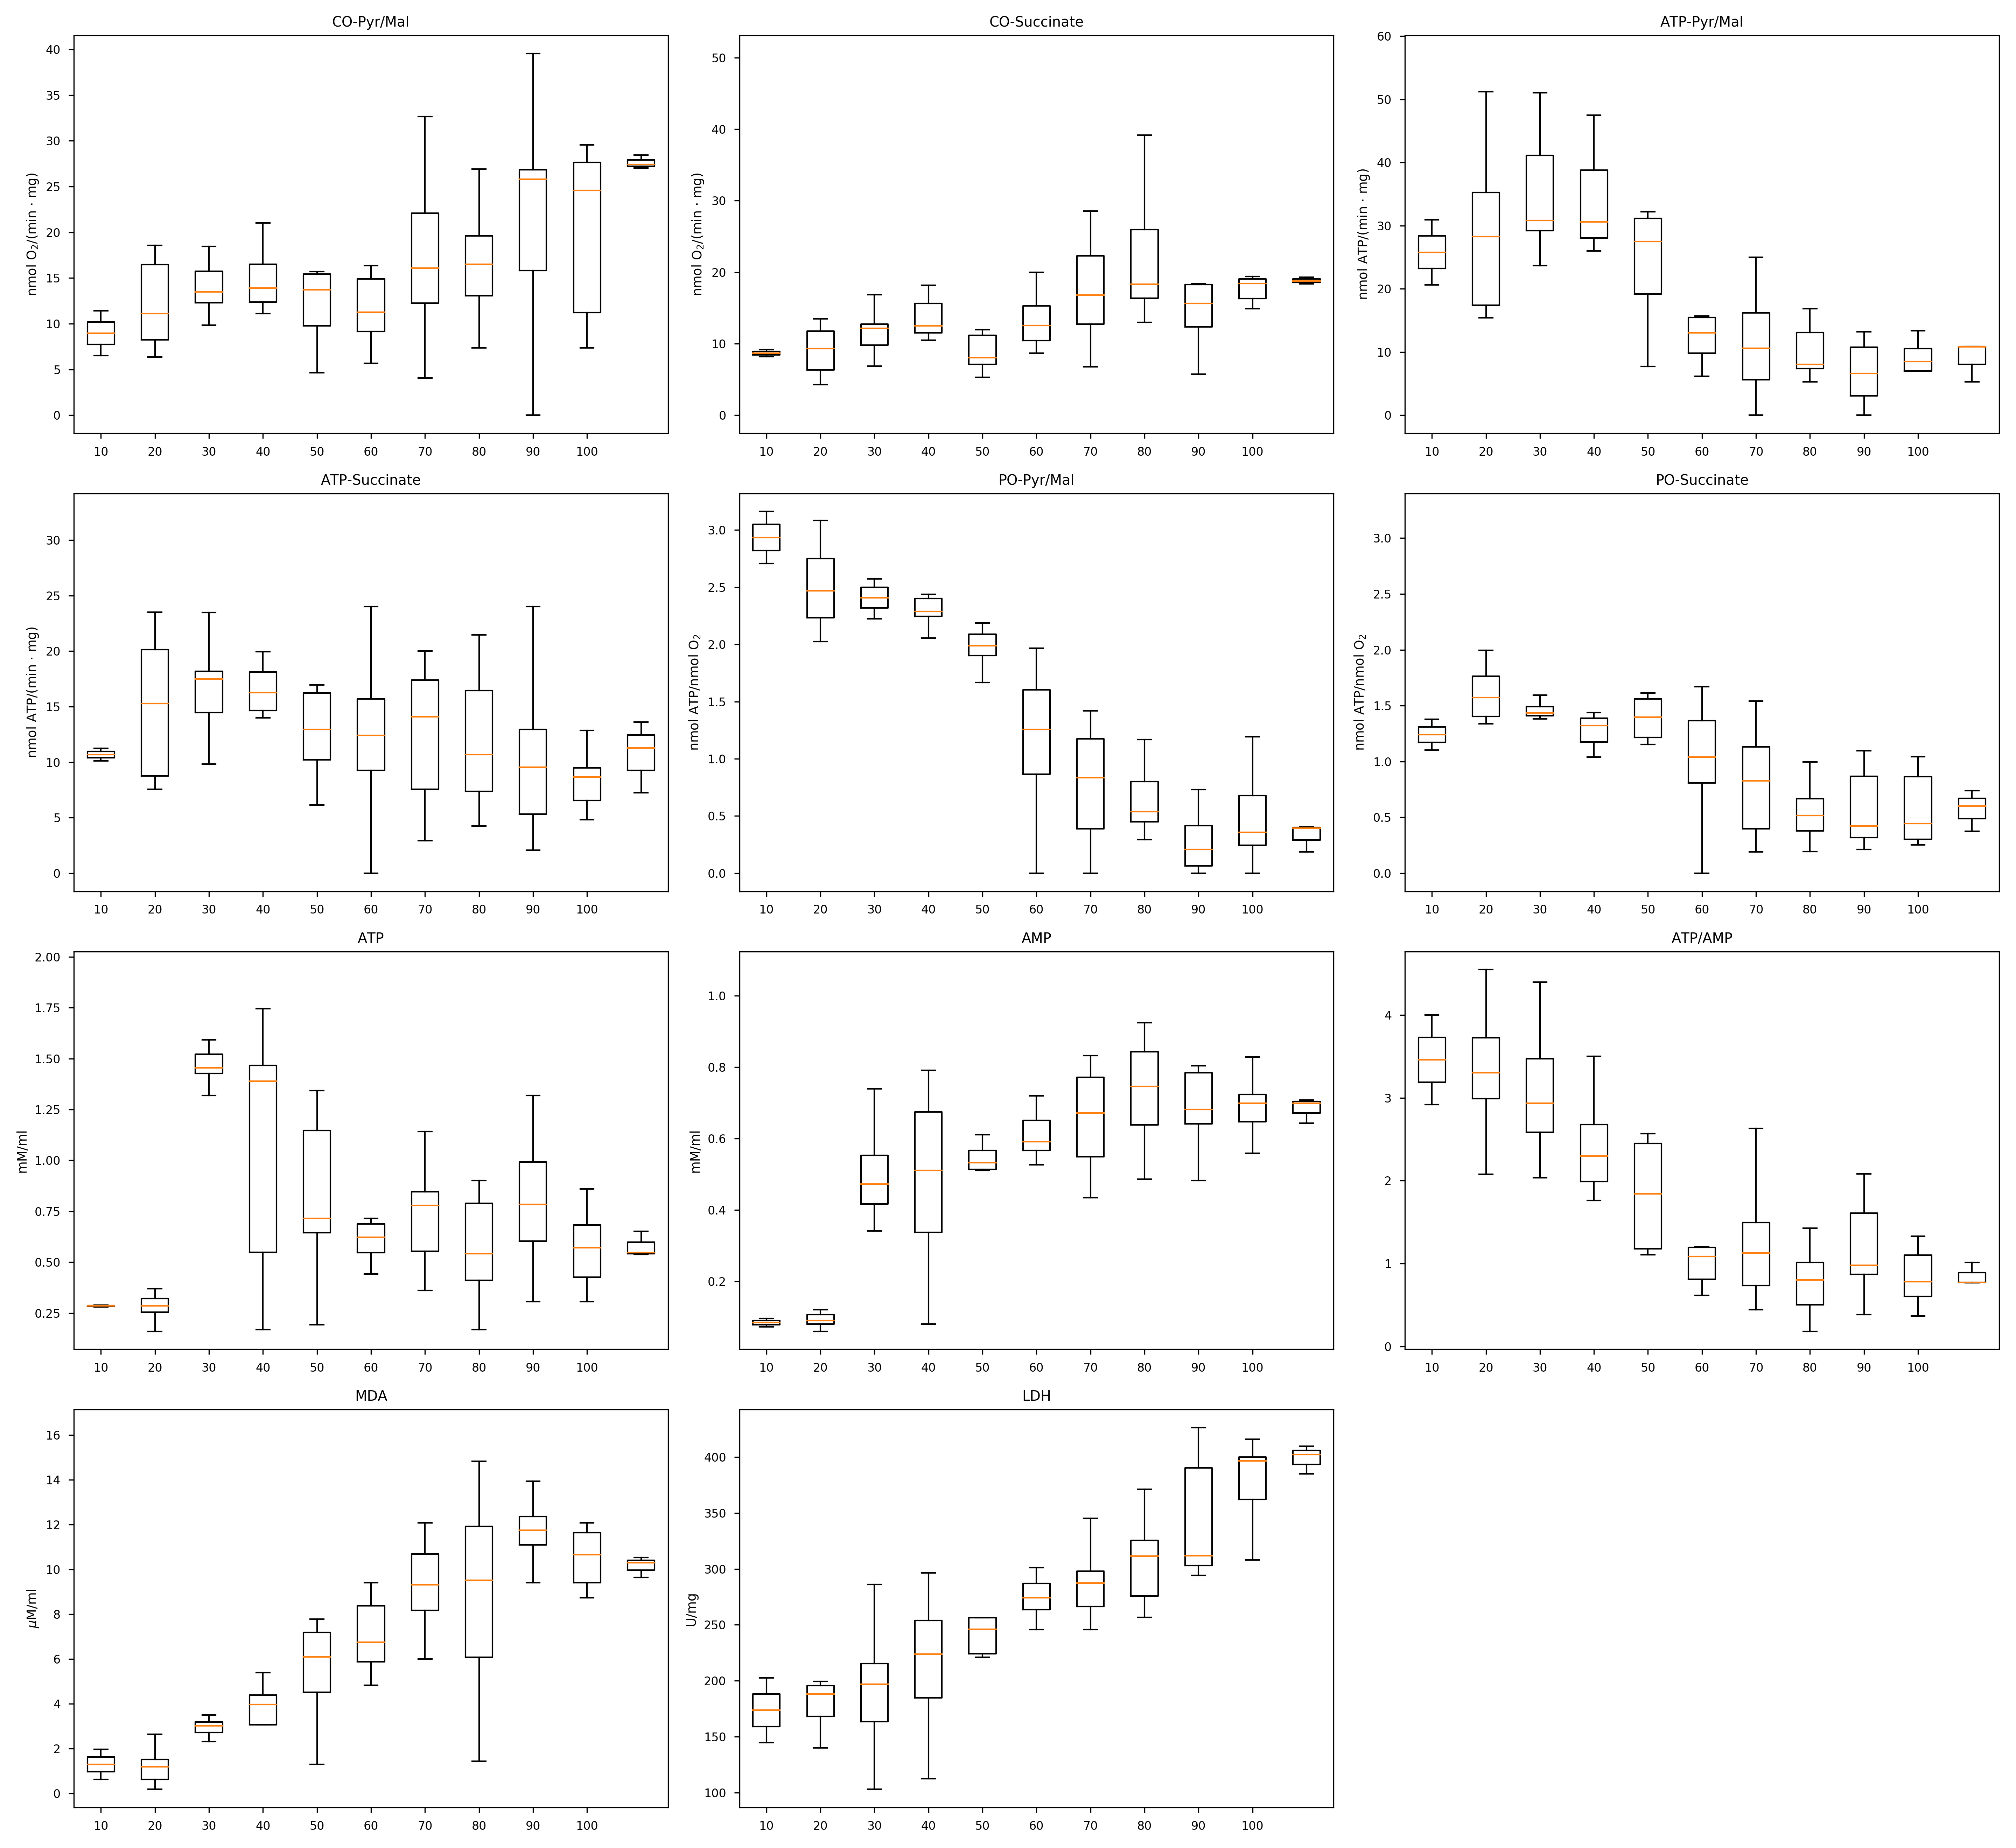
\includegraphics[width=0.8\textwidth]{part2/aging_boxplot.png}
	\caption{Distribution of the collected biomarkers grouped per decade.} \label{fig:frassoni_boxplot}
\end{figure}


\section{Metabolic age prediction} \label{sec:frassoni_regression}
% pipeline + assessment + model challenge

\section{Results} \label{sec:frassoni_results}
% tabella dei risultati

\section{Conclusions and future works} \label{sec:frassoni_conclusions}
% CCS

future: collect more data in order to have a uniformly distributed dataset

%%
% !TEX root = ../main.tex

\chapter{Temporal prediction of multiple sclerosis evolution from patient-centered outcomes} \label{chap:aism}
% AISM

\begin{displayquote}
%	This chapter describes a patient-centered outcomes-based ML model that predicts the disease evolution of multiple sclerosis patients.
	In this chapter, we investigate on
	use of patient-centered outcomes to predict the evolution of multiple sclerosis and to assess its impact on patients' lives.
	Multiple Sclerosis is a degenerative condition of the central nervous system that affects nearly $2.5$ million of individuals in terms of their physical, cognitive, psychological and social capabilities. Despite the high variability of its clinical presentation, \textit{relapsing} and \textit{progressive} multiple sclerosis are considered the two main disease types, with the former possibly evolving into the latter.
	%Nowadays no acknowledged clinical tests to diagnose multiple sclerosis or to distinguish between its types have been proposed.
	Recently, the attention of the medical community toward the use of patient-centered outcomes in multiple sclerosis has significantly increased. Such patient-friendly measures are devoted to the assessment of the impact of the disease on several domains of the patient life.
	% One of the open questions in the field is the use of patient-centered outcomes to assess multiple sclerosis impact on patients' lives and to predict the evolution of the disease.
	%To date, a clear understanding on whether it is possible to define a predictive model based on them is still an open question.
	%the use of such measures to assess neurodegenerative diseases evolution is still lacking. Moreover,
	To this aim, we build a novel temporal model based on gradient boosting classification and multiple-output elastic-net regression. The model
	%  is entirely based on patient-centered outcomes and it
	provides clinically interpretable results along with accurate predictions of the disease course evolution.
\end{displayquote}

\section{Introduction: the evolution of multiple sclerosis} \label{sec:aism_intro}

Multiple Sclerosis (MS) is a neurodegenerative and chronic disease of the central nervous system characterized by damages to the myelin sheaths, resulting in a wide range of symptoms, such as fatigue, numbness, visual disturbances, bladder problems, mobility issues and cognitive deficits.

% \todo{In clinical practice, accurate patient evaluation and clinical judgement remain the basics in MS diagnosis, as the identification of a validated set of biomarkers is still an open problem~\cite{milo2014revised}.}

People with MS (PwMS) are mainly classified according to their disease course:
relapsing-remitting (\ac{RR}), secondary-progressive (\ac{SP}), primary-progressive (\ac{PP}) and progressive-relapsing (\ac{PR})~\cite{giovannoni2016brain} and benign (\ac{B}).
Neurological disability in \RR patients is mainly due to the development of multifocal inflammatory lesions and it results in relapses, that are attacks of neurological worsening (\ie \textit{relapses}), followed by partial or complete recovery. Disability accrues predominantly in progressive courses (\SP, \PP, \PR) that are more characterized from diffuse immune mechanisms and neurodegeneration.
Benign MS occurs when the patient remains fully functional in all neurologic systems for at least $15$ years after the onset.
Figure~\ref{fig:ms_mock} shows a representative disability progression of MS patients according to their disease course.

An estimated $15\%$ of PwMS have a \PP or \PR course at the onset, the remaining $85\%$ is diagnosed with a \RR course.
About $80\%$ of \RR patients develop \SP course within $15\text{--}20$ years if untreated, or if the adopted pharmacological and rehabilitative protocols are not continuously adjusted according to the evolution of the disease~\cite{scalfari2014onset}.

\begin{figure}[]
	\centering
	\subfloat[]{%
		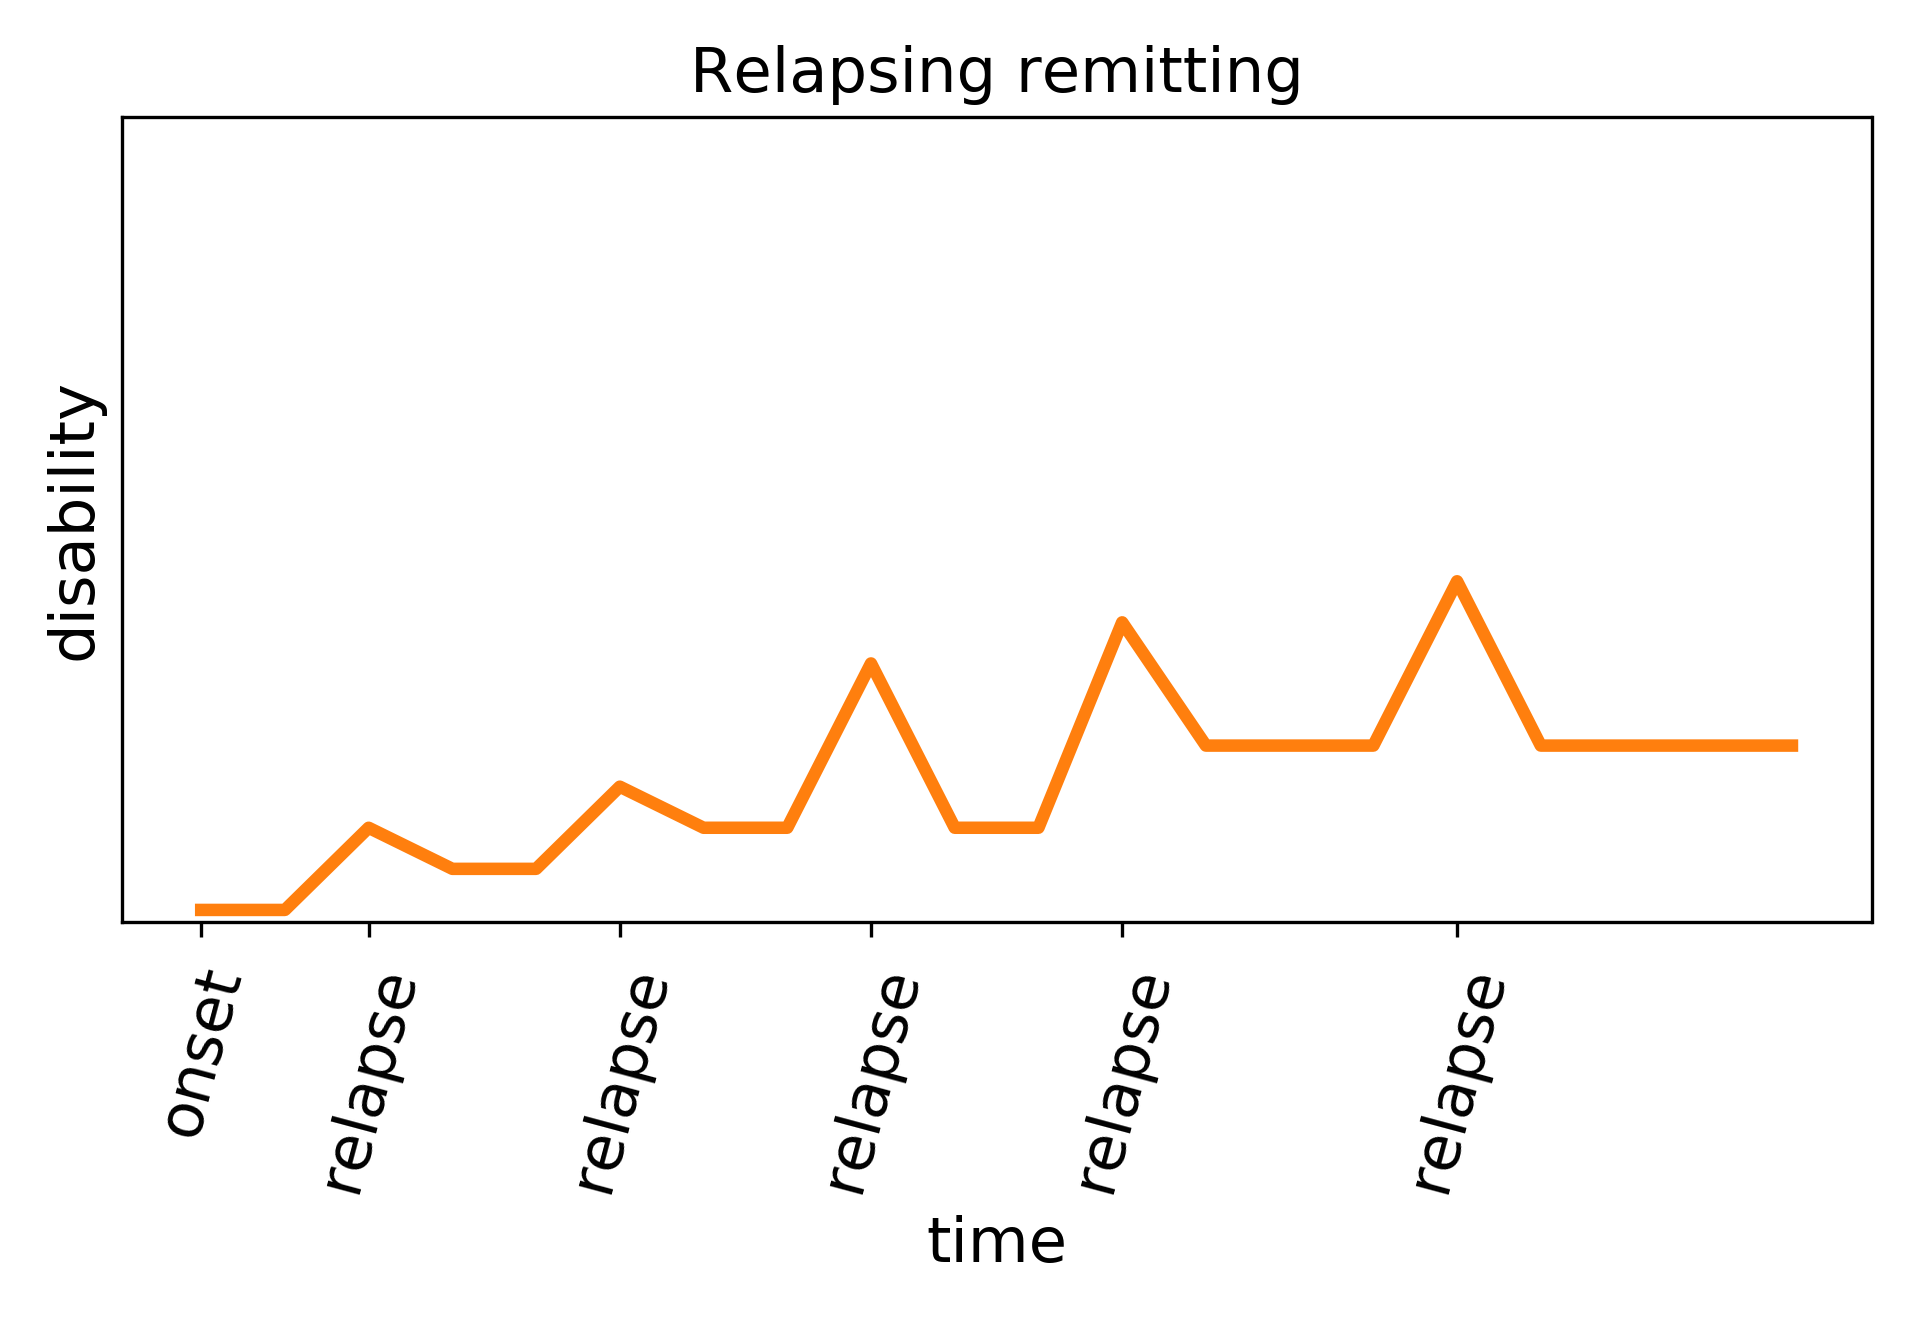
\includegraphics[width=0.5\textwidth]{part2/ms_mock_rr.png}
		\label{fig:ms_mock_rr}%
	}%
	\subfloat[]{%
		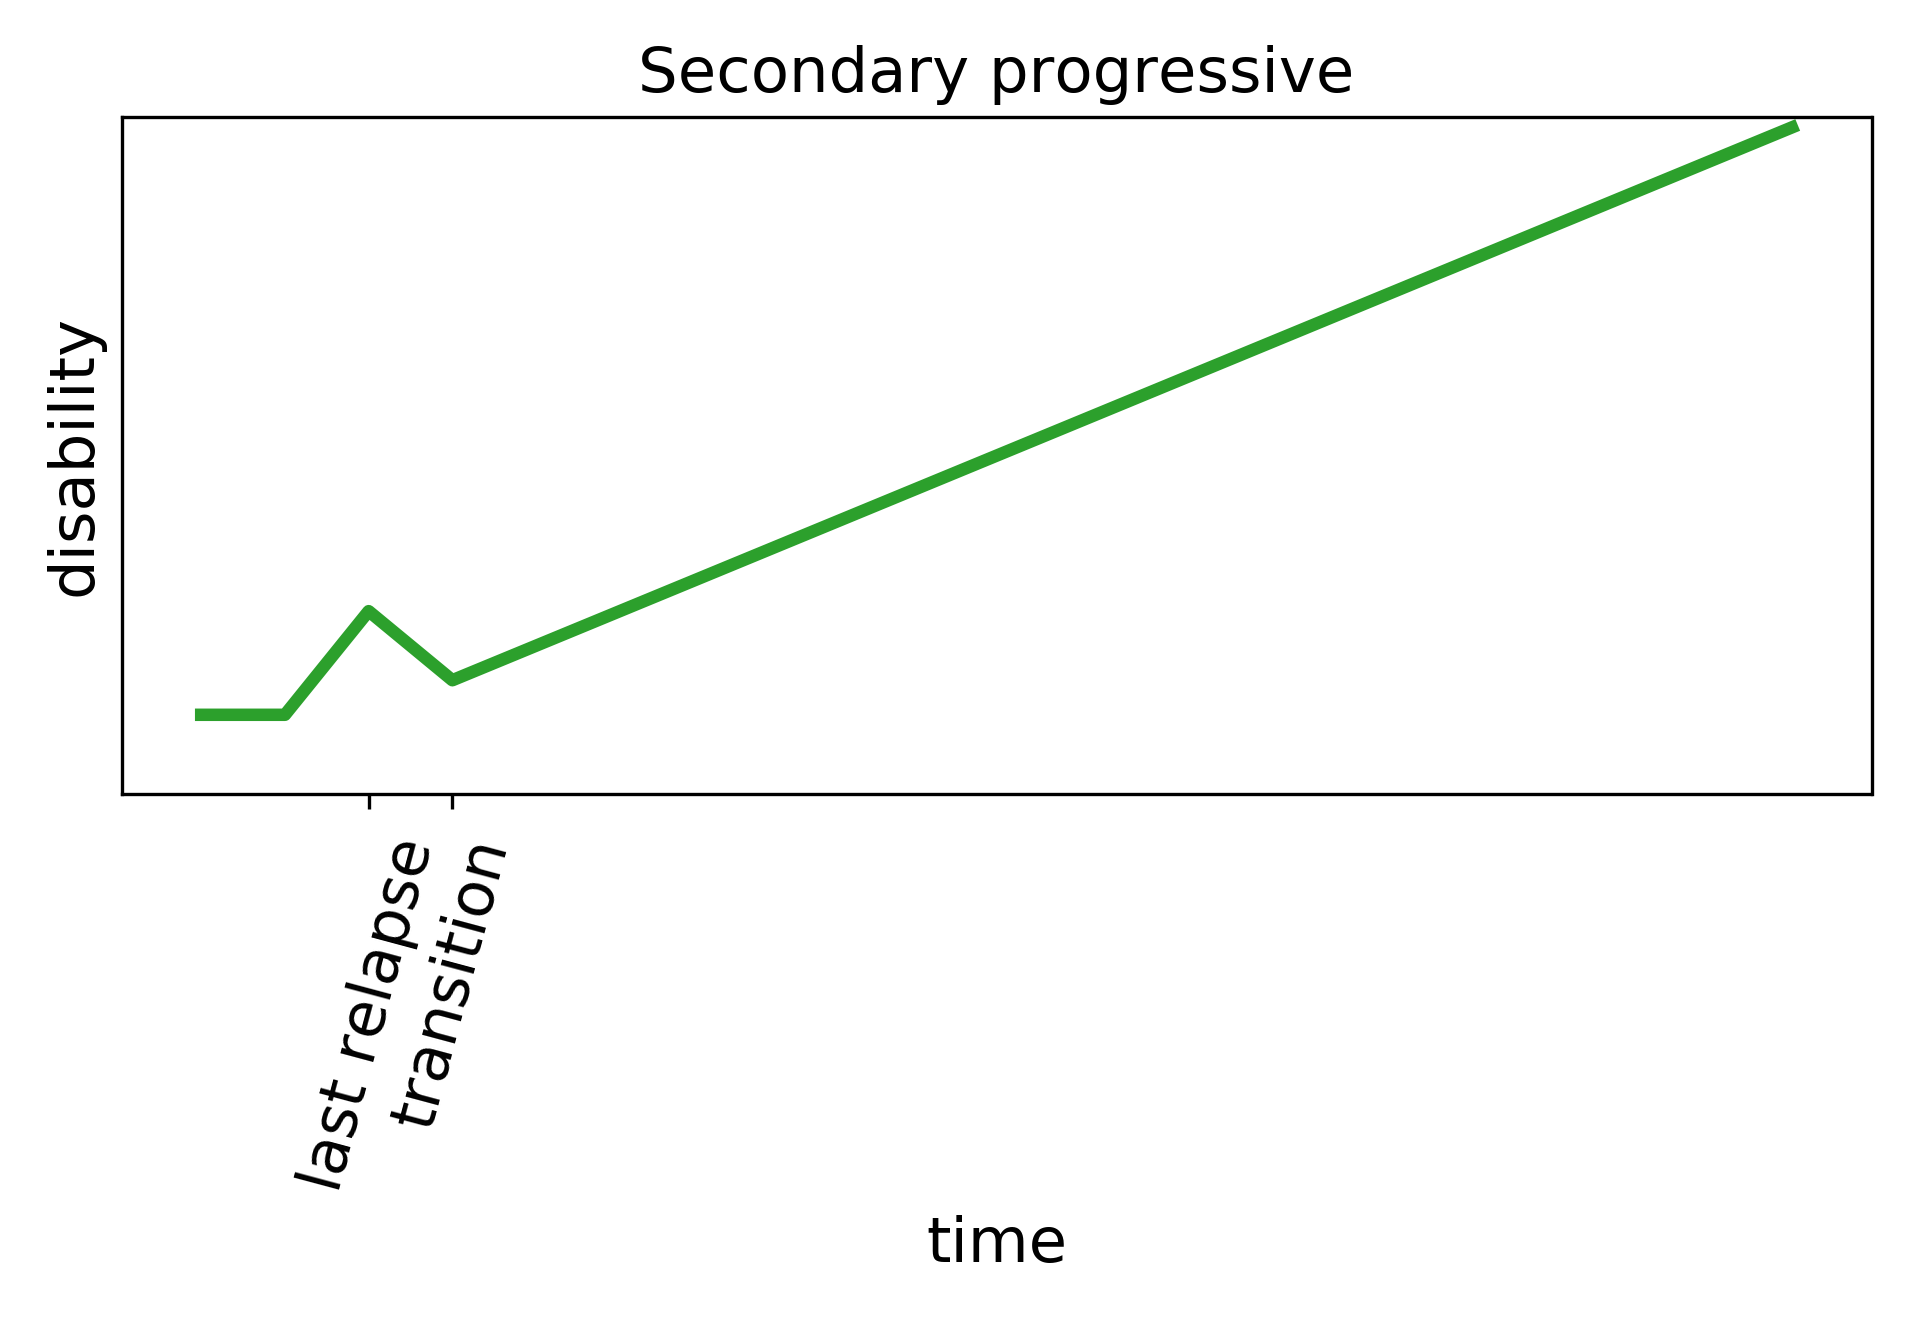
\includegraphics[width=0.5\textwidth]{part2/ms_mock_sp.png}
		\label{fig:ms_mock_sp}%
	}
	\hfill
	\subfloat[]{%
		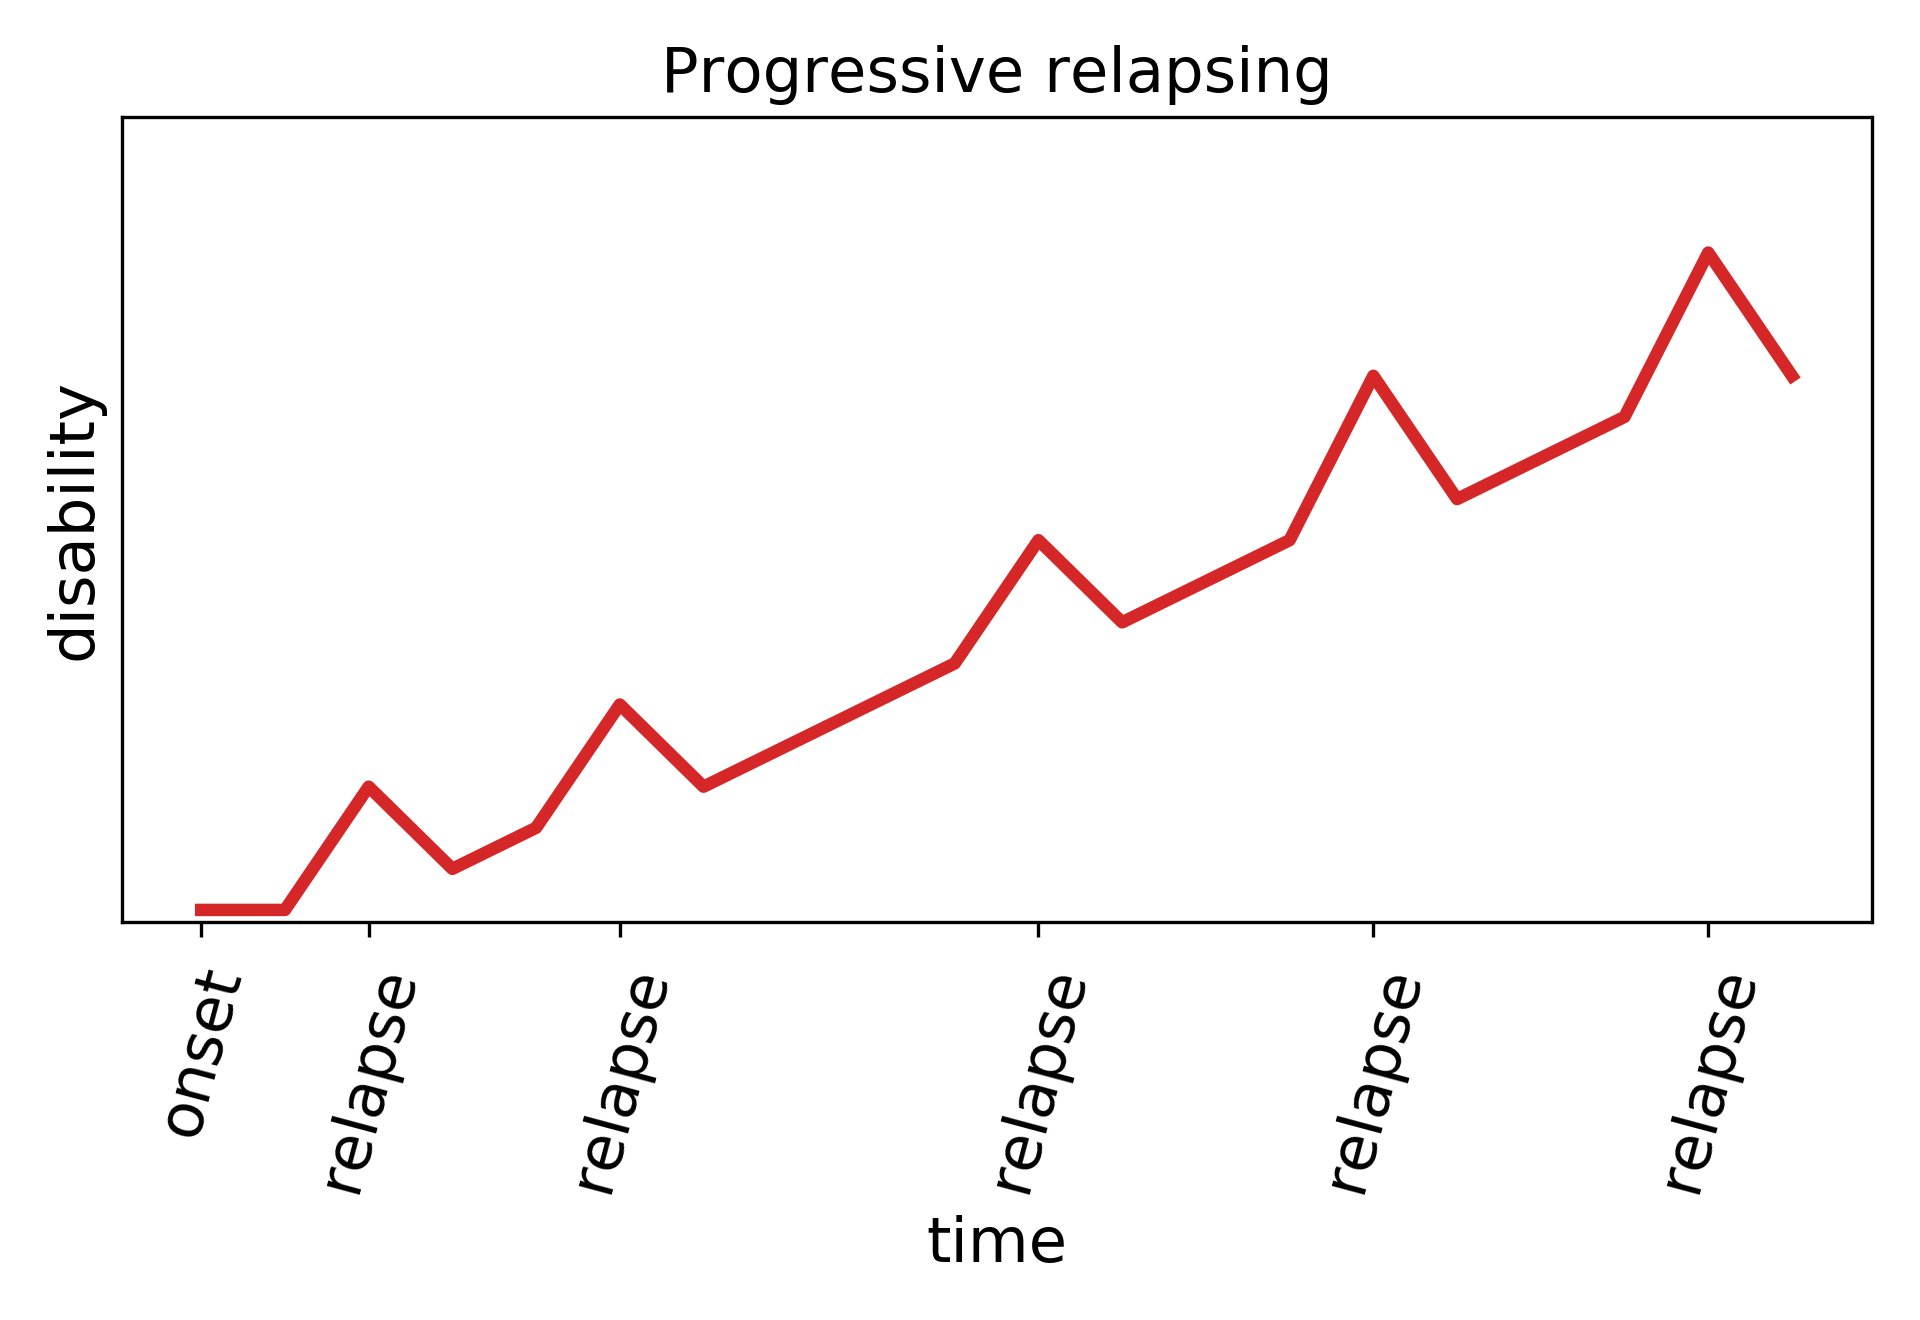
\includegraphics[width=0.5\textwidth]{part2/ms_mock_pr.png}
		\label{fig:ms_mock_pr}%
	}%
	\subfloat[]{%
		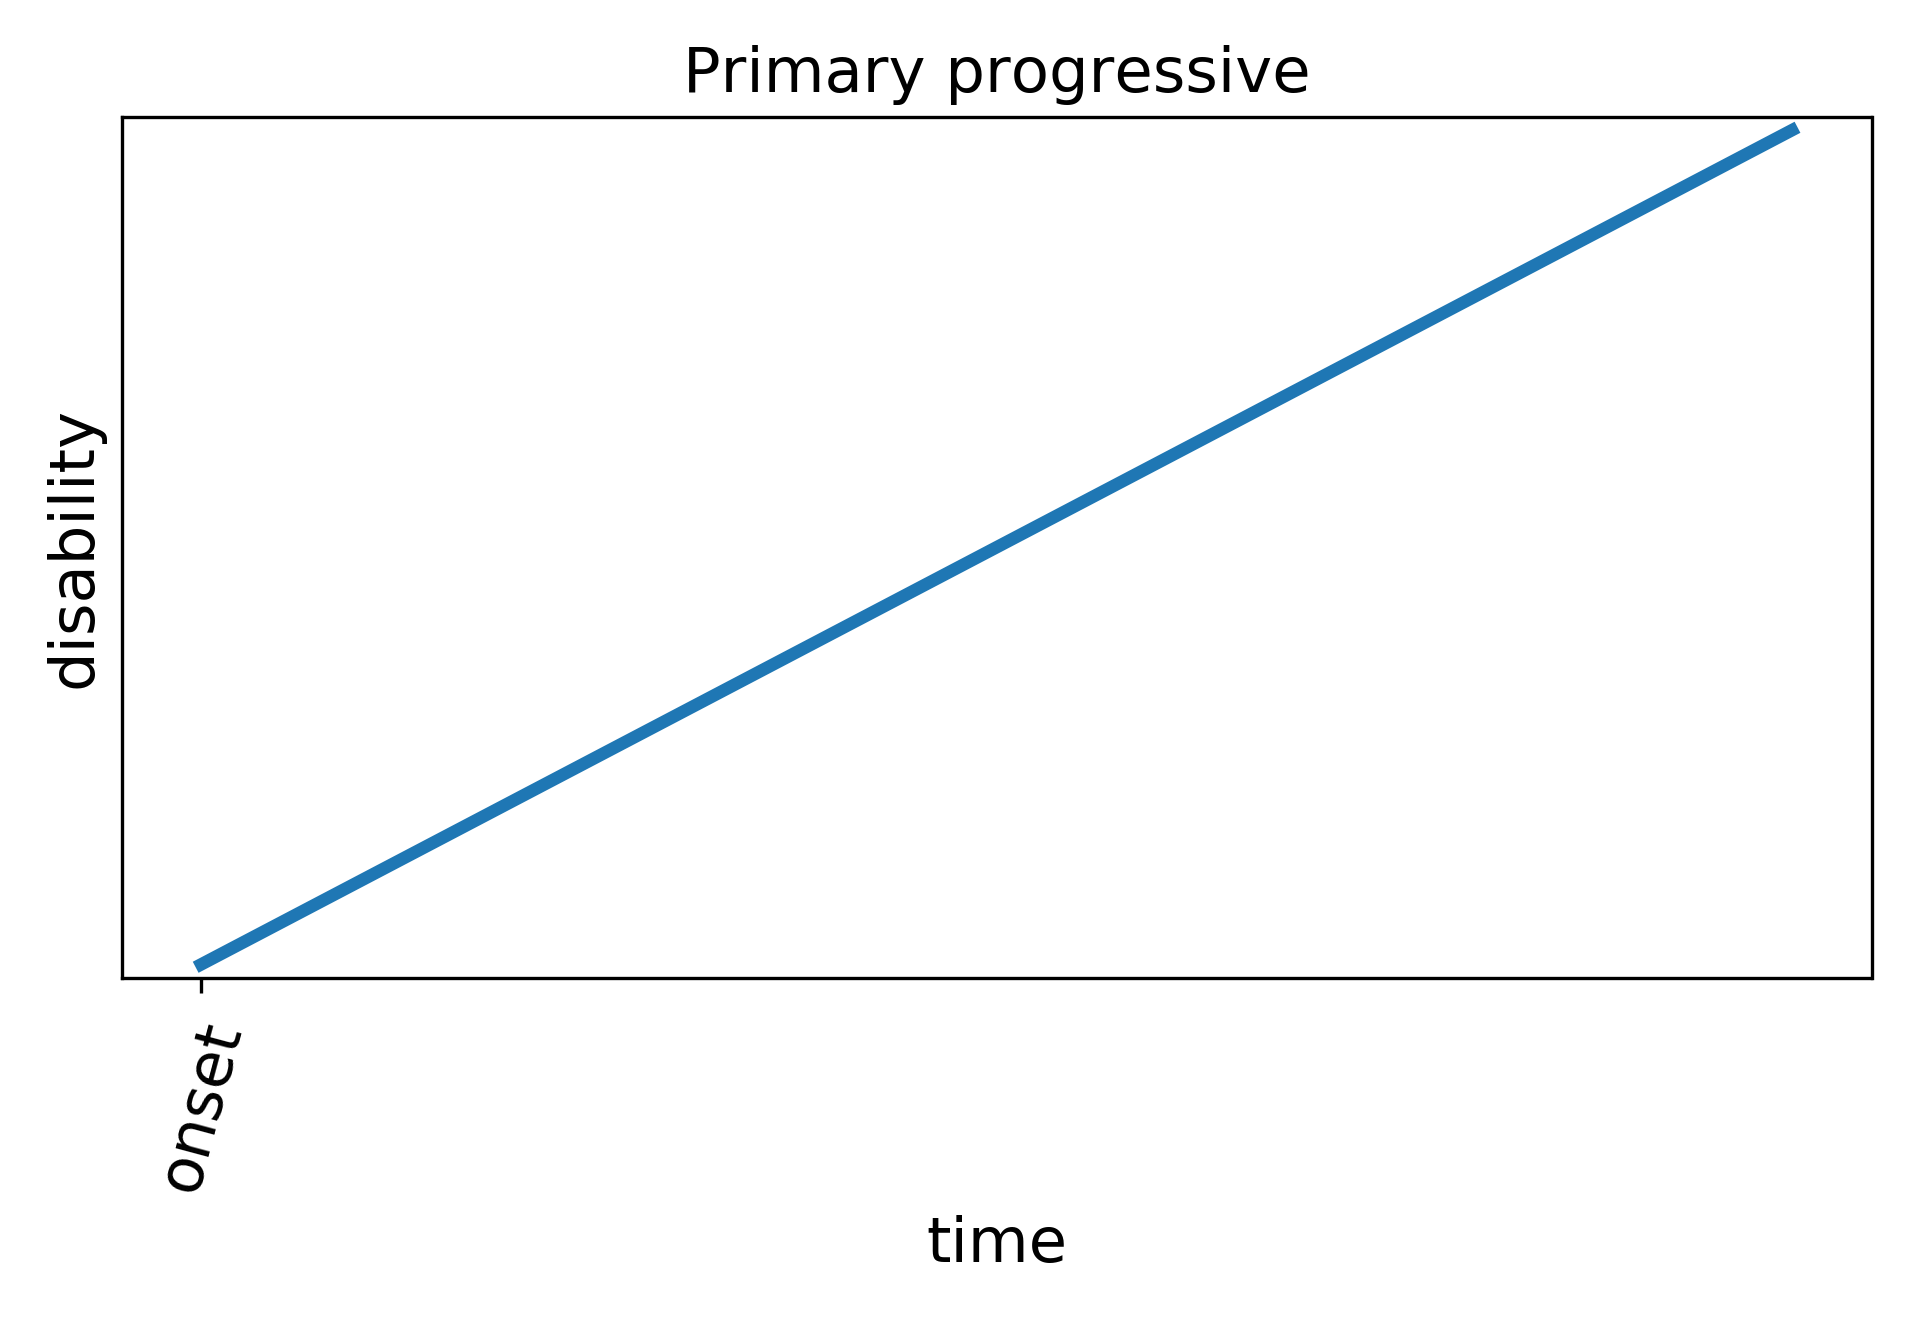
\includegraphics[width=0.5\textwidth]{part2/ms_mock_pp.png}
		\label{fig:ms_mock_pp}%
	}
	\caption{Disability evolution of the four main MS courses: panel (a) shows a prototypical \RR patient, characterized by time-limited attacks which may or may not leave permanent deficits; panel (b) shows \SP typical disability progression, that is steady with no more relapses; panel (c) represents a typical \PR disability evolution, which is characterized by steady disability progression from the onset; panel (d) shows a \PR patient; which has a steady disability progression from the onset with relapses.} \label{fig:ms_mock}
\end{figure}


% This form is characterized by clearly defined {\em relapses}, \ie  attacks of neurological worsening, followed by partial or complete recovery.
% and it takes only $14$ years on average for people to become unable to walk for $100$ meters unaided .
% Patients in \SP form experience a steady progress of the disease in absence of relapses, while patients in \PR form are characterized by both relapses and gradual worsening.

For this reason, the prediction of the transition from \RR to \SP is one of the most important methodological gaps that MS researchers are currently addressing.
The availability of a statistical model able to predict disease worsening is one of the major unmet needs that could significantly improve timeliness, personalization and, consequently, the efficacy of the treatments.
Nowadays, there are no clear clinical, imaging, immunologic or pathologic criteria to foresee the transition from \RR~to~\SP~\cite{lublin2014defining}. Several clinical factors relating to possible \SP course predictors have been identified~\cite{bergamaschi2015bremso, dickens2014type}.
However, as showed by~\cite{vukusic2003prognostic}, studies investigating on prognostic factors for MS course evolution generally suffer from two shortcomings: they
% However, such studies generally
report a high proportion of \RR patients not monitored enough to reach progressive course and they lead, to some extent, to contradictory results.
Currently, MS research mainly focuses on developing and assessing drugs and rehabilitative protocols for \RR patients disregarding progressive courses.

\section{\PCOs data collection}\label{sec:proms_data_collection}

In the recent past, researchers explored the potential role of Patient-Centered Outcomes (\ac{PCO}) to follow the progression of neurodegenerative diseases and to take timely decisions~\cite{black2013patient}. %~\todo{REF \cite{??}}.
%\PCOs usually consist in ordinal or categorical scaled questionnaires and self-reported measures.
\PCOs comprise self- and physician-administered tests, questionnaires and clinical scales consisting of either ordinal or categorical scaled answers.
As opposed to stressful, not frequently repeatable and expensive clinical exams, like magnetic resonance imaging or blood tests, \PCOs are patient-friendly and low-cost measures that could allow to investigate the individual changes and disease impact on several aspects such as physical, cognitive, psychological, social and well-being domains~\cite{fiorini2015machine}.
%.
To date, \PCOs are extensively used to assess general health status, to support diagnosis and monitor progress of disease and to quantify the patients' perception of the effectiveness of a given therapy or procedure \cite{nelson2015patient}.
Nevertheless, it is still unclear which are the most informative \PCOs and, contextually, whether they can be used as {\em predictors} for disease evolution.

%\todo{In our study, we propose a machine learning approach that, leveraging on \PCOs data, aims at
%forecasting the transition of PwMS from \RR to \SP and at providing insights on the most appropriate use of \PCOs.}
%In our study, we propose a machine learning approach that, leveraging on \PCO data, aims at predicting the temporal evolution of MS disease course providing insights on the most appropriate use of \PCOs.
%We resort to a vast category of predictive models, ranging from sparse regularization to ensemble and deep learning methods.
%These models are widely adopted in the biomedical context as they benefit from good generalization properties as well as they allow to address regression and classification problems within the same statistical and computational framework~\cite{lecun2015deep, qi2012random, nowak2011fused,  teramoto2009balanced, zou2005regularization}.
%azencott2013efficient

% \PCOs are low-cost and patient-friendly source of information that can be acquired over time in order to quantitatively assess patients' disease impact on several aspects of their life.

The biomedical data science challenge presented in this chapter is based on a \PCO dataset acquired from a cohort of PwMS progressively enrolled within an ongoing funded project \footnote{ethical review committee approval \textit{023REG2014} was obtained for this work}.

Each patient is evaluated every four months through the items of the \PCOs reported in Table~\ref{tab:proms} which cover physical, cognitive and psychosocial domains. A comprehensive description of the \PCOs involved in the study is presented below.


\begin{itemize}
	\item[] {\sc \textbf{MFIS}} This is a $21$-item self-reported questionnaire typically administered in $5$ to $10$ minutes. \MFIS provides an assessment of the effects of fatigue in terms of physical, cognitive, psychosocial functioning and it is considered a valuable tool by clinicians.
	
	\item[] {\sc \textbf{HADS}} This is a $14$-item self-reported questionnaire typically administered in $2$ to $6$ minutes which aims at detecting clinically significant symptoms of depression and anxiety in patients. \HADS consists in $7$ questions for depression and the remaining $7$ for anxiety.
	
	\item[] {\sc \textbf{LIFE}} This is an $11$-item self-reported questionnaire which investigates on patients quality of life. \LIFE can be typically administered in approximately $5$ minutes. To each of the $11$ items, the patient can assign an ordinal score $0,1,2$ which corresponds to "\textit{disagree}", "\textit{not sure}" and "\textit{agree}" answers.
	
	\item[] {\sc \textbf{OAB}} This is an $8$-item self-reported questionnaire which investigates on patients bladder control. \OAB can be administered in approximately $5$ to $8$ minutes and it is a reliable tool to investigate on possible stress or discomfort lead by unexpected urinary urgencies that patients may experience during day or night.
	
	\item[] {\sc \textbf{EDINB}} This $10$-item self-reported questionnaire can be used to assess dominance of a person's right/left hand during daily activities. The items are very straightforward, so \EDINB can be administered in $3$ to $5$ minutes.
	
	\item[] {\sc \textbf{ABILH}} This is a $23$-item self-reported questionnaire which can be used to measure hand ability in adults with upper limb impairments. \ABILH assesses a person's ability to manage daily activities that require the use of the upper limbs, whatever the strategies involved. \ABILH is usually administered in $5$ to $10$ minutes.
	
	\item[] {\sc \textbf{FIM}} This is $19$-item clinical scale assessing the amount of assistance required for the patient to carry out activities of daily living. \FIM is typically administered by trained examiner in $35$ to $40$ minutes and it covers both motor and cognitive domains.

	\item[] {\sc \textbf{MOCA}} This is an $11$-item clinical scale assessing several cognitive domains such as short-term memory recall, visuospatial abilities, phonemic fluency, attention, concentration and so on. \MOCA is typically administered in less than $10$ minutes.
	
	\item[] {\sc \textbf{PASAT}} This clinical scale is a measure of cognitive function that assesses patients' auditory processing speed and flexibility,  as well as their calculation ability. It can be administered in $10$ to $15$ minutes and it consists in audio stimuli in which single digits are presented every $3$ seconds. The patient is asked to add each new digit to the one immediately prior to it. \PASAT must be administered by trained examiner.
	
	\item[] {\sc \textbf{SDMT}} This clinical scale is a test for organic cerebral dysfunctions. This test simply involves a substitution task: using a reference key the patients has few seconds to pair specific numbers with specific geometric measures.
	\SDMT is typically administered by trained examiner in less than $5$ minutes.
	
	\item[] {\sc \textbf{EDSS}} This is probably the oldest assessment instrument for MS. \EDSS is based on a neurological examination consisting of $7$-items. Each item rates a different function, all the items are then combined in the final \EDSS score which is an ordinal scale ranging from $0$ (normal neurological examination) to $10$ (death due to MS), in half-point increment. The use of \EDSS in modern MS assessment is somewhat controversial. Although usually adopted as an index of the disability level, \EDSS focuses mainly on deambulation disability without taking into account other aspects that could impact patient disability, such as upper limb or cognitive functions~\cite{meyer2014systematic, uitdehaag2014clinical}.
	
	
\end{itemize}

\PCO data are intrinsically noisy due to the subjectivity of self-reported measures provided by the patients that can be influenced by personal feelings and opinions. In order to ameliorate this issue, $4$ questionnaires out of $10$ are administered by medical staff which is trained to keep a homogeneous level of evaluation.

In our analysis we considered all the \PCOs reported in Table~\ref{tab:proms} except \EDSS.
%\todo{other comments here?}

% The model considered all the \PCOs except \EDSS, that is a physician reported outcome that, although usually adopted as an index of the disability level, exclusively depends on the deambulation for scores greater than 4, consequently not taking into account the other aspects impairing the patient.

\begin{table}[htb]
	\center
	\footnotesize
	\begin{tabular}{l|l|l}%{@{} l*{4}{l} @{}}
		\toprule
		Acronym & Full name & Reference \\
		\midrule
		\MFIS & Modified fatigue impact scale & \cite{flachenecker2002fatigue}\\
		\HADS & Hospital anxiety and depression scale &  \cite{honarmand2009validation}\\
		\LIFE &  Life satisfaction index &  \cite{franchignoni1999life}\\
		\OAB & Overactive bladder questionnaire & \cite{cardozo2014validation}\\
		\EDINB &  Edinburgh handedness inventory & \cite{oldfield1971assessment} \\
		\ABILH &  Hand ability index & \cite{arnould2012can} \\
		\midrule
		\FIM &  Functional independence measure  &\cite{granger1990functional}\\
		\MOCA &  Montreal cognitive assessment & \cite{dagenais2013value}\\
		\PASAT &  Paced auditory serial addition task & \cite{aupperle2002three} \\
		\SDMT &  Symbol digit modality test  & \cite{parmenter2007screening}\\
		\EDSS & Expanded disability status scale & \cite{kurtzke1983rating}\\		\bottomrule
	\end{tabular}
	\caption{The set of available \PCOs.
		The first $6$ are self-reported, while the last $5$ are administered by trained medical staff.
		In our analysis all \PCOs were used, with the exception of \EDSS.
		% The set of clinically validated questionnaires available for this work. All questionnaires were used to predict the disease course evolution with exception of \EDSS. The answers to the first $6$ questionnaires are completely self-reported, while the last $5$ are administered by trained medical staff.
	}\label{tab:proms}
\end{table}


% we focus on the use of $10$ of the clinically validated questionnaires reported in Table~\ref{tab:proms}. Each questionnaire consists of a different number of items testing the capabilities of the patients in different domains, such as physical, cognitive or psychosocial.
% Moreover, the set of variables considered by our
The collected \PCO dataset comprises additional information such as:
\begin{enumerate*}[label=\roman*)]
	\item number of relapses in the last four months (NR),
	\item educational level expressed in terms of total years of education (EDU),
	\item height (H) expressed in $\text{cm}$ and
	\item weight (W) expressed in $\text{kg}$.
\end{enumerate*}
Moreover, a neurologist assigns to each patient the corresponding disease course. The global distribution of MS types across time points is depicted in Figure~\ref{fig:PPRRSP}.

% \todo{@AISM: add here the motivations that lead us to exclude \EDSS from the analysis.}

%%%%%%%% EDA %%%%%%%%
\section{\PCOs exploratory data analysis} \label{sec:aism_eda}


 \begin{figure}[]
	\centering
	\subfloat[]{%
		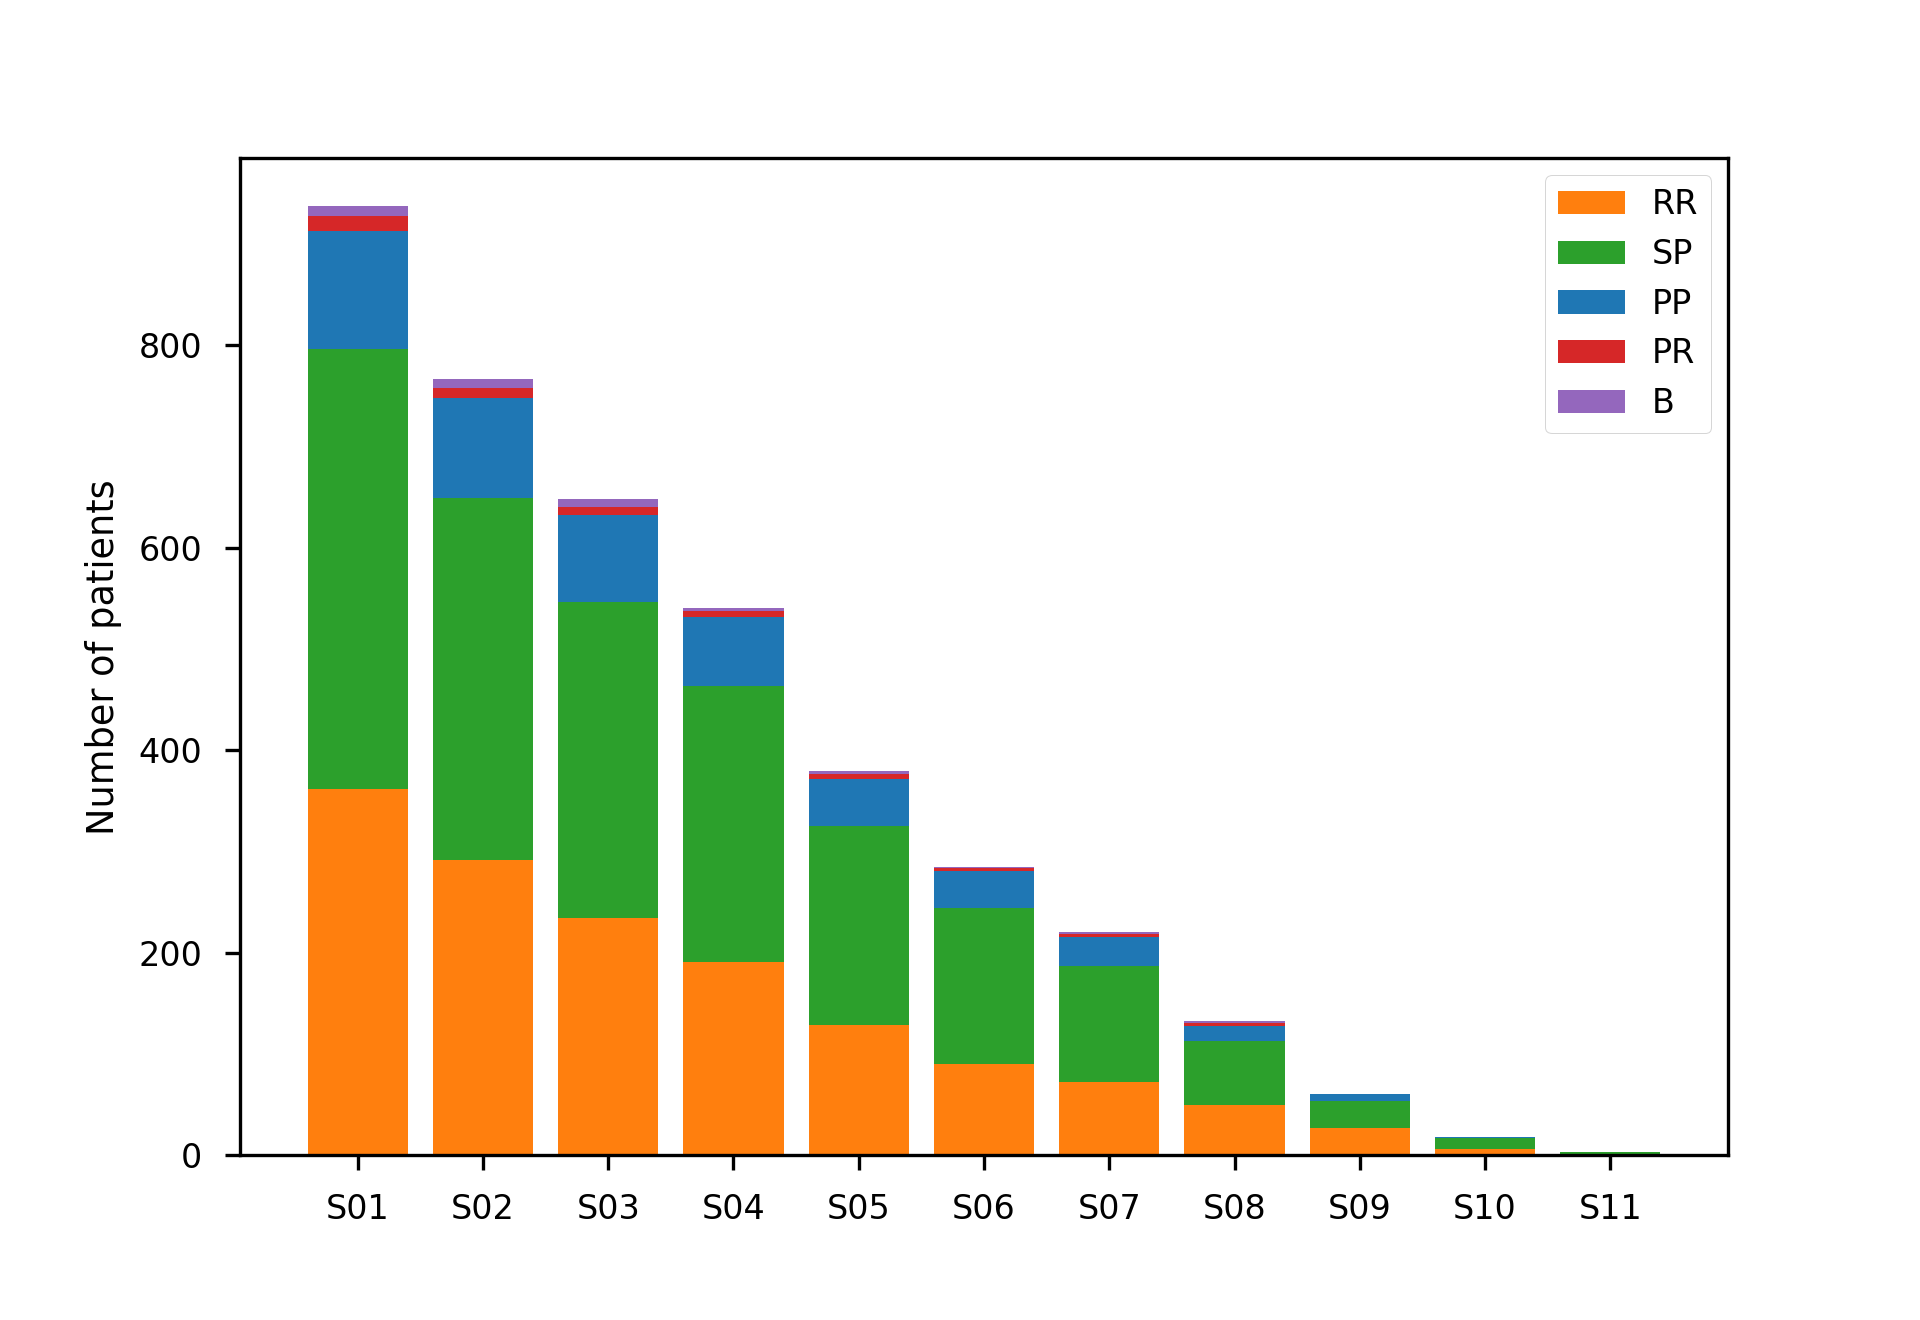
\includegraphics[width=0.5\textwidth]{part2/ms_bars.png}
		\label{fig:patients}%
	}%
	%	\hfill%
	\subfloat[]{%
		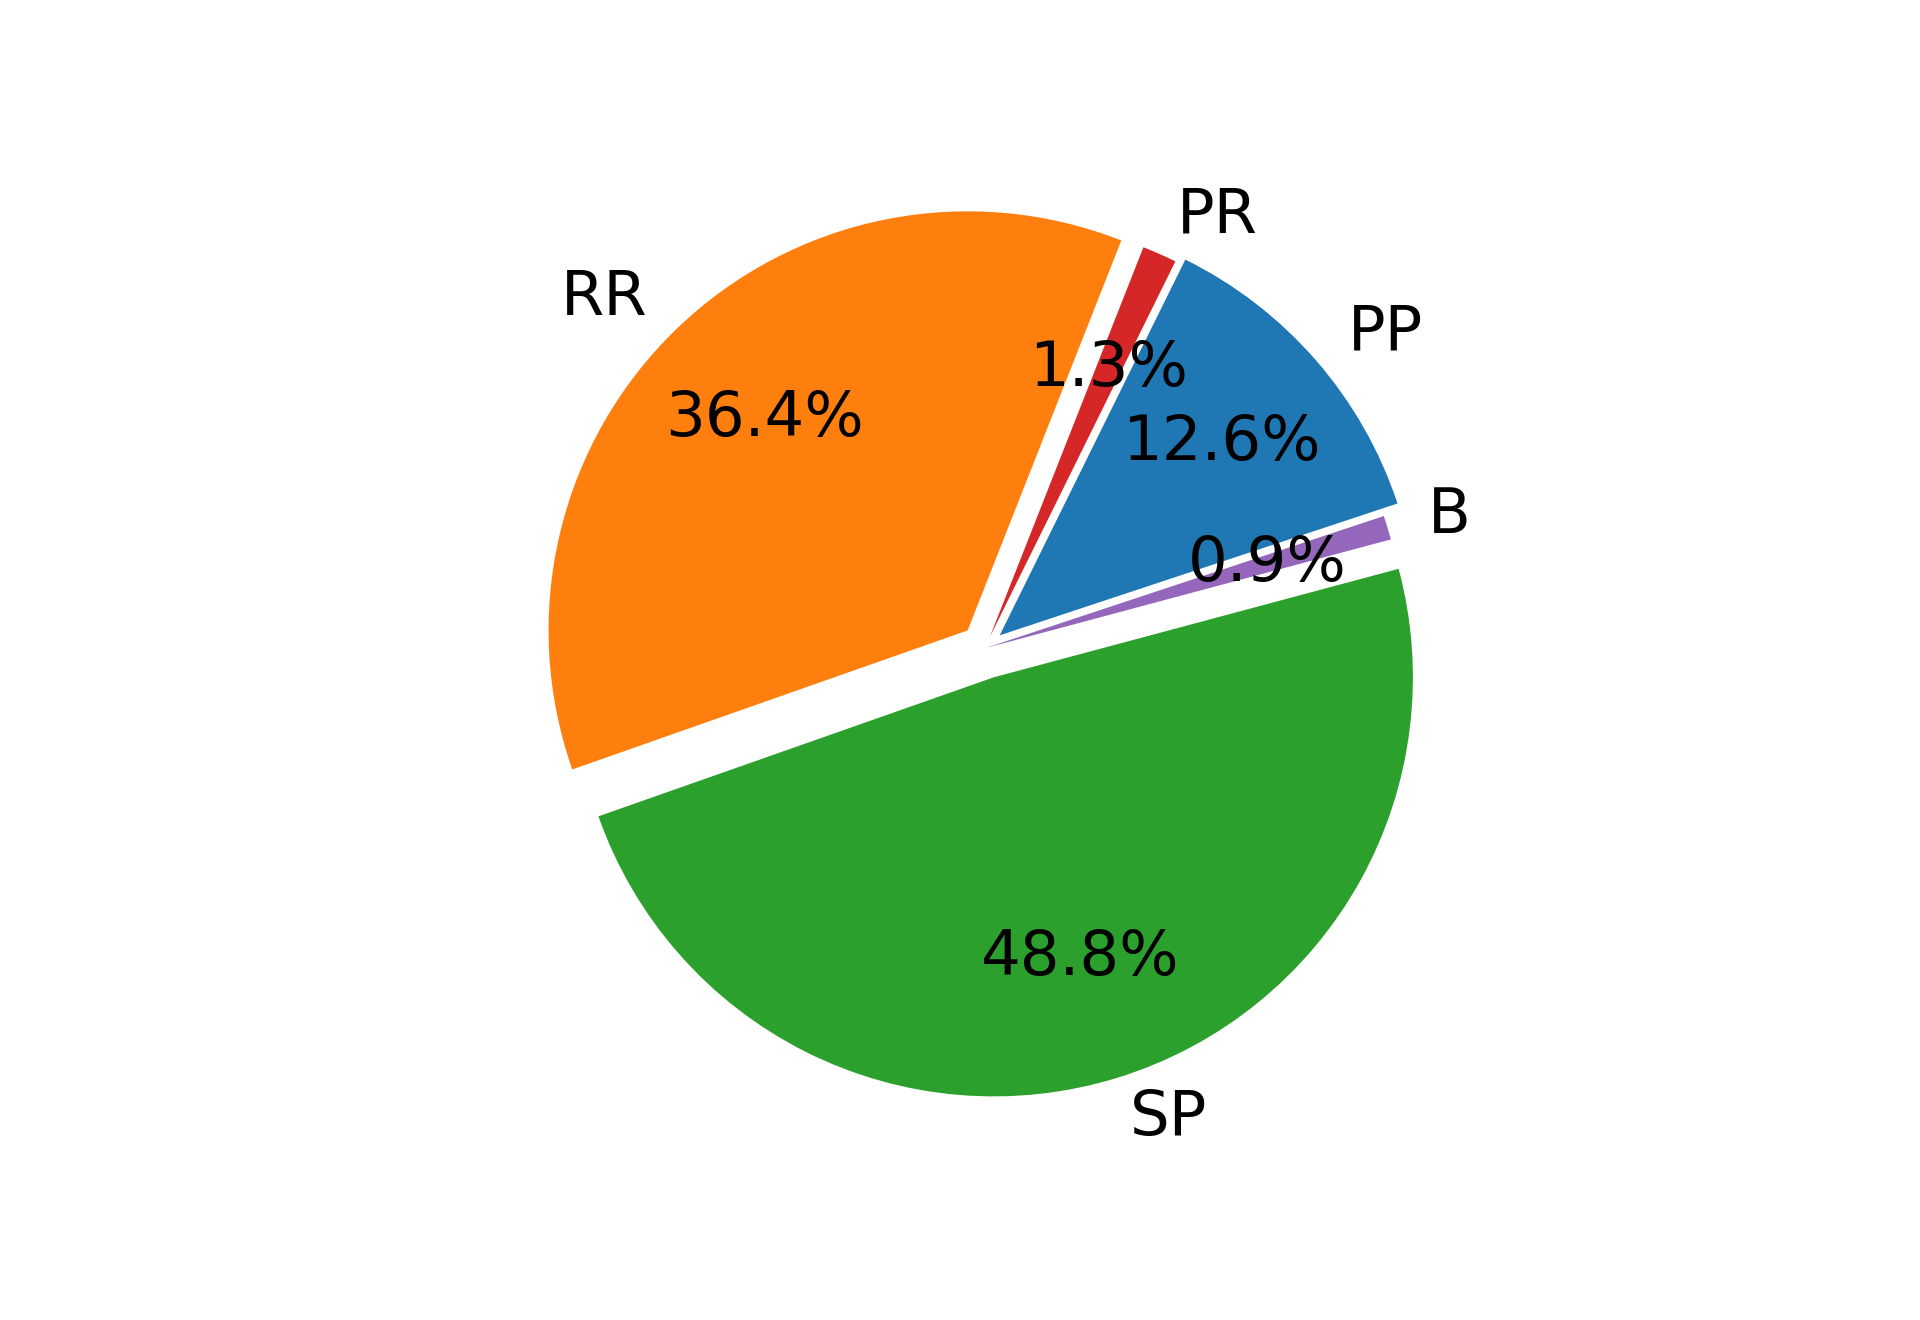
\includegraphics[width=0.5\textwidth]{part2/ms_pie.png} \label{fig:PPRRSP}
	}%
	\caption{An overview of the \PCO dataset used in this study. The left panel (a) shows a bar chart of the number of MS patients in each disease form  at different examinations. The right panel (b) presents a representation of the distribution of the total amount of acquisitions ($3991$), divided according to the disease form.}\label{fig:data}
\end{figure}


%In this work we focus on detecting the \RR to \SP prediction, hence the patients in \PR and \PP form will not be taken into account.

In this work we analyze \PCOs data acquired every four months from a cohort of MS patients enrolled in a funded study.
Currently, we have collected data for $11$ examinations and, as patients enrollment is still ongoing,  the number of individuals for each time point is successively decreasing
Our dataset comprises a grand total of $3991$ patients, with $1451$ \RR, $1947$ \SP, $503$ \PP, $53$ \PR and $37$ benign cases.
Each sample of the dataset is represented by a vector containing the $145$ predictors summarized in Table~\ref{tab:proms}.
As the missing data ratio amounts to $1.61\%$ of the entire dataset, we resort to the $k$-nearest neighbor data imputing strategy (with $k=5$) proposed in~\cite{troyanskaya2001missing}.

Analyzing \PCO data is challenging from several respects.
For instance, items belonging to different questionnaires are encoded with numerical values in different ranges.
As an example, the items of the \MFIS questionnaire have ordinal scale values in $[0-4]$, whereas the \SDMT outcome is the global number of correctly answered items of the test (max $110$) and the \EDINB test consists in $10$ categorical items measuring the dominance of right or left hand in the activities of daily living.
To tackle such issues, in this EDA we opted for a preliminary data preprocessing of the ordinal answers and a binary one-hot-encoding of the categorical ones, the latter increases the dimensionality of the samples, leading to $d=165$ variables in the dataset.
The adopted data preprocessing strategy, namely min-max scaling, consists in casting each feature $x^j$ in the a fixed range, \ie $x^{j'} \in [0, 1]$. The min-max scaling is obtained by the transformation in Equation~\eqref{eq:minmax}.
\begin{equation} \label{eq:minmax}
	x^{j'} = \frac{x^j - \min(x^j)}{\max(x^j) - \min(x^j)}
%	X_std = (X - X.min(axis=0)) / (X.max(axis=0) - X.min(axis=0))
\end{equation}
The effect of the data preprocessing on the ordinal input variables is visually represented in Figure~\ref{fig:ms_boxplots}. As we can see, this preprocessing step allows to compare more easily the input features.

\begin{figure}[]
	\centering
	\subfloat[]{%
		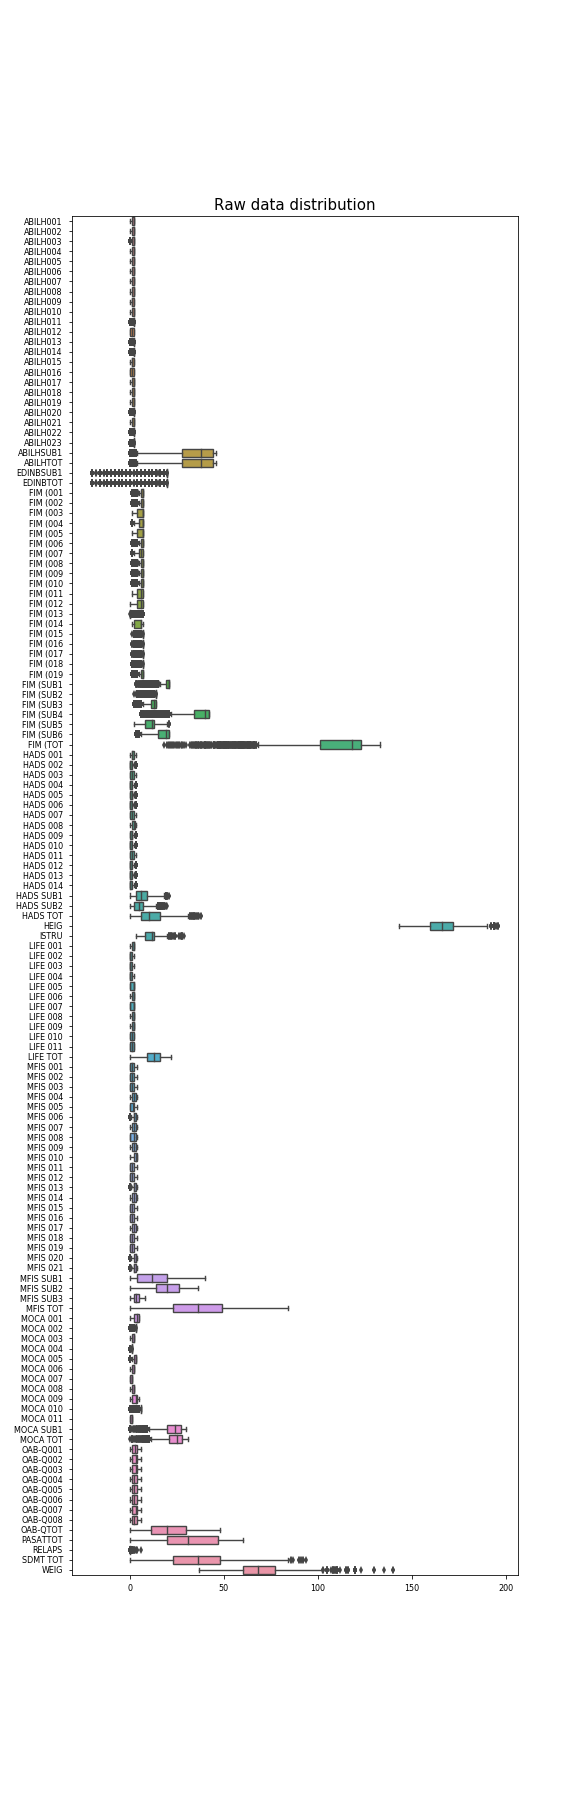
\includegraphics[trim={0 6cm 0 6cm}, width=0.5\textwidth]{part2/ms_raw_boxplot.png}
		\label{fig:ms_boxplots_pre}%
	}%
	%	\hfill%
	\subfloat[]{%
		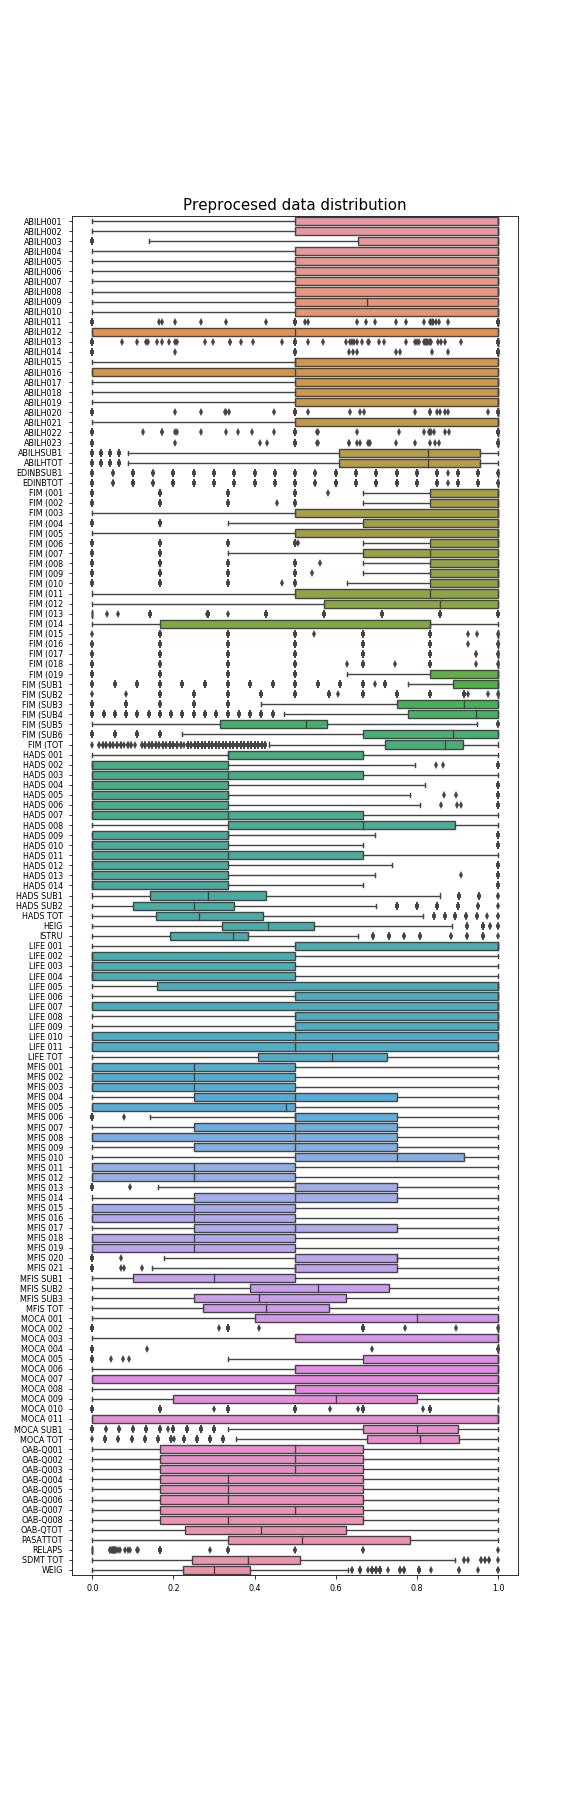
\includegraphics[trim={0 6cm 0 6cm}, width=0.5\textwidth]{part2/ms_mm_boxplot.png} \label{fig:ms_boxplots_post}
	}%
	\caption{The effect of the data preprocessing on the input ordinal \PCOs. The left panel (a) shows the distribution of the raw collected variables, whereas the right panel (b) shows the distribution of the same variables after the preprocessing step.}\label{fig:ms_boxplots}
\end{figure}

Furthermore, we try to decrease the dimensionality of the collected samples in order to visually inspect the data. To this aim, we project the data in a 3D space with linear PCA and Isomap (see Section~\ref{sec:dimred}).
These algorithms are sensitive to outliers, which we expect to affect our dataset. Therefore, we follow a preliminary isolation forests-based anomalies detection and removal as described in~\cite{liu2008isolation, liu2012isolation}.
The obtained scatter plots are shown in Figure~\ref{fig:ms_3dscatterplot}.
As we can see, both the obtained projections hint some sort of class separation between \RR and \SP subjects, while the same conclusion cannot be drawn for the other classes. Moreover, considering only the first three principal components, PCA explains only the $37.4\%$ of the variance of the dataset. This suggests that more information, which may be useful for classification purposes, is spread across several input variables.
%in this dataset the low dimensionality projection and visualization is not insightful. From the scatter plots in Figure~\ref{fig:ms_3dscatterplot} a clear class separation cannot be firmly observed.

\begin{figure}[h!]
	\centering
	\subfloat[]{%
		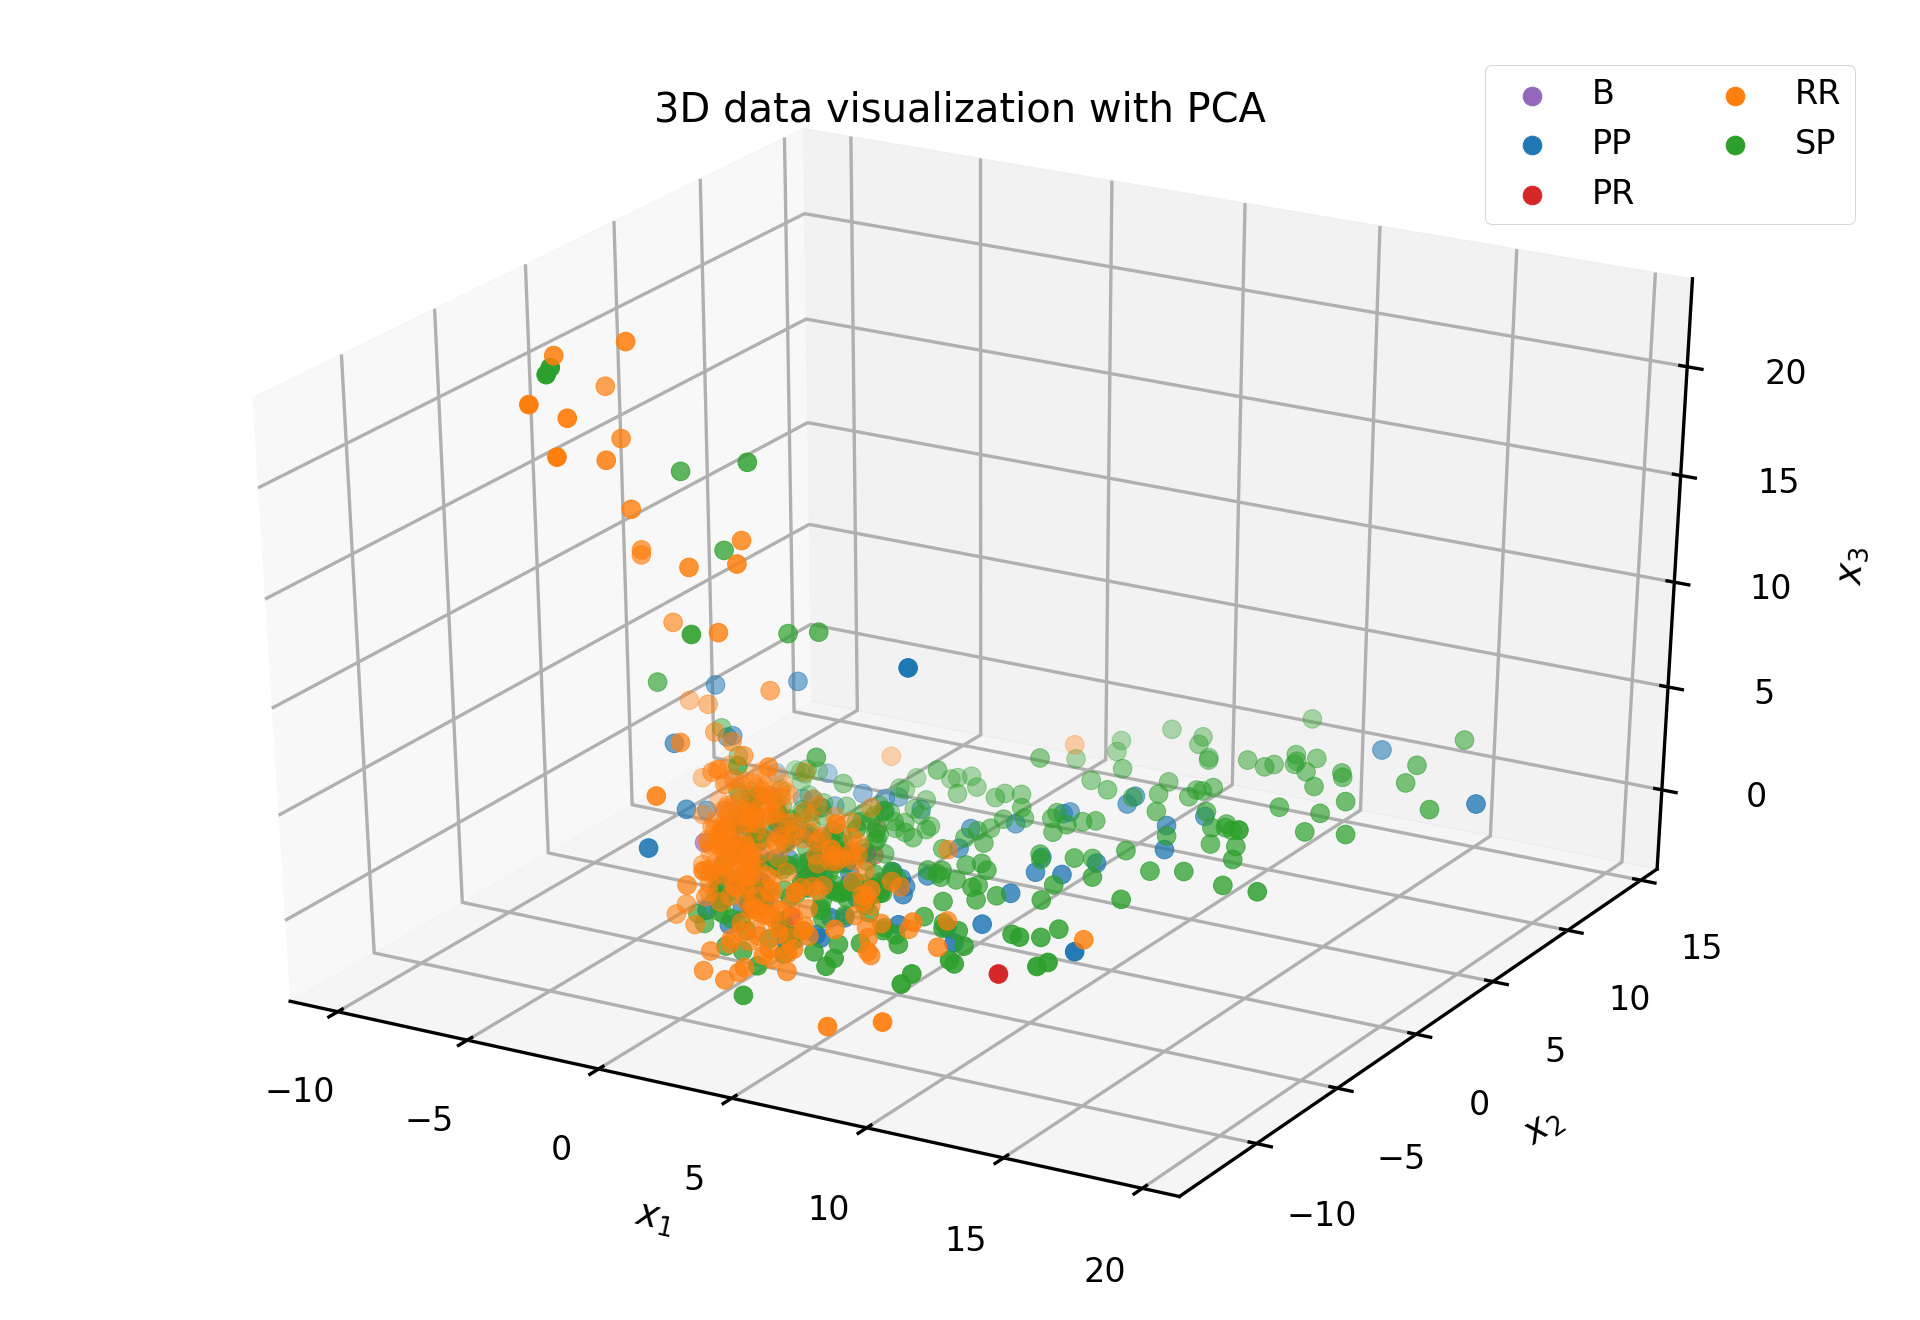
\includegraphics[width=0.5\textwidth]{part2/ms_pca.png}
		\label{fig:ms_ms_pca}%
	}%
%	\hfill
	\subfloat[]{%
		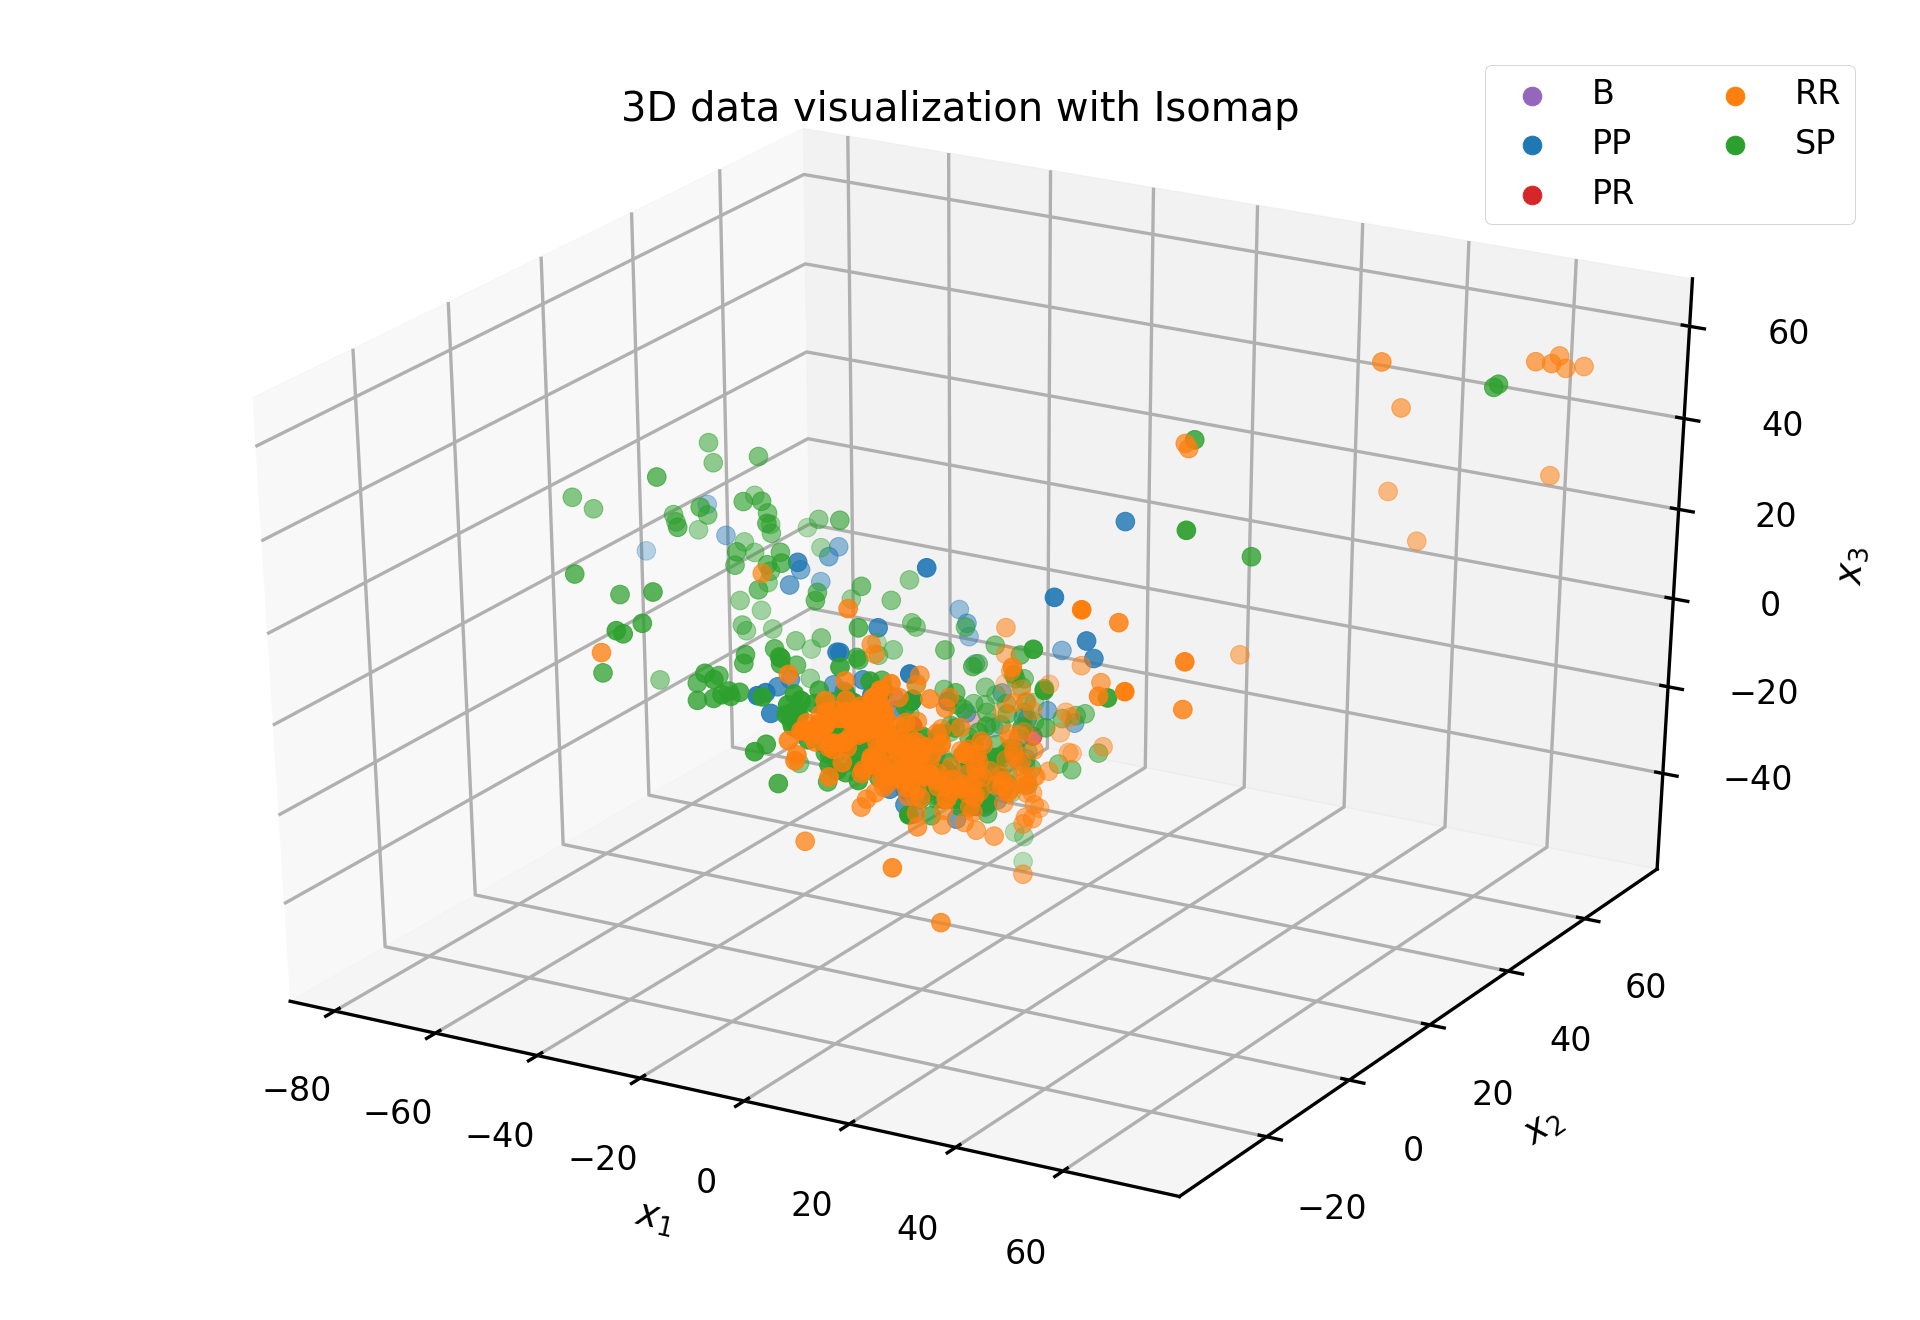
\includegraphics[width=0.5\textwidth]{part2/ms_isomap.png}
		\label{fig:ms_ms_isomap}%
	}
%	\subfloat[]{%
%		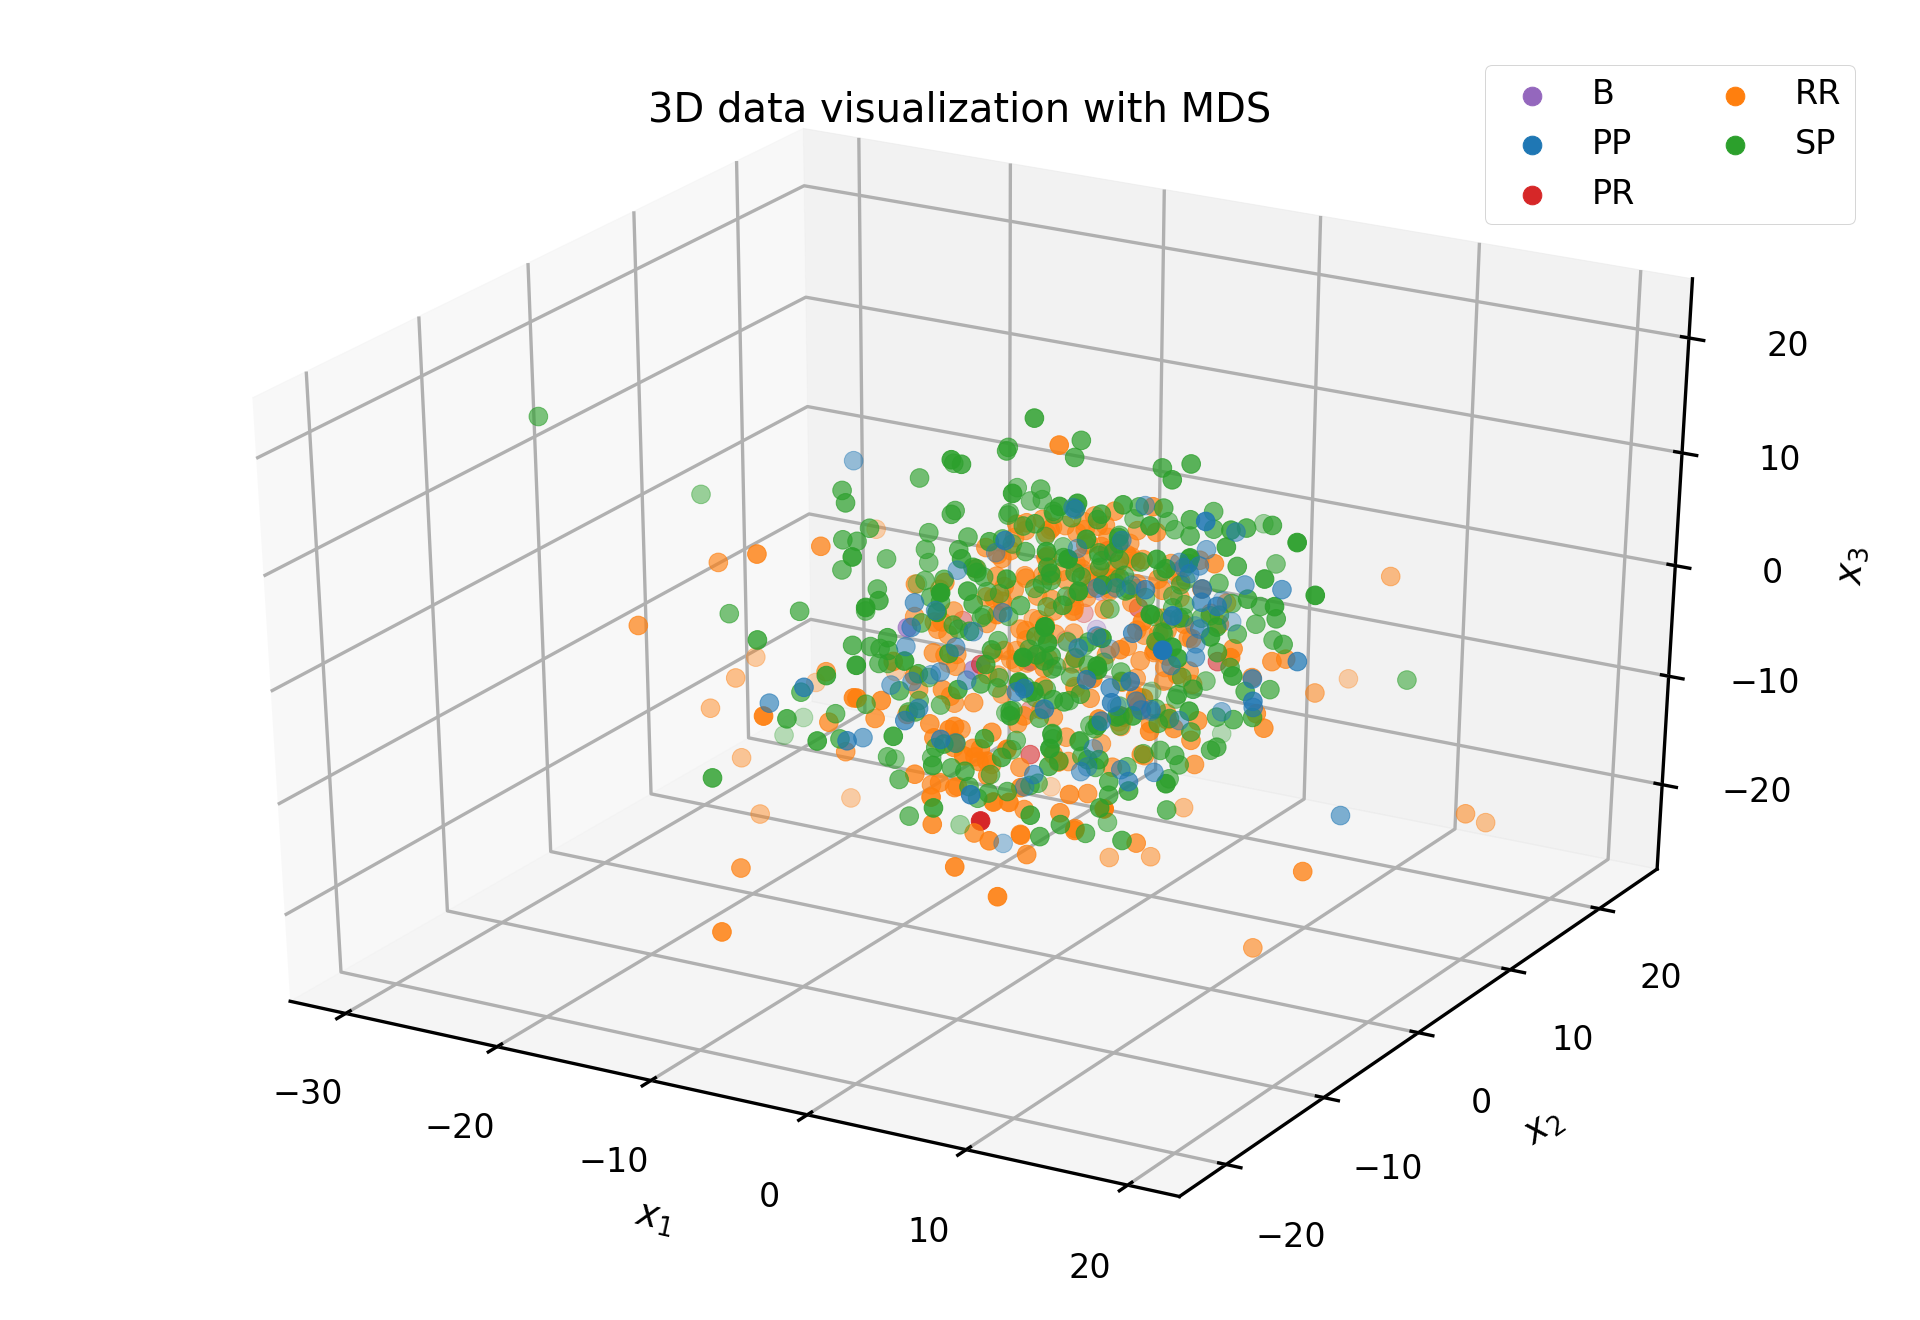
\includegraphics[width=0.5\textwidth]{part2/ms_mds.png}
%		\label{fig:ms_ms_mds}%
%	}%
%	\subfloat[]{%
%		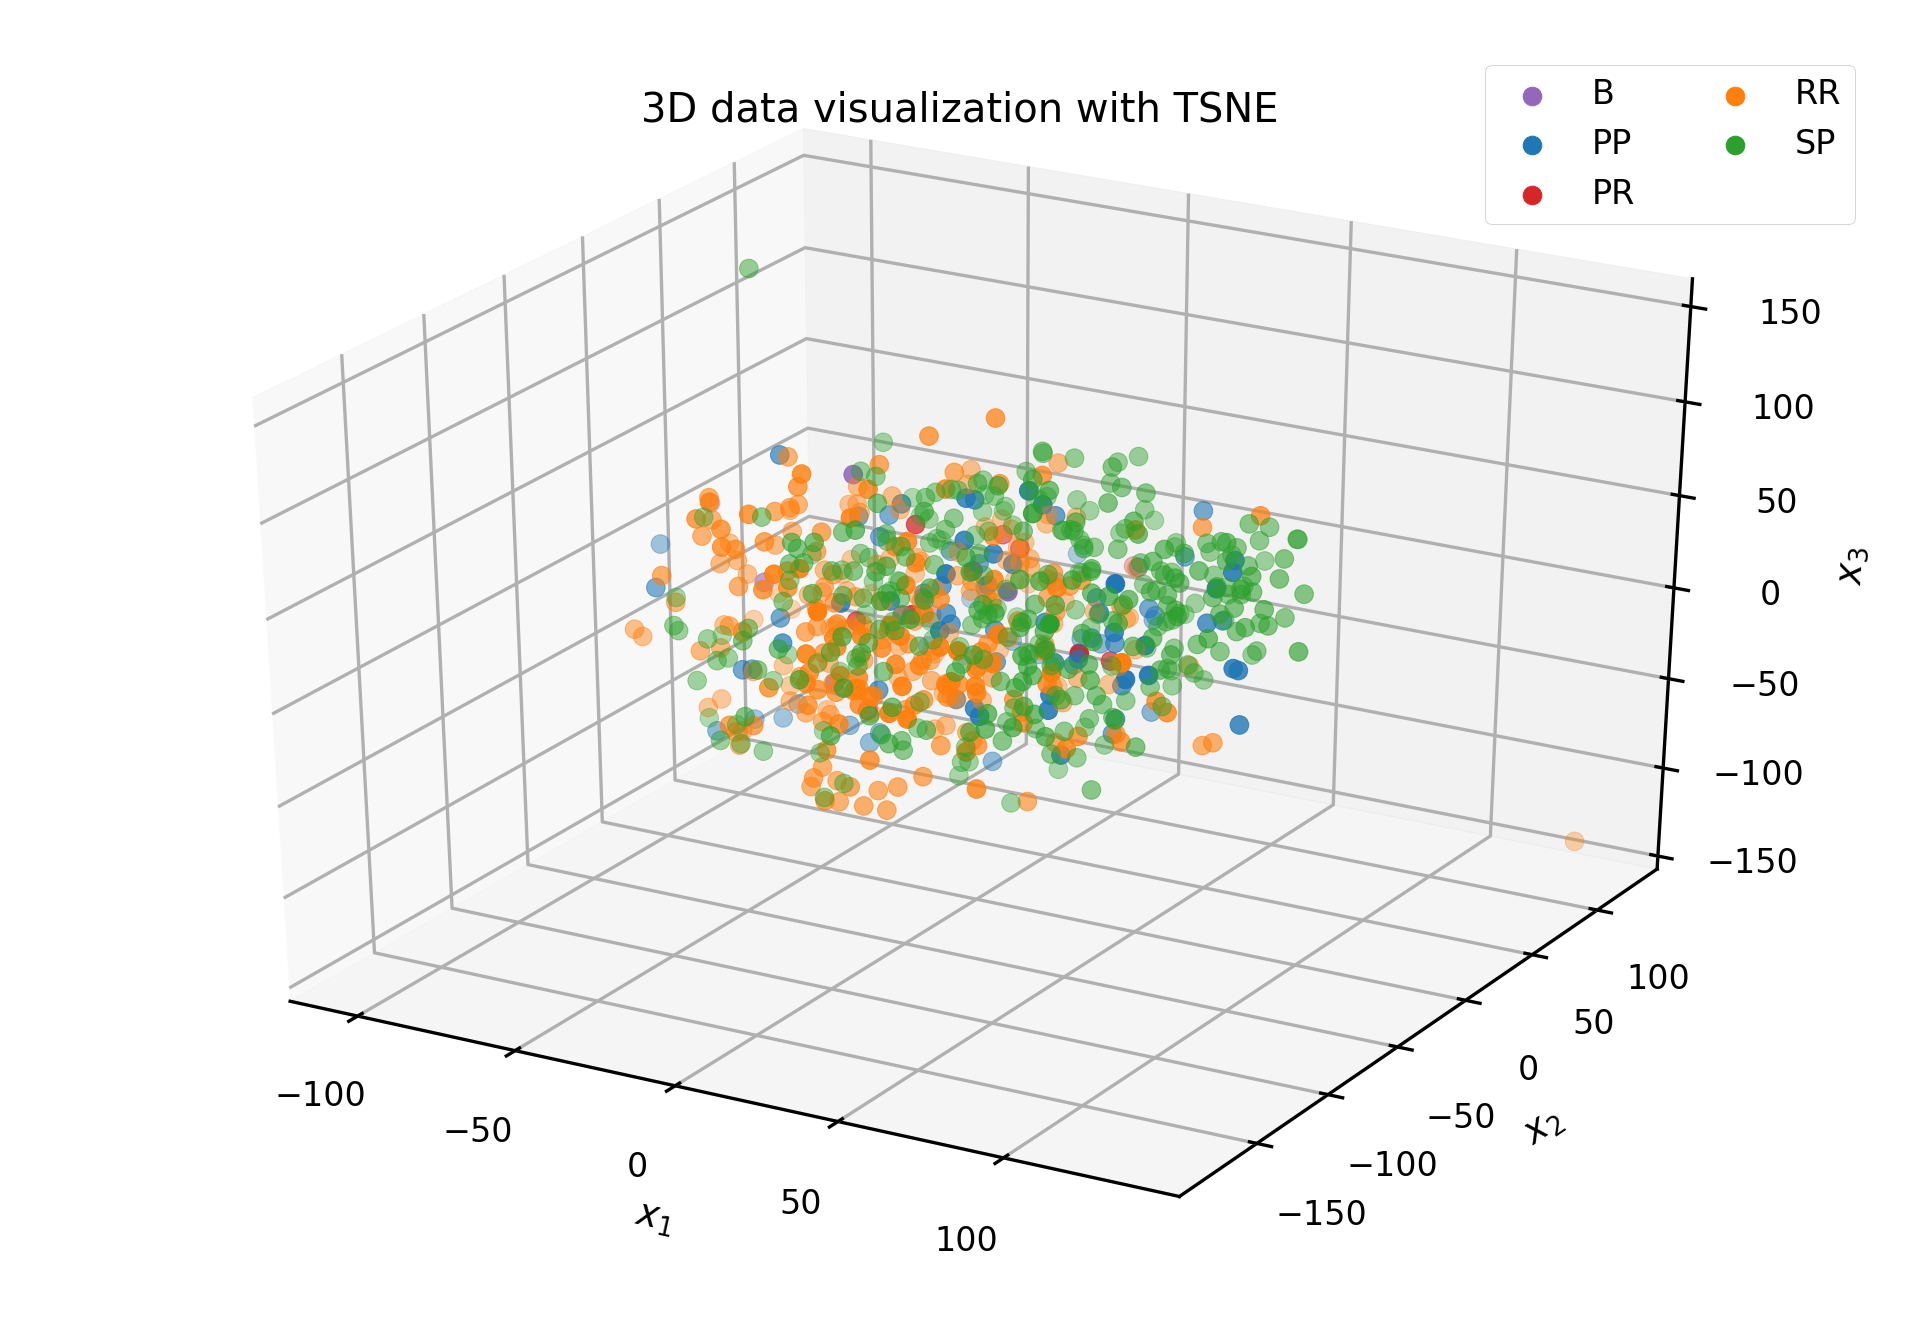
\includegraphics[width=0.5\textwidth]{part2/ms_tsne.png}
%		\label{fig:ms_ms_tsne}%
%	}
	\caption{A random extraction of the $20\%$ of the MS dataset projected on a 3D space by linear PCA, panel (a), and Isomap, panel (b).} \label{fig:ms_3dscatterplot}
\end{figure}

This EDA raised our hopes to successfully perform a further supervised MS course classification and evolution prediction.

% The number of considered samples across examinations is hence $2699$, of which $1220$ \RR and $1579$ \SP.


\section{Supervised analysis}\label{sec:problem_description}

% We adopted suitable categorical data encoding and missing values imputing strategies to cope with these issues (see Section~\ref{sec:problem_description}).

%a machine-learning based temporal model that, extracting information from \PCOs data, is able to answer to
Predicting the MS course evolution can be split in three different related tasks: \f (\F), \g (\G) and \fog (\FOG).

\begin{enumerate}
	\item[] \textbf{\F} Given the $165$-dimensional representation of a patient at a fixed time point $\bm{x}_i^t$, this task consists in assigning the corresponding disease course $y_i^t$. \F can be translated into a binary classification problem and which can be solved by learning a discriminative function $f(\bm{x}_i^{t}) = y_i^{t}$.
	
	\item[] \textbf{\G} Given the historical representation  of a patient $\bm{x}_i^t$ for $t=1,\dots,\tau$, this task consists in predicting the patient representation $\bm{x}_i^{\tau+1}$. \G can be seen as a multiple-output regression function and it can be solved by learning an appropriate function $g(\bm{x}_i^{t}) = \bm{x}_i^{t+1}$.
	
	\item[] \textbf{\FOG} This task can be seen as foreseeing the MS disease course $y_i^{\tau+1}$ from $\bm{x}_i^t$ for $t=1,\dots,\tau$. Once $\hat{f}(\bm{x})$ and $\hat{g}(\bm{x})$ are learned by training on historical \PCO data, the \FOG problem is finally solved by the temporal model $\hat{f} \circ \hat{g}(\bm{x}_i^{t}) = y_i^{t+1}$. In time-series data analysis, this is known as \textit{one-step-ahead forecast}. Notably, the \FOG model allows to foresee if the patient at the next time point is going to experience a transition from \RR to \SP, or not.

\end{enumerate}

All these predictive models assume the temporal structure outlined in Figure~\ref{fig:pipeline}.

% documentclass[letter,10pt]{article}
% \usepackage{amsmath}
% \begin{document}

\begin{figure}[]
  \centering
  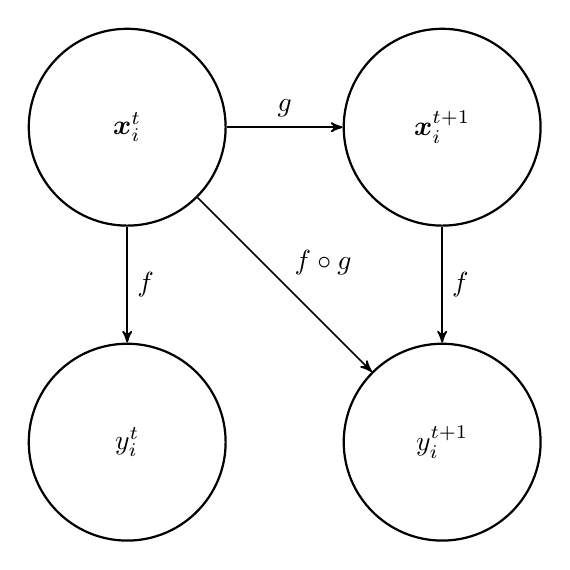
\begin{tikzpicture}[->, >=stealth', auto, semithick, node distance=4cm]
    \tikzstyle{every state}=[fill=white,draw=black,thick,text=black,scale=1, minimum height=2.5cm]
    \node[state]    (xit)                     {$\bm{x}_i^t$};
    \node[state]    (yit)[below of=xit]       {$y_i^t$};
    \node[state]    (xit1)[right of=xit]      {$\bm{x}_i^{t+1}$};
    \node[state]    (yit1)[below of=xit1]     {$y_i^{t+1}$};
    \path
    (xit)  edge node{$f$} (yit)
    (xit)  edge node{$g$} (xit1)
    (xit1) edge node{$f$} (yit1)
    (xit)  edge node{$f\circ g$} (yit1);
  \end{tikzpicture}
  \caption{A visual representation of the temporal structure assumed in the collected data. When the two functions $f$ (\F) and $g$ (\G) are learned, the \FOG model $f\circ g$ is able to predict the evolution of the disease course for future time points $y_i^{t+1}$.}\label{fig:pipeline}
\end{figure}
% \end{document}



\subsection{Experimental design}\label{sec:experimental_design}
Our final goal is predicting MS course evolution of  \RR and  \SP patients, hence the subjects with \PR, \PP and benign forms are not further taken into account.

We considered all the patients with a minimum of $1$ time point (the most recently enrolled) up to $T=11$ time points for a total of $3398$ samples, of which $1451$ \RR and $1947$ \SP. As this is an ongoing project, the number of PwMS decreases with time.
%We expect to fill the gap of samples between \textit{Exam~$1$} and \textit{Exam~$11$} by the end of the funded study.

Following the EDA, we opted for a preliminary feature-wise min-max scaling.
However, to promote unbiasedness on the results, this preprocessing phase is not performed on the entire data collection, but it is embedded into the model fitting procedure.
%separately evaluated prior to each model fitting process on its training cross-validation portion of the data.


We shall discuss separately the experimental designs used to learn $f(\bm{x})$ and $g(\bm{x})$.

% In particular, the training set comprises all samples collected at time points $t = 1, \dots ,T_{tr}$, the validation set at $t=T_{tr}+1,\dots,T_{vld}$ and the test set at $t=T_{vld}+1,\dots,T$.
% Here, as the maximum number of collected time points is $T=8$, we fixed $T_{tr} = 3$ and $T_{vld} = 4$.
% In particular, the training set comprises all samples collected at time points $t = 1, \dots ,T_{tr}$, the validation set at $t=T_{tr}+1,\dots,T_{vld}$ and the test set at $t=T_{vld}+1,\dots,T$.

\begin{itemize}
	\item[] \textbf{\F} The \F model $f(\bm{x})$ solves a binary classification problem: to each input $\bm{x}_i^t$ is associated  an output $y_i^t$ that encodes the corresponding MS disease course (\RR or \SP) with a binary label.
	We split the dataset in three temporal chunks, namely \textit{training}, \textit{validation} and \textit{test} sets, consisting of all samples collected at time points $t=1,2,3$, $t=4$ and $t=5,6,7,8,9,10,11$, respectively.
	Accordingly, we used $1993$ samples for training $f(\bm{x})$, $463$ for validation leaving the remaining $942$ for test.
	
	Five candidate models for $f(\bm{x})$ are fitted on $100$ Monte Carlo (MC) random sampling of the training set each time keeping $\frac{1}{4}$ of the samples aside~\cite{molinaro2005prediction}. For each MC sampling the fitting procedure is performed on the remaining $\frac{3}{4}$ of the samples and it includes an inner parameter optimization via grid-search cross-validation~\cite{hastie2009elements}. In particular, we require the MS course prediction to be based on a reduced number of variables (see Section~\ref{sec:learning_f}), therefore we enforce sparsity in each candidate model.
	% Each candidate model is required to be sparse, therefore the MS course prediction is based on a reduced number of variables (see Section~\ref{sec:learning_f}).
	Leveraging on the MC strategy, we rank the variables according to their selection frequency~\cite{barbieri16palladio, meinshausen2010stability}.
	Once a variable ranking is achieved for each candidate model, the list of selected variables is identified by thresholding the corresponding ranking with the threshold that maximizes the accuracy \todo{or MCC} on the validation set. Finally, the last training step consists in fitting each candidate model on the union of training and validation sets taking only into account the corresponding reduced subset of selected variables. The final \F model $\hat{f}(\bm{x})$ is chosen as the one that performs better on the previously unseen test set in terms of accuracy, \todo{MCC}, precision, recall and $\text{F}_1$ score.

	\item[] \textbf{\G} %presents the answers provided by the MS patients to the \PCOs questionnaires, while the label vector $\bm{y}$ has the corresponding disease form diagnosis.
	On the other hand, learning the \G model $g(\bm{x})$ implies solving a multiple-output regression problem and each input $\bm{x}_i^t$ is associated with the output vector $\bm{x}_i^{t+1}$.
	% and the class labels are not taken into account.
	Therefore, we can only consider samples at time point $t$ with an available follow-up at the next time point $t+1$, which reduces the overall number of available samples.
	The dataset splitting is consistent with the one followed for learning $f(\bm{x})$, although there is no need for a separate validation set, as learning $g(\bm{x})$ does not require any variable selection process. We used the samples collected at time points $t=1,2,3$ for training and those at $t=4,5,6,7,8,9,10,11$ for test, resulting in $XXXX$ and $XXX$ samples, respectively.
	The fitting procedure includes an inner parameter optimization via grid-search cross-validation. Each candidate model is a function
	$g: \mathbb{R}^{165} \rightarrow \mathbb{R}^k$ where $k$ is the number of variables selected by the best \F model.
	% that predicts the evolution of the variables selected by the best \F model starting from the full set of \PCOs.
	The final \G model $\hat{g}(\bm{x})$ is chosen as the candidate model that performs better on the previously unseen test set in terms of mean absolute error (MAE).
	

	\item[] \textbf{\FOG} The predictive capability of the \FOG model $\hat{f} \circ \hat{g}(\bm{x})$ is finally evaluated on the test set. The \F model $\hat{f}(\bm{x}_i^t)$ predicts the MS course $\hat{y}_i^t$ from the \PCO data vector $\hat{\bm{x}}_i^t$ that, in turn, is predicted by the \G model $\hat{g}(\bm{x}_i^{t-1})$. We shall notice here that the predictions $\hat{f} \circ \hat{g}(\bm{x}_i^t)=y_i^{t+1}$ for $t=11$ are foreseeing possible \RR to \SP transitions that are beyond our data observation, hence predictions at the last time point cannot be used to assess the \FOG model performance. Therefore, its performance is evaluated only on $XXXX$ test samples.
	
\end{itemize}




%Finally, the predictive capability of the prognosis model $\hat{f} \circ \hat{g}(\bm{x})$ is evaluated by predicting $\hat{g}(X_{T-1})=\hat{X}_T$, that is the evolution of the \PCOs for the patients at time point $T-1$, then applying the diagnosis model on the predicted data matrix $\hat{f}(\hat{X}_T)=\hat{y}_T$ and comparing them with the diagnosis provided by the doctors at the same examination.



\subsection{Learning $f(x)$} \label{sec:learning_f}


%First, we will require the diagnosis function $f(\bm{x})$ to be sparse, hence the MS outcome prediction will be based on a reduced number of variables.
We imposed $f(\bm{x})$ to be sparse. This requirement is helpful from two distinct respects:
\begin{enumerate*}[label=\alph*)]
	\item the performance of the predictive model may increase thanks to a reduced effect the course of dimensionality~\cite{hastie2015statistical} and
	% \item the effect the course of dimensionality~\cite{hastie2015statistical} may be attenuated, hence increasing the performance of the predictive model, and
	\item the identification of a reduced subset of meaningful \PCOs provides interpretability of the results for the clinicians.
\end{enumerate*}
In order to achieve such sparse model, we take advantage of two main variable selection strategies: embedded and wrapper methods~\cite{guyon2003introduction}.
When using embedded methods, we exploited the sparsity inducing penalties of EN to take into account possible correlation between \PCO variables and of SLR to benefit from the renowned classification capability of the logistic loss function.
We applied the RFE wrapper method to
% Concerning the use of wrapper methods, which exploit a RFE schema, we chose
two tree-based learning machines (RF and GB) that are capable of capturing nonlinear relationship between input and output and are intrinsically well-suited to deal with categorical/ordinal variables. We also explored the use of RFE with SVM, as in~\cite{guyon2002gene}.
% which is a state-of-the-art machine learning method for classification.

\subsection{Learning $g(x)$}

As no prior information on the relationship between \PCOs evaluated at different time points was available, to learn $g(\bm{x})$ we investigated on the use of both linear and nonlinear models.
% To learn $g(\bm{x})$ no prior information on the relationship between \PCOs evaluated at different time points was available. To achieve our goal, we investigated on the use of both linear and nonlinear models.

Concerning the linear models, we explored two different solutions: NNM and MTEN. The first imposes a low-rank prior on the result. The second is a natural multiple-output extension of EN, hence it induces a row-structured sparsity pattern on the solution where collinear variables are more likely to be included in the model together. For nonlinear prediction, we resorted to the state-of-the-art MLP approach.

\section{Results}\label{sec:results}

% \todo{add table of selected features}
We shall discuss separately the results achieved in terms of \F, \G and \FOG models.

Regarding \F, the GB method outperforms the other candidate models reaching accuracy $0.900$, precision $0.936$, recall $0.899$ and $\text{F}_1$ score $0.917$, as shown in Figure~\ref{fig:diagnosis_competition}. Therefore we chose it as \F model $\hat{f}(\bm{x})$.
Insights on the use of \PCOs for MS assessment are provided by the sparsity of the \F model induced by the RFE schema.
The $31$ selected variables are reported in Table~\ref{tab:selected}.
Comparing the full list of \PCO questionnaires of Table~\ref{tab:proms} with Table~\ref{tab:selected}, we observe that each \PCO used in this study is represented at least once, except \EDINB, and the most represented is \FIM.
We also see that, whenever possible, the model tends to select aggregate scores (total and subtotal) rather that single items. This is consistent with the clinical practice, where neurologists are more likely to assess patient's health status by using the aggregate scores, rather than the single questions.
Quite surprisingly, the recent number of relapses is the only additional information not selected by the model.
Finally, we note that all the domains that are known to be affected by the disease are well covered: mobility (upper and lower limbs), cognition, emotional, fatigue, bladder and psychosocial.
The heatmap in Figure~\ref{fig:selection_heatmap} shows the Hamming distance estimated across the list of variables selected by the five \F candidate models. Interestingly, tree-based methods are more prone to select similar variables with respect to linear methods. As expected, the sparsity induced by the $\ell_1$-norm of SLR allows the method to achieve a list of variables similar to the one obtained by SVM-RFE, while the list obtained by ENET includes collinear variables and it is significantly different from the others.

Regarding \G, MTEN outperforms the other candidate models in terms of MAE ( $\text{MAE}_{\text{MTEN}}=0.095$, $\text{MAE}_{\text{NNM}}=0.102$, $\text{MAE}_{\text{MLP}}=0.105$), hence we select it as our \G model $\hat{g}(\bm{x})$.


 \begin{figure}[h!]
	\centering
	\subfloat[]{%
		\includegraphics[width=0.5\textwidth]{part2/final_scores_2_copy.png}
		\label{fig:diagnosis_competition}%
	}%
	 \hfill%
	\subfloat[]{%
		\includegraphics[width=0.5\textwidth]{part2/selection_heatmap_copy.png} \label{fig:selection_heatmap}
	}%
	\caption{A visual representation of the results obtained from the \F model. On the left panel (a) we show the classification performance achieved on the test set by the candidate models. Precision, recall and $\text{F}_1$ score are estimated considering \SP as the positive class. As GB outperforms the other methods on each performance metric, it is chosen as \F model. On the right panel (b) a heatmap displays the distance between the lists of variables selected by each model in terms of their hamming distance. \todo{break figure in two}}\label{fig:f}
\end{figure}


%
Finally, the \FOG model $\hat{f} \circ \hat{g}(\bm{x})$, obtained by combining MTEN and GB achieves the following performance scores on the $220$ test samples: accuracy $0.841$, precision $0.900$, recall $0.824$ and $\text{F}_1$ score $0.860$.


\section{Conclusions and future works}

This chapter describes a temporal model based on \PCOs and ML for disease form prediction in MS.
In particular, we address the tasks of current course assignment, \PCOs evolution prediction and future course assignment. The model is built on a collection of \PCOs acquired on a cohort of individuals enrolled in an ongoing funded study (\textit{DETECT-MS PRO}).

% The measures are categorical or ordinal answers to a given set of \PCOs.
\PCOs data are typically used to corroborate evidence provided by quantitative exams, in our case the absence of clear MS disease form predictors makes the information extracted from \PCOs data the only available resource.
The proposed temporal model was able to correctly assign the current MS form and to foresee future ones with accuracy of $90.0\%$ and $84.1\%$, respectively \todo{fixme}.
This demonstrates that \PCOs can effectively be used as MS disease course predictor.
%In the next future, we plan to expand the data collection with respect to the amount of enrolled subjects as well as the number of time points.

In the next future, we plan to further investigate on the predictive capabilities of the proposed model with longer temporal horizons and to compare it with different approaches, such as probabilistic graphical models.
%, that allow to explicitly incorporate the temporal nature of the data.}

Given the achieved promising results, the proposed model is soon going to be validated in clinical practice, where it will assist the clinicians involved in this study to foresee possible disease course transition and to take important decisions concerning treatment and therapies that can substantially improve the quality of life of their patients.
% In fact, the proposed temporal model was able to correctly foresee the evolution of the disease form of $84.1\%$ of MS patients.

In the context of neurodegenerative diseases, clinicians typically use \PCOs data to corroborate evidences coming from standard quantitative exams \cite{black2013patient}. Interestingly, in our case the absence of clear \SP predictors makes the information extracted from \PCOs data the only available resource.
%Our result shows that a timely prediction of the disease course can be obtained from patient-friendly and low-cost measures.

In the era of precision medicine, the problem of predicting MS course evolution still relies on stressful exams and clinical judgement.
To the best of our knowledge, this is the first attempt to solve this delicate task leveraging only on patient-friendly measures and ML.



% !TEX root = ../main.tex

\chapter{Data-driven strategies for robust forecast of continuous glucose monitoring time-series} \label{chap:diabete}
% EMBC

\begin{displayquote}
\textit{Over the past decade, continuous glucose monitoring (CGM) has proven to be a very resourceful tool for diabetes management. To date, CGM devices are employed for both retrospective and online applications. Their use allows to better describe the patients' pathology as well as to achieve a better control  of  patients' level of glycemia. The analysis of CGM sensor data makes possible to observe a wide range of metrics, such as the glycemic variability during the day or the amount of time spent below or above certain glycemic thresholds. However, due to the high variability of the glycemic signals among sensors and individuals, CGM data analysis is a non-trivial task. Standard signal filtering solutions fall short when an appropriate model personalization is not applied. State of the art data-driven strategies for online CGM forecasting rely upon the use of recursive filters. Each time a new sample is collected, such models need to adjust their parameters in order to predict the next glycemic level. In this chapter we will see that the problem of online CGM forecasting can be successfully tackled by personalized machine learning models, that do not need to recursively update their parameters.}
\end{displayquote}

\section{Introduction: modern diabetes care}
Diabetes is a chronic metabolic disorder affecting nearly $400$ million of individuals worldwide. The number of diabetic patients is increasing and it is expected to reach almost $600$ million in the next future~\cite{guariguata2014global}.
%In the world people with type 2 diabetes are $400$ million and this  number will rise to $600$ million in $2035$~\cite{guariguata2014global}. 
%http://www.who.int/diabetes/global-report/en/
%https://www.cdc.gov/diabetes/statistics/incidence/fig2.htm
According to the {\em World Health Organization}~\cite{world2016global}, the global prevalence of diabetes among adults has nearly doubled in the last few decades, rising from $4.7\%$ in 1980 to $8.5\%$ in 2014.
%and its incidence per year is $6.9$ per $1,000$ individuals~\cite{}.
%In the western population the  prevalence of diabetes is $6$ to $10\%$ .
%The incidence of diabetes type $2$ is $5-7/1000/$year \todo{non sono sicuro di aver capito}.
If not treated correctly, diabetes may cause several permanent complications, such as visual impairment and kidney failure. 
%, that heavily affect the quality of life of the patients

Hypoglycemia is a severe risk in diabetes therapy. 
The mean incidence of hypoglycemia in patients with type $1$ diabetes (T1D) 
is 1-2 events per week, while severe hypoglicemia occurs 0.1-1.5 episodes per year~\cite{van2016continuous}. 
Moreover, hypoglycemia interferes with the quality of life and increases the risks of cardiovascular events in type $2$ diabetes (T2D) patients~\cite{van2016continuous}. On the other hand, hyperglycemia associates with an increased risk of diabetes complication as well.


The most common glucose monitoring solutions are self blood glucose meters and Continuous Glucose Monitoring systems (\ac{CGM}). 
CGM devices are minimally-invasive, and can be used in daily life for retrospective or online applications~\cite{vigersky2017role}. 
CGM systems measure interstitial glucose concentration at fixed time intervals, enabling an accurate observation of glycemic variability during the day as well as the ratio of time spent in hypo/hyperglycemia. 
When CGM is employed online, an improvement of the therapy can be achieved by embedding in the system a tool that foresees glucose levels using suitable time-series models trained on past  CGM  data~\cite{sparacino2007glucose}. In this case, alarms can be generated when the glucose concentration exceeds the normal range~\cite{vigersky2017role}.
%thresholds

%Such tools implement algorithms to foresee hypo/hyperglycemic  events that can be obtained  by  generating alerts on  the basis of future glucose level forecast by  using  past  CGM  data  and  suitable time-series  models \cite{sparacino2007glucose}.
%\cite{monnier2016near}
%\todo{
%State-of-the-art in diabetes monitoring is glycemia self assessment via glucose meters~\cite{monnier2016near} NON SONO SICURO DELLA REF},   it is possible to self-manage diabetes with continuous glucose monitoring (CGM) devices. CGM systems measure interstitial glucose concentration at fixed time intervals (e.g., each $5$ minutes). 
%
%CGM enables the observation of glycemic variability during the day as well as the ratio of time spent in hypo/hyperglycemia. 
%
%
%These devices are minimally-invasive, and can be used in daily life, but, to date, they are mainly used for retrospective and online applications~\cite{vigersky2017role}. 
%
%In both cases, CGM enables the observation of glycemic variability during the day as well as the ratio of time spent in hypo/hyperglycemia. 
%
%When CGM is employed online, an improvement of the therapy can be achieved by embedding in the system a tool able to generate alerts when the glucose concentration exceeds the normal range thresholds~\cite{vigersky2017role}, based on past  CGM  data  and  suitable time-series  models \cite{sparacino2007glucose}.

%In many clinical situations


To model patient-specific Blood Glucose (BG) levels, several approaches, integrating various information, were proposed~\cite{bunescu2013blood, zecchin2011new}. However, the problem of glycemic level prediction is still challenging, due to the high CGM signal variability among patients and acquisition devices.

This chapter describes the third, and last, biomedical data science challenge of the thesis. Throughout this chapter we assume that CGM signals have structural information on time-changes of BG concentration \cite{sparacino2007glucose, bunescu2013blood} and we perform glycemic level forecasting exploring the performance of a set of purely data-driven techniques for time-series analysis.

Data-driven forecasting approaches, as opposed to models driven by an \textit{a-priori} description of the underlying phenomena, are capable of modeling input/output relationships without requiring prior knowledge on the field of use. This family of approaches can be successfully employed to obtain reliable predictions without modeling complex, and possibly not completely understood, environments. Data-driven forecasting models are widely applied in  real-world scenarios often employing a moving-window paradigm, \ie the system keeps track of the last $w$ acquisitions using them to forecast future values.

In this chapter, we focus on two main groups of data-driven methods for online time-series forecasting: \textit{recursive filters} and, of course, ML models.
The first group includes linear stationary models, such as Autoregressive Moving Average (\ac{ARMA}), non stationary models, such as Autoregressive Integrated Moving Average (\ac{ARIMA}) and adaptive filtering techniques, such as the Kalman Filter (\ac{KF}). These methods are well-established and extensively used, but they require recursive parameters adjustment for every new collected sample \cite{box2015time}.
As these methods are note covered in Chapter~\ref{chap:state-of-the-art}, a quick overview is provided in Section~\ref{sec:recursive_filters}. 

The second group comprises regularized kernel methods, such as Kernel Ridge Regression (\ac{KRR}) (see Sections~\ref{sec:ridge_regression} and~\ref{sec:kernel_trick}) and deep learning methods, such as Long Short-Term Memory networks (\ac{LSTM}), see Section~\ref{sec:lstm}.

As we have seen in the previous chapters, ML methods showed very promising results in several applications, also including time-series forecasting \cite{bunescu2013blood, schmidhuber2005evolino}. To achieve a predictive model, they need to learn the model parameters from a training set. This learning process is done \textit{only once} and it conveys a model that does not require further parameter adjustments to predict future values. This remarkable advantage makes machine learning models more suitable to be delivered on embedded portable systems.

This chapter aims at understanding whether purely data-driven machine learning methods can be successfully employed to forecast glucose values of diabetic patients.  

\section{Temporal forecasting problem setting}

%\todo{aggiustare il tiro qui}
%In this study we aim at comparing four different data-driven models
% for online CGM sensor data {\em forecasting}: {\em Auto Regressive Integrated Moving Average} (ARIMA) , {\em Kalman Filter} (KF), {\em Kernel Ridge Regression} (KRR) and {\em Long Short-Term Memory} (LSTM) {\em Network}.
In the previous chapters we fixed the notation for regression and classification problems. The temporal forecasting can be seen as a special regression case, therefore some additional notation is needed.

Given a set of data $\mathcal{S}$, we refer to data-driven models with hyperparameters $\bm{\theta}$ as $\mathcal{M}_\mathcal{S}(\bm{\theta})$.
%Given $y_i(t)$, the time-series associated with the $i$-th subject, for $t=t_k,\dots,t_{k+w}$ we aim at predicting $y_i(t_{k+w}+\Delta T)$, where $\Delta T$ is some prediction horizon.
Given the time-series $y(t)$ we aim at predicting $y(t+\Delta T)$, where $\Delta T$ is some {\em prediction~horizon}.

A well-known issue of CGM sensor data analysis is that signal properties, such as the signal-to-noise ratio, may vary among devices and individuals~\cite{facchinetti2010online}. In order to achieve an accurate forecast of the glucose level of a given individual from past samples, any prediction model $\mathcal{M}_\mathcal{S}(\bm{\theta})$ must be \textit{personalized}. Such model personalization procedure is two-fold: \textit{hyperparameters }($\bm{\theta}$) \textit{optimization}, also known as model selection (see Section~\ref{subsec:model_selection}), and {\em parameter estimation}, or model fitting. 
In this work we fixed a common strategy for hyperparameters optimization whilst the actual model fitting procedure is defined differently according to the model. 
%(i.e., $25$ hours at 5 minutes sampling period)(in our dataset, this set lasted up to $6$ days)

\section{Recursive filters overview} \label{sec:recursive_filters}
Recursive filters are the most widely adopted class of temporal forecasting strategies.
In this chapter we make CGM temporal prediction by exploiting two different recursive filters approaches: ARIMA and KF. Providing a comprehensive overview of temporal forecasting strategies is beyond the scope of this thesis, therefore Chapter~\ref{chap:state-of-the-art} does not cover this topic. This section sketches the main ideas behind this two strategies, providing the information that are necessary to understand this last biomedical data science challenge.

\subsection{Autoregressive Integrated Moving Average}
ARIMA methods can be used to perform linear forecasting of non stationary time-series assuming that its $d$-th difference is a stationary ARMA process  \cite{box2015time}. The output of an ARMA process, with white input noise $u(t)\sim\mathcal{N}(0,\sigma^2)$, can be expressed as in Equation~\eqref{eq:arma}.
\begin{equation} \label{eq:arma}
y(t) = -\sum_{k=1}^pa_ky(t-k)+\sum_{k=0}^qb_ku(t-k)
\end{equation}
The output of an ARMA$(p, q)$ model can be seen as the sum of $p$ autoregressive and $q$ moving average terms. This strategy requires the modeled processes to be stationary. On the other hand, when a time-series can be considered stationary after $d$ differentiations, ARIMA$(p, d, q)$ models can be used. 
This is the case for non stationary time-series that exhibit local stationary behavior. In general,  $(p, d, q)$ are unknown and we will consider them as hyperparameters of the ARIMA model.

The cross-validation index (see Section~\ref{sec:diabete_expdesign}) for ARIMA models can be defined as $J(\bm{\theta})= \text{AIC}(\mathcal{M}_{\mathcal{S}}(\bm{\theta})) + \bar{\varepsilon}_{\text{cv}}$, where AIC stands for Akaike Information Criterion~ \cite{box2015time} and $\bar{\varepsilon}_{\text{cv}}$ is the MSE evaluated via cross-validation, see Section~\ref{sec:performance_metrics}. We refer to~\cite{box2015time} for a detailed description of ARIMA model fitting.

The application of this class of models to predict CGM sensor data was also explored in \cite{sparacino2007glucose,bunescu2013blood}.

\subsection{Kalman Filter}
%\begin{equation}\label{eq:kfx}
%x(t+1) = Fx(t) + w(t)
%\end{equation}
%with measurements $y \in \mathbb{R}^k$,
%\begin{equation}\label{eq:kfy}
%y(t) = Hx(t)+v(t)
%\end{equation}


The KF addresses the problem of estimating the state $\bm{x} \in \mathbb{R}^d$ of a discrete-time process governed by the linear stochastic difference equation
$\bm{x}(t+1) = F\bm{x}(t) + \bm{w}(t)$
with measurements $\bm{y} \in \mathbb{R}^k$,
$\bm{y}(t) = H\bm{x}(t)+\bm{v}(t)$,
where $\bm{w}(t)$ and $\bm{v}(t)$ are independent random variables representing state and measurement noise, respectively \cite{welch1995introduction}. It is usually assumed that $\bm{w}(t)\sim \mathcal{N}(\bm{0}, Q)$ and $\bm{v}(t)\sim \mathcal{N}(\bm{0}, R)$, with both $Q$ and $R$ unknown. In the context of CGM sensor data prediction, we can safely assume that the state space is two-dimensional, hence $x_1(t)=u(t)$, $x_2(t)=u(t-1)$ where the unknown signal $u(t)$ is described {\em a-priori} as an integrated random-walk $u(t)=2u(t-1)-u(t-2)+w(t)$ as in \cite{facchinetti2010online}. Consequently, the state space transition matrix $F$ can be written as
%$$F=[\begin{smallmatrix}  2 & -1  \\  1 & 0\end{smallmatrix}]$,
\begin{equation}\label{eq:F}
F=
\begin{bmatrix}
2 & -1  \\
1 & 0
\end{bmatrix}
\end{equation}
while the measurement vector is
$$
H =
\begin{bmatrix} 1 & 0
\end{bmatrix}
$$
the process noise covariance is
%$Q=
%[\begin{smallmatrix}
%\lambda^2 & 0  \\
%0 & 0
%\end{smallmatrix}
%]$
\begin{equation}\label{eq:Q}
Q=
\begin{bmatrix}
\lambda^2 & 0  \\
0 & 0
\end{bmatrix}
\end{equation}
and the measurement noise covariance is $R = \sigma^2$, as in \cite{facchinetti2010online}. Both $\lambda^2$ and $\sigma^2$ are unknown and we will consider them as hyperparameters of the KF forecasting strategy.

In this case, the cross-validation index (see Section~\ref{sec:diabete_expdesign}) can be defined as $J(\bm{\theta})= \bar{\varepsilon}_{\text{cv}}$.

The application of KF to predict CGM sensor data was also explored in \cite{facchinetti2010online, knobbe2005extended}.

\section{CGM data collection}
%{\color{red}We collected samples from 178 type 1 and type 2 diabetes patients were monitored for about 1 to 7 days in  free living conditions.
%Patients wore the iPro\textsuperscript{\footnotesize \textregistered}2 Professional CGM (Medtronic), which reported glucose values every 5 minutes}.\\
%

%Patients wore the iPro\textsuperscript{\footnotesize \textregistered}2 Professional CGM sensor (Medtronic), which reported glucose values every 5 minutes.

We acquired CGM samples from a group of 148 T1D and T2D patients wearing the iPro\textsuperscript{\footnotesize \textregistered}2 Professional CGM sensor (Medtronic), which reported glucose values every 5 minutes. Patients were monitored for up to 7 days in  free living conditions, keeping track of their treatments. %, as in Figure~\ref{fig:cgm}. 
From this initial cohort, we excluded the 18 individuals which acquisitions lasted for less than 3.5 days as well as the 24 time-series that presented artifacts due to incorrect use of the CGM acquisition device. Hence, our final dataset comprises 106 subjects of which 72 T1D and 34 T2D. 
On average, glycemic variability is relatively high, with $170.7\pm 70.0$ mg/dL for T1D and $158.4\pm 43.6$ mg/dL for T2D. Figure~\ref{fig:cgm} shows two examples, one for each diabetes type.
%For analysis purposes, patients having CGM acquisitions shorter than 3.5 days or presenting heavy artifacts were discarded.
%\subsection{Data Exploration}

\begin{figure}[]
	\caption{Plots reporting the distributions of LBGI (left) and HBGI (right) for T1D and T2D. Green areas at the bottom of each plot represents low risk of hypo/hyperglycemia events.
		%  LBGI values below 2.5 indicate a low risk of hypoglycemia, while values above 5 correspond to an 
		%  Normal range for LBGI is $2.5-5$ and for HBGI is $10-15$.
	}\label{fig:plots}
	\centering
	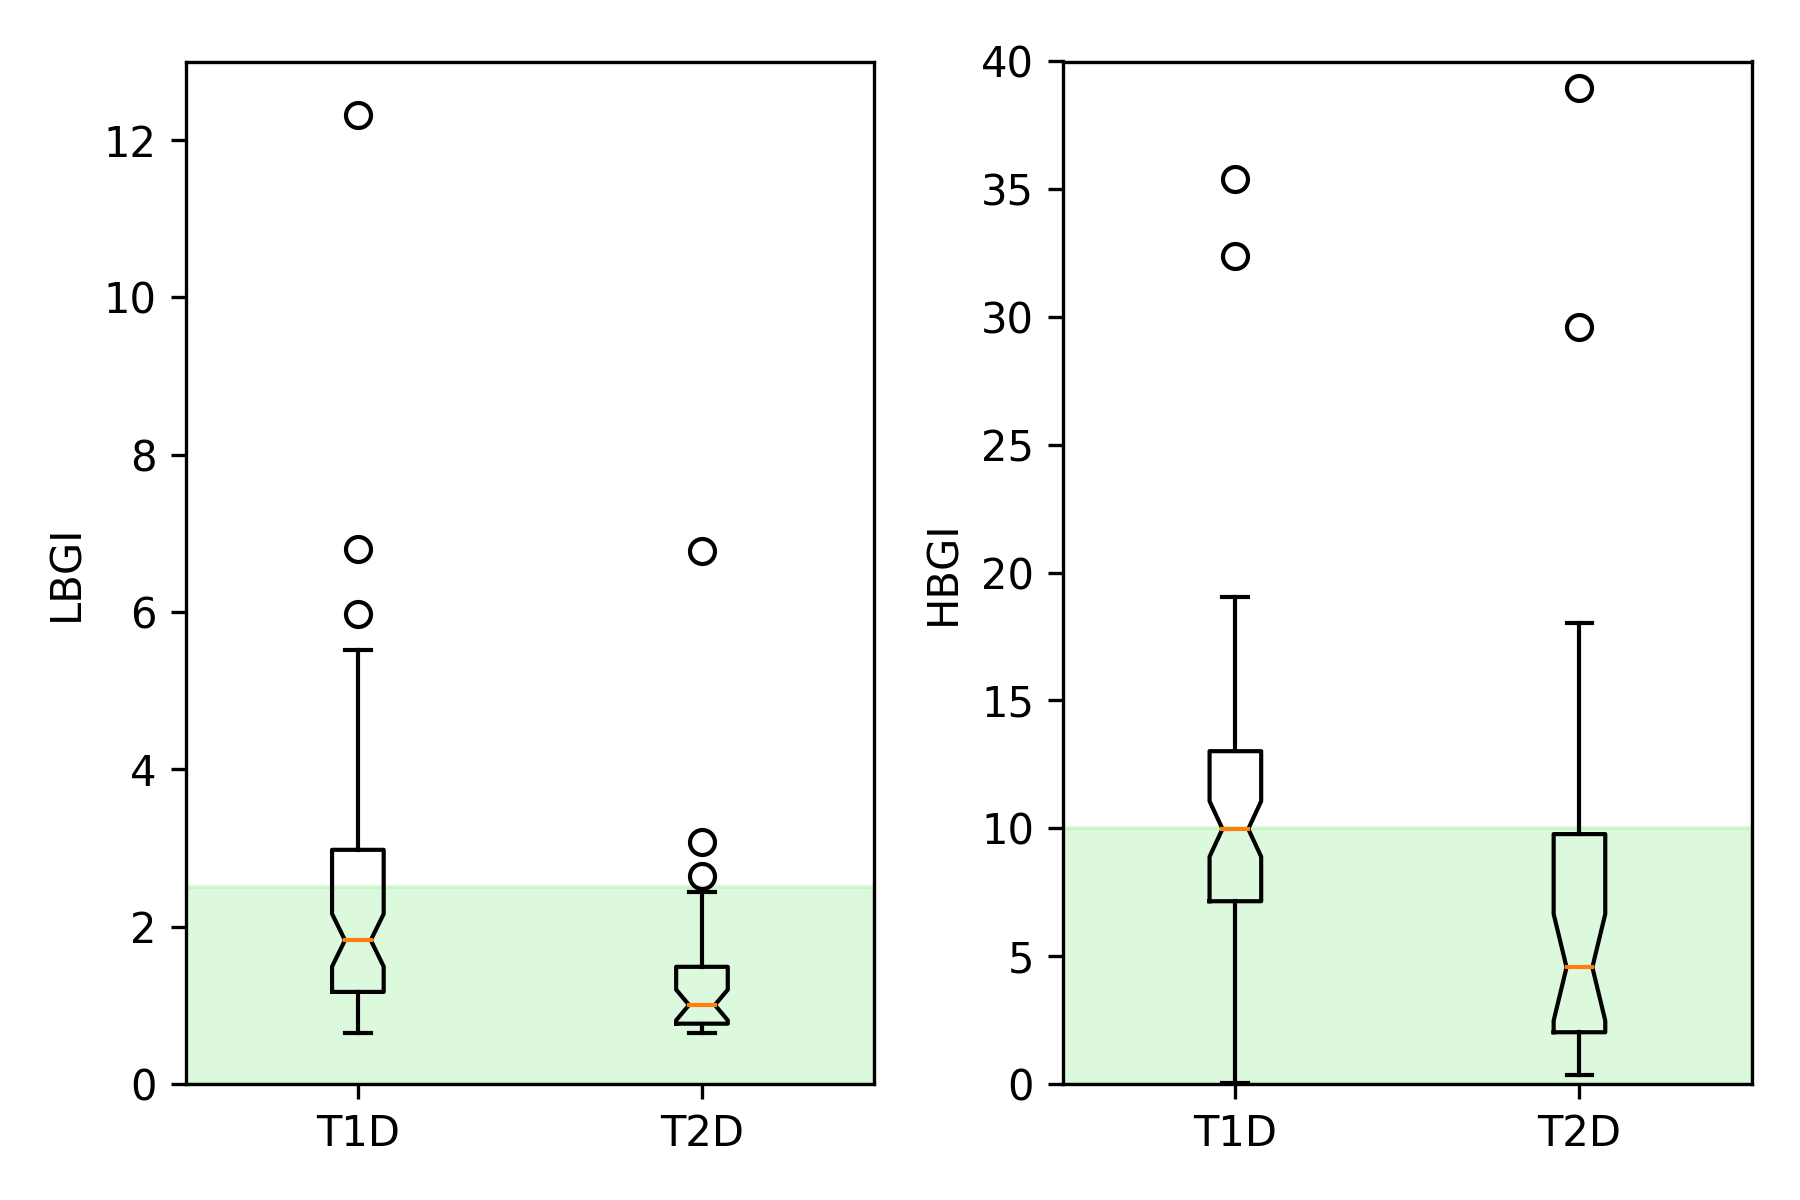
\includegraphics[width=0.8\textwidth]{part2/boxes.png}
\end{figure}

\section{CGM exploratory data analysis}
For each patient, the risk of hypo/hyperglycemia is determined by computing the Low Blood Glucose Index (\ac{LBGI}) and the High Blood Glucose Index (\ac{HBGI}), defined as in~\cite{fabris2016risk}.
LBGI and HBGI are summary statistics, extracted from a series of CGM data, that increases when the frequency and/or the extent of low CGM or high CGM readings increases.
These two indices are heavily influenced by the frequency and extent of hypo- and hyper-glycemic episodes.
To estimate LBGI and HBGI from CGM data we followed~\cite{kovatchev1997symmetrization}.
Figure \ref{fig:plots} shows the LBGI and HBGI distributions for T1D and T2D. The green areas at the bottom of each boxplot represents the low risk area for hypo/hyperglycaemia, as reported in literature~\cite{kovatchev1997symmetrization}.
As expected, the fraction of T1D patients experiencing risks of hyperglycaemia episodes is higher than T2D patients.


\begin{figure}
	\caption{An example of two glycemic profiles obtained from T1D and T2D patients. The glucose target range is set between $70$ mg/dL and $140$ mg/dL (dashed lines). The yellow area at the left hand side of the plot is the initial {\em burn-in} interval used for model {\em personalization}.}\label{fig:cgm}
	\centering
	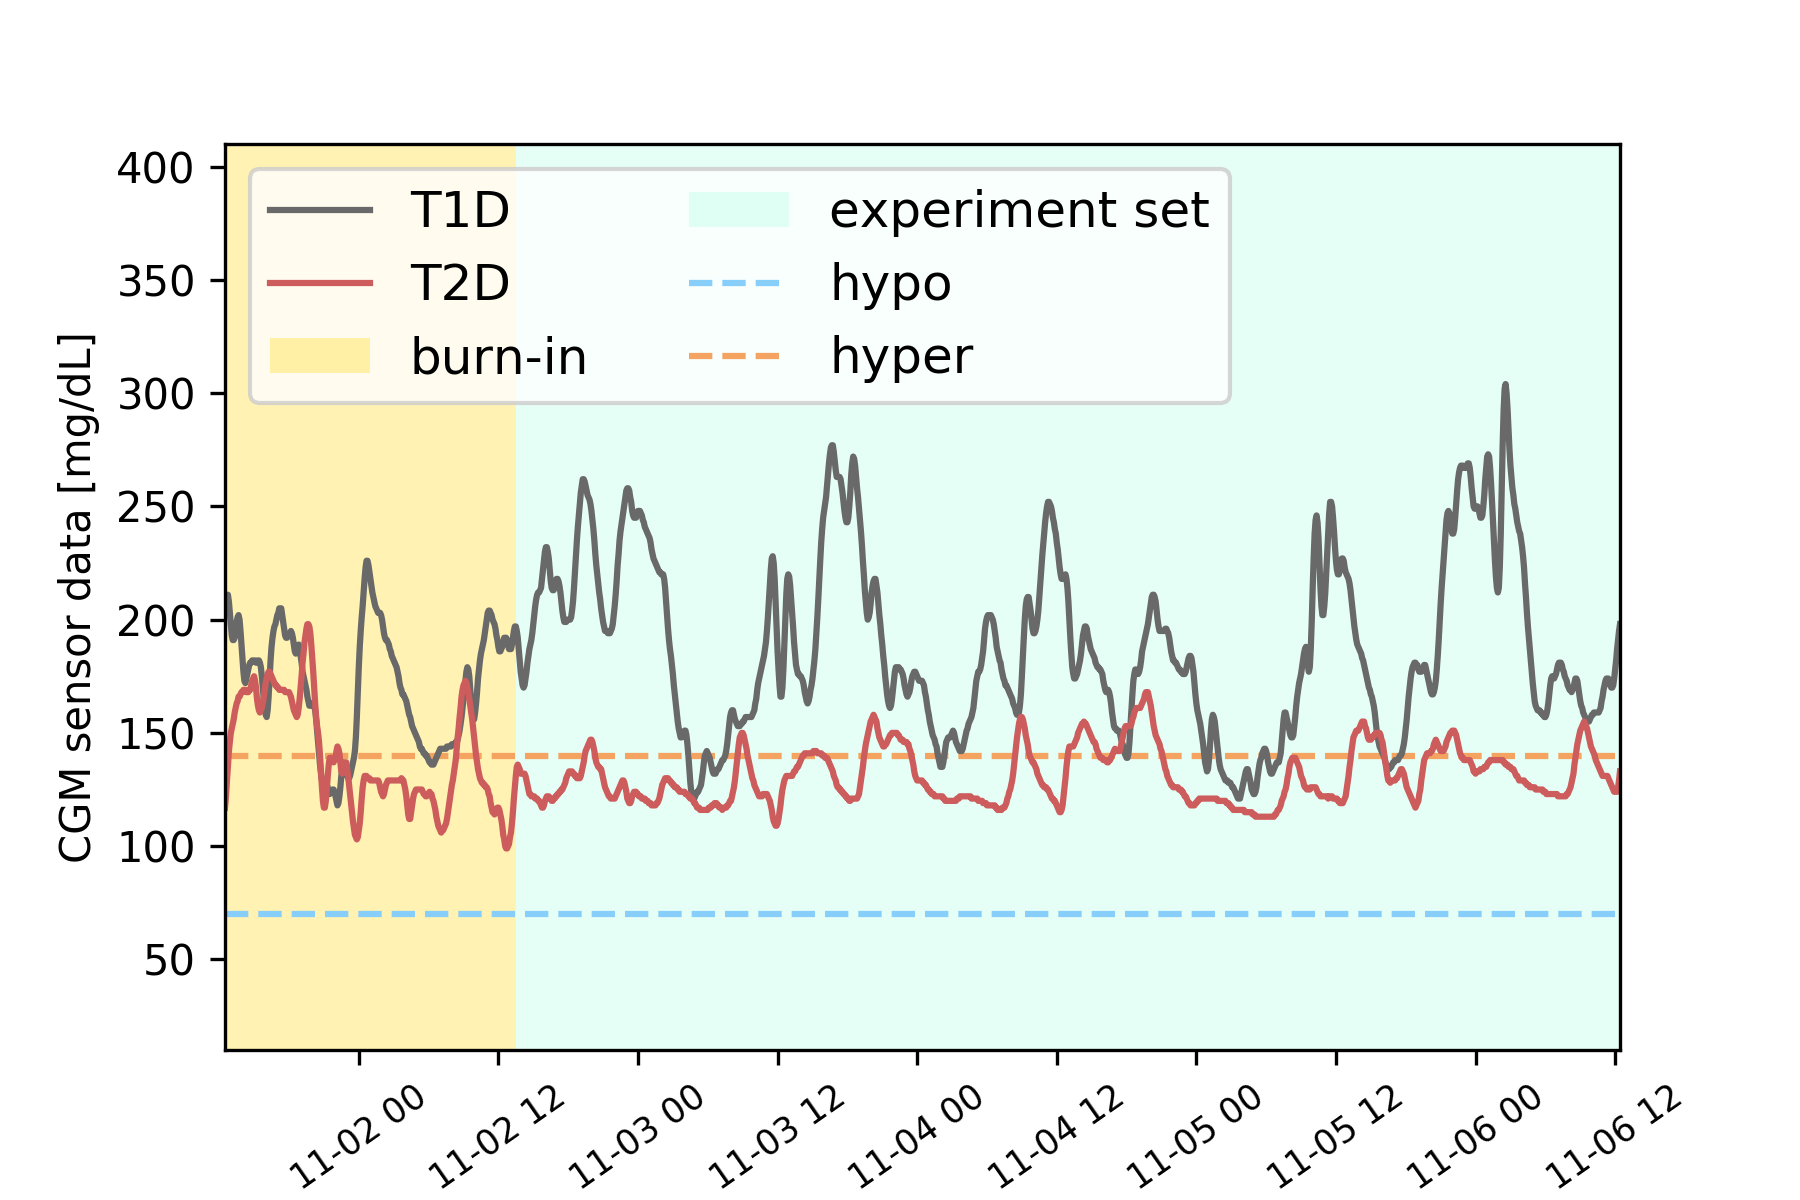
\includegraphics[width=0.8\textwidth]{part2/cgm_values.png}
\end{figure}

\section{Experimental design} \label{sec:diabete_expdesign}

We shall now focus on the hyperparameters optimization strategy.
Given $y(t)$ for time points $t=1,\dots,T$, we split the time-series in two chunks: an initial {\em burn-in} of $T' = 300$ CGM observations and the {\em experiment set} made of the subsequent $T - T'$ samples (see Figure~\ref{fig:cgm}). For each model $\mathcal{M}_\mathcal{S}(\bm{\theta})$, and for each subject, we use the burn-in samples to optimize the hyperparameters $\bm{\theta}$ via grid-search cross-validation. In other words, the best hyperparameters $\bm{\theta}^*$  are chosen as the ones that minimize an index $J(\bm{\theta})$ estimated on cross-validation splits and defined differently according to the model, as anticipated in the previous sections. %, hence $\bm{\theta}^* = \argmin{\bm{\theta}} J(\bm{\theta})$.

In the context of time-series, the cross-validation training splits consist only of observations occurred before the corresponding validation samples; such cross-validation flavor is sometimes referred to as {\em rolling forecasting origin}~\cite{tashman2000out}. The grid-search cross-validation scheme promotes the identification of models capable of returning robust predictions. %, where the negative influence of the variable SNR is reduced.

Once the best hyperparameters $\bm{\theta}^*$ are identified, the model $\mathcal{M}_\mathcal{S}(\bm{\theta}^*)$ is fitted on the whole burn-in and it is used to perform online forecasting on the data points of the experiment set (\ie for $t = T'+1, \dots, T)$.

For each personalized model $\mathcal{M}_\mathcal{S}(\bm{\theta}^*)$ we calculate the accuracy for prediction horizons $\Delta T$ of $30, 60, \text{and}~90$ minutes. The performance is estimated by  RMSE and MAE, defined in Section~\ref{sec:performance_metrics}, that in the context of temporal forecasting, and assuming $n$ samples in the experiment set, can be rewritten as in Equation~\eqref{eq:forecasting_rmse} and~\eqref{eq:forecasting_mae}.

\begin{equation} \label{eq:forecasting_rmse}
\text{RMSE} = \sqrt{\frac{\sum_t(y(t+\Delta T) - \hat{y}(t+\Delta T))^2}{n}}
\end{equation}

\begin{equation} \label{eq:forecasting_mae}
\text{MAE} = \frac{\sum_t|y(t+\Delta T) - \hat{y}(t+\Delta T)|}{n}
\end{equation}

%for $t = T'+1,\dots,T-\Delta T$.
%\todo{non abbiamo mai detto quando vale la window size (36) come in sparacino2007}
We use $w=36$ as the size of the window in the moving-window paradigm and we  indicate with $\{\bm{x}_i, y_i\}_{i=1}^N$  the input/output pairs for machine learning model. 
%Machine learning models need to be trained on input/output pairs $\{\bm{x}_i, y_i\}_{i=1}^N$. In this work we employed a moving-window paradigm of size $w=36$. 
Therefore, each input $\bm{x}_i$ is a $w$-dimensional vector made of the CGM samples acquired at times $t=t_{i-w},\dots,t_i$, while the corresponding output $y_i$ is the CGM acquisition at time $t_{i+1}$.


\section{CGM forecasting results}
Taking into account the available information on treatments, we divided the dataset into four groups, namely T1D with microinfusion pump (32 subjects), T1D with insulin injection (40 subjects), T2D with rapid acting insulin (10 subjects) and T2D with other therapies (24 subjects).

For each group, we applied all forecasting models whose performance, expressed in term of MAE and RMSE, is presented in Table~\ref{tab:errors}. 
%obtaining predictions similar to the example in Figure~\ref{fig:fit}.
%Results are reported in Table~\ref{tab:errors}.
%\todo{The dataset was divided into two groups The subjects were divided in four groups, according to their diabetes type and the followed therapy.}
%A summary of the forecasting performance of the four methods, 
The forecasting errors clearly increase with the prediction horizon as the errors accumulate at each predicted time step.

KRR achieves the most accurate prediction overall and for almost every group of patients, although ARIMA results are comparable. Moreover, KRR loss of reliability from the first to the last prediction horizon is lower than for ARIMA.

Figure~\ref{fig:fit} displays an example of time-series forecast obtained with KRR showing the three different prediction errors at $30$, $60$ and $90$ minutes.

%    Only the samples in the left side of the plot are assumed to be available (green line).

\begin{figure}[tb]
	\caption{Online time-series forecasting obtained by KRR model. \textit{One-step-ahead prediction} (left): the green solid line shows the available samples; the dashed line represents one-step-ahead predictions that are obtained by applying the model on a moving window of 36 time-points. \textit{Open-loop forecast} (right): with passing time, the moving-window incorporates an increasing number of predicted points, accumulating errors; the dashed line represents forecast with a prediction horizon of 90'.
	Absolute prediction errors are evaluated with respect to future measures (red solid line).
		%  The dashed line in the left side of the plot In the right side of the plot we simulate an open-loop forecast where 
		%  Assuming that only the samples in the left side of the plot are available, the figure shows one-step-ahead predictions.
		%  On the right side, forecasts for a prediction horizon of 90 minutes are shown. 
		%  The absolute errors reported are expressed in $mg/dL$.
	}\label{fig:fit}
	\centering
	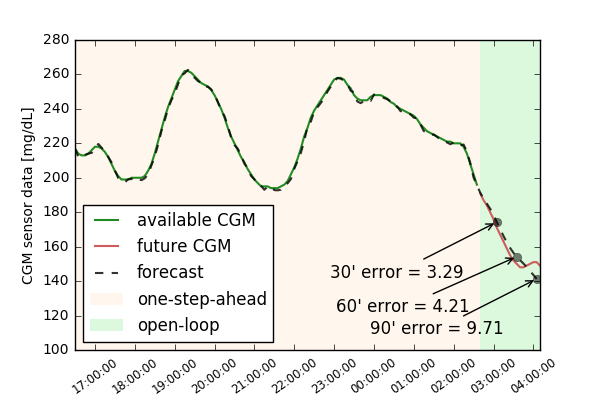
\includegraphics[width=0.8\textwidth]{part2/cgm_fit.png}
\end{figure}


\section{Conclusions and future works}

This chapter presented the last biomedical data science challenge of the thesis.

We compared the performance of two types of data-driven strategies for online CGM forecasting: recursive filters and ML models. We also illustrate a general procedure for model personalization based on cross-validation with hyperparameters optimization via grid-search.

Finally, we showed that reliable CGM predictions can be obtained with ML models that do not need to recursively adjust their parameters along time.
%In the next future we plan to investigate further using more advanced methods comprising deep learning approaches with  and sparse regularization methods.

In the future, to improve the performance on long prediction horizon, we plan to investigate sparse data representations with deeper architectures or regularized dictionary learning approaches.

\begin{table}[b!]
	\caption{Prediction errors (standard deviation) of the forecasting models for increasing prediction horizons, overall and on the four groups. {\sl MP} = Microinfusion Pump, {\sl II} = Insulin Injection, {\sl RAI} = Rapid Acting Insulin, {\sl Other} = Other therapies. Bold numbers indicate best result.}
	\label{tab:errors}
		\begin{tabular}{lllllll}
			& \multicolumn{6}{c}{ARIMA}                                              \\ \cline{2-7}
			\multicolumn{1}{l|}{}                           & \multicolumn{3}{c|}{MAE mg/dL}          & \multicolumn{3}{c|}{RMSE mg/dL}         \\ \cline{2-7}
			\multicolumn{1}{l|}{}                           & 30 & 60 & \multicolumn{1}{l|}{90} & 30 & 60 & \multicolumn{1}{l|}{90}  \\ \hline
			\multicolumn{1}{l|}{Overall}                    & 11.5 (5.2) & 25.6 (12.5) & \multicolumn{1}{l|}{37.2 (20.3)} & 16.7 (7.9) & 37.1 (19.3) & \multicolumn{1}{l|}{53.8 (31.8)} \\
			\multicolumn{1}{l|}{T1D - {\sl MP}}   & 13.3 (3.6) & 30.3 (7.4) & \multicolumn{1}{l|}{45.3 (12.5)} & 19.5 (5.4) & 43.9 (10.9) & \multicolumn{1}{l|}{64.9 (18.1)}  \\
			\multicolumn{1}{l|}{T1D - {\sl II}}    & 13.4 (6.3) & 31.0 (16.2) & \multicolumn{1}{l|}{46.1 (27.1)} & 19.7 (10.6) & 45.1 (27.0) & \multicolumn{1}{l|}{66.6 (45.7)}  \\
			\multicolumn{1}{l|}{T2D - {\sl RAI}} & {\bf11.0 (3.3)} & {\bf 23.8 (6.5)} & \multicolumn{1}{l|}{33.2 (8.5)} & 16.2 (4.8) & 34.1 (8.3) & \multicolumn{1}{l|}{46.9 (10.9)}  \\
			\multicolumn{1}{l|}{T2D - {\sl Other}}      & 10.0 (5.1) & 21.4 (10.4) & \multicolumn{1}{l|}{29.2 (12.5)} & 13.6 (6.0) & 29.6 (12.7) & \multicolumn{1}{l|}{41.3 (16.5)}  \\ \hline
			
			\\
			& \multicolumn{6}{c}{KF}                                                \\ \cline{2-7}
			\multicolumn{1}{l|}{}                           & \multicolumn{3}{c|}{MAE mg/dL}          & \multicolumn{3}{c|}{RMSE mg/dL}         \\ \cline{2-7}
			\multicolumn{1}{l|}{}                           & 30 & 60 & \multicolumn{1}{l|}{90} & 30 & 60 & \multicolumn{1}{l|}{90} \\ \hline
			\multicolumn{1}{l|}{Overall}              & 46.8 (23.2) & 50.8(25.4) & \multicolumn{1}{l|}{159.6 (43.5)} & 58.3 (27.7) & 63.1 (30.3) & \multicolumn{1}{l|}{169.9 (47.1)} \\
			\multicolumn{1}{l|}{T1D - {\sl MP}}         & 56.6 (15.9) & 59.5 (15.2) & \multicolumn{1}{l|}{163.5 (26.7)} & 70.5 (19.0) & 74.3 (18.4) & \multicolumn{1}{l|}{177.5 (29.9)} \\
			\multicolumn{1}{l|}{T1D - {\sl II}}    & 59.9 (24.5) & 67.9 (26.7) & \multicolumn{1}{l|}{179.2 (38.9)} & 74.4 (28.7) & 83.5 (31.3) & \multicolumn{1}{l|}{193.8 (40.4)} \\
			\multicolumn{1}{l|}{T2D - {\sl RAI}} & 48.6 (20.4) & 50.9 (20.8) & \multicolumn{1}{l|}{195.2 (63.1)} & 60.4 (22.9) & 63.6 (24.1) & \multicolumn{1}{l|}{204.4 (63.8)} \\
			\multicolumn{1}{l|}{T2D - {\sl Other}}      & 33.0 (12.1) & 35.6 (15.8) & \multicolumn{1}{l|}{145.0 (30.4)} & 41.3 (14.2) & 44.3 (17.7) & \multicolumn{1}{l|}{150.1 (31.8)} \\ \hline
			
			
			\\
			
			& \multicolumn{6}{c}{KRR}       \\ \cline{2-7}
			\multicolumn{1}{l|}{}                           & \multicolumn{3}{c|}{MAE mg/dL}          & \multicolumn{3}{c|}{RMSE mg/dL} \\ \cline{2-7}
			\multicolumn{1}{l|}{}                           & 30 & 60 & \multicolumn{1}{l|}{90} & 30 & 60 & \multicolumn{1}{l|}{90}  \\ \hline
			\multicolumn{1}{l|}{Overall}                    & {\bf 11.1 (4.3)} & {\bf 25.1 (10.4)} & \multicolumn{1}{l|}{{\bf 35.2 (15.4)}} & {\bf 15.5 (6.7)} & {\bf 33.6 (13.8)} & \multicolumn{1}{l|}{{\bf 45.8 (19.7)}} \\
			\multicolumn{1}{l|}{T1D - {\sl MP}}   & {\bf12.9 (3.4)} & {\bf 30.2 (8.4)} & \multicolumn{1}{l|}{{\bf 43.1 (12.6)}} & {\bf17.9 (5.1)} & {\bf 40.2 (10.9)} & \multicolumn{1}{l|}{{\bf 56.0 (16.1)}}  \\
			\multicolumn{1}{l|}{T1D - {\sl II}}    & {\bf13.1 (4.9)} & {\bf 30.3 (10.6)}  & \multicolumn{1}{l|}{{\bf 43.1 (14.5)}} & {\bf18.6 (8.4)} & {\bf 40.5 (14.5)} & \multicolumn{1}{l|}{{\bf 55.8 (18.6)}}  \\
			\multicolumn{1}{l|}{T2D - {\sl RAI}} & 11.2 (2.9) & 24.1 (5.5) & \multicolumn{1}{l|}{{\bf 33.2 (7.1)}} & {\bf16.0 (4.7)} & {\bf 32.7 (7.5)} & \multicolumn{1}{l|}{{\bf 43.7 (9.5)}}  \\
			\multicolumn{1}{l|}{T2D - {\sl Other}}      & {\bf8.7 (2.3)} & {\bf 19.8 (6.9)} & \multicolumn{1}{l|}{{\bf 27.7 (11.8)}} & {\bf11.9 (3.4)} & {\bf 26.5 (8.9)} & \multicolumn{1}{l|}{{\bf 36.2 (14.4)}}  \\ \hline
			
			\\
			
			& \multicolumn{6}{c}{LSTM}                                              \\ \cline{2-7}
			\multicolumn{1}{l|}{}                           & \multicolumn{3}{c|}{MAE mg/dL}          & \multicolumn{3}{c|}{RMSE mg/dL}         \\ \cline{2-7}
			\multicolumn{1}{l|}{}                           & 30 & 60 & \multicolumn{1}{l|}{90} & 30 & 60 & \multicolumn{1}{l|}{90} \\ \hline
			\multicolumn{1}{l|}{Overall}                & 19.9 (10.6) & 44.0 (25.9) & \multicolumn{1}{l|}{61.3 (36.5)} & 26.2 (13.4) & 55.0 (30.0) & \multicolumn{1}{l|}{74.7 (41.3)} \\
			\multicolumn{1}{l|}{T1D -{\sl  MP}}   & 22.9 (9.1) & 51.6 (21.5) & \multicolumn{1}{l|}{71.6 (27.0)} & 30.6 (11.6) & 65.7 (27.0) & \multicolumn{1}{l|}{89.8 (33.5)} \\
			\multicolumn{1}{l|}{T1D - {\sl II}}    & 24.5 (12.9) & 56.5 (33.1) & \multicolumn{1}{l|}{81.4 (45.8)} & 31.2 (14.9) & 68.8 (35.9) & \multicolumn{1}{l|}{97.0 (48.4)} \\
			\multicolumn{1}{l|}{T2D - {\sl RAI}} & 18.3 (6.7) & 39.4 (14.8) & \multicolumn{1}{l|}{54.1 (21.0)} & 25.7 (10.1) & 51.6 (21.7) & \multicolumn{1}{l|}{67.7 (29.1)} \\
			\multicolumn{1}{l|}{T2D - {\sl Other}}      & 16.8 (8.9) & 35.0 (17.7) & \multicolumn{1}{l|}{47.0 (26.5)} & 22.2 (12.1) & 43.4 (19.0) & \multicolumn{1}{l|}{56.5 (27.3)} \\ 
			
			\hline
			
		\end{tabular}
\end{table}



\part*{Part II}
\label{part:II}
\addcontentsline{toc}{part}{\nameref{part:II}} % REF NOT WORKING
% !TEX root = ../main.tex

%\cleardoublepage
\vspace*{\fill} 
\begin{displayquote}
	\begin{flushright}
	"\emph{Machine learning isn't mathematics or physics, where major advances can be done with a pen and a piece of paper. It's an engineering science.}"
	
	Fran\c{c}ois Chollet, Deep Learning with Python~\cite{chollet2018deep}
	\end{flushright}
\end{displayquote}
\cleardoublepage

% !TEX root = ../main.tex

\chapter{ADENINE: a Data exploration tool}
% ADENINE

% !TEX root = ../main.tex

\chapter{Model for metabolic age prediction} \label{chap:frassoni}
% Frassoni sani + CCS

%Per rispondere alla richiesta di Samuele:
%- MDA (malondialdeide) è un marcatore della perossidazione lipidica, quindi dello stress ossidativo
%- Consumo d'ossigeno e ATP sintesi con P/M: valutazione del consumo di ossigeno e sintesi di ATP in presenza di piruvato e malato che stimolano la via mitocondriale composta da Complesso I, III e IV (valuta la funzionalità del mitocondrio)
%- Consumo d'ossigeno e ATP sintesi con succinato: valutazione del consumo di ossigeno e sintesi di ATP in presenza di succinato che stimola la via mitocondriale composta da Complesso II, III e IV (valuta la funzionalità del mitocondrio)
%- ATP: concentrazione intracellulare di ATP
%- AMP: concentrazione intracellulare di AMP
%- ATP/AMP: rapporto tra le due precedenti  misure che indica lo stato energetico cellulare ( più elevato più la cellula possiede energia)
%- LDH: attività della lattico deidrogenasi, ultimo enzima del pathway della glicolisi anaerobia (antagonista della fosforilazione ossidativa che noi valutiamo tramite i consumo d'ossigeno e la sintesi di ATP).

\begin{displayquote}
	\textit{In this chapter, we evaluate the changes of energy metabolism during the physiological aging. To this aim we will develop a ML model that predicts the age of an individual starting from the following molecular biomarkers: oxidative phosphorylation efficiency, the \ac{ATP}/\ac{AMP} ratio, the lactate dehydrogenase activity and the level of malondialdehyde.  For this purpose we employed mononuclear cells obtained from healthy population with age between $5$ and $106$ years.}
\end{displayquote}

\section{Introduction: aging and metabolism} \label{sec:frassoni_intro}

In this chapter we present the first biomedical data science problem of the thesis. The problem consists in analyzing a set of molecular biomarkers collected from $118$ volunteers with the final aim of devising a ML model capable of predicting the age of an individual\footnote{this was referred to as \textit{the aging problem} throughout Chapter~\ref{chap:state-of-the-art}}. In order to achieve such model, extensive EDA  and thorough model selection will be performed.
Before diving into the experimental setup, let's see some preliminary biological notions of how aging influences our metabolism.

Aging is a multifactorial process characterized by a progressive decline of physiological functions~\cite{campisi2013aging}, which leads to an increment of vulnerability and the relative risk of disease and death ~\cite{bratic2010mitochondrial}.

Aging represents the primary risk factor for several chronic pathologies, \ie cancer, cardiovascular disorders, diabetes and neurodegeneration~\cite{lopez2013hallmarks}. Different molecular pathways seem involved in the aging process, including deregulated autophagy, mitochondrial dysfunction, telomere shortening, oxidative stress, systemic inflammation, and metabolism dysfunction~\cite{lopez2013hallmarks, riera2016signaling}.

Recently, an involvement of epigenetic modifications has been proposed~\cite{thompson2017epigenetic}, developing an \textit{aging clock} based on the degree of DNA methylation, which increases with the age~\cite{horvath2013dna}. However, for several years, aging has been considered the result of damages accumulation due to an excessive production of reactive oxygen species (ROS).

The \textit{Mitochondrial Theory of Aging}~\cite{harman1972biologic, sastre2000mitochondrial} derives from the  concept that mitochondria are the main source of oxidative stress~\cite{cadenas2000mitochondrial, turrens2003mitochondrial, dai2014mitochondrial} and the fact that mitochondrial DNA displays a
great rate of mutation together with a less efficient repair machinery with respect to nuclear DNA~\cite{short2005decline}. After some mitochondrial DNA mutation threshold, irreversible oxidative damages propagate throughout the genome. This phenomenon leads to dysfunction of mitochondrial metabolism~\cite{genova2004mitochondrial} accelerating the oxidative stress production~\cite{wallace2010mitochondrial}.

As shown in~\cite{mckerrell2015leukemia}, mononuclear cells isolated from peripheral blood, are an excellent model to evaluate the metabolic status of an entire organism. In fact, the molecular alterations identified in peripheral blood cells of aged normal subjects are statistically correlated with degenerative diseases~\cite{jaiswal2014age}.

%Moreover, we have trained on the collected data a machine learning model that aims at predicting the age of an individual based on its metabolic markers (features). Thanks to the adopted shrinkage penalties, the obtained model is at the same time robust to the noise in the data and capable of exploiting the collinearity among the features \cite{hastie2009elements}. The statistical soundness of the obtained model is thoroughly tested by extensive data resampling and refitting strategies \cite{molinaro2005prediction}. The achieved model attains an expected error of XXX years.

\section{Data collection} \label{sec:frassoni_data_collection}

The study presented in this chapter is performed on mononuclear cells isolated from peripheral blood obtained from a population of $118$ volunteers\footnote{all participants provided their written informed consent to participate in this study, which was approved by the Ethics Committee of the IRCCS Istituto G. Gaslini, Genoa, IT, \todo{(N°)}} with age between $8$ and $106$ years.
In order to preserve the collected blood samples, the vacutainer tubes were transferred into the laboratory and analyzed within $24$ hours from collection.
All chemicals were purchased from Sigma Aldrich (St. Louis, MO, USA), unless otherwise indicated. Ultrapure water (Milli-Q; Millipore, Billerica, MA, USA) was used throughout. All other reagents were of analytical grade.
Data collection and further analysis were managed by a team of specialized biologists at the IRCCS Istituto G. Gaslini, Genoa, IT. On each blood sample, we performed the following measures.

\begin{itemize}
	\item[] \textbf{ATP} This complex molecule is the main responsible for storing and exchanging energy in cells and it is often referred to as the \textit{energy currency} of the cell. From a chemical point of view, ATP is made of an adenine base attached to a ribose sugar, which, in turn, is attached to three phosphate groups.
	ATP is heavily involved in different cellular aerobic respiration pathways. High levels of ATP correspond to high energetic state.
	ATP intracellular concentration, measured in $\text{mM}/\text{ml}$, is an important molecular biomarker to evaluate the energetic state of a cell.
	
	\item[] \textbf{AMP} This molecule is one of the main derivatives of ATP. In fact, AMP ca be obtained when two phosphate groups are removed from ATP, releasing energy that can be transferred to other molecules to trigger some further cell reaction.
	Therefore, when a cell is in good health, \ie high energetic level, AMP is low (and ATP is high).
	AMP cellular concentration is measured in $\text{mM}/\text{ml}$ and it is considered as an important molecular biomarker for the cellular energetic state. ATP and AMP quantification was based on the enzyme coupling method presented in~\cite{ravera2013tricarboxylic}.
%	as a side product of the ATP synthesis process or 
	
	\item[] \textbf{ATP/AMP ratio} With the aim of predicting the age of an individual by assessing the energetic state of the peripheral blood cells, measuring ATP and AMP cellular concentration may not be enough. A more representative and interesting quantity can be their ratio, so ATP/AMP ratio was calculated and added to the feature set.
	
	\item[] \textbf{Oxygen consumption} Aerobic cellular respiration requires oxygen to produce ATP. Therefore, the cellular oximetric level is an important molecular biomarker for the cellular metabolic assessment. Oxygen consumption was measured with an amperometric electrode in a closed chamber, magnetically stirred, at 37°C. The oxygen consumption measure, expressed in $\text{nmol~O}_2/(\text{min}\cdot\text{mg})$, is repeated in two versions, adding two different substrates, \ie
	\begin{enumerate*}[label=(\roman*)]
		\item a combination of $5~\text{mM}$ pyruvate with $2.5~\text{mM}$ malate or
		\item only $20~\text{mM}$ succinate.
	\end{enumerate*}
	In the first oximetric measure, which from now on will be referred to as \copyrmal, the substrate stimulates the pathway composed by Complexes I, III and IV. On the other hand, in the second oximetric measure, which we call \cosucc, the substrate activates the pathway composed by Complexes II, III and IV, as described in~\cite{cappelli2017defects}.
	
	\item[] \textbf{ATP synthesis} We already covered the importance of the ATP for the evaluation of the metabolic state of cells. We also measured ATP synthesis, expressed in $\text{nmol~ATP}/(\text{min}\cdot\text{mg})$,  by the highly sensitive luciferin/luciferase method. The same two substrates used for the oximetric evaluation were adopted. In the remainder of the chapter we refer to such measures as \atppyrmal and \atpsucc, accordingly.
	
	\item[] \textbf{P/O ratio} In order to assess the efficiency of oxidative phosphorylation, we also evaluated the ratio between ATP synthesis and oxygen consumption under both the substrates. We call the two obtained features as \popyrmal and \posucc, respectively.
	
	\item[] \textbf{Glycolytic flux} In order to assay the glycolytic flux, we measured the activity of the Lactate Dehydrogenase (\ac{LDH}), expressed in $\text{U}/\text{mg}$. This enzyme is important to evaluate the other metabolic pathway not mentioned so far, \ie the anaerobic respiration.
	
	\item[] \textbf{Lipid peroxidation} The uncoupled oxidative phosphorylation metabolism is often associated with an increment in the oxidative stress production~\cite{dai2014mitochondrial}, which induces damages on proteins, nucleic acid and membrane. Therefore, we evaluated the level of malondialdehyde (\ac{MDA}) as a marker of lipid peroxidation. The measure of \mda follows the protocol in~\cite{ravera2015oxidative}.	
\end{itemize}

Each sample of this dataset is then described by the $12$-dimensional feature set summarized in Table~\ref{tab:aging_features}.

\begin{table}[]
	\centering
	\caption{The $12$-dimensional feature set.}
	\label{tab:aging_features}
	\begin{tabular}{@{}ll@{}}
		\toprule
		\textbf{Measure}                                    & \textbf{Feature name}\\ \midrule
		Gender of the individual                      & sex          \\
		ATP intracellular concentration            & \atp         \\
		AMP intracellular concentration            & \amp         \\
		ATP/AMP ratio                              & \atpamp      \\
		Oxygen consumption under Pyruvate + Malate & \copyrmal    \\
		Oxygen consumption under Succinate         & \cosucc      \\
		ATP synthesis under Pyruvate + Malate      & \atppyrmal   \\
		ATP synthesis under Succinate              & \atpsucc     \\
		P/O ratio under Pyruvate + Malate          & \popyrmal    \\
		P/O ratio under Succinate                  & \posucc      \\
		Glycolytic flux                            & \ldh         \\
		Lipid peroxidation                         & \mda         \\ \bottomrule
	\end{tabular}
\end{table}


\section{Exploratory data analysis} \label{sec:frassoni_EDA}
% BOXPLOT - PCA - HEATMAP etc
In this section we investigate on the relationship between the collected molecular biomarker and the age of the 118 healthy individuals involved in this study.

The data collection process entirely ran on voluntary basis. So, it is interesting to investigate on the resulting age distribution. As we can see from the histogram in Figure~\ref{fig:frassoni_agehist}, not each decade is equally represented. Ideally, we would have collected samples with uniformly distributed, but this was unfortunately not possible. Therefore, we shall provide appropriate countermeasures to avoid bias in the following supervised regression step.

\begin{figure}[]
	\centering
	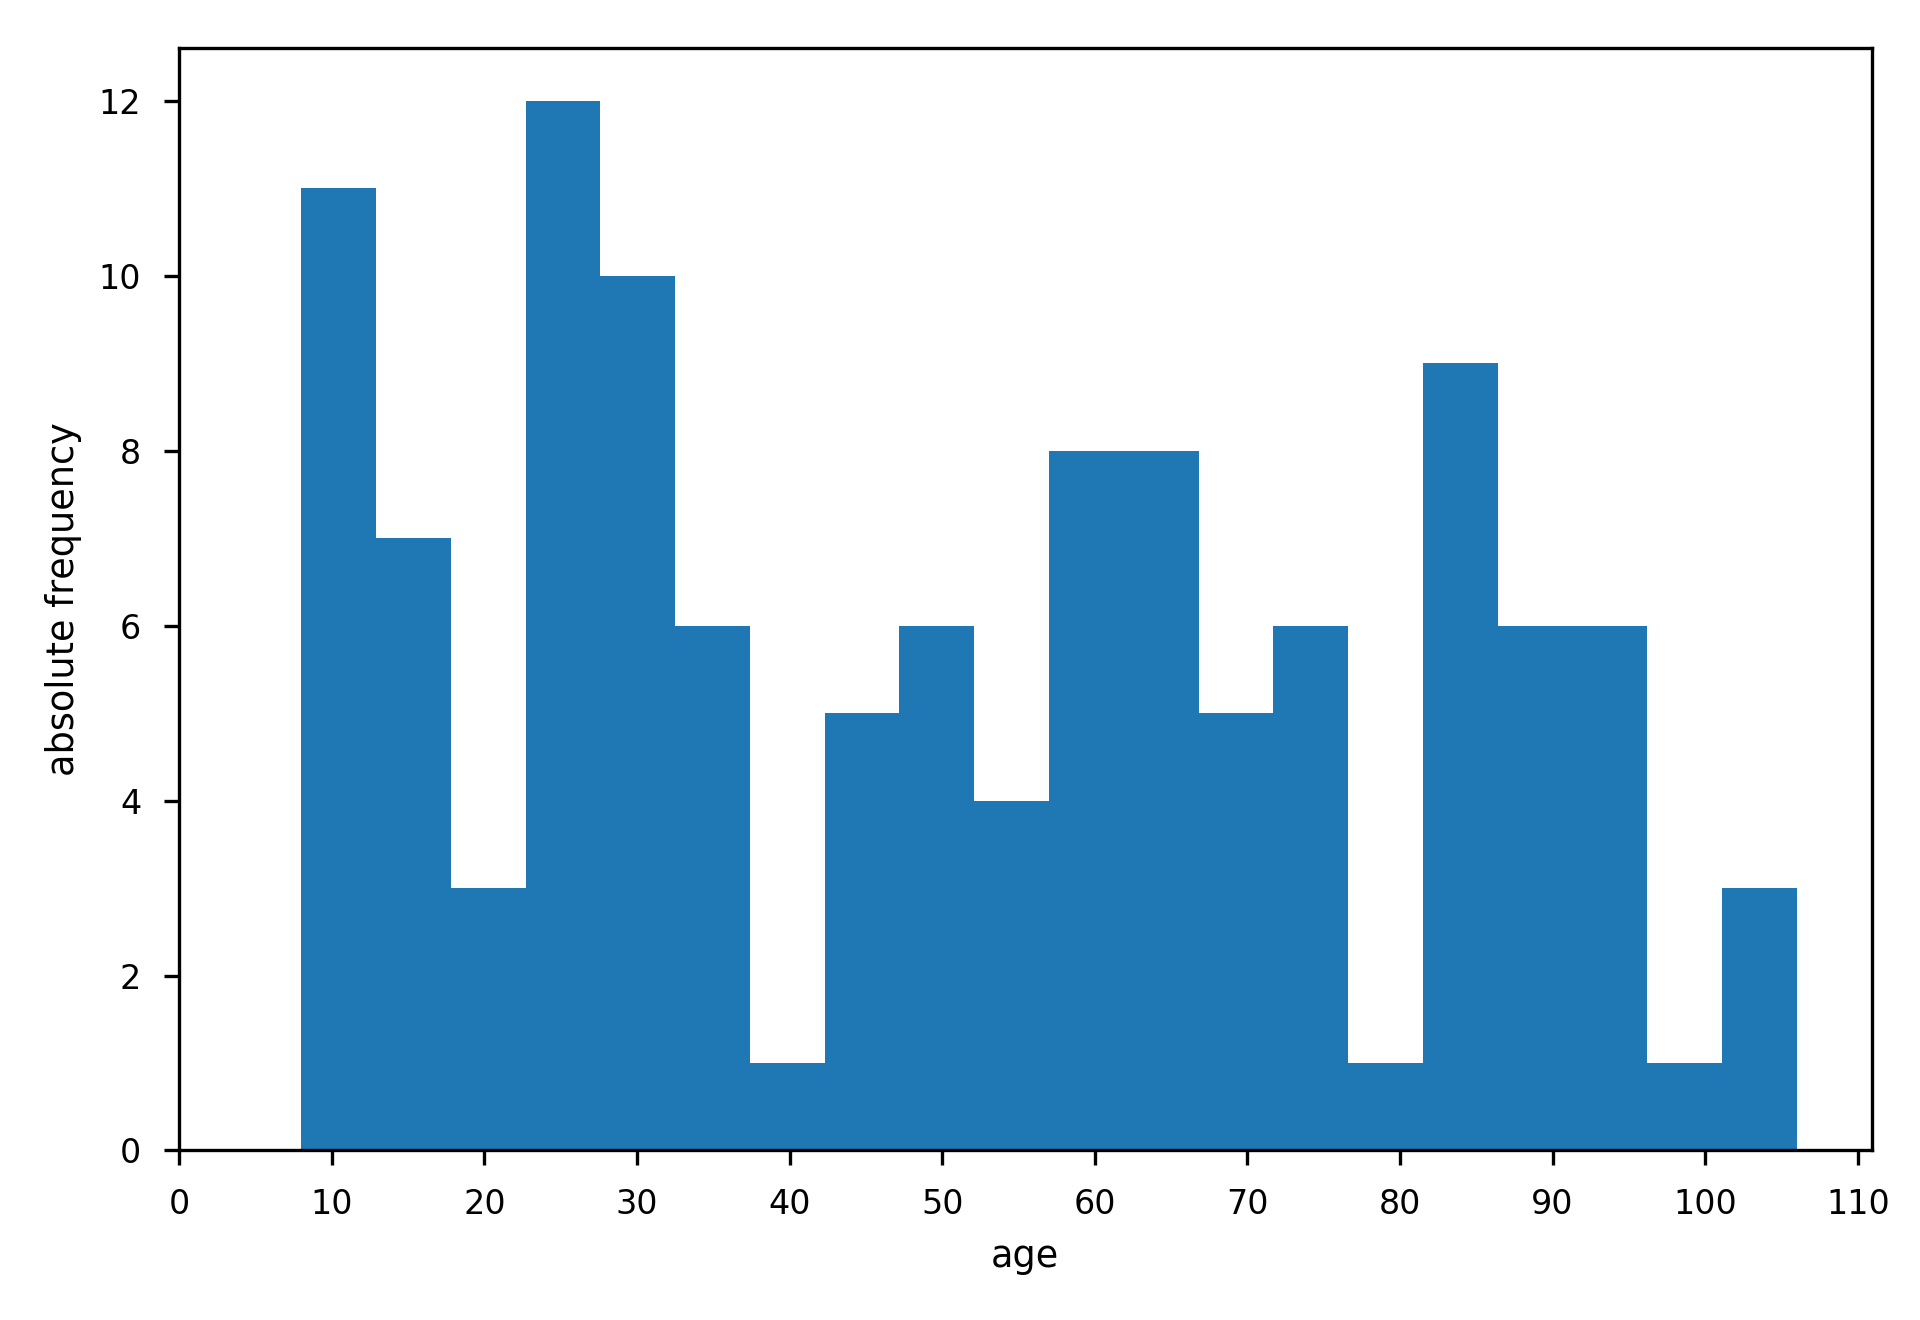
\includegraphics[width=0.8\textwidth]{part2/aging_agehist.png}
	\caption{Age distribution of the $118$ individuals involved in the study.} \label{fig:frassoni_agehist}
\end{figure}

Next, we aim at investigating on how the distribution of the molecular biomarker is influenced by the age of the individuals. To this aim we group the measures per decade and we represent the distribution with boxplots, see Figure~\ref{fig:frassoni_boxplot}.
As we can see, most of the biomarkers show a clear trend with the age. In particular, focusing our attention on the \atpamp ratio ($3^{\text{rd}}$ row, $3^{\text{rd}}$ column of Figure~\ref{fig:frassoni_boxplot}), which is known to be an energy status monitor of the cells, we can see that the values decrease progressively with the decades, with a drastic decrease between $40$ and $50$ years. Moreover, from an observation of \atp and \amp intracellular concentration ($3^{\text{rd}}$ row, $1^\text{st}$ and $2^\text{nd}$ column, respectively) we can sense how the increase of their ratio is mainly due to the grow of \amp in the aging process.


\begin{figure}[]
	\centering
	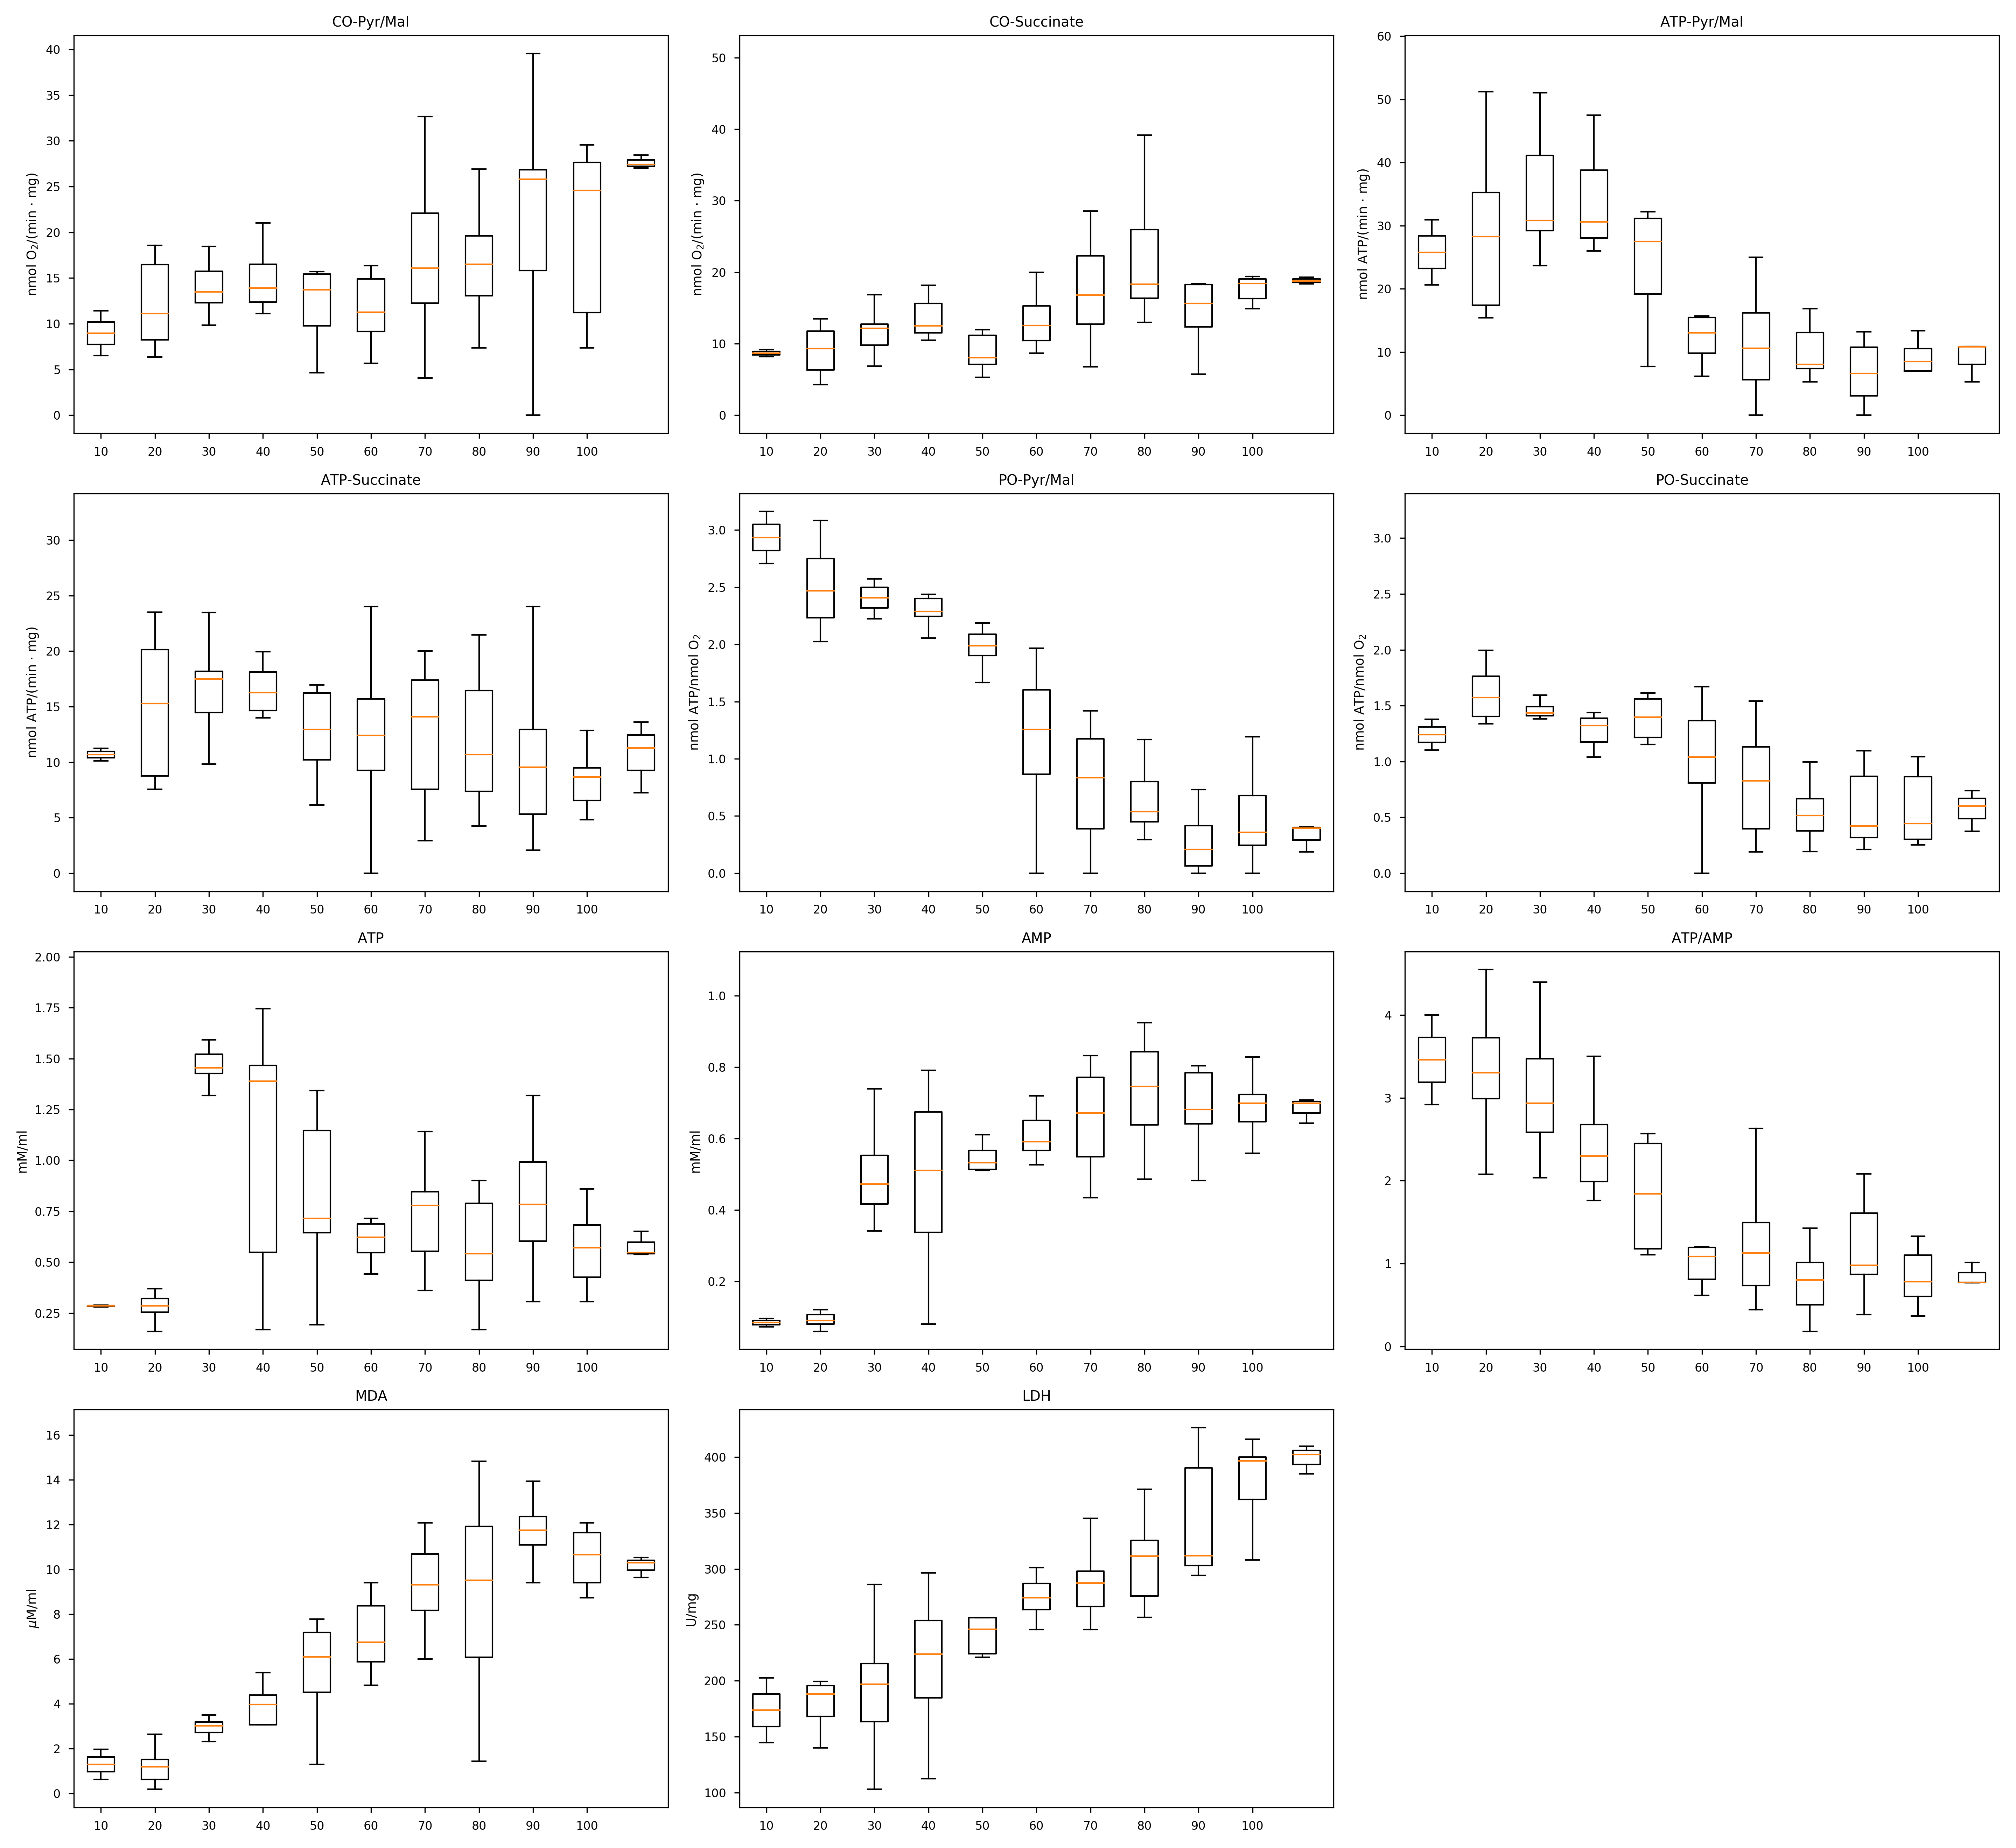
\includegraphics[width=0.8\textwidth]{part2/aging_boxplot.png}
	\caption{Distribution of the collected biomarkers grouped per decade.} \label{fig:frassoni_boxplot}
\end{figure}


\section{Metabolic age prediction} \label{sec:frassoni_regression}
% pipeline + assessment + model challenge

\section{Results} \label{sec:frassoni_results}
% tabella dei risultati

\section{Conclusions and future works} \label{sec:frassoni_conclusions}
% CCS

future: collect more data in order to have a uniformly distributed dataset

%%
% !TEX root = ../main.tex

\chapter{Temporal prediction of multiple sclerosis evolution from patient-centered outcomes} \label{chap:aism}
% AISM

\begin{displayquote}
%	This chapter describes a patient-centered outcomes-based ML model that predicts the disease evolution of multiple sclerosis patients.
	In this chapter, we investigate on
	use of patient-centered outcomes to predict the evolution of multiple sclerosis and to assess its impact on patients' lives.
	Multiple Sclerosis is a degenerative condition of the central nervous system that affects nearly $2.5$ million of individuals in terms of their physical, cognitive, psychological and social capabilities. Despite the high variability of its clinical presentation, \textit{relapsing} and \textit{progressive} multiple sclerosis are considered the two main disease types, with the former possibly evolving into the latter.
	%Nowadays no acknowledged clinical tests to diagnose multiple sclerosis or to distinguish between its types have been proposed.
	Recently, the attention of the medical community toward the use of patient-centered outcomes in multiple sclerosis has significantly increased. Such patient-friendly measures are devoted to the assessment of the impact of the disease on several domains of the patient life.
	% One of the open questions in the field is the use of patient-centered outcomes to assess multiple sclerosis impact on patients' lives and to predict the evolution of the disease.
	%To date, a clear understanding on whether it is possible to define a predictive model based on them is still an open question.
	%the use of such measures to assess neurodegenerative diseases evolution is still lacking. Moreover,
	To this aim, we build a novel temporal model based on gradient boosting classification and multiple-output elastic-net regression. The model
	%  is entirely based on patient-centered outcomes and it
	provides clinically interpretable results along with accurate predictions of the disease course evolution.
\end{displayquote}

\section{Introduction: the evolution of multiple sclerosis} \label{sec:aism_intro}

Multiple Sclerosis (MS) is a neurodegenerative and chronic disease of the central nervous system characterized by damages to the myelin sheaths, resulting in a wide range of symptoms, such as fatigue, numbness, visual disturbances, bladder problems, mobility issues and cognitive deficits.

% \todo{In clinical practice, accurate patient evaluation and clinical judgement remain the basics in MS diagnosis, as the identification of a validated set of biomarkers is still an open problem~\cite{milo2014revised}.}

People with MS (PwMS) are mainly classified according to their disease course:
relapsing-remitting (\ac{RR}), secondary-progressive (\ac{SP}), primary-progressive (\ac{PP}) and progressive-relapsing (\ac{PR})~\cite{giovannoni2016brain} and benign (\ac{B}).
Neurological disability in \RR patients is mainly due to the development of multifocal inflammatory lesions and it results in relapses, that are attacks of neurological worsening (\ie \textit{relapses}), followed by partial or complete recovery. Disability accrues predominantly in progressive courses (\SP, \PP, \PR) that are more characterized from diffuse immune mechanisms and neurodegeneration.
Benign MS occurs when the patient remains fully functional in all neurologic systems for at least $15$ years after the onset.
Figure~\ref{fig:ms_mock} shows a representative disability progression of MS patients according to their disease course.

An estimated $15\%$ of PwMS have a \PP or \PR course at the onset, the remaining $85\%$ is diagnosed with a \RR course.
About $80\%$ of \RR patients develop \SP course within $15\text{--}20$ years if untreated, or if the adopted pharmacological and rehabilitative protocols are not continuously adjusted according to the evolution of the disease~\cite{scalfari2014onset}.

\begin{figure}[]
	\centering
	\subfloat[]{%
		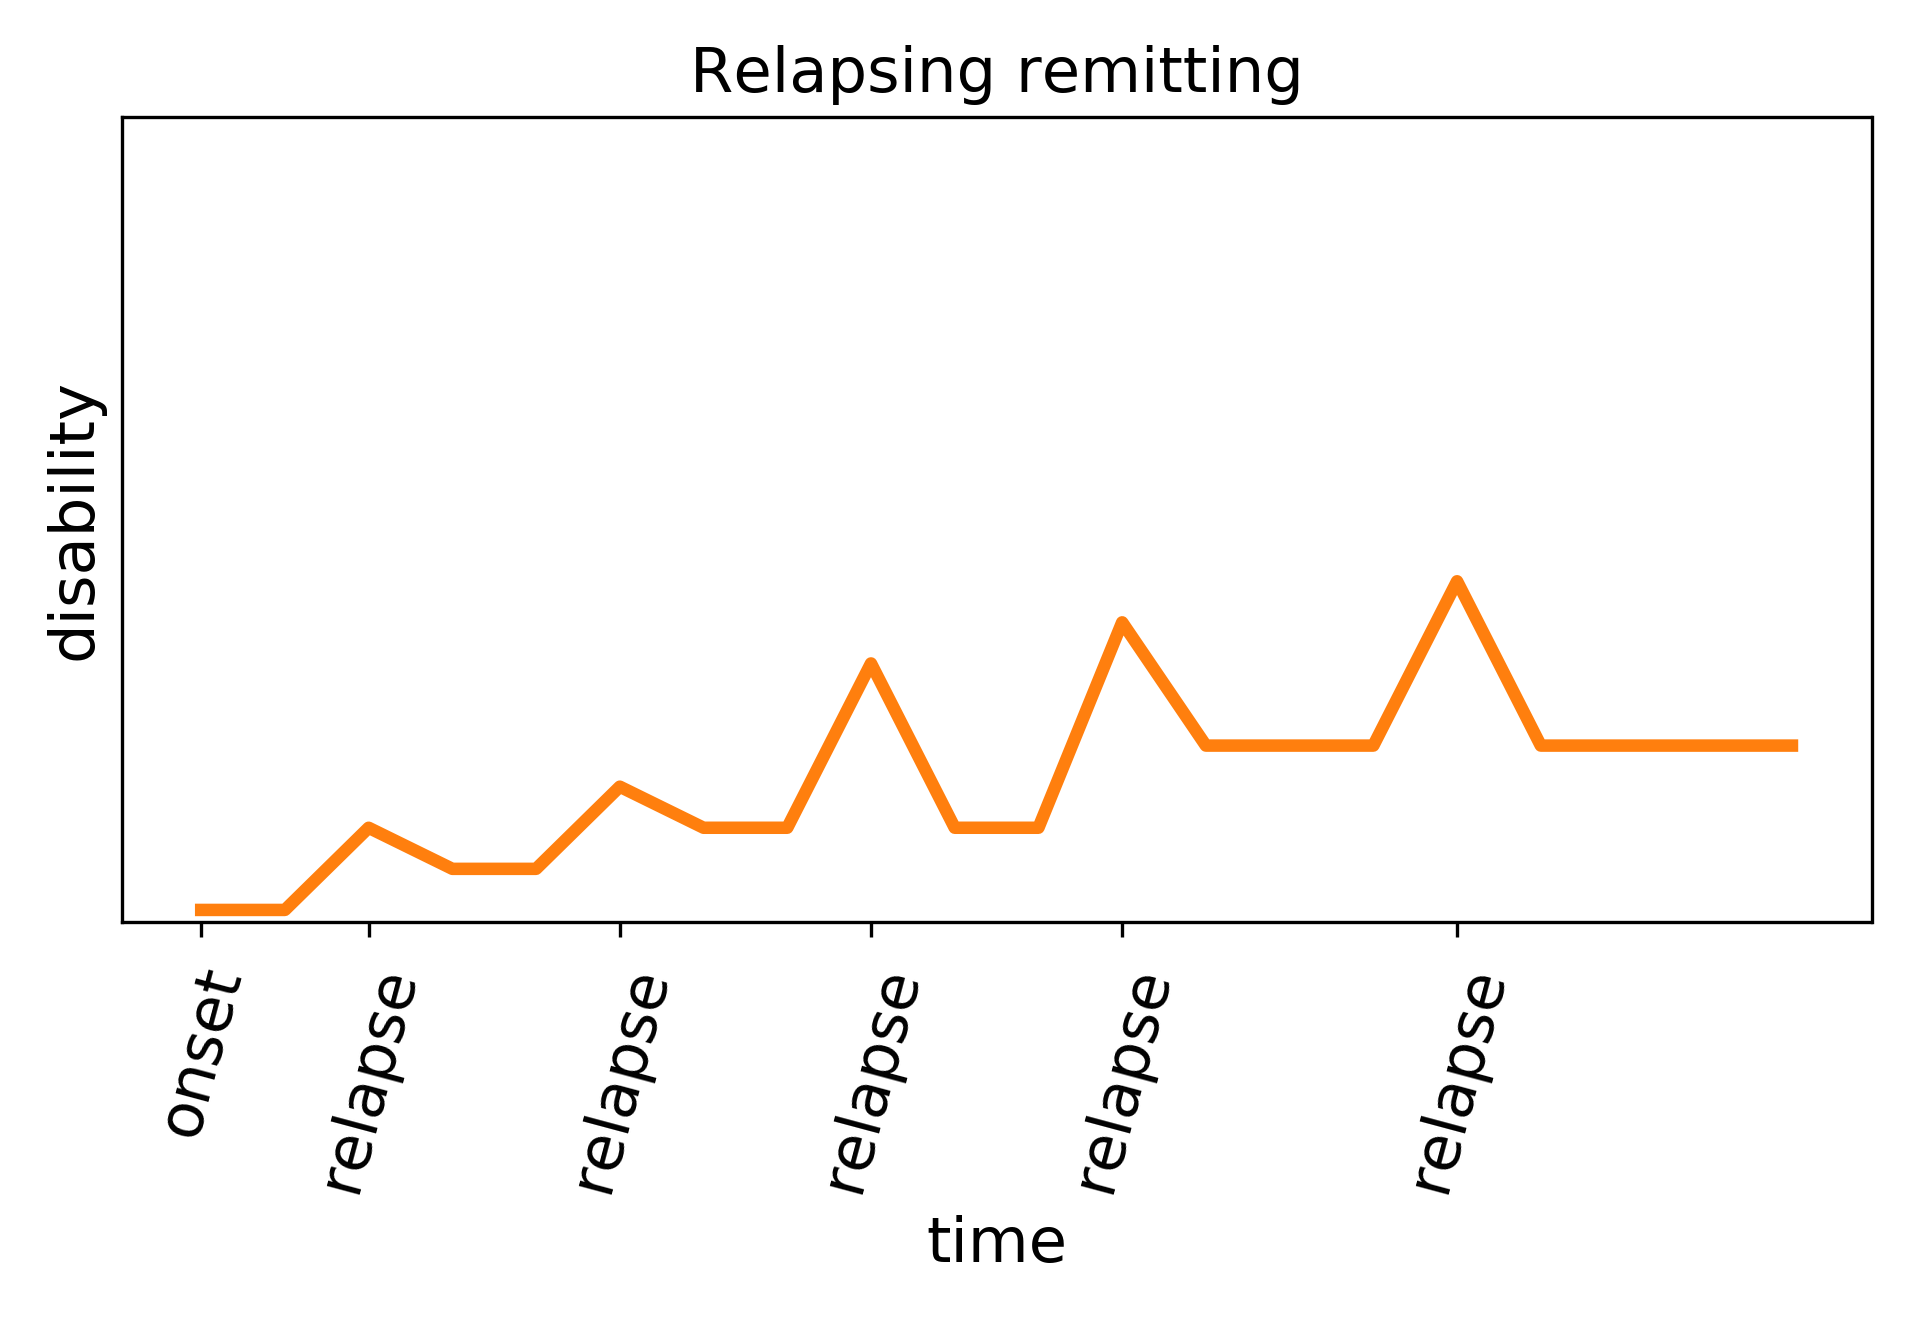
\includegraphics[width=0.5\textwidth]{part2/ms_mock_rr.png}
		\label{fig:ms_mock_rr}%
	}%
	\subfloat[]{%
		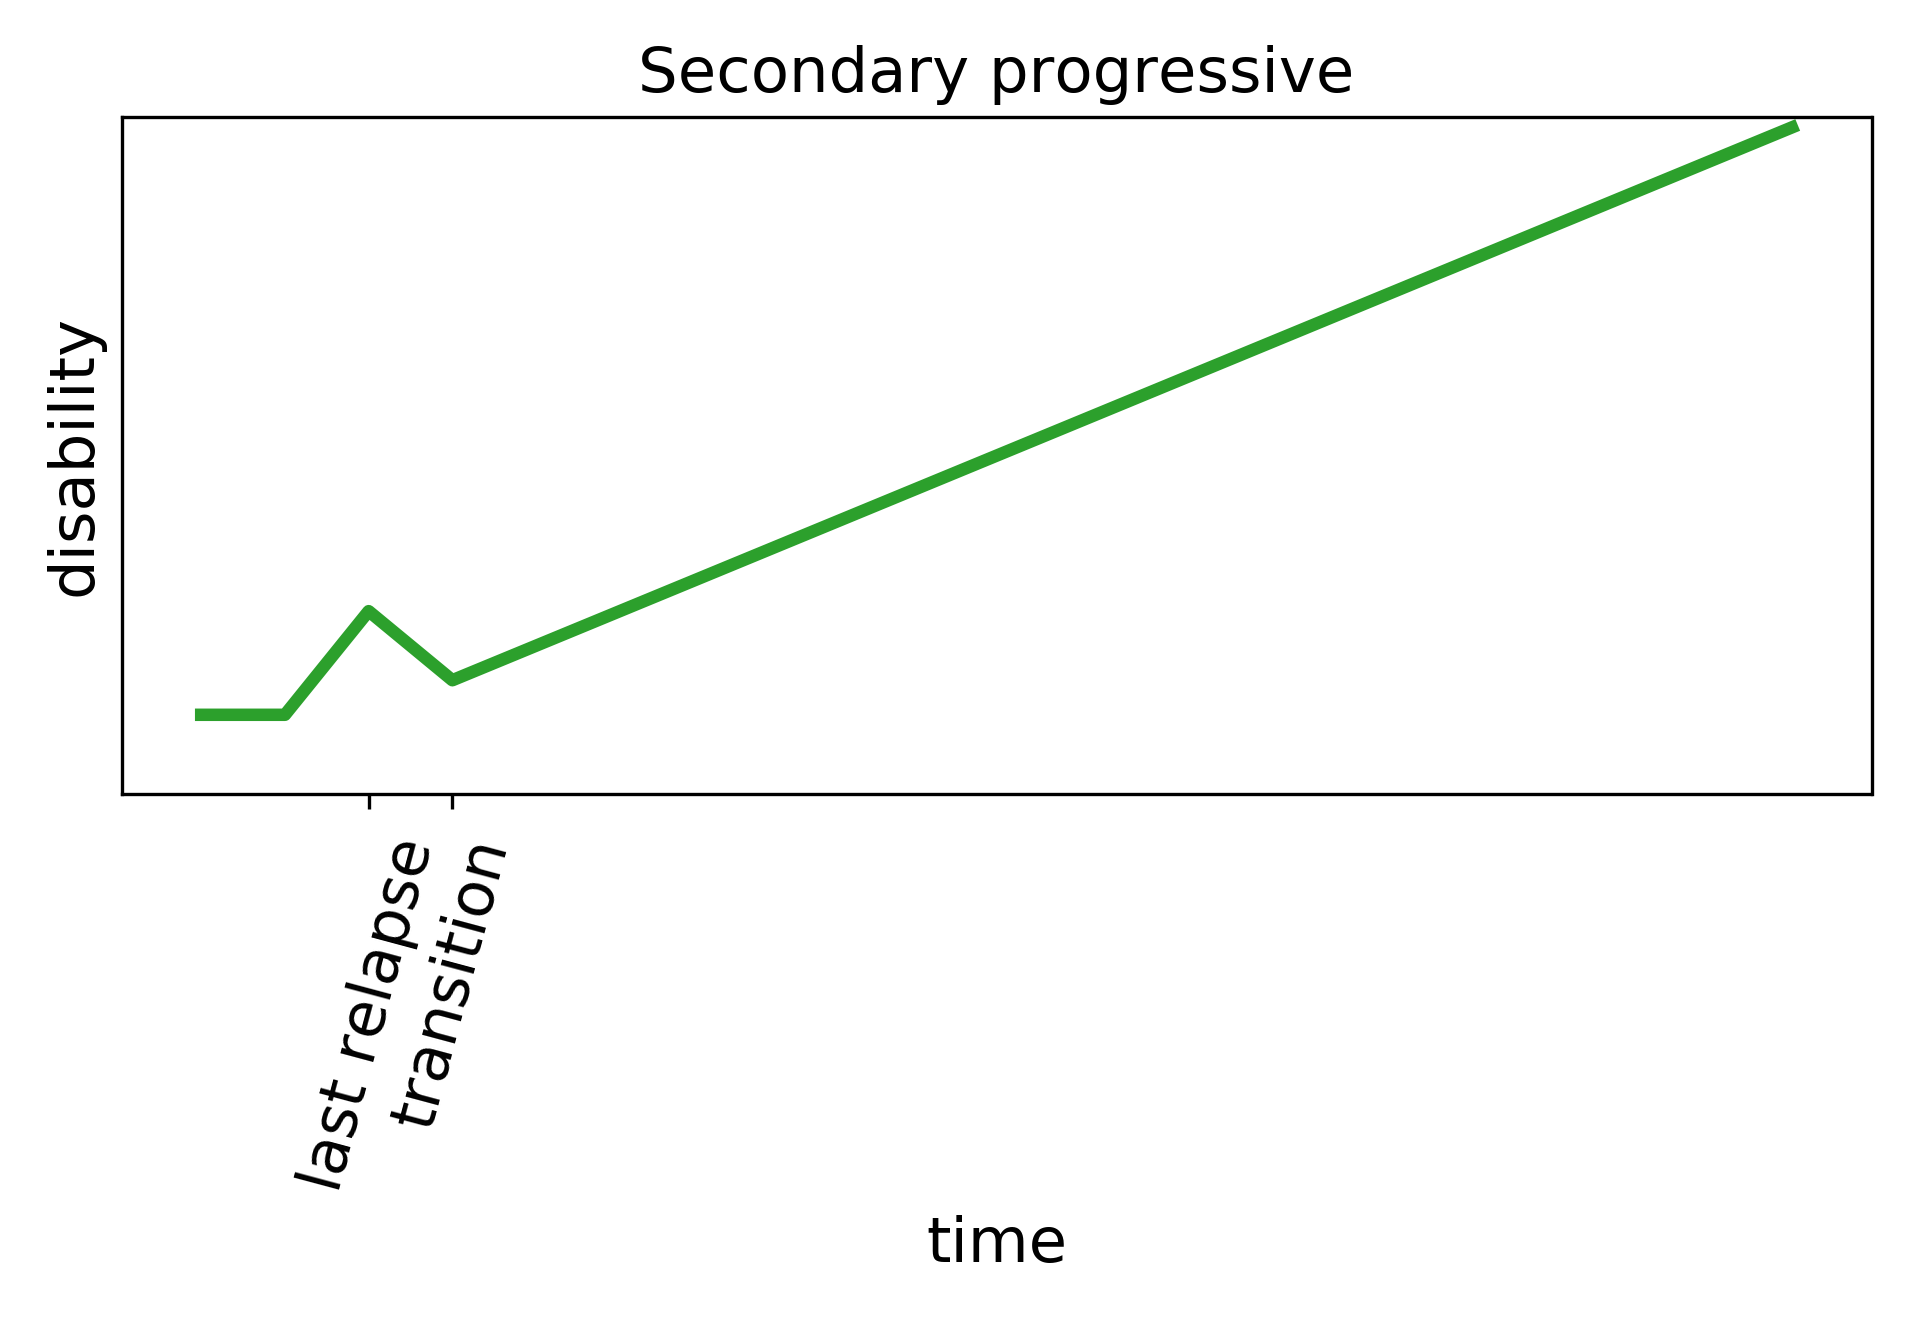
\includegraphics[width=0.5\textwidth]{part2/ms_mock_sp.png}
		\label{fig:ms_mock_sp}%
	}
	\hfill
	\subfloat[]{%
		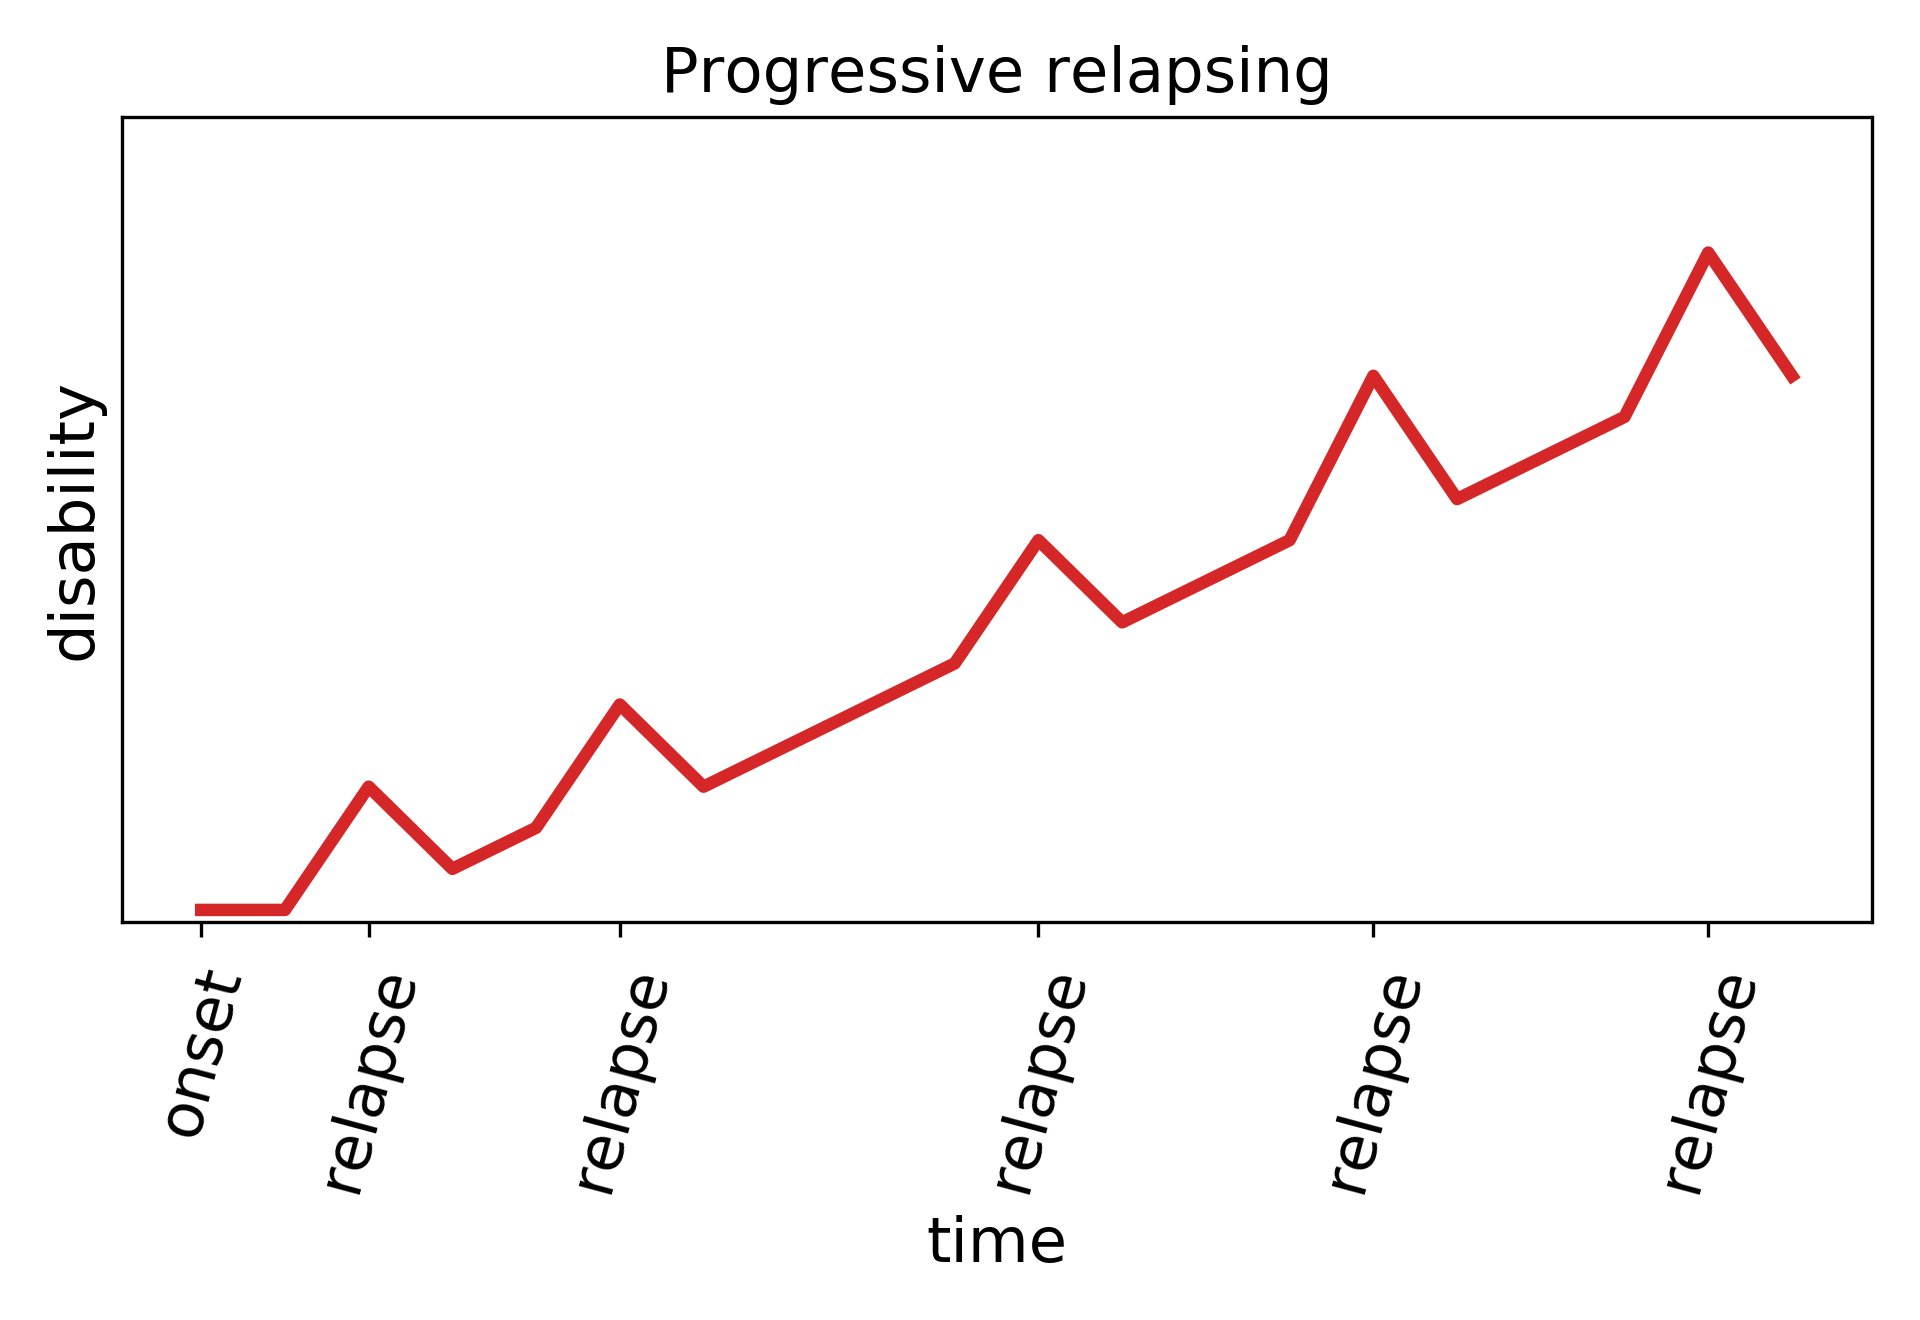
\includegraphics[width=0.5\textwidth]{part2/ms_mock_pr.png}
		\label{fig:ms_mock_pr}%
	}%
	\subfloat[]{%
		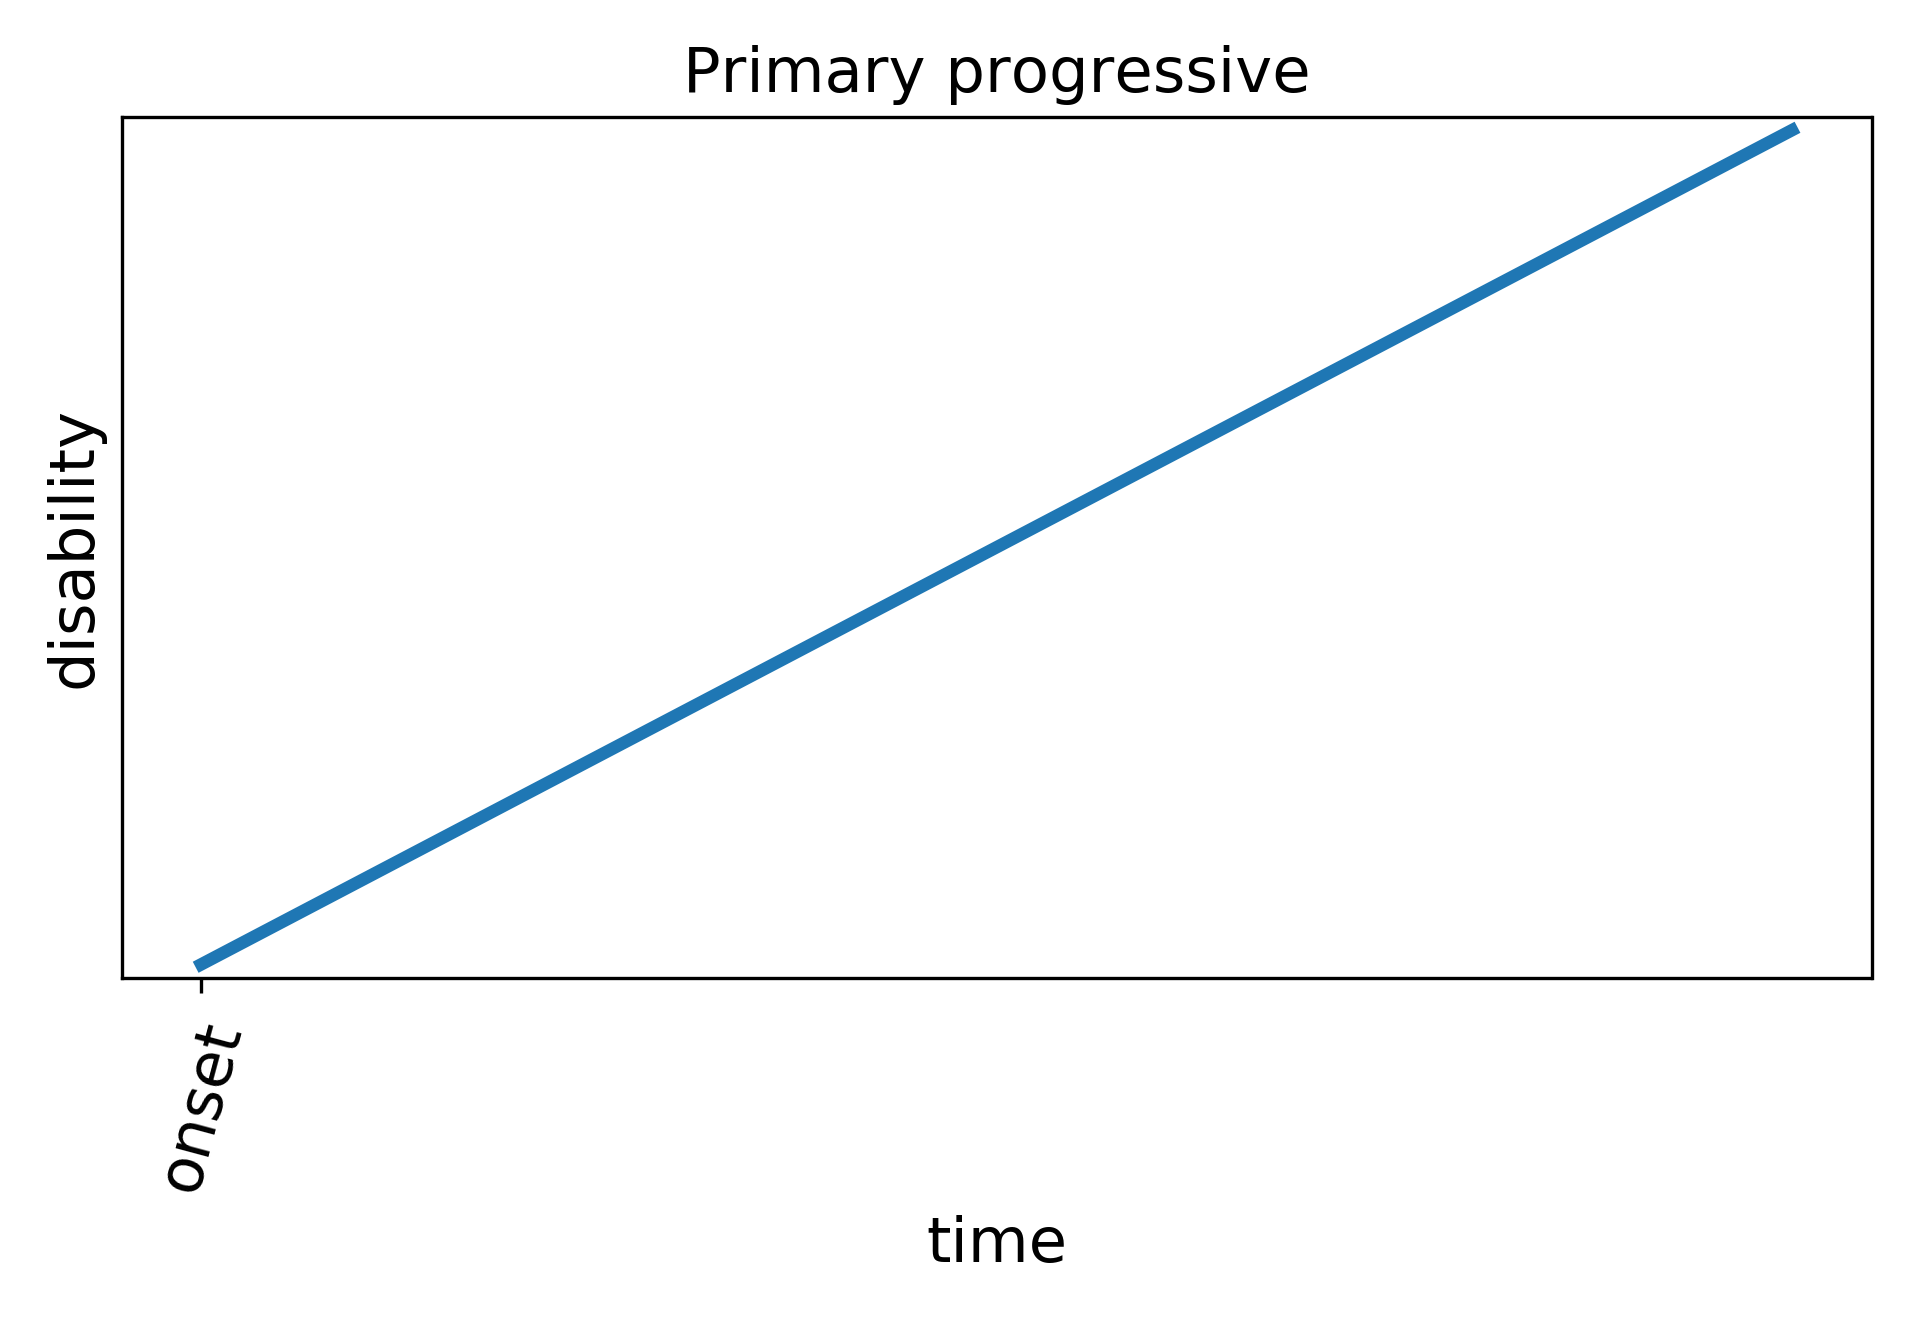
\includegraphics[width=0.5\textwidth]{part2/ms_mock_pp.png}
		\label{fig:ms_mock_pp}%
	}
	\caption{Disability evolution of the four main MS courses: panel (a) shows a prototypical \RR patient, characterized by time-limited attacks which may or may not leave permanent deficits; panel (b) shows \SP typical disability progression, that is steady with no more relapses; panel (c) represents a typical \PR disability evolution, which is characterized by steady disability progression from the onset; panel (d) shows a \PR patient; which has a steady disability progression from the onset with relapses.} \label{fig:ms_mock}
\end{figure}


% This form is characterized by clearly defined {\em relapses}, \ie  attacks of neurological worsening, followed by partial or complete recovery.
% and it takes only $14$ years on average for people to become unable to walk for $100$ meters unaided .
% Patients in \SP form experience a steady progress of the disease in absence of relapses, while patients in \PR form are characterized by both relapses and gradual worsening.

For this reason, the prediction of the transition from \RR to \SP is one of the most important methodological gaps that MS researchers are currently addressing.
The availability of a statistical model able to predict disease worsening is one of the major unmet needs that could significantly improve timeliness, personalization and, consequently, the efficacy of the treatments.
Nowadays, there are no clear clinical, imaging, immunologic or pathologic criteria to foresee the transition from \RR~to~\SP~\cite{lublin2014defining}. Several clinical factors relating to possible \SP course predictors have been identified~\cite{bergamaschi2015bremso, dickens2014type}.
However, as showed by~\cite{vukusic2003prognostic}, studies investigating on prognostic factors for MS course evolution generally suffer from two shortcomings: they
% However, such studies generally
report a high proportion of \RR patients not monitored enough to reach progressive course and they lead, to some extent, to contradictory results.
Currently, MS research mainly focuses on developing and assessing drugs and rehabilitative protocols for \RR patients disregarding progressive courses.

\section{\PCOs data collection}\label{sec:proms_data_collection}

In the recent past, researchers explored the potential role of Patient-Centered Outcomes (\ac{PCO}) to follow the progression of neurodegenerative diseases and to take timely decisions~\cite{black2013patient}. %~\todo{REF \cite{??}}.
%\PCOs usually consist in ordinal or categorical scaled questionnaires and self-reported measures.
\PCOs comprise self- and physician-administered tests, questionnaires and clinical scales consisting of either ordinal or categorical scaled answers.
As opposed to stressful, not frequently repeatable and expensive clinical exams, like magnetic resonance imaging or blood tests, \PCOs are patient-friendly and low-cost measures that could allow to investigate the individual changes and disease impact on several aspects such as physical, cognitive, psychological, social and well-being domains~\cite{fiorini2015machine}.
%.
To date, \PCOs are extensively used to assess general health status, to support diagnosis and monitor progress of disease and to quantify the patients' perception of the effectiveness of a given therapy or procedure \cite{nelson2015patient}.
Nevertheless, it is still unclear which are the most informative \PCOs and, contextually, whether they can be used as {\em predictors} for disease evolution.

%\todo{In our study, we propose a machine learning approach that, leveraging on \PCOs data, aims at
%forecasting the transition of PwMS from \RR to \SP and at providing insights on the most appropriate use of \PCOs.}
%In our study, we propose a machine learning approach that, leveraging on \PCO data, aims at predicting the temporal evolution of MS disease course providing insights on the most appropriate use of \PCOs.
%We resort to a vast category of predictive models, ranging from sparse regularization to ensemble and deep learning methods.
%These models are widely adopted in the biomedical context as they benefit from good generalization properties as well as they allow to address regression and classification problems within the same statistical and computational framework~\cite{lecun2015deep, qi2012random, nowak2011fused,  teramoto2009balanced, zou2005regularization}.
%azencott2013efficient

% \PCOs are low-cost and patient-friendly source of information that can be acquired over time in order to quantitatively assess patients' disease impact on several aspects of their life.

The biomedical data science challenge presented in this chapter is based on a \PCO dataset acquired from a cohort of PwMS progressively enrolled within an ongoing funded project \footnote{ethical review committee approval \textit{023REG2014} was obtained for this work}.

Each patient is evaluated every four months through the items of the \PCOs reported in Table~\ref{tab:proms} which cover physical, cognitive and psychosocial domains. A comprehensive description of the \PCOs involved in the study is presented below.


\begin{itemize}
	\item[] {\sc \textbf{MFIS}} This is a $21$-item self-reported questionnaire typically administered in $5$ to $10$ minutes. \MFIS provides an assessment of the effects of fatigue in terms of physical, cognitive, psychosocial functioning and it is considered a valuable tool by clinicians.
	
	\item[] {\sc \textbf{HADS}} This is a $14$-item self-reported questionnaire typically administered in $2$ to $6$ minutes which aims at detecting clinically significant symptoms of depression and anxiety in patients. \HADS consists in $7$ questions for depression and the remaining $7$ for anxiety.
	
	\item[] {\sc \textbf{LIFE}} This is an $11$-item self-reported questionnaire which investigates on patients quality of life. \LIFE can be typically administered in approximately $5$ minutes. To each of the $11$ items, the patient can assign an ordinal score $0,1,2$ which corresponds to "\textit{disagree}", "\textit{not sure}" and "\textit{agree}" answers.
	
	\item[] {\sc \textbf{OAB}} This is an $8$-item self-reported questionnaire which investigates on patients bladder control. \OAB can be administered in approximately $5$ to $8$ minutes and it is a reliable tool to investigate on possible stress or discomfort lead by unexpected urinary urgencies that patients may experience during day or night.
	
	\item[] {\sc \textbf{EDINB}} This $10$-item self-reported questionnaire can be used to assess dominance of a person's right/left hand during daily activities. The items are very straightforward, so \EDINB can be administered in $3$ to $5$ minutes.
	
	\item[] {\sc \textbf{ABILH}} This is a $23$-item self-reported questionnaire which can be used to measure hand ability in adults with upper limb impairments. \ABILH assesses a person's ability to manage daily activities that require the use of the upper limbs, whatever the strategies involved. \ABILH is usually administered in $5$ to $10$ minutes.
	
	\item[] {\sc \textbf{FIM}} This is $19$-item clinical scale assessing the amount of assistance required for the patient to carry out activities of daily living. \FIM is typically administered by trained examiner in $35$ to $40$ minutes and it covers both motor and cognitive domains.

	\item[] {\sc \textbf{MOCA}} This is an $11$-item clinical scale assessing several cognitive domains such as short-term memory recall, visuospatial abilities, phonemic fluency, attention, concentration and so on. \MOCA is typically administered in less than $10$ minutes.
	
	\item[] {\sc \textbf{PASAT}} This clinical scale is a measure of cognitive function that assesses patients' auditory processing speed and flexibility,  as well as their calculation ability. It can be administered in $10$ to $15$ minutes and it consists in audio stimuli in which single digits are presented every $3$ seconds. The patient is asked to add each new digit to the one immediately prior to it. \PASAT must be administered by trained examiner.
	
	\item[] {\sc \textbf{SDMT}} This clinical scale is a test for organic cerebral dysfunctions. This test simply involves a substitution task: using a reference key the patients has few seconds to pair specific numbers with specific geometric measures.
	\SDMT is typically administered by trained examiner in less than $5$ minutes.
	
	\item[] {\sc \textbf{EDSS}} This is probably the oldest assessment instrument for MS. \EDSS is based on a neurological examination consisting of $7$-items. Each item rates a different function, all the items are then combined in the final \EDSS score which is an ordinal scale ranging from $0$ (normal neurological examination) to $10$ (death due to MS), in half-point increment. The use of \EDSS in modern MS assessment is somewhat controversial. Although usually adopted as an index of the disability level, \EDSS focuses mainly on deambulation disability without taking into account other aspects that could impact patient disability, such as upper limb or cognitive functions~\cite{meyer2014systematic, uitdehaag2014clinical}.
	
	
\end{itemize}

\PCO data are intrinsically noisy due to the subjectivity of self-reported measures provided by the patients that can be influenced by personal feelings and opinions. In order to ameliorate this issue, $4$ questionnaires out of $10$ are administered by medical staff which is trained to keep a homogeneous level of evaluation.

In our analysis we considered all the \PCOs reported in Table~\ref{tab:proms} except \EDSS.
%\todo{other comments here?}

% The model considered all the \PCOs except \EDSS, that is a physician reported outcome that, although usually adopted as an index of the disability level, exclusively depends on the deambulation for scores greater than 4, consequently not taking into account the other aspects impairing the patient.

\begin{table}[htb]
	\center
	\footnotesize
	\begin{tabular}{l|l|l}%{@{} l*{4}{l} @{}}
		\toprule
		Acronym & Full name & Reference \\
		\midrule
		\MFIS & Modified fatigue impact scale & \cite{flachenecker2002fatigue}\\
		\HADS & Hospital anxiety and depression scale &  \cite{honarmand2009validation}\\
		\LIFE &  Life satisfaction index &  \cite{franchignoni1999life}\\
		\OAB & Overactive bladder questionnaire & \cite{cardozo2014validation}\\
		\EDINB &  Edinburgh handedness inventory & \cite{oldfield1971assessment} \\
		\ABILH &  Hand ability index & \cite{arnould2012can} \\
		\midrule
		\FIM &  Functional independence measure  &\cite{granger1990functional}\\
		\MOCA &  Montreal cognitive assessment & \cite{dagenais2013value}\\
		\PASAT &  Paced auditory serial addition task & \cite{aupperle2002three} \\
		\SDMT &  Symbol digit modality test  & \cite{parmenter2007screening}\\
		\EDSS & Expanded disability status scale & \cite{kurtzke1983rating}\\		\bottomrule
	\end{tabular}
	\caption{The set of available \PCOs.
		The first $6$ are self-reported, while the last $5$ are administered by trained medical staff.
		In our analysis all \PCOs were used, with the exception of \EDSS.
		% The set of clinically validated questionnaires available for this work. All questionnaires were used to predict the disease course evolution with exception of \EDSS. The answers to the first $6$ questionnaires are completely self-reported, while the last $5$ are administered by trained medical staff.
	}\label{tab:proms}
\end{table}


% we focus on the use of $10$ of the clinically validated questionnaires reported in Table~\ref{tab:proms}. Each questionnaire consists of a different number of items testing the capabilities of the patients in different domains, such as physical, cognitive or psychosocial.
% Moreover, the set of variables considered by our
The collected \PCO dataset comprises additional information such as:
\begin{enumerate*}[label=\roman*)]
	\item number of relapses in the last four months (NR),
	\item educational level expressed in terms of total years of education (EDU),
	\item height (H) expressed in $\text{cm}$ and
	\item weight (W) expressed in $\text{kg}$.
\end{enumerate*}
Moreover, a neurologist assigns to each patient the corresponding disease course. The global distribution of MS types across time points is depicted in Figure~\ref{fig:PPRRSP}.

% \todo{@AISM: add here the motivations that lead us to exclude \EDSS from the analysis.}

%%%%%%%% EDA %%%%%%%%
\section{\PCOs exploratory data analysis} \label{sec:aism_eda}


 \begin{figure}[]
	\centering
	\subfloat[]{%
		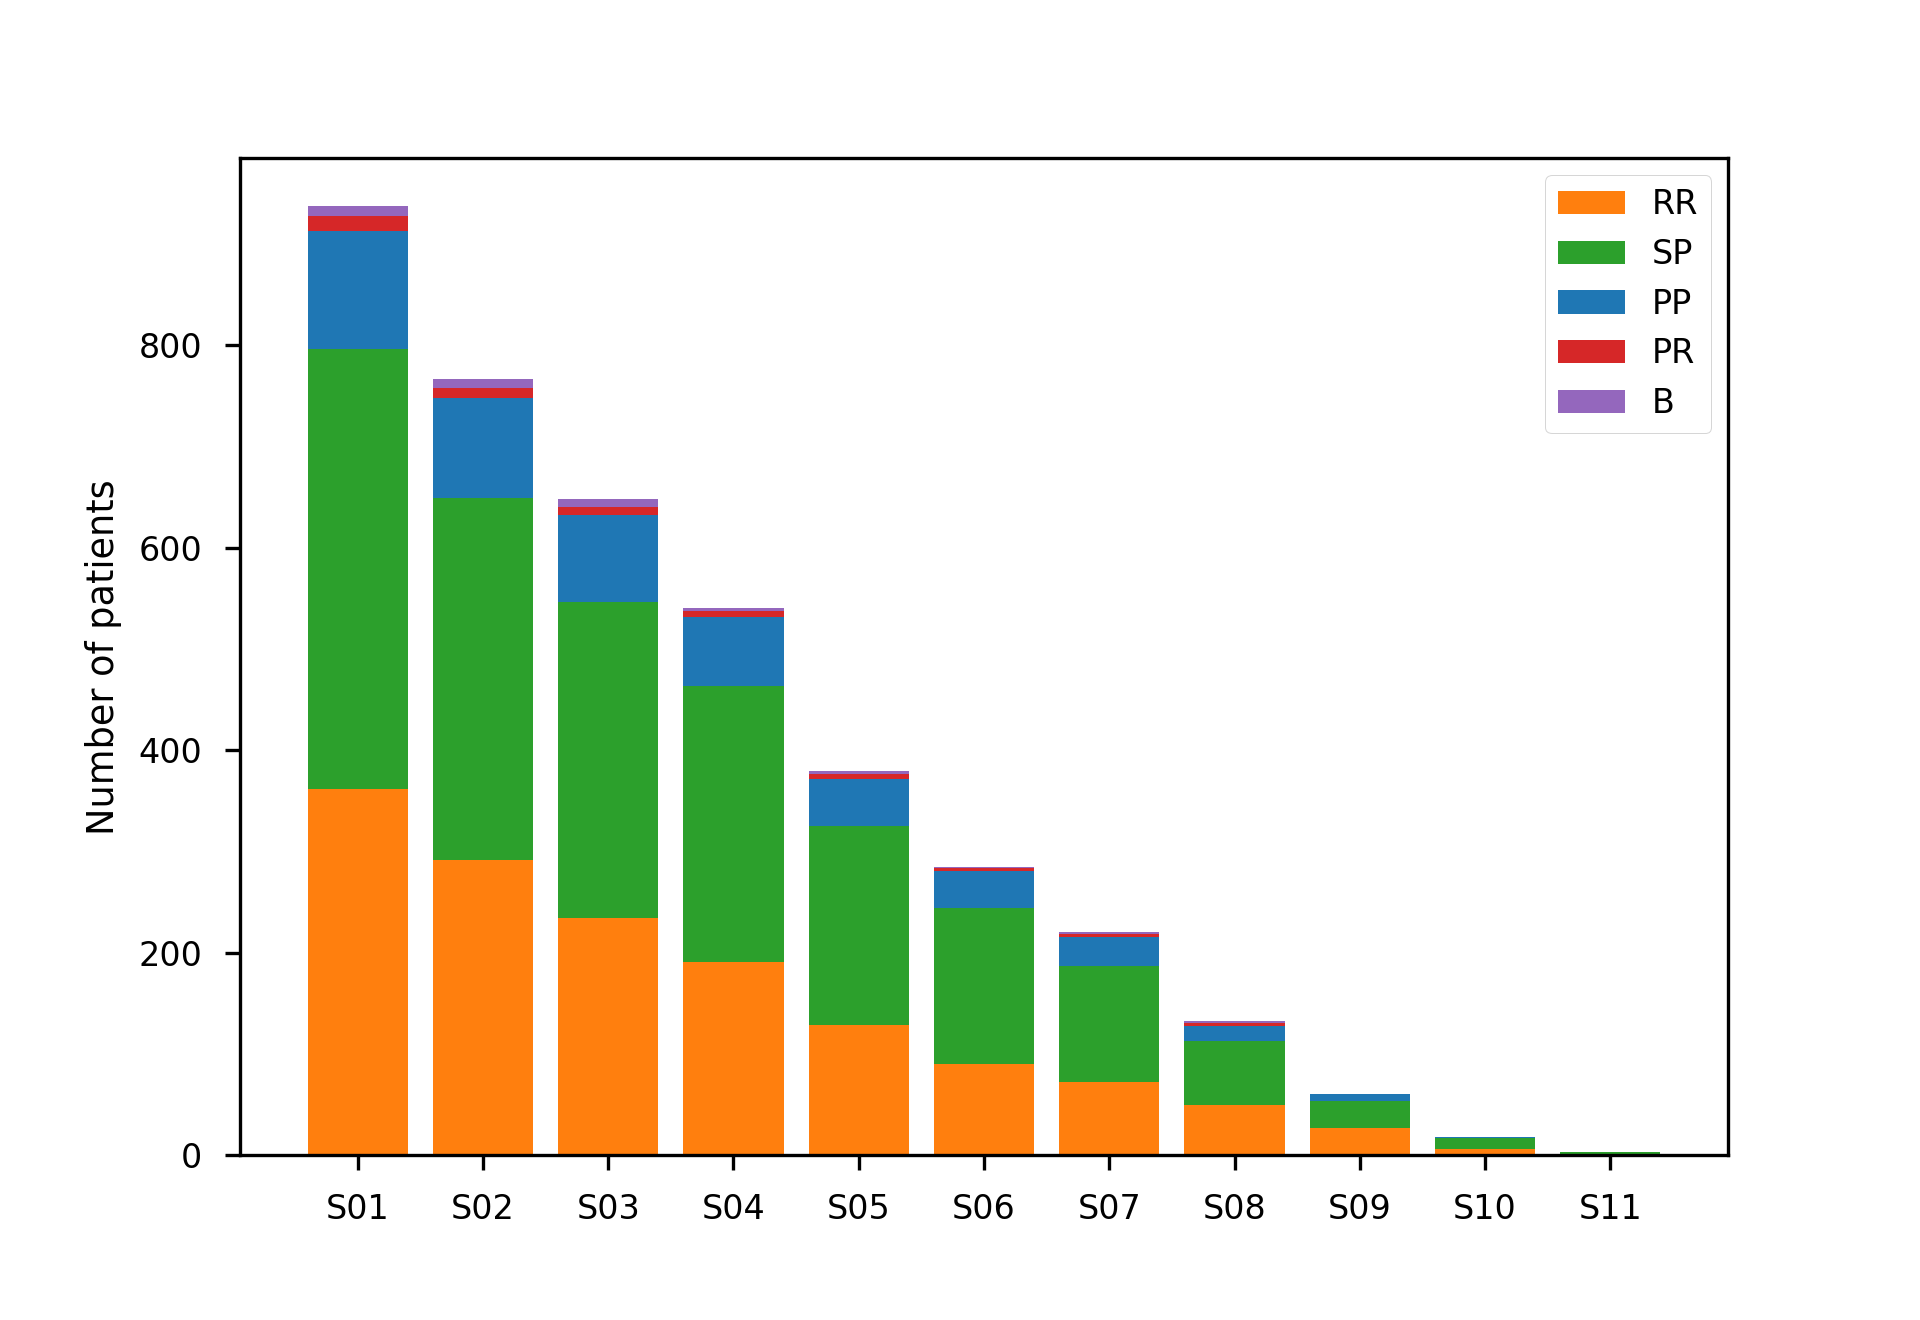
\includegraphics[width=0.5\textwidth]{part2/ms_bars.png}
		\label{fig:patients}%
	}%
	%	\hfill%
	\subfloat[]{%
		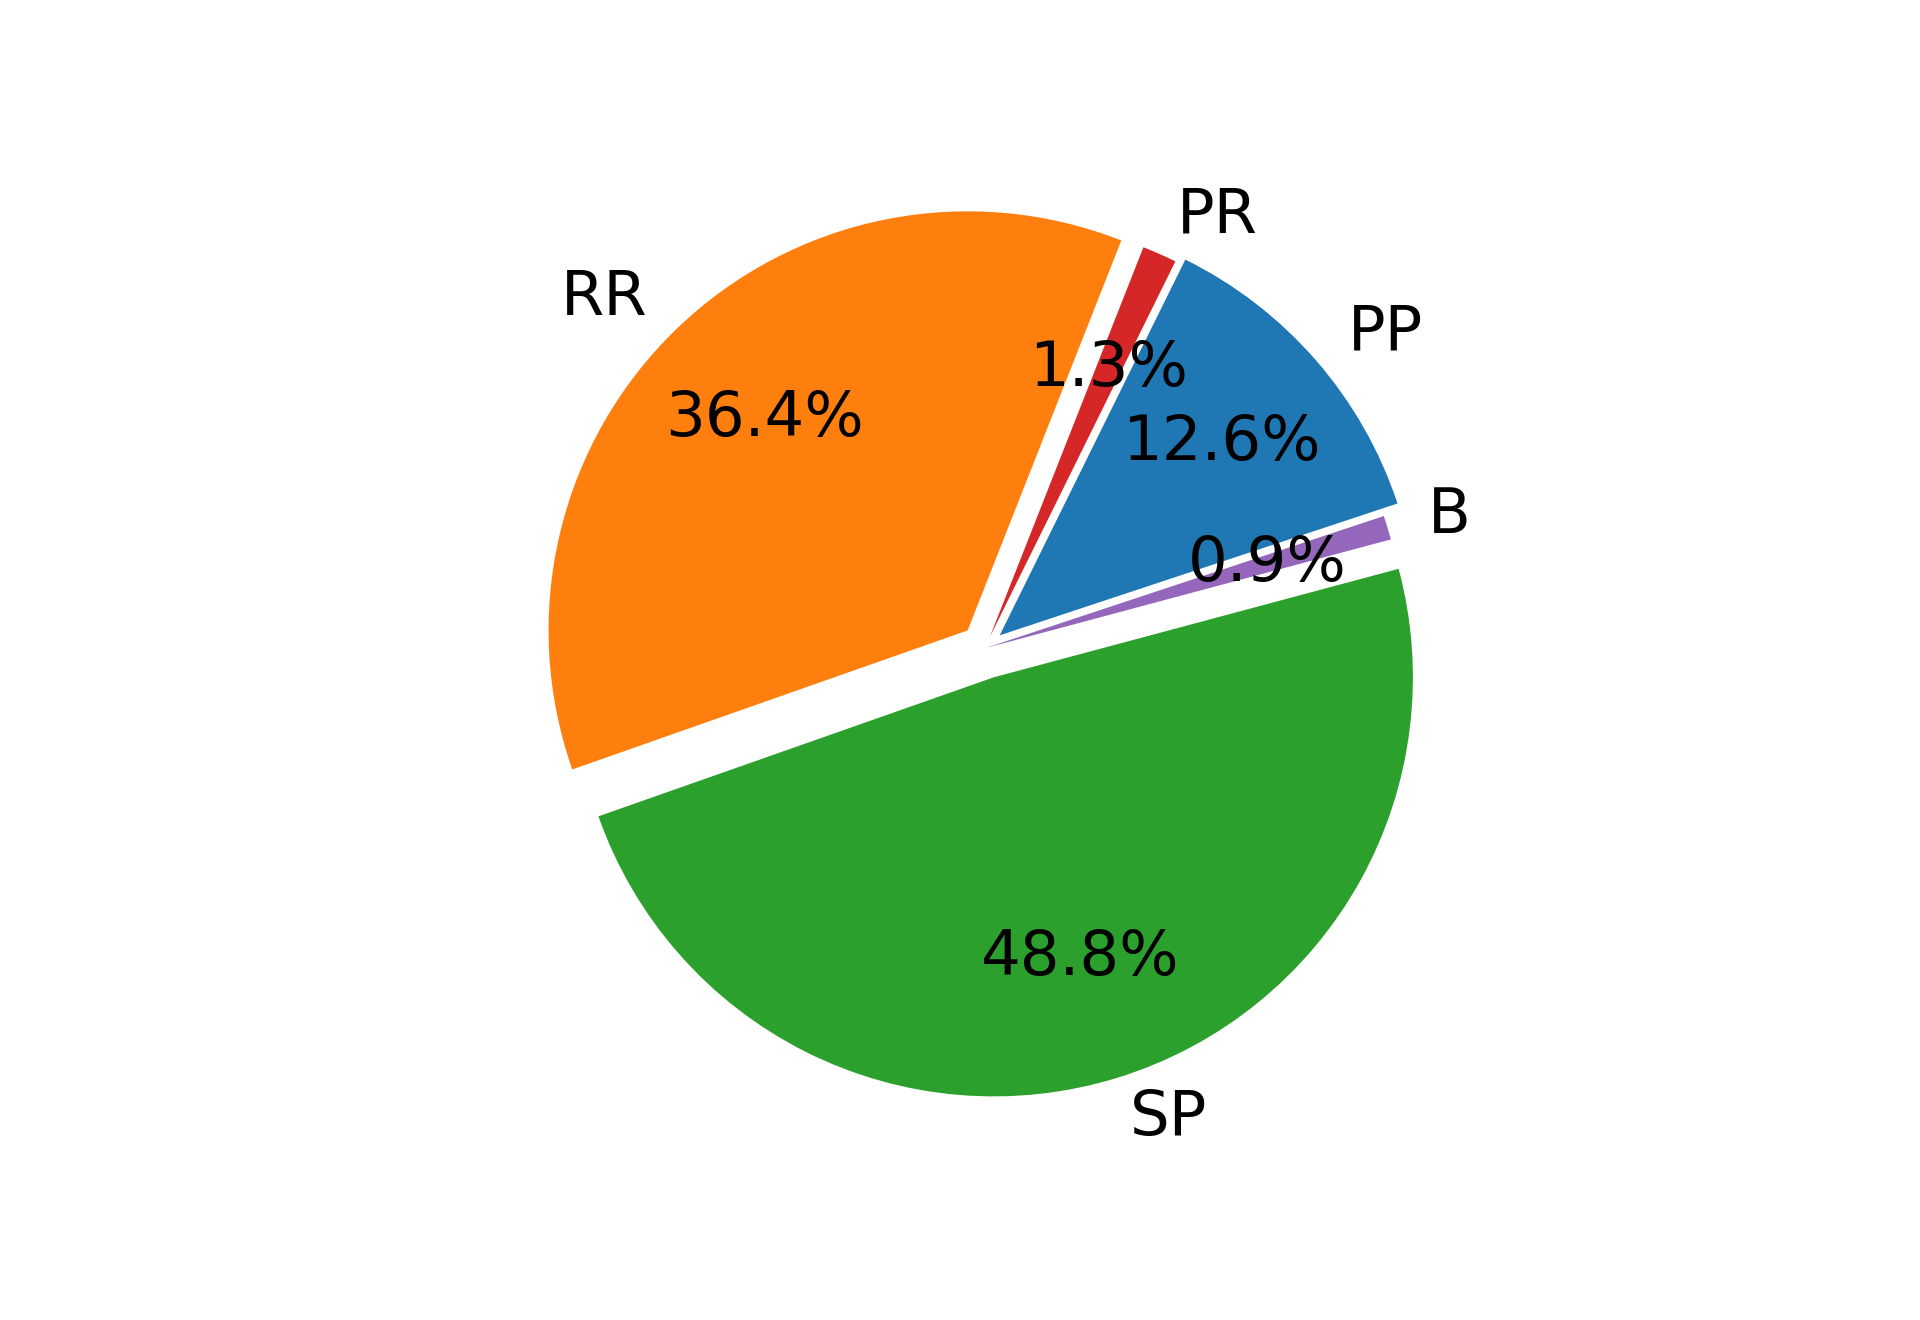
\includegraphics[width=0.5\textwidth]{part2/ms_pie.png} \label{fig:PPRRSP}
	}%
	\caption{An overview of the \PCO dataset used in this study. The left panel (a) shows a bar chart of the number of MS patients in each disease form  at different examinations. The right panel (b) presents a representation of the distribution of the total amount of acquisitions ($3991$), divided according to the disease form.}\label{fig:data}
\end{figure}


%In this work we focus on detecting the \RR to \SP prediction, hence the patients in \PR and \PP form will not be taken into account.

In this work we analyze \PCOs data acquired every four months from a cohort of MS patients enrolled in a funded study.
Currently, we have collected data for $11$ examinations and, as patients enrollment is still ongoing,  the number of individuals for each time point is successively decreasing
Our dataset comprises a grand total of $3991$ patients, with $1451$ \RR, $1947$ \SP, $503$ \PP, $53$ \PR and $37$ benign cases.
Each sample of the dataset is represented by a vector containing the $145$ predictors summarized in Table~\ref{tab:proms}.
As the missing data ratio amounts to $1.61\%$ of the entire dataset, we resort to the $k$-nearest neighbor data imputing strategy (with $k=5$) proposed in~\cite{troyanskaya2001missing}.

Analyzing \PCO data is challenging from several respects.
For instance, items belonging to different questionnaires are encoded with numerical values in different ranges.
As an example, the items of the \MFIS questionnaire have ordinal scale values in $[0-4]$, whereas the \SDMT outcome is the global number of correctly answered items of the test (max $110$) and the \EDINB test consists in $10$ categorical items measuring the dominance of right or left hand in the activities of daily living.
To tackle such issues, in this EDA we opted for a preliminary data preprocessing of the ordinal answers and a binary one-hot-encoding of the categorical ones, the latter increases the dimensionality of the samples, leading to $d=165$ variables in the dataset.
The adopted data preprocessing strategy, namely min-max scaling, consists in casting each feature $x^j$ in the a fixed range, \ie $x^{j'} \in [0, 1]$. The min-max scaling is obtained by the transformation in Equation~\eqref{eq:minmax}.
\begin{equation} \label{eq:minmax}
	x^{j'} = \frac{x^j - \min(x^j)}{\max(x^j) - \min(x^j)}
%	X_std = (X - X.min(axis=0)) / (X.max(axis=0) - X.min(axis=0))
\end{equation}
The effect of the data preprocessing on the ordinal input variables is visually represented in Figure~\ref{fig:ms_boxplots}. As we can see, this preprocessing step allows to compare more easily the input features.

\begin{figure}[]
	\centering
	\subfloat[]{%
		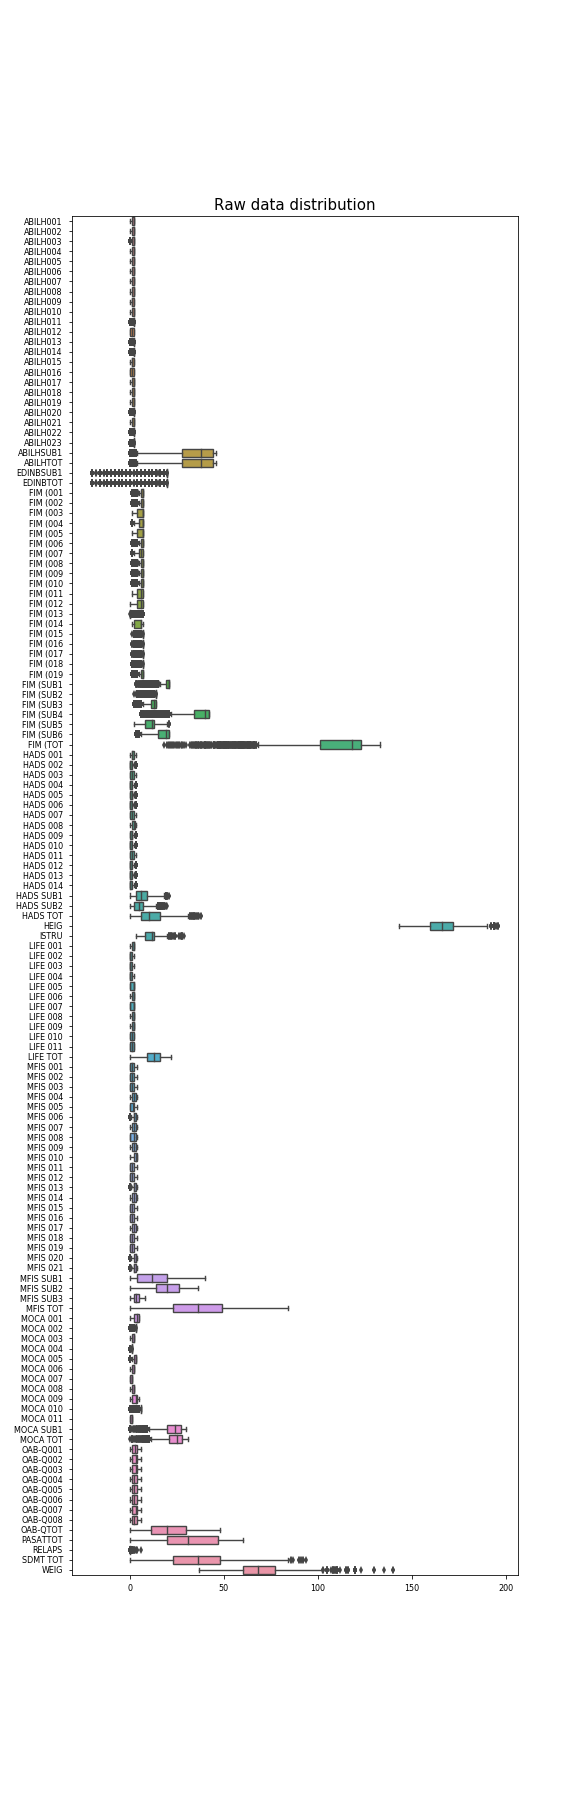
\includegraphics[trim={0 6cm 0 6cm}, width=0.5\textwidth]{part2/ms_raw_boxplot.png}
		\label{fig:ms_boxplots_pre}%
	}%
	%	\hfill%
	\subfloat[]{%
		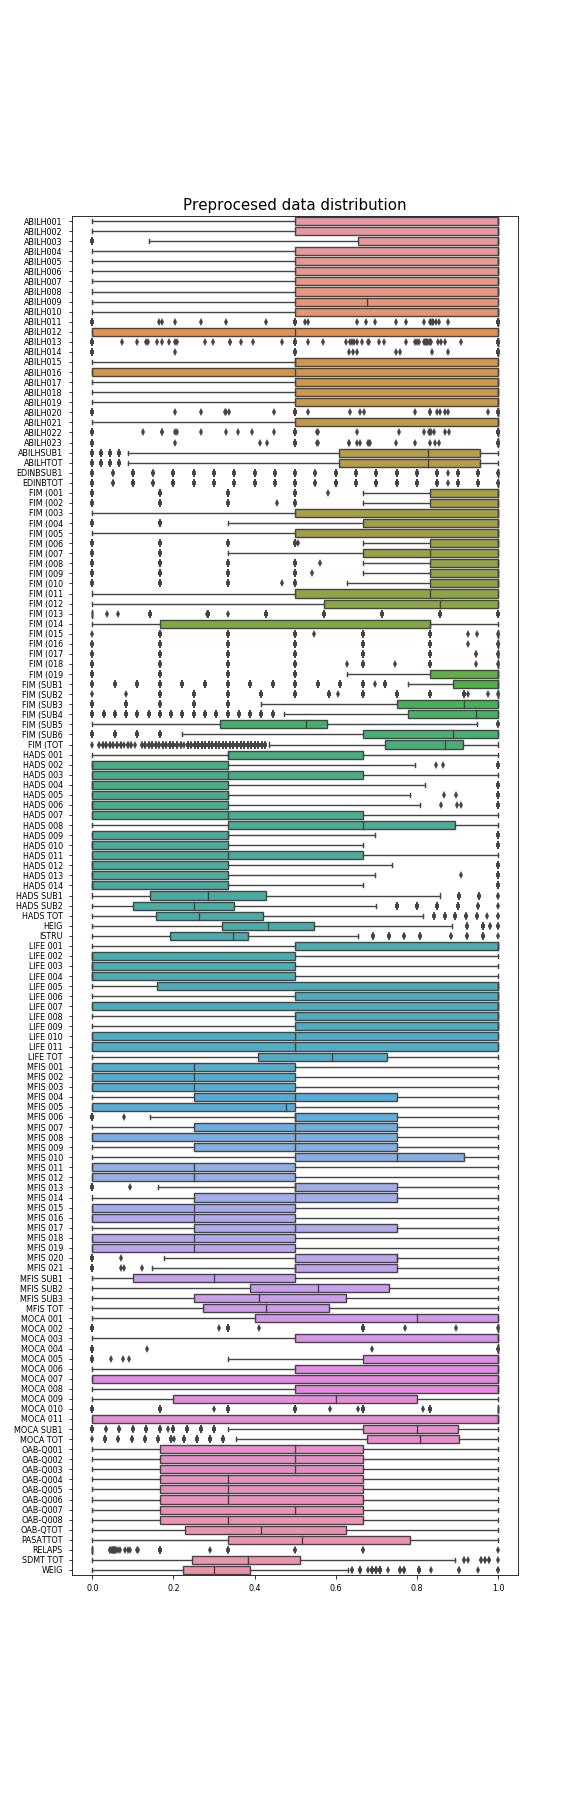
\includegraphics[trim={0 6cm 0 6cm}, width=0.5\textwidth]{part2/ms_mm_boxplot.png} \label{fig:ms_boxplots_post}
	}%
	\caption{The effect of the data preprocessing on the input ordinal \PCOs. The left panel (a) shows the distribution of the raw collected variables, whereas the right panel (b) shows the distribution of the same variables after the preprocessing step.}\label{fig:ms_boxplots}
\end{figure}

Furthermore, we try to decrease the dimensionality of the collected samples in order to visually inspect the data. To this aim, we project the data in a 3D space with linear PCA and Isomap (see Section~\ref{sec:dimred}).
These algorithms are sensitive to outliers, which we expect to affect our dataset. Therefore, we follow a preliminary isolation forests-based anomalies detection and removal as described in~\cite{liu2008isolation, liu2012isolation}.
The obtained scatter plots are shown in Figure~\ref{fig:ms_3dscatterplot}.
As we can see, both the obtained projections hint some sort of class separation between \RR and \SP subjects, while the same conclusion cannot be drawn for the other classes. Moreover, considering only the first three principal components, PCA explains only the $37.4\%$ of the variance of the dataset. This suggests that more information, which may be useful for classification purposes, is spread across several input variables.
%in this dataset the low dimensionality projection and visualization is not insightful. From the scatter plots in Figure~\ref{fig:ms_3dscatterplot} a clear class separation cannot be firmly observed.

\begin{figure}[h!]
	\centering
	\subfloat[]{%
		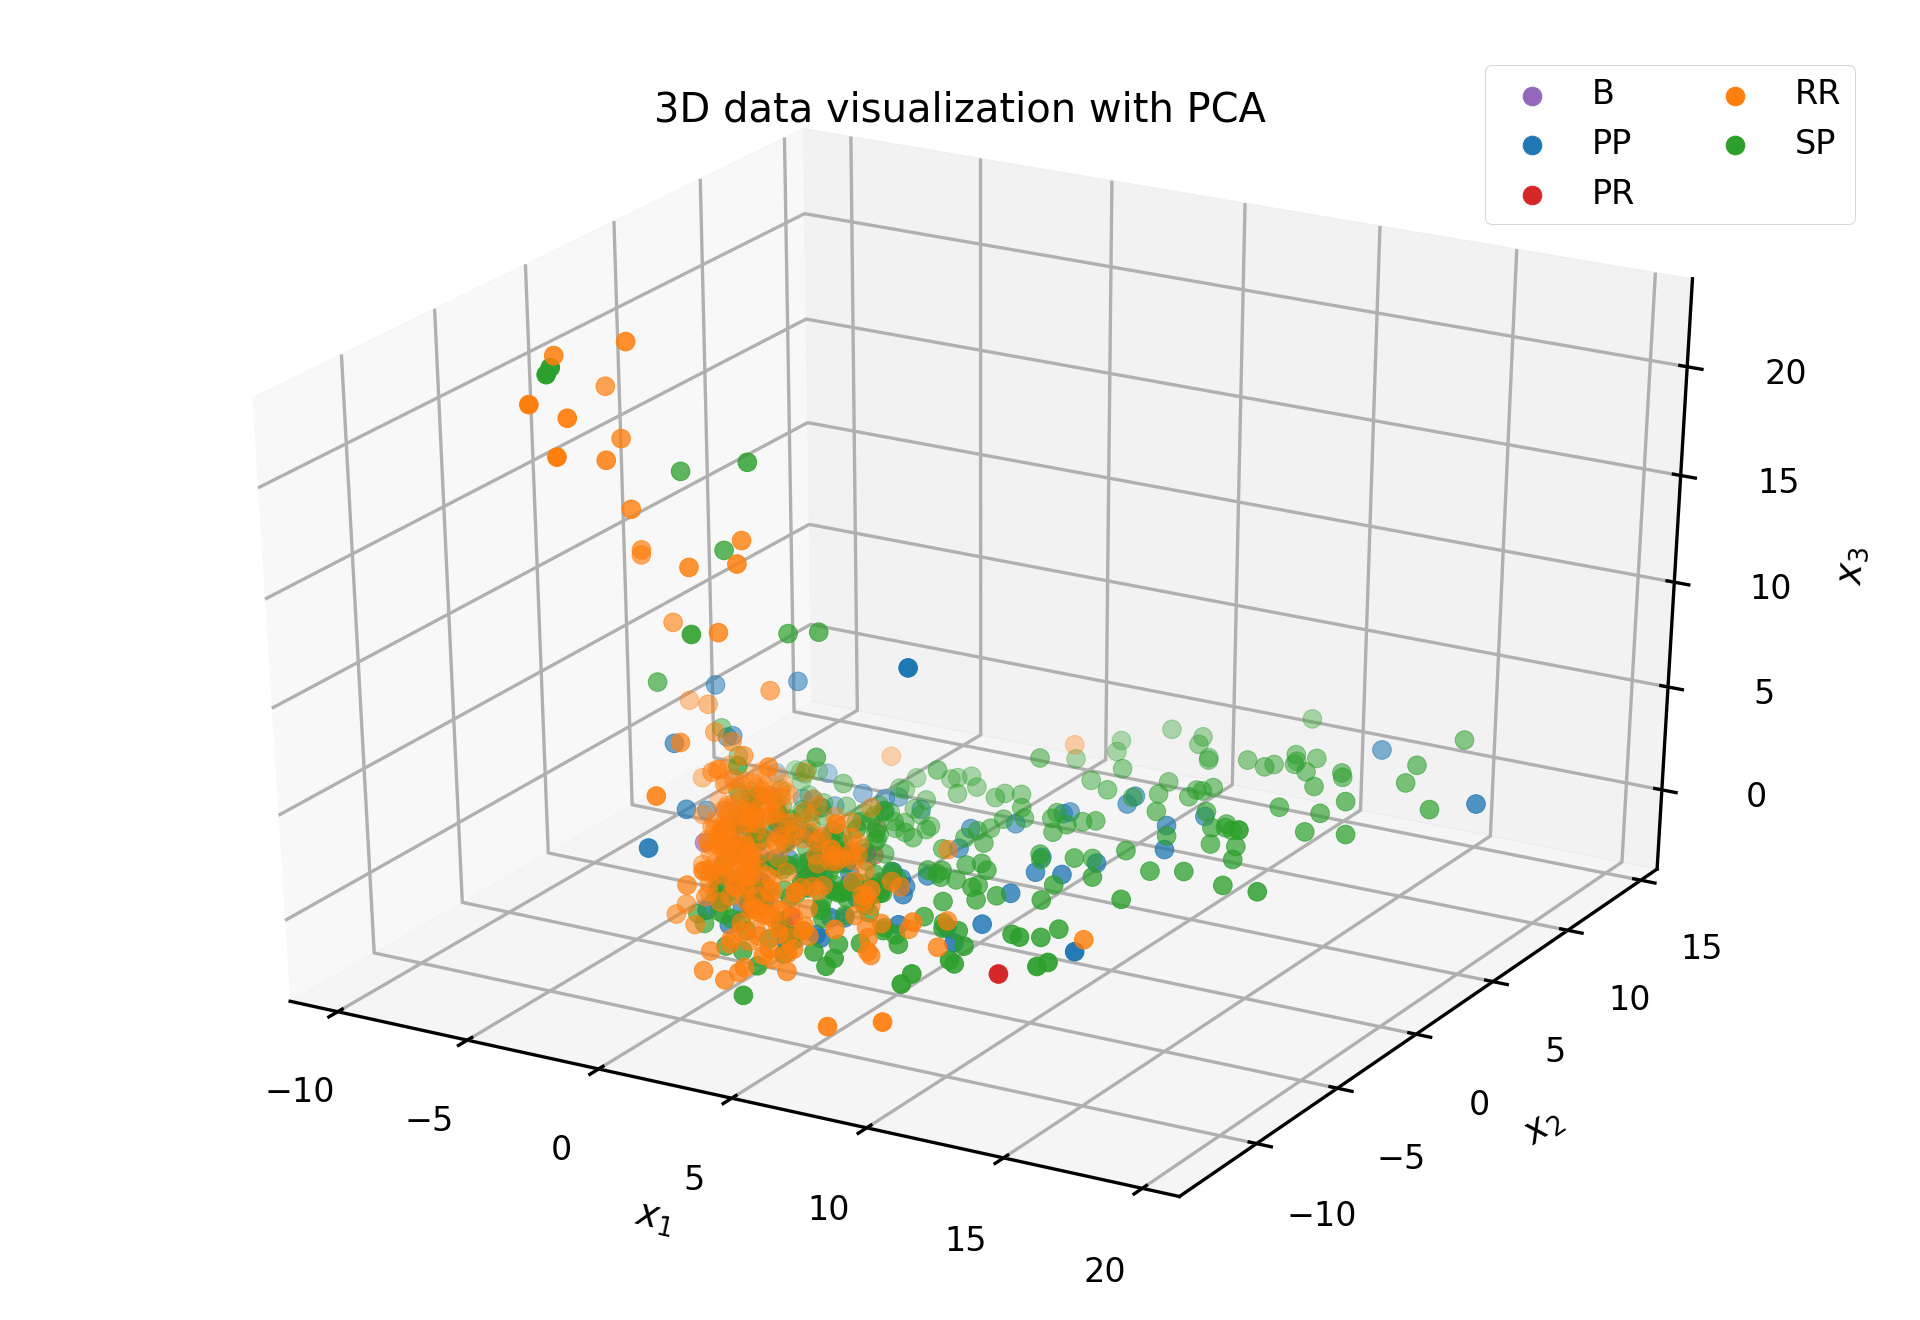
\includegraphics[width=0.5\textwidth]{part2/ms_pca.png}
		\label{fig:ms_ms_pca}%
	}%
%	\hfill
	\subfloat[]{%
		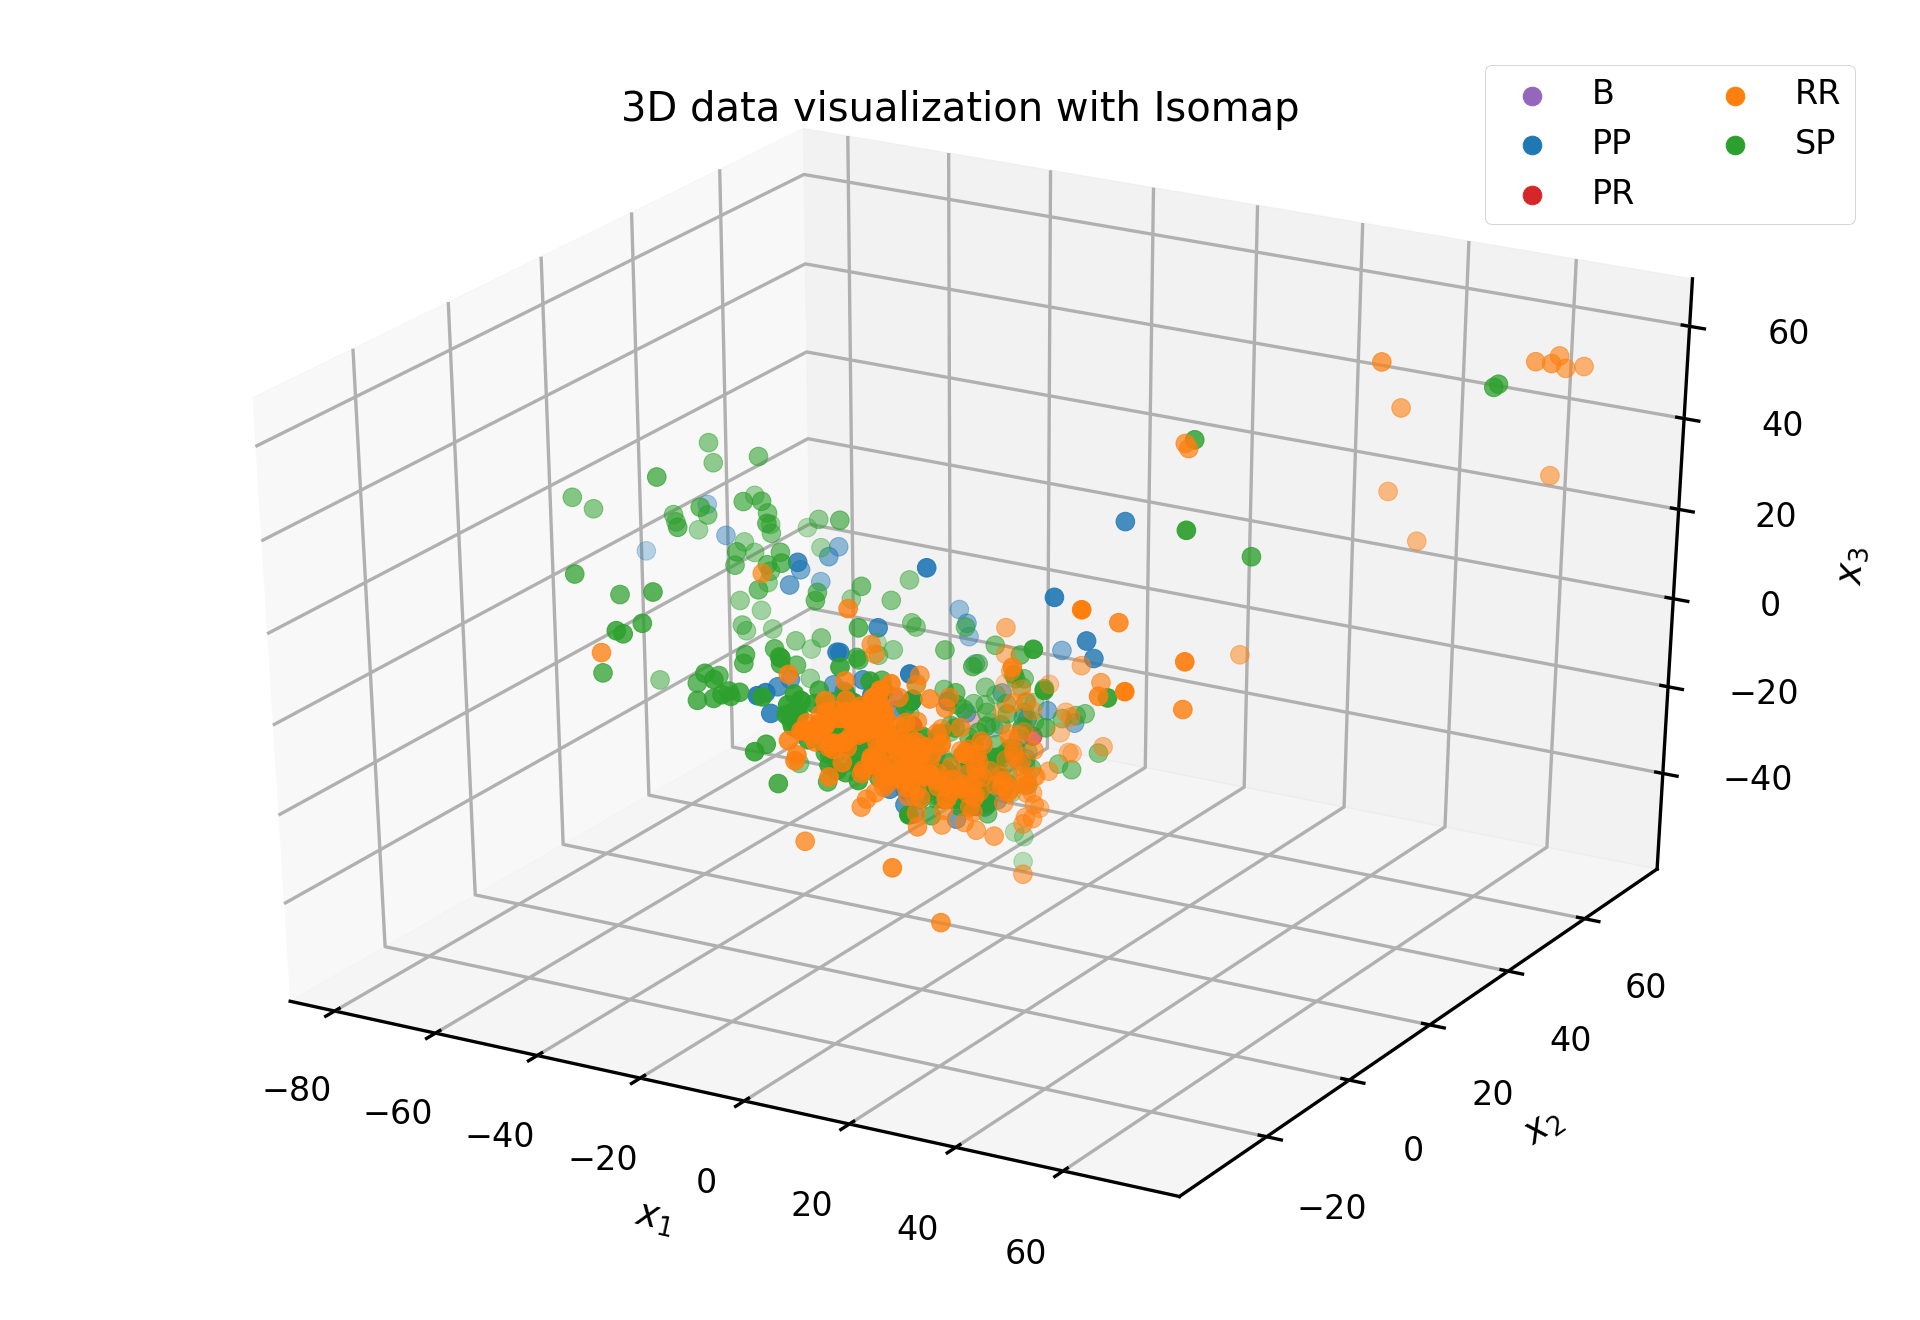
\includegraphics[width=0.5\textwidth]{part2/ms_isomap.png}
		\label{fig:ms_ms_isomap}%
	}
%	\subfloat[]{%
%		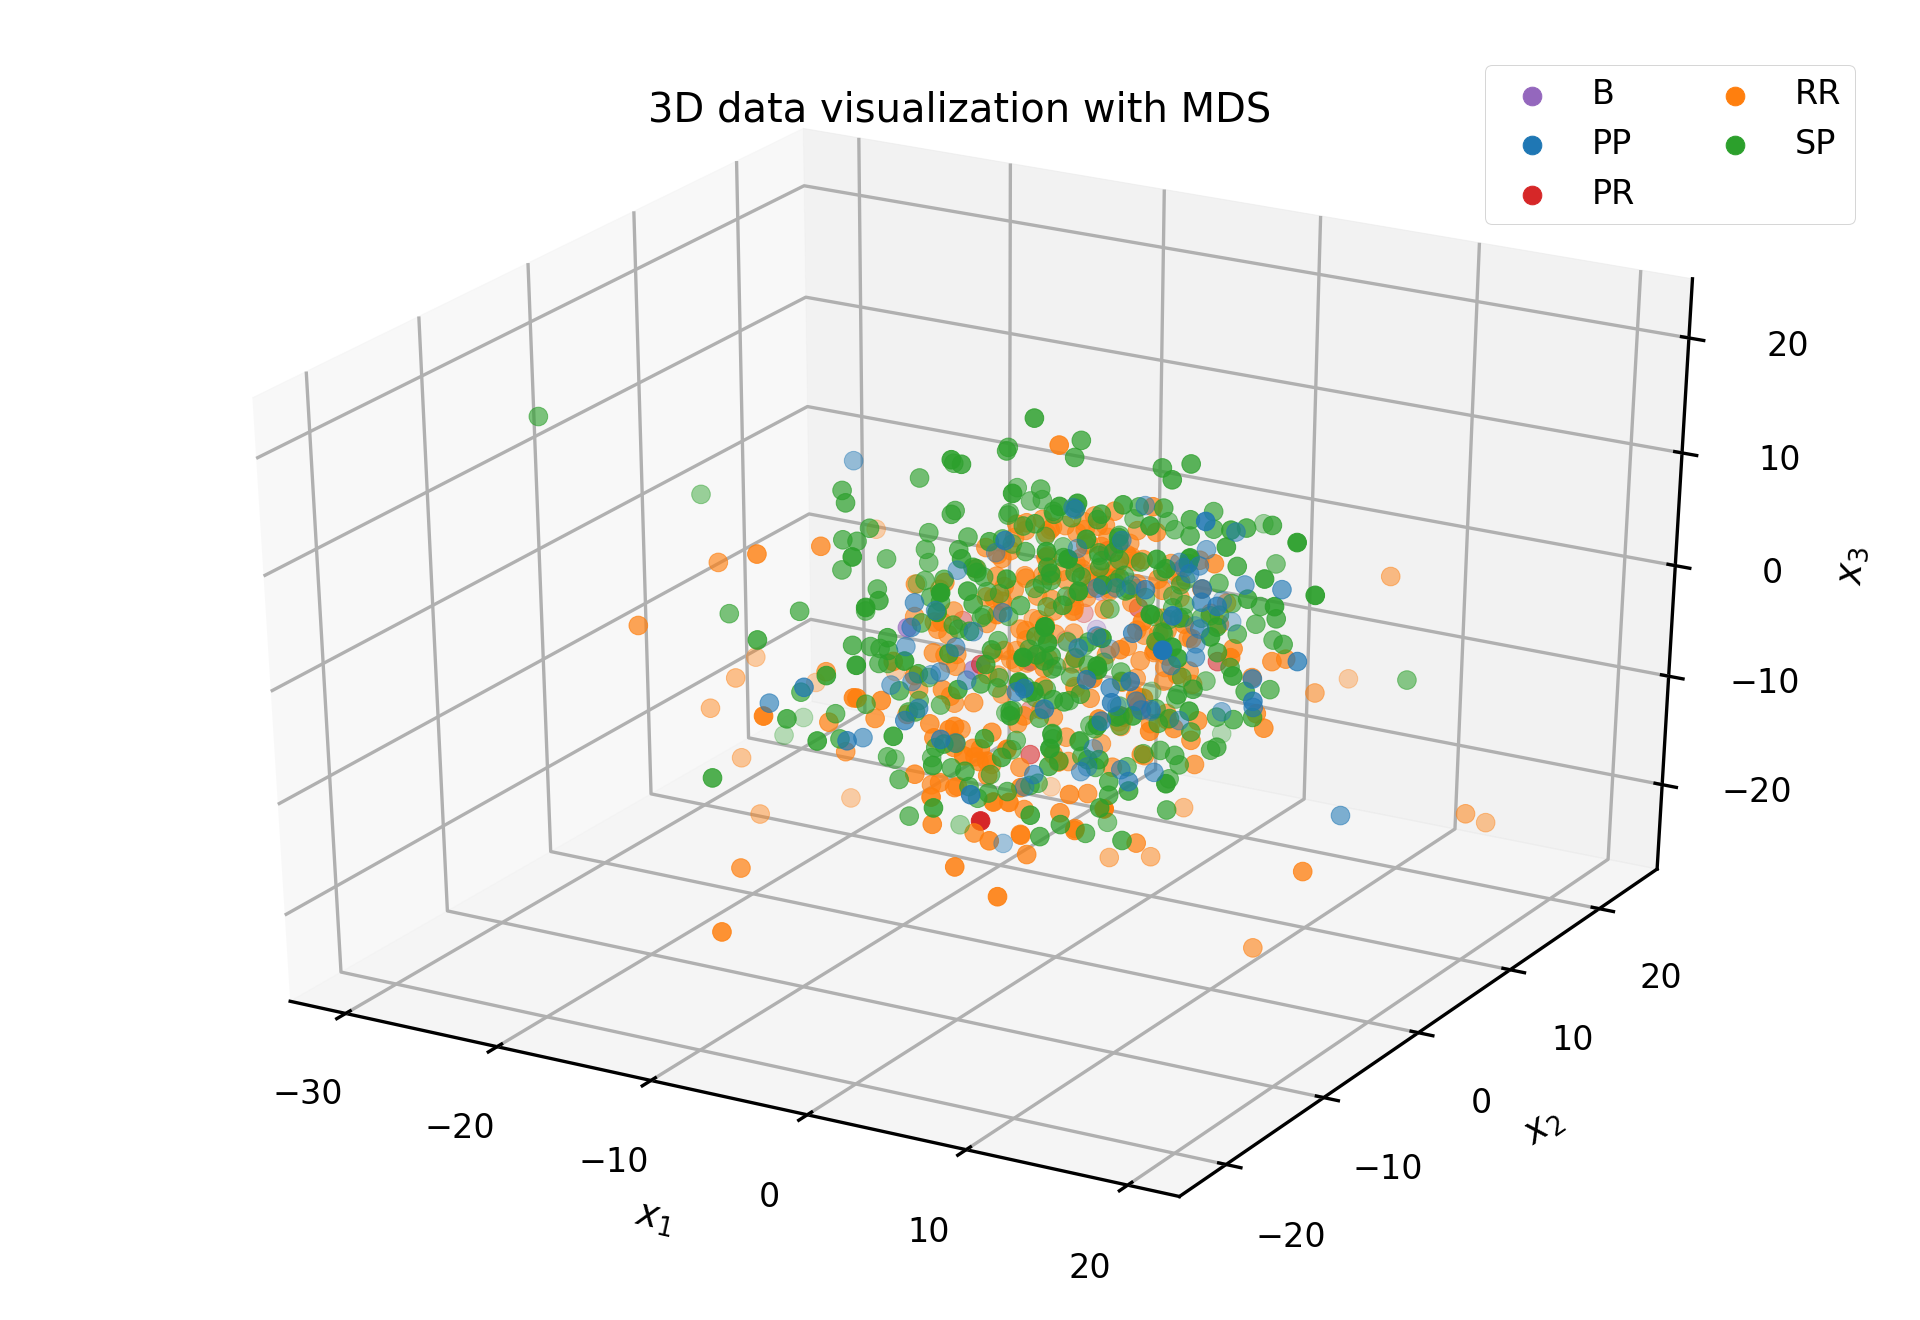
\includegraphics[width=0.5\textwidth]{part2/ms_mds.png}
%		\label{fig:ms_ms_mds}%
%	}%
%	\subfloat[]{%
%		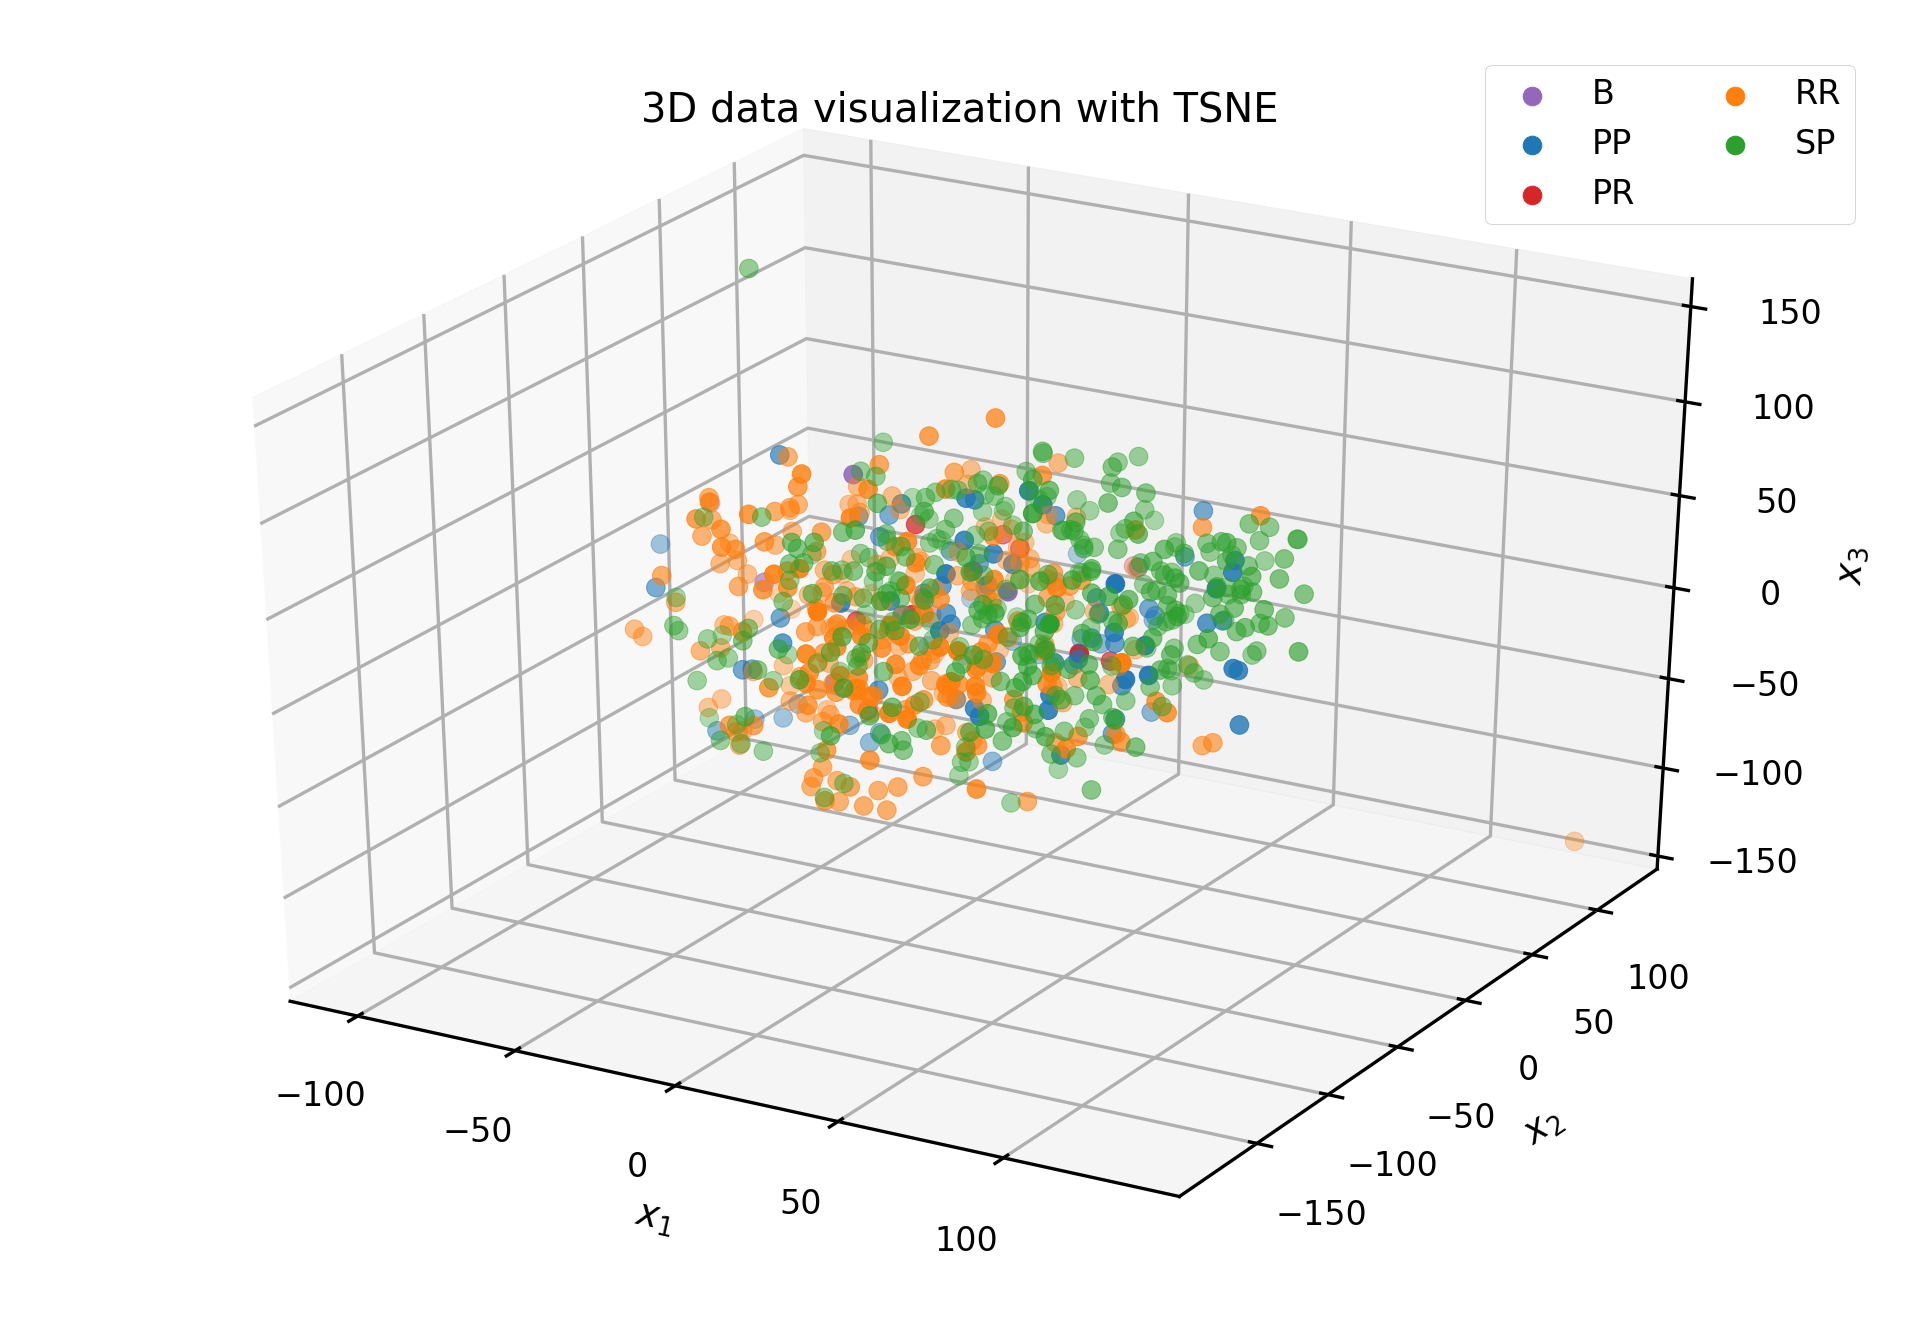
\includegraphics[width=0.5\textwidth]{part2/ms_tsne.png}
%		\label{fig:ms_ms_tsne}%
%	}
	\caption{A random extraction of the $20\%$ of the MS dataset projected on a 3D space by linear PCA, panel (a), and Isomap, panel (b).} \label{fig:ms_3dscatterplot}
\end{figure}

This EDA raised our hopes to successfully perform a further supervised MS course classification and evolution prediction.

% The number of considered samples across examinations is hence $2699$, of which $1220$ \RR and $1579$ \SP.


\section{Supervised analysis}\label{sec:problem_description}

% We adopted suitable categorical data encoding and missing values imputing strategies to cope with these issues (see Section~\ref{sec:problem_description}).

%a machine-learning based temporal model that, extracting information from \PCOs data, is able to answer to
Predicting the MS course evolution can be split in three different related tasks: \f (\F), \g (\G) and \fog (\FOG).

\begin{enumerate}
	\item[] \textbf{\F} Given the $165$-dimensional representation of a patient at a fixed time point $\bm{x}_i^t$, this task consists in assigning the corresponding disease course $y_i^t$. \F can be translated into a binary classification problem and which can be solved by learning a discriminative function $f(\bm{x}_i^{t}) = y_i^{t}$.
	
	\item[] \textbf{\G} Given the historical representation  of a patient $\bm{x}_i^t$ for $t=1,\dots,\tau$, this task consists in predicting the patient representation $\bm{x}_i^{\tau+1}$. \G can be seen as a multiple-output regression function and it can be solved by learning an appropriate function $g(\bm{x}_i^{t}) = \bm{x}_i^{t+1}$.
	
	\item[] \textbf{\FOG} This task can be seen as foreseeing the MS disease course $y_i^{\tau+1}$ from $\bm{x}_i^t$ for $t=1,\dots,\tau$. Once $\hat{f}(\bm{x})$ and $\hat{g}(\bm{x})$ are learned by training on historical \PCO data, the \FOG problem is finally solved by the temporal model $\hat{f} \circ \hat{g}(\bm{x}_i^{t}) = y_i^{t+1}$. In time-series data analysis, this is known as \textit{one-step-ahead forecast}. Notably, the \FOG model allows to foresee if the patient at the next time point is going to experience a transition from \RR to \SP, or not.

\end{enumerate}

All these predictive models assume the temporal structure outlined in Figure~\ref{fig:pipeline}.

% documentclass[letter,10pt]{article}
% \usepackage{amsmath}
% \begin{document}

\begin{figure}[]
  \centering
  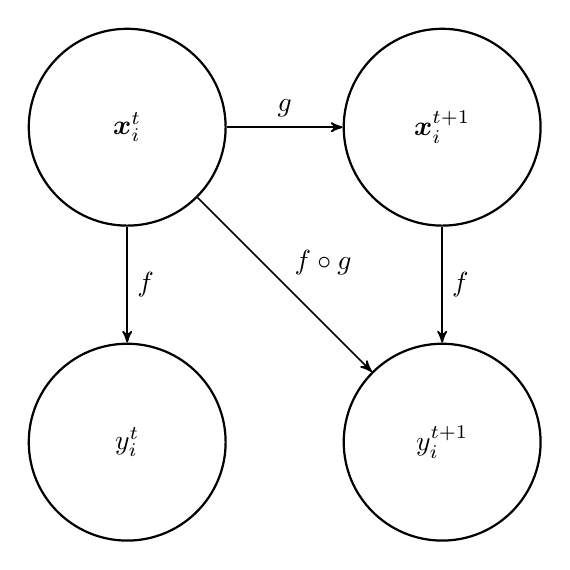
\begin{tikzpicture}[->, >=stealth', auto, semithick, node distance=4cm]
    \tikzstyle{every state}=[fill=white,draw=black,thick,text=black,scale=1, minimum height=2.5cm]
    \node[state]    (xit)                     {$\bm{x}_i^t$};
    \node[state]    (yit)[below of=xit]       {$y_i^t$};
    \node[state]    (xit1)[right of=xit]      {$\bm{x}_i^{t+1}$};
    \node[state]    (yit1)[below of=xit1]     {$y_i^{t+1}$};
    \path
    (xit)  edge node{$f$} (yit)
    (xit)  edge node{$g$} (xit1)
    (xit1) edge node{$f$} (yit1)
    (xit)  edge node{$f\circ g$} (yit1);
  \end{tikzpicture}
  \caption{A visual representation of the temporal structure assumed in the collected data. When the two functions $f$ (\F) and $g$ (\G) are learned, the \FOG model $f\circ g$ is able to predict the evolution of the disease course for future time points $y_i^{t+1}$.}\label{fig:pipeline}
\end{figure}
% \end{document}



\subsection{Experimental design}\label{sec:experimental_design}
Our final goal is predicting MS course evolution of  \RR and  \SP patients, hence the subjects with \PR, \PP and benign forms are not further taken into account.

We considered all the patients with a minimum of $1$ time point (the most recently enrolled) up to $T=11$ time points for a total of $3398$ samples, of which $1451$ \RR and $1947$ \SP. As this is an ongoing project, the number of PwMS decreases with time.
%We expect to fill the gap of samples between \textit{Exam~$1$} and \textit{Exam~$11$} by the end of the funded study.

Following the EDA, we opted for a preliminary feature-wise min-max scaling.
However, to promote unbiasedness on the results, this preprocessing phase is not performed on the entire data collection, but it is embedded into the model fitting procedure.
%separately evaluated prior to each model fitting process on its training cross-validation portion of the data.


We shall discuss separately the experimental designs used to learn $f(\bm{x})$ and $g(\bm{x})$.

% In particular, the training set comprises all samples collected at time points $t = 1, \dots ,T_{tr}$, the validation set at $t=T_{tr}+1,\dots,T_{vld}$ and the test set at $t=T_{vld}+1,\dots,T$.
% Here, as the maximum number of collected time points is $T=8$, we fixed $T_{tr} = 3$ and $T_{vld} = 4$.
% In particular, the training set comprises all samples collected at time points $t = 1, \dots ,T_{tr}$, the validation set at $t=T_{tr}+1,\dots,T_{vld}$ and the test set at $t=T_{vld}+1,\dots,T$.

\begin{itemize}
	\item[] \textbf{\F} The \F model $f(\bm{x})$ solves a binary classification problem: to each input $\bm{x}_i^t$ is associated  an output $y_i^t$ that encodes the corresponding MS disease course (\RR or \SP) with a binary label.
	We split the dataset in three temporal chunks, namely \textit{training}, \textit{validation} and \textit{test} sets, consisting of all samples collected at time points $t=1,2,3$, $t=4$ and $t=5,6,7,8,9,10,11$, respectively.
	Accordingly, we used $1993$ samples for training $f(\bm{x})$, $463$ for validation leaving the remaining $942$ for test.
	
	Five candidate models for $f(\bm{x})$ are fitted on $100$ Monte Carlo (MC) random sampling of the training set each time keeping $\frac{1}{4}$ of the samples aside~\cite{molinaro2005prediction}. For each MC sampling the fitting procedure is performed on the remaining $\frac{3}{4}$ of the samples and it includes an inner parameter optimization via grid-search cross-validation~\cite{hastie2009elements}. In particular, we require the MS course prediction to be based on a reduced number of variables (see Section~\ref{sec:learning_f}), therefore we enforce sparsity in each candidate model.
	% Each candidate model is required to be sparse, therefore the MS course prediction is based on a reduced number of variables (see Section~\ref{sec:learning_f}).
	Leveraging on the MC strategy, we rank the variables according to their selection frequency~\cite{barbieri16palladio, meinshausen2010stability}.
	Once a variable ranking is achieved for each candidate model, the list of selected variables is identified by thresholding the corresponding ranking with the threshold that maximizes the accuracy \todo{or MCC} on the validation set. Finally, the last training step consists in fitting each candidate model on the union of training and validation sets taking only into account the corresponding reduced subset of selected variables. The final \F model $\hat{f}(\bm{x})$ is chosen as the one that performs better on the previously unseen test set in terms of accuracy, \todo{MCC}, precision, recall and $\text{F}_1$ score.

	\item[] \textbf{\G} %presents the answers provided by the MS patients to the \PCOs questionnaires, while the label vector $\bm{y}$ has the corresponding disease form diagnosis.
	On the other hand, learning the \G model $g(\bm{x})$ implies solving a multiple-output regression problem and each input $\bm{x}_i^t$ is associated with the output vector $\bm{x}_i^{t+1}$.
	% and the class labels are not taken into account.
	Therefore, we can only consider samples at time point $t$ with an available follow-up at the next time point $t+1$, which reduces the overall number of available samples.
	The dataset splitting is consistent with the one followed for learning $f(\bm{x})$, although there is no need for a separate validation set, as learning $g(\bm{x})$ does not require any variable selection process. We used the samples collected at time points $t=1,2,3$ for training and those at $t=4,5,6,7,8,9,10,11$ for test, resulting in $XXXX$ and $XXX$ samples, respectively.
	The fitting procedure includes an inner parameter optimization via grid-search cross-validation. Each candidate model is a function
	$g: \mathbb{R}^{165} \rightarrow \mathbb{R}^k$ where $k$ is the number of variables selected by the best \F model.
	% that predicts the evolution of the variables selected by the best \F model starting from the full set of \PCOs.
	The final \G model $\hat{g}(\bm{x})$ is chosen as the candidate model that performs better on the previously unseen test set in terms of mean absolute error (MAE).
	

	\item[] \textbf{\FOG} The predictive capability of the \FOG model $\hat{f} \circ \hat{g}(\bm{x})$ is finally evaluated on the test set. The \F model $\hat{f}(\bm{x}_i^t)$ predicts the MS course $\hat{y}_i^t$ from the \PCO data vector $\hat{\bm{x}}_i^t$ that, in turn, is predicted by the \G model $\hat{g}(\bm{x}_i^{t-1})$. We shall notice here that the predictions $\hat{f} \circ \hat{g}(\bm{x}_i^t)=y_i^{t+1}$ for $t=11$ are foreseeing possible \RR to \SP transitions that are beyond our data observation, hence predictions at the last time point cannot be used to assess the \FOG model performance. Therefore, its performance is evaluated only on $XXXX$ test samples.
	
\end{itemize}




%Finally, the predictive capability of the prognosis model $\hat{f} \circ \hat{g}(\bm{x})$ is evaluated by predicting $\hat{g}(X_{T-1})=\hat{X}_T$, that is the evolution of the \PCOs for the patients at time point $T-1$, then applying the diagnosis model on the predicted data matrix $\hat{f}(\hat{X}_T)=\hat{y}_T$ and comparing them with the diagnosis provided by the doctors at the same examination.



\subsection{Learning $f(x)$} \label{sec:learning_f}


%First, we will require the diagnosis function $f(\bm{x})$ to be sparse, hence the MS outcome prediction will be based on a reduced number of variables.
We imposed $f(\bm{x})$ to be sparse. This requirement is helpful from two distinct respects:
\begin{enumerate*}[label=\alph*)]
	\item the performance of the predictive model may increase thanks to a reduced effect the course of dimensionality~\cite{hastie2015statistical} and
	% \item the effect the course of dimensionality~\cite{hastie2015statistical} may be attenuated, hence increasing the performance of the predictive model, and
	\item the identification of a reduced subset of meaningful \PCOs provides interpretability of the results for the clinicians.
\end{enumerate*}
In order to achieve such sparse model, we take advantage of two main variable selection strategies: embedded and wrapper methods~\cite{guyon2003introduction}.
When using embedded methods, we exploited the sparsity inducing penalties of EN to take into account possible correlation between \PCO variables and of SLR to benefit from the renowned classification capability of the logistic loss function.
We applied the RFE wrapper method to
% Concerning the use of wrapper methods, which exploit a RFE schema, we chose
two tree-based learning machines (RF and GB) that are capable of capturing nonlinear relationship between input and output and are intrinsically well-suited to deal with categorical/ordinal variables. We also explored the use of RFE with SVM, as in~\cite{guyon2002gene}.
% which is a state-of-the-art machine learning method for classification.

\subsection{Learning $g(x)$}

As no prior information on the relationship between \PCOs evaluated at different time points was available, to learn $g(\bm{x})$ we investigated on the use of both linear and nonlinear models.
% To learn $g(\bm{x})$ no prior information on the relationship between \PCOs evaluated at different time points was available. To achieve our goal, we investigated on the use of both linear and nonlinear models.

Concerning the linear models, we explored two different solutions: NNM and MTEN. The first imposes a low-rank prior on the result. The second is a natural multiple-output extension of EN, hence it induces a row-structured sparsity pattern on the solution where collinear variables are more likely to be included in the model together. For nonlinear prediction, we resorted to the state-of-the-art MLP approach.

\section{Results}\label{sec:results}

% \todo{add table of selected features}
We shall discuss separately the results achieved in terms of \F, \G and \FOG models.

Regarding \F, the GB method outperforms the other candidate models reaching accuracy $0.900$, precision $0.936$, recall $0.899$ and $\text{F}_1$ score $0.917$, as shown in Figure~\ref{fig:diagnosis_competition}. Therefore we chose it as \F model $\hat{f}(\bm{x})$.
Insights on the use of \PCOs for MS assessment are provided by the sparsity of the \F model induced by the RFE schema.
The $31$ selected variables are reported in Table~\ref{tab:selected}.
Comparing the full list of \PCO questionnaires of Table~\ref{tab:proms} with Table~\ref{tab:selected}, we observe that each \PCO used in this study is represented at least once, except \EDINB, and the most represented is \FIM.
We also see that, whenever possible, the model tends to select aggregate scores (total and subtotal) rather that single items. This is consistent with the clinical practice, where neurologists are more likely to assess patient's health status by using the aggregate scores, rather than the single questions.
Quite surprisingly, the recent number of relapses is the only additional information not selected by the model.
Finally, we note that all the domains that are known to be affected by the disease are well covered: mobility (upper and lower limbs), cognition, emotional, fatigue, bladder and psychosocial.
The heatmap in Figure~\ref{fig:selection_heatmap} shows the Hamming distance estimated across the list of variables selected by the five \F candidate models. Interestingly, tree-based methods are more prone to select similar variables with respect to linear methods. As expected, the sparsity induced by the $\ell_1$-norm of SLR allows the method to achieve a list of variables similar to the one obtained by SVM-RFE, while the list obtained by ENET includes collinear variables and it is significantly different from the others.

Regarding \G, MTEN outperforms the other candidate models in terms of MAE ( $\text{MAE}_{\text{MTEN}}=0.095$, $\text{MAE}_{\text{NNM}}=0.102$, $\text{MAE}_{\text{MLP}}=0.105$), hence we select it as our \G model $\hat{g}(\bm{x})$.


 \begin{figure}[h!]
	\centering
	\subfloat[]{%
		\includegraphics[width=0.5\textwidth]{part2/final_scores_2_copy.png}
		\label{fig:diagnosis_competition}%
	}%
	 \hfill%
	\subfloat[]{%
		\includegraphics[width=0.5\textwidth]{part2/selection_heatmap_copy.png} \label{fig:selection_heatmap}
	}%
	\caption{A visual representation of the results obtained from the \F model. On the left panel (a) we show the classification performance achieved on the test set by the candidate models. Precision, recall and $\text{F}_1$ score are estimated considering \SP as the positive class. As GB outperforms the other methods on each performance metric, it is chosen as \F model. On the right panel (b) a heatmap displays the distance between the lists of variables selected by each model in terms of their hamming distance. \todo{break figure in two}}\label{fig:f}
\end{figure}


%
Finally, the \FOG model $\hat{f} \circ \hat{g}(\bm{x})$, obtained by combining MTEN and GB achieves the following performance scores on the $220$ test samples: accuracy $0.841$, precision $0.900$, recall $0.824$ and $\text{F}_1$ score $0.860$.


\section{Conclusions and future works}

This chapter describes a temporal model based on \PCOs and ML for disease form prediction in MS.
In particular, we address the tasks of current course assignment, \PCOs evolution prediction and future course assignment. The model is built on a collection of \PCOs acquired on a cohort of individuals enrolled in an ongoing funded study (\textit{DETECT-MS PRO}).

% The measures are categorical or ordinal answers to a given set of \PCOs.
\PCOs data are typically used to corroborate evidence provided by quantitative exams, in our case the absence of clear MS disease form predictors makes the information extracted from \PCOs data the only available resource.
The proposed temporal model was able to correctly assign the current MS form and to foresee future ones with accuracy of $90.0\%$ and $84.1\%$, respectively \todo{fixme}.
This demonstrates that \PCOs can effectively be used as MS disease course predictor.
%In the next future, we plan to expand the data collection with respect to the amount of enrolled subjects as well as the number of time points.

In the next future, we plan to further investigate on the predictive capabilities of the proposed model with longer temporal horizons and to compare it with different approaches, such as probabilistic graphical models.
%, that allow to explicitly incorporate the temporal nature of the data.}

Given the achieved promising results, the proposed model is soon going to be validated in clinical practice, where it will assist the clinicians involved in this study to foresee possible disease course transition and to take important decisions concerning treatment and therapies that can substantially improve the quality of life of their patients.
% In fact, the proposed temporal model was able to correctly foresee the evolution of the disease form of $84.1\%$ of MS patients.

In the context of neurodegenerative diseases, clinicians typically use \PCOs data to corroborate evidences coming from standard quantitative exams \cite{black2013patient}. Interestingly, in our case the absence of clear \SP predictors makes the information extracted from \PCOs data the only available resource.
%Our result shows that a timely prediction of the disease course can be obtained from patient-friendly and low-cost measures.

In the era of precision medicine, the problem of predicting MS course evolution still relies on stressful exams and clinical judgement.
To the best of our knowledge, this is the first attempt to solve this delicate task leveraging only on patient-friendly measures and ML.



% !TEX root = ../main.tex

\chapter{Data-driven strategies for robust forecast of continuous glucose monitoring time-series} \label{chap:diabete}
% EMBC

\begin{displayquote}
\textit{Over the past decade, continuous glucose monitoring (CGM) has proven to be a very resourceful tool for diabetes management. To date, CGM devices are employed for both retrospective and online applications. Their use allows to better describe the patients' pathology as well as to achieve a better control  of  patients' level of glycemia. The analysis of CGM sensor data makes possible to observe a wide range of metrics, such as the glycemic variability during the day or the amount of time spent below or above certain glycemic thresholds. However, due to the high variability of the glycemic signals among sensors and individuals, CGM data analysis is a non-trivial task. Standard signal filtering solutions fall short when an appropriate model personalization is not applied. State of the art data-driven strategies for online CGM forecasting rely upon the use of recursive filters. Each time a new sample is collected, such models need to adjust their parameters in order to predict the next glycemic level. In this chapter we will see that the problem of online CGM forecasting can be successfully tackled by personalized machine learning models, that do not need to recursively update their parameters.}
\end{displayquote}

\section{Introduction: modern diabetes care}
Diabetes is a chronic metabolic disorder affecting nearly $400$ million of individuals worldwide. The number of diabetic patients is increasing and it is expected to reach almost $600$ million in the next future~\cite{guariguata2014global}.
%In the world people with type 2 diabetes are $400$ million and this  number will rise to $600$ million in $2035$~\cite{guariguata2014global}. 
%http://www.who.int/diabetes/global-report/en/
%https://www.cdc.gov/diabetes/statistics/incidence/fig2.htm
According to the {\em World Health Organization}~\cite{world2016global}, the global prevalence of diabetes among adults has nearly doubled in the last few decades, rising from $4.7\%$ in 1980 to $8.5\%$ in 2014.
%and its incidence per year is $6.9$ per $1,000$ individuals~\cite{}.
%In the western population the  prevalence of diabetes is $6$ to $10\%$ .
%The incidence of diabetes type $2$ is $5-7/1000/$year \todo{non sono sicuro di aver capito}.
If not treated correctly, diabetes may cause several permanent complications, such as visual impairment and kidney failure. 
%, that heavily affect the quality of life of the patients

Hypoglycemia is a severe risk in diabetes therapy. 
The mean incidence of hypoglycemia in patients with type $1$ diabetes (T1D) 
is 1-2 events per week, while severe hypoglicemia occurs 0.1-1.5 episodes per year~\cite{van2016continuous}. 
Moreover, hypoglycemia interferes with the quality of life and increases the risks of cardiovascular events in type $2$ diabetes (T2D) patients~\cite{van2016continuous}. On the other hand, hyperglycemia associates with an increased risk of diabetes complication as well.


The most common glucose monitoring solutions are self blood glucose meters and Continuous Glucose Monitoring systems (\ac{CGM}). 
CGM devices are minimally-invasive, and can be used in daily life for retrospective or online applications~\cite{vigersky2017role}. 
CGM systems measure interstitial glucose concentration at fixed time intervals, enabling an accurate observation of glycemic variability during the day as well as the ratio of time spent in hypo/hyperglycemia. 
When CGM is employed online, an improvement of the therapy can be achieved by embedding in the system a tool that foresees glucose levels using suitable time-series models trained on past  CGM  data~\cite{sparacino2007glucose}. In this case, alarms can be generated when the glucose concentration exceeds the normal range~\cite{vigersky2017role}.
%thresholds

%Such tools implement algorithms to foresee hypo/hyperglycemic  events that can be obtained  by  generating alerts on  the basis of future glucose level forecast by  using  past  CGM  data  and  suitable time-series  models \cite{sparacino2007glucose}.
%\cite{monnier2016near}
%\todo{
%State-of-the-art in diabetes monitoring is glycemia self assessment via glucose meters~\cite{monnier2016near} NON SONO SICURO DELLA REF},   it is possible to self-manage diabetes with continuous glucose monitoring (CGM) devices. CGM systems measure interstitial glucose concentration at fixed time intervals (e.g., each $5$ minutes). 
%
%CGM enables the observation of glycemic variability during the day as well as the ratio of time spent in hypo/hyperglycemia. 
%
%
%These devices are minimally-invasive, and can be used in daily life, but, to date, they are mainly used for retrospective and online applications~\cite{vigersky2017role}. 
%
%In both cases, CGM enables the observation of glycemic variability during the day as well as the ratio of time spent in hypo/hyperglycemia. 
%
%When CGM is employed online, an improvement of the therapy can be achieved by embedding in the system a tool able to generate alerts when the glucose concentration exceeds the normal range thresholds~\cite{vigersky2017role}, based on past  CGM  data  and  suitable time-series  models \cite{sparacino2007glucose}.

%In many clinical situations


To model patient-specific Blood Glucose (BG) levels, several approaches, integrating various information, were proposed~\cite{bunescu2013blood, zecchin2011new}. However, the problem of glycemic level prediction is still challenging, due to the high CGM signal variability among patients and acquisition devices.

This chapter describes the third, and last, biomedical data science challenge of the thesis. Throughout this chapter we assume that CGM signals have structural information on time-changes of BG concentration \cite{sparacino2007glucose, bunescu2013blood} and we perform glycemic level forecasting exploring the performance of a set of purely data-driven techniques for time-series analysis.

Data-driven forecasting approaches, as opposed to models driven by an \textit{a-priori} description of the underlying phenomena, are capable of modeling input/output relationships without requiring prior knowledge on the field of use. This family of approaches can be successfully employed to obtain reliable predictions without modeling complex, and possibly not completely understood, environments. Data-driven forecasting models are widely applied in  real-world scenarios often employing a moving-window paradigm, \ie the system keeps track of the last $w$ acquisitions using them to forecast future values.

In this chapter, we focus on two main groups of data-driven methods for online time-series forecasting: \textit{recursive filters} and, of course, ML models.
The first group includes linear stationary models, such as Autoregressive Moving Average (\ac{ARMA}), non stationary models, such as Autoregressive Integrated Moving Average (\ac{ARIMA}) and adaptive filtering techniques, such as the Kalman Filter (\ac{KF}). These methods are well-established and extensively used, but they require recursive parameters adjustment for every new collected sample \cite{box2015time}.
As these methods are note covered in Chapter~\ref{chap:state-of-the-art}, a quick overview is provided in Section~\ref{sec:recursive_filters}. 

The second group comprises regularized kernel methods, such as Kernel Ridge Regression (\ac{KRR}) (see Sections~\ref{sec:ridge_regression} and~\ref{sec:kernel_trick}) and deep learning methods, such as Long Short-Term Memory networks (\ac{LSTM}), see Section~\ref{sec:lstm}.

As we have seen in the previous chapters, ML methods showed very promising results in several applications, also including time-series forecasting \cite{bunescu2013blood, schmidhuber2005evolino}. To achieve a predictive model, they need to learn the model parameters from a training set. This learning process is done \textit{only once} and it conveys a model that does not require further parameter adjustments to predict future values. This remarkable advantage makes machine learning models more suitable to be delivered on embedded portable systems.

This chapter aims at understanding whether purely data-driven machine learning methods can be successfully employed to forecast glucose values of diabetic patients.  

\section{Temporal forecasting problem setting}

%\todo{aggiustare il tiro qui}
%In this study we aim at comparing four different data-driven models
% for online CGM sensor data {\em forecasting}: {\em Auto Regressive Integrated Moving Average} (ARIMA) , {\em Kalman Filter} (KF), {\em Kernel Ridge Regression} (KRR) and {\em Long Short-Term Memory} (LSTM) {\em Network}.
In the previous chapters we fixed the notation for regression and classification problems. The temporal forecasting can be seen as a special regression case, therefore some additional notation is needed.

Given a set of data $\mathcal{S}$, we refer to data-driven models with hyperparameters $\bm{\theta}$ as $\mathcal{M}_\mathcal{S}(\bm{\theta})$.
%Given $y_i(t)$, the time-series associated with the $i$-th subject, for $t=t_k,\dots,t_{k+w}$ we aim at predicting $y_i(t_{k+w}+\Delta T)$, where $\Delta T$ is some prediction horizon.
Given the time-series $y(t)$ we aim at predicting $y(t+\Delta T)$, where $\Delta T$ is some {\em prediction~horizon}.

A well-known issue of CGM sensor data analysis is that signal properties, such as the signal-to-noise ratio, may vary among devices and individuals~\cite{facchinetti2010online}. In order to achieve an accurate forecast of the glucose level of a given individual from past samples, any prediction model $\mathcal{M}_\mathcal{S}(\bm{\theta})$ must be \textit{personalized}. Such model personalization procedure is two-fold: \textit{hyperparameters }($\bm{\theta}$) \textit{optimization}, also known as model selection (see Section~\ref{subsec:model_selection}), and {\em parameter estimation}, or model fitting. 
In this work we fixed a common strategy for hyperparameters optimization whilst the actual model fitting procedure is defined differently according to the model. 
%(i.e., $25$ hours at 5 minutes sampling period)(in our dataset, this set lasted up to $6$ days)

\section{Recursive filters overview} \label{sec:recursive_filters}
Recursive filters are the most widely adopted class of temporal forecasting strategies.
In this chapter we make CGM temporal prediction by exploiting two different recursive filters approaches: ARIMA and KF. Providing a comprehensive overview of temporal forecasting strategies is beyond the scope of this thesis, therefore Chapter~\ref{chap:state-of-the-art} does not cover this topic. This section sketches the main ideas behind this two strategies, providing the information that are necessary to understand this last biomedical data science challenge.

\subsection{Autoregressive Integrated Moving Average}
ARIMA methods can be used to perform linear forecasting of non stationary time-series assuming that its $d$-th difference is a stationary ARMA process  \cite{box2015time}. The output of an ARMA process, with white input noise $u(t)\sim\mathcal{N}(0,\sigma^2)$, can be expressed as in Equation~\eqref{eq:arma}.
\begin{equation} \label{eq:arma}
y(t) = -\sum_{k=1}^pa_ky(t-k)+\sum_{k=0}^qb_ku(t-k)
\end{equation}
The output of an ARMA$(p, q)$ model can be seen as the sum of $p$ autoregressive and $q$ moving average terms. This strategy requires the modeled processes to be stationary. On the other hand, when a time-series can be considered stationary after $d$ differentiations, ARIMA$(p, d, q)$ models can be used. 
This is the case for non stationary time-series that exhibit local stationary behavior. In general,  $(p, d, q)$ are unknown and we will consider them as hyperparameters of the ARIMA model.

The cross-validation index (see Section~\ref{sec:diabete_expdesign}) for ARIMA models can be defined as $J(\bm{\theta})= \text{AIC}(\mathcal{M}_{\mathcal{S}}(\bm{\theta})) + \bar{\varepsilon}_{\text{cv}}$, where AIC stands for Akaike Information Criterion~ \cite{box2015time} and $\bar{\varepsilon}_{\text{cv}}$ is the MSE evaluated via cross-validation, see Section~\ref{sec:performance_metrics}. We refer to~\cite{box2015time} for a detailed description of ARIMA model fitting.

The application of this class of models to predict CGM sensor data was also explored in \cite{sparacino2007glucose,bunescu2013blood}.

\subsection{Kalman Filter}
%\begin{equation}\label{eq:kfx}
%x(t+1) = Fx(t) + w(t)
%\end{equation}
%with measurements $y \in \mathbb{R}^k$,
%\begin{equation}\label{eq:kfy}
%y(t) = Hx(t)+v(t)
%\end{equation}


The KF addresses the problem of estimating the state $\bm{x} \in \mathbb{R}^d$ of a discrete-time process governed by the linear stochastic difference equation
$\bm{x}(t+1) = F\bm{x}(t) + \bm{w}(t)$
with measurements $\bm{y} \in \mathbb{R}^k$,
$\bm{y}(t) = H\bm{x}(t)+\bm{v}(t)$,
where $\bm{w}(t)$ and $\bm{v}(t)$ are independent random variables representing state and measurement noise, respectively \cite{welch1995introduction}. It is usually assumed that $\bm{w}(t)\sim \mathcal{N}(\bm{0}, Q)$ and $\bm{v}(t)\sim \mathcal{N}(\bm{0}, R)$, with both $Q$ and $R$ unknown. In the context of CGM sensor data prediction, we can safely assume that the state space is two-dimensional, hence $x_1(t)=u(t)$, $x_2(t)=u(t-1)$ where the unknown signal $u(t)$ is described {\em a-priori} as an integrated random-walk $u(t)=2u(t-1)-u(t-2)+w(t)$ as in \cite{facchinetti2010online}. Consequently, the state space transition matrix $F$ can be written as
%$$F=[\begin{smallmatrix}  2 & -1  \\  1 & 0\end{smallmatrix}]$,
\begin{equation}\label{eq:F}
F=
\begin{bmatrix}
2 & -1  \\
1 & 0
\end{bmatrix}
\end{equation}
while the measurement vector is
$$
H =
\begin{bmatrix} 1 & 0
\end{bmatrix}
$$
the process noise covariance is
%$Q=
%[\begin{smallmatrix}
%\lambda^2 & 0  \\
%0 & 0
%\end{smallmatrix}
%]$
\begin{equation}\label{eq:Q}
Q=
\begin{bmatrix}
\lambda^2 & 0  \\
0 & 0
\end{bmatrix}
\end{equation}
and the measurement noise covariance is $R = \sigma^2$, as in \cite{facchinetti2010online}. Both $\lambda^2$ and $\sigma^2$ are unknown and we will consider them as hyperparameters of the KF forecasting strategy.

In this case, the cross-validation index (see Section~\ref{sec:diabete_expdesign}) can be defined as $J(\bm{\theta})= \bar{\varepsilon}_{\text{cv}}$.

The application of KF to predict CGM sensor data was also explored in \cite{facchinetti2010online, knobbe2005extended}.

\section{CGM data collection}
%{\color{red}We collected samples from 178 type 1 and type 2 diabetes patients were monitored for about 1 to 7 days in  free living conditions.
%Patients wore the iPro\textsuperscript{\footnotesize \textregistered}2 Professional CGM (Medtronic), which reported glucose values every 5 minutes}.\\
%

%Patients wore the iPro\textsuperscript{\footnotesize \textregistered}2 Professional CGM sensor (Medtronic), which reported glucose values every 5 minutes.

We acquired CGM samples from a group of 148 T1D and T2D patients wearing the iPro\textsuperscript{\footnotesize \textregistered}2 Professional CGM sensor (Medtronic), which reported glucose values every 5 minutes. Patients were monitored for up to 7 days in  free living conditions, keeping track of their treatments. %, as in Figure~\ref{fig:cgm}. 
From this initial cohort, we excluded the 18 individuals which acquisitions lasted for less than 3.5 days as well as the 24 time-series that presented artifacts due to incorrect use of the CGM acquisition device. Hence, our final dataset comprises 106 subjects of which 72 T1D and 34 T2D. 
On average, glycemic variability is relatively high, with $170.7\pm 70.0$ mg/dL for T1D and $158.4\pm 43.6$ mg/dL for T2D. Figure~\ref{fig:cgm} shows two examples, one for each diabetes type.
%For analysis purposes, patients having CGM acquisitions shorter than 3.5 days or presenting heavy artifacts were discarded.
%\subsection{Data Exploration}

\begin{figure}[]
	\caption{Plots reporting the distributions of LBGI (left) and HBGI (right) for T1D and T2D. Green areas at the bottom of each plot represents low risk of hypo/hyperglycemia events.
		%  LBGI values below 2.5 indicate a low risk of hypoglycemia, while values above 5 correspond to an 
		%  Normal range for LBGI is $2.5-5$ and for HBGI is $10-15$.
	}\label{fig:plots}
	\centering
	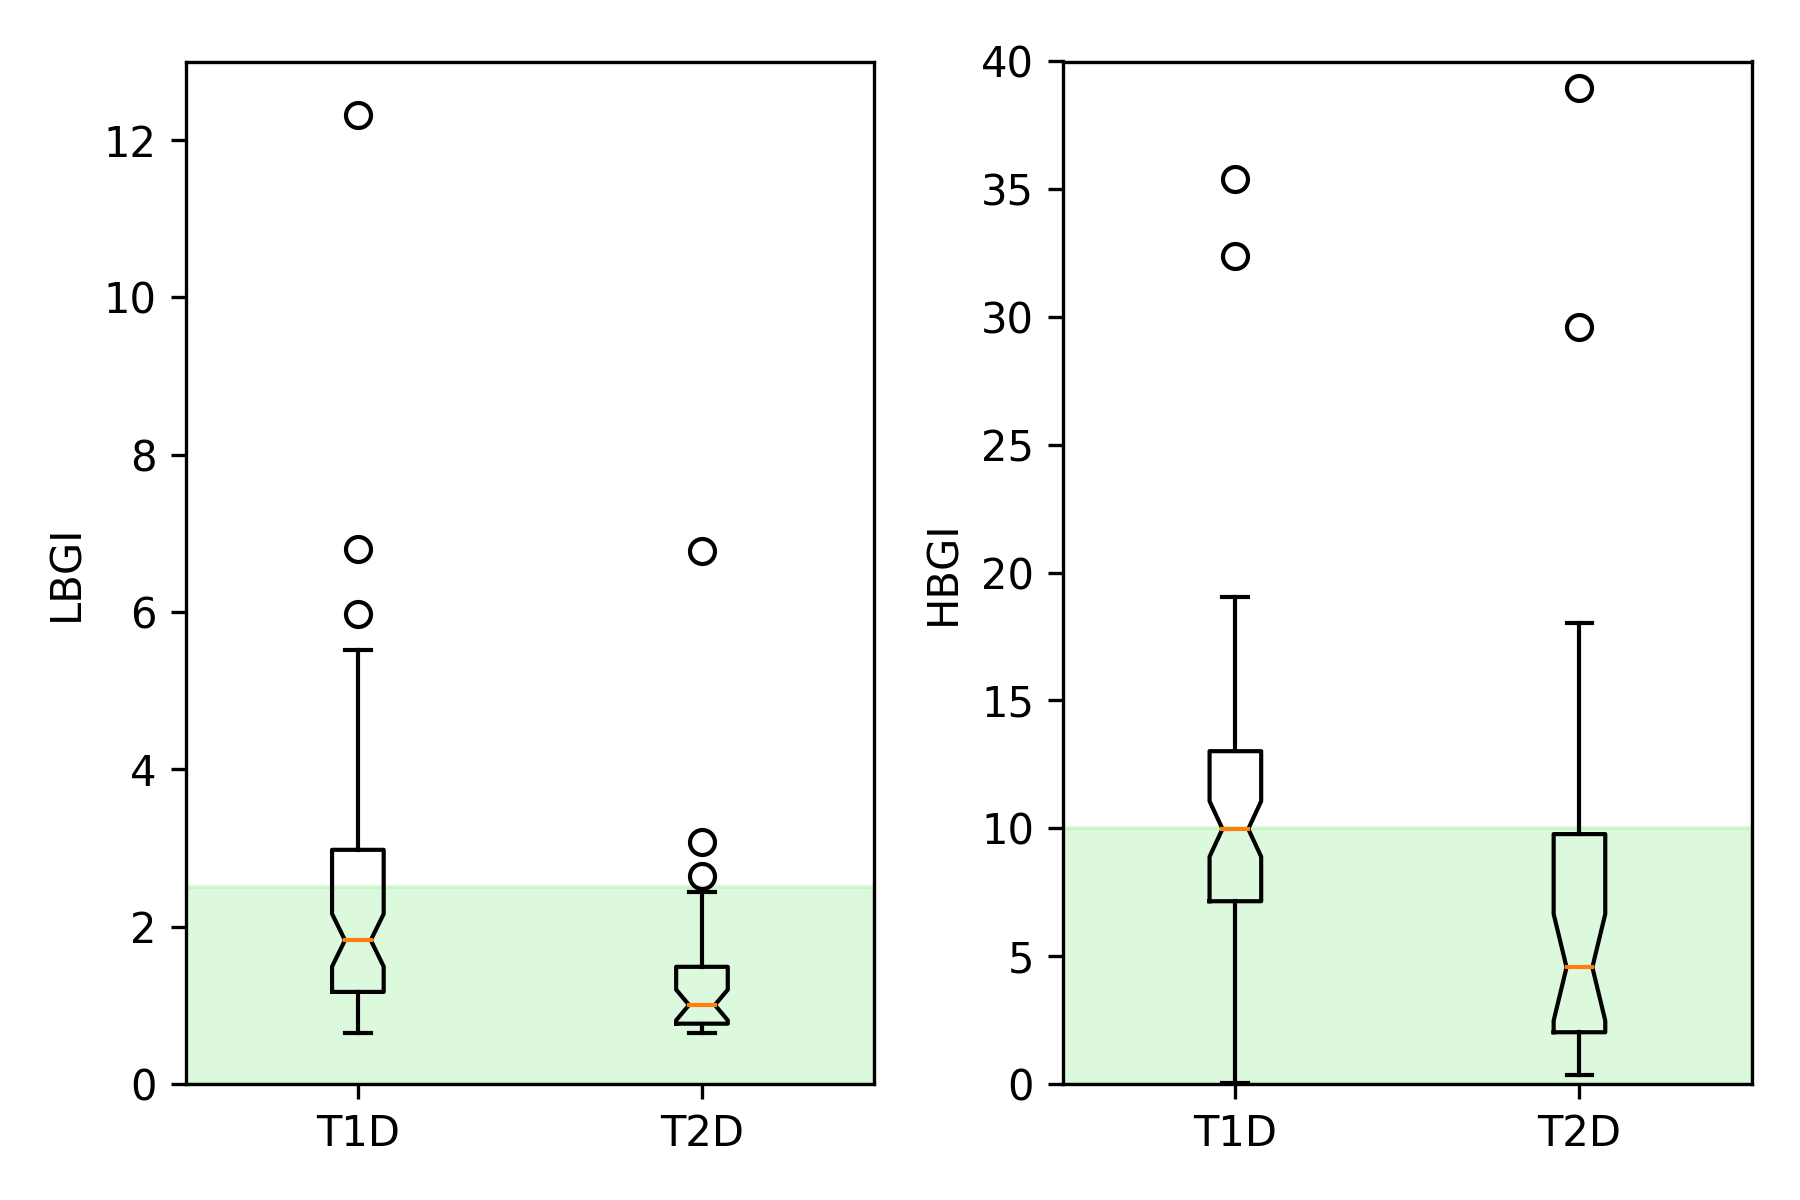
\includegraphics[width=0.8\textwidth]{part2/boxes.png}
\end{figure}

\section{CGM exploratory data analysis}
For each patient, the risk of hypo/hyperglycemia is determined by computing the Low Blood Glucose Index (\ac{LBGI}) and the High Blood Glucose Index (\ac{HBGI}), defined as in~\cite{fabris2016risk}.
LBGI and HBGI are summary statistics, extracted from a series of CGM data, that increases when the frequency and/or the extent of low CGM or high CGM readings increases.
These two indices are heavily influenced by the frequency and extent of hypo- and hyper-glycemic episodes.
To estimate LBGI and HBGI from CGM data we followed~\cite{kovatchev1997symmetrization}.
Figure \ref{fig:plots} shows the LBGI and HBGI distributions for T1D and T2D. The green areas at the bottom of each boxplot represents the low risk area for hypo/hyperglycaemia, as reported in literature~\cite{kovatchev1997symmetrization}.
As expected, the fraction of T1D patients experiencing risks of hyperglycaemia episodes is higher than T2D patients.


\begin{figure}
	\caption{An example of two glycemic profiles obtained from T1D and T2D patients. The glucose target range is set between $70$ mg/dL and $140$ mg/dL (dashed lines). The yellow area at the left hand side of the plot is the initial {\em burn-in} interval used for model {\em personalization}.}\label{fig:cgm}
	\centering
	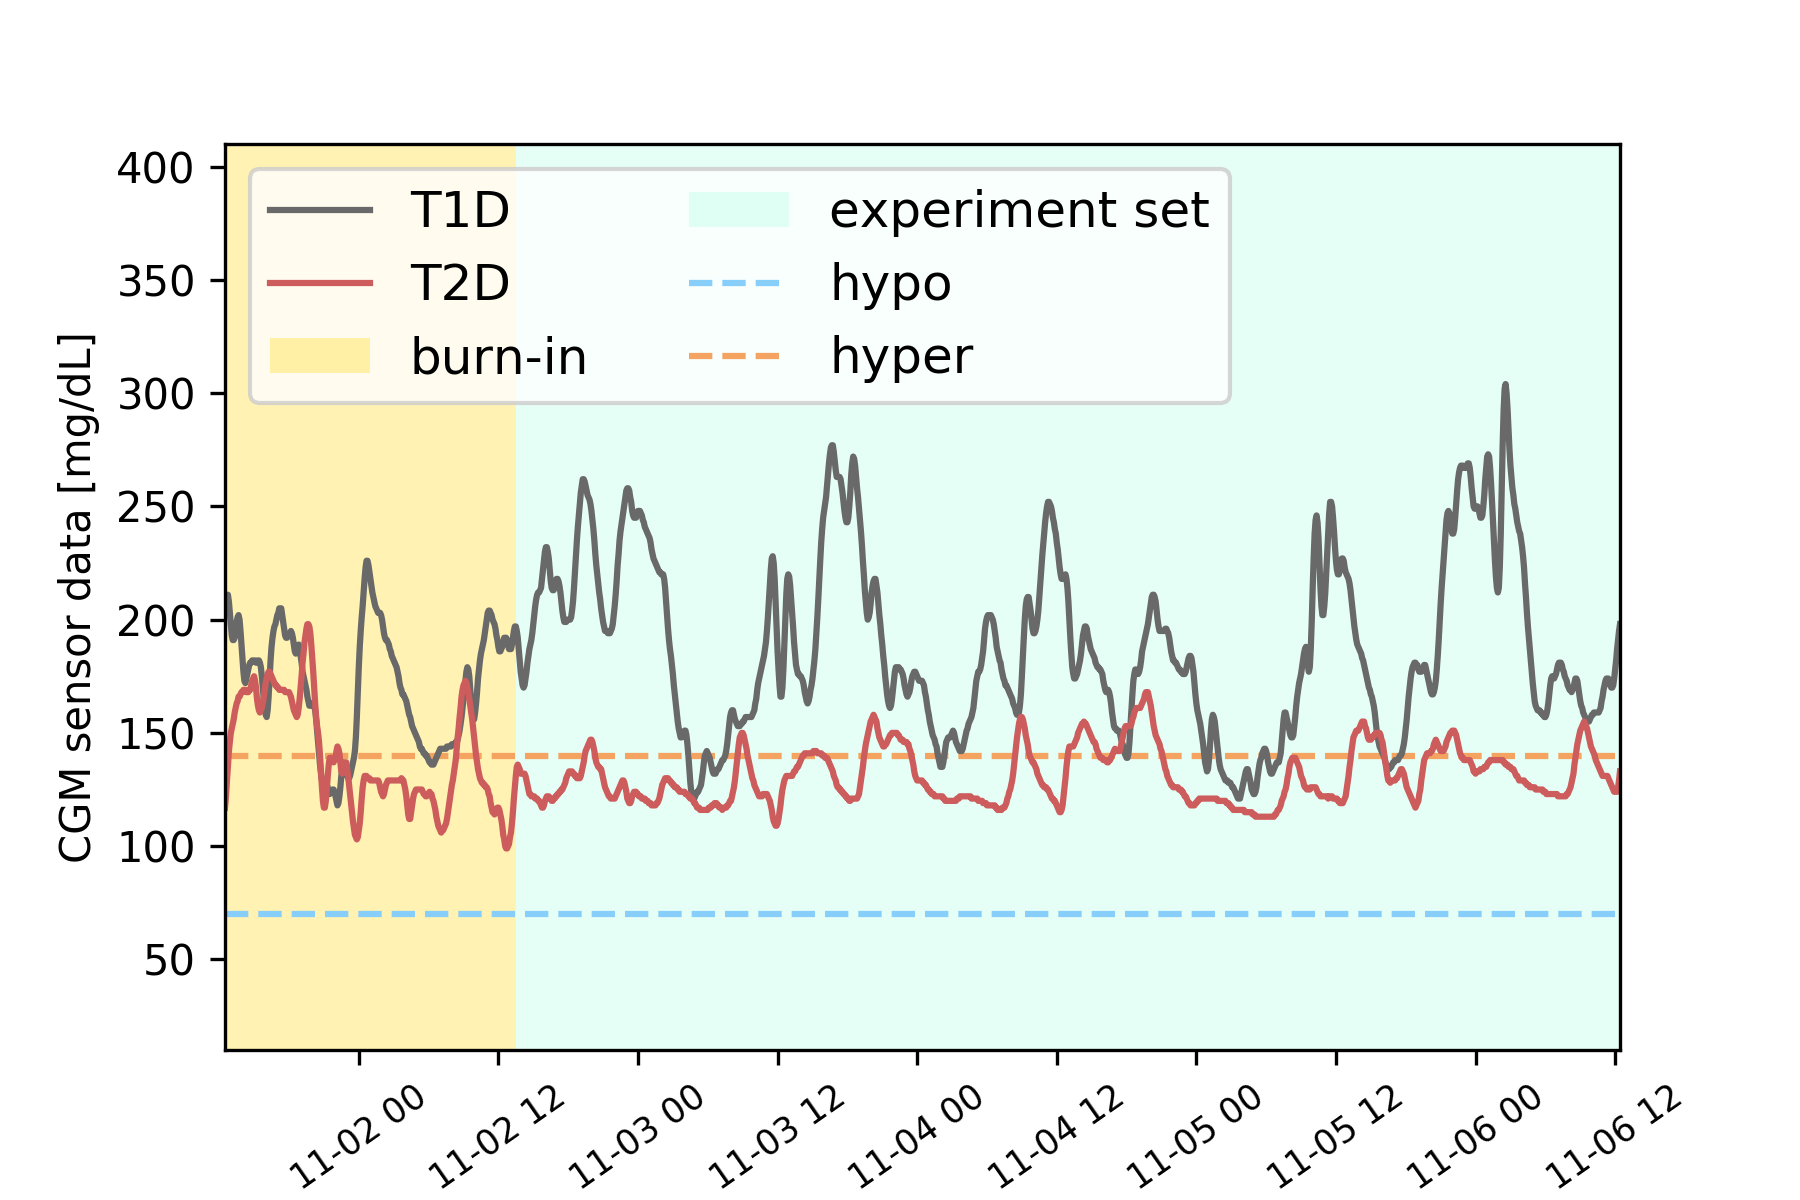
\includegraphics[width=0.8\textwidth]{part2/cgm_values.png}
\end{figure}

\section{Experimental design} \label{sec:diabete_expdesign}

We shall now focus on the hyperparameters optimization strategy.
Given $y(t)$ for time points $t=1,\dots,T$, we split the time-series in two chunks: an initial {\em burn-in} of $T' = 300$ CGM observations and the {\em experiment set} made of the subsequent $T - T'$ samples (see Figure~\ref{fig:cgm}). For each model $\mathcal{M}_\mathcal{S}(\bm{\theta})$, and for each subject, we use the burn-in samples to optimize the hyperparameters $\bm{\theta}$ via grid-search cross-validation. In other words, the best hyperparameters $\bm{\theta}^*$  are chosen as the ones that minimize an index $J(\bm{\theta})$ estimated on cross-validation splits and defined differently according to the model, as anticipated in the previous sections. %, hence $\bm{\theta}^* = \argmin{\bm{\theta}} J(\bm{\theta})$.

In the context of time-series, the cross-validation training splits consist only of observations occurred before the corresponding validation samples; such cross-validation flavor is sometimes referred to as {\em rolling forecasting origin}~\cite{tashman2000out}. The grid-search cross-validation scheme promotes the identification of models capable of returning robust predictions. %, where the negative influence of the variable SNR is reduced.

Once the best hyperparameters $\bm{\theta}^*$ are identified, the model $\mathcal{M}_\mathcal{S}(\bm{\theta}^*)$ is fitted on the whole burn-in and it is used to perform online forecasting on the data points of the experiment set (\ie for $t = T'+1, \dots, T)$.

For each personalized model $\mathcal{M}_\mathcal{S}(\bm{\theta}^*)$ we calculate the accuracy for prediction horizons $\Delta T$ of $30, 60, \text{and}~90$ minutes. The performance is estimated by  RMSE and MAE, defined in Section~\ref{sec:performance_metrics}, that in the context of temporal forecasting, and assuming $n$ samples in the experiment set, can be rewritten as in Equation~\eqref{eq:forecasting_rmse} and~\eqref{eq:forecasting_mae}.

\begin{equation} \label{eq:forecasting_rmse}
\text{RMSE} = \sqrt{\frac{\sum_t(y(t+\Delta T) - \hat{y}(t+\Delta T))^2}{n}}
\end{equation}

\begin{equation} \label{eq:forecasting_mae}
\text{MAE} = \frac{\sum_t|y(t+\Delta T) - \hat{y}(t+\Delta T)|}{n}
\end{equation}

%for $t = T'+1,\dots,T-\Delta T$.
%\todo{non abbiamo mai detto quando vale la window size (36) come in sparacino2007}
We use $w=36$ as the size of the window in the moving-window paradigm and we  indicate with $\{\bm{x}_i, y_i\}_{i=1}^N$  the input/output pairs for machine learning model. 
%Machine learning models need to be trained on input/output pairs $\{\bm{x}_i, y_i\}_{i=1}^N$. In this work we employed a moving-window paradigm of size $w=36$. 
Therefore, each input $\bm{x}_i$ is a $w$-dimensional vector made of the CGM samples acquired at times $t=t_{i-w},\dots,t_i$, while the corresponding output $y_i$ is the CGM acquisition at time $t_{i+1}$.


\section{CGM forecasting results}
Taking into account the available information on treatments, we divided the dataset into four groups, namely T1D with microinfusion pump (32 subjects), T1D with insulin injection (40 subjects), T2D with rapid acting insulin (10 subjects) and T2D with other therapies (24 subjects).

For each group, we applied all forecasting models whose performance, expressed in term of MAE and RMSE, is presented in Table~\ref{tab:errors}. 
%obtaining predictions similar to the example in Figure~\ref{fig:fit}.
%Results are reported in Table~\ref{tab:errors}.
%\todo{The dataset was divided into two groups The subjects were divided in four groups, according to their diabetes type and the followed therapy.}
%A summary of the forecasting performance of the four methods, 
The forecasting errors clearly increase with the prediction horizon as the errors accumulate at each predicted time step.

KRR achieves the most accurate prediction overall and for almost every group of patients, although ARIMA results are comparable. Moreover, KRR loss of reliability from the first to the last prediction horizon is lower than for ARIMA.

Figure~\ref{fig:fit} displays an example of time-series forecast obtained with KRR showing the three different prediction errors at $30$, $60$ and $90$ minutes.

%    Only the samples in the left side of the plot are assumed to be available (green line).

\begin{figure}[tb]
	\caption{Online time-series forecasting obtained by KRR model. \textit{One-step-ahead prediction} (left): the green solid line shows the available samples; the dashed line represents one-step-ahead predictions that are obtained by applying the model on a moving window of 36 time-points. \textit{Open-loop forecast} (right): with passing time, the moving-window incorporates an increasing number of predicted points, accumulating errors; the dashed line represents forecast with a prediction horizon of 90'.
	Absolute prediction errors are evaluated with respect to future measures (red solid line).
		%  The dashed line in the left side of the plot In the right side of the plot we simulate an open-loop forecast where 
		%  Assuming that only the samples in the left side of the plot are available, the figure shows one-step-ahead predictions.
		%  On the right side, forecasts for a prediction horizon of 90 minutes are shown. 
		%  The absolute errors reported are expressed in $mg/dL$.
	}\label{fig:fit}
	\centering
	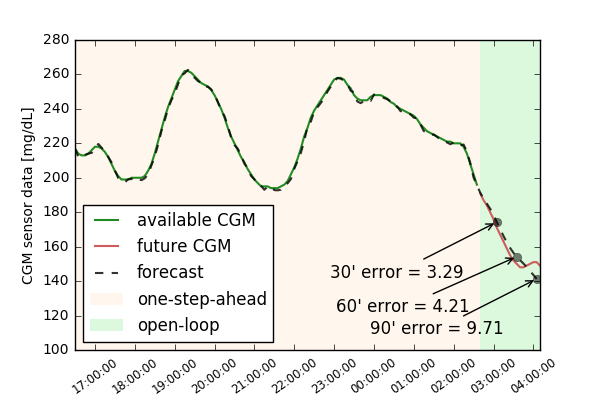
\includegraphics[width=0.8\textwidth]{part2/cgm_fit.png}
\end{figure}


\section{Conclusions and future works}

This chapter presented the last biomedical data science challenge of the thesis.

We compared the performance of two types of data-driven strategies for online CGM forecasting: recursive filters and ML models. We also illustrate a general procedure for model personalization based on cross-validation with hyperparameters optimization via grid-search.

Finally, we showed that reliable CGM predictions can be obtained with ML models that do not need to recursively adjust their parameters along time.
%In the next future we plan to investigate further using more advanced methods comprising deep learning approaches with  and sparse regularization methods.

In the future, to improve the performance on long prediction horizon, we plan to investigate sparse data representations with deeper architectures or regularized dictionary learning approaches.

\begin{table}[b!]
	\caption{Prediction errors (standard deviation) of the forecasting models for increasing prediction horizons, overall and on the four groups. {\sl MP} = Microinfusion Pump, {\sl II} = Insulin Injection, {\sl RAI} = Rapid Acting Insulin, {\sl Other} = Other therapies. Bold numbers indicate best result.}
	\label{tab:errors}
		\begin{tabular}{lllllll}
			& \multicolumn{6}{c}{ARIMA}                                              \\ \cline{2-7}
			\multicolumn{1}{l|}{}                           & \multicolumn{3}{c|}{MAE mg/dL}          & \multicolumn{3}{c|}{RMSE mg/dL}         \\ \cline{2-7}
			\multicolumn{1}{l|}{}                           & 30 & 60 & \multicolumn{1}{l|}{90} & 30 & 60 & \multicolumn{1}{l|}{90}  \\ \hline
			\multicolumn{1}{l|}{Overall}                    & 11.5 (5.2) & 25.6 (12.5) & \multicolumn{1}{l|}{37.2 (20.3)} & 16.7 (7.9) & 37.1 (19.3) & \multicolumn{1}{l|}{53.8 (31.8)} \\
			\multicolumn{1}{l|}{T1D - {\sl MP}}   & 13.3 (3.6) & 30.3 (7.4) & \multicolumn{1}{l|}{45.3 (12.5)} & 19.5 (5.4) & 43.9 (10.9) & \multicolumn{1}{l|}{64.9 (18.1)}  \\
			\multicolumn{1}{l|}{T1D - {\sl II}}    & 13.4 (6.3) & 31.0 (16.2) & \multicolumn{1}{l|}{46.1 (27.1)} & 19.7 (10.6) & 45.1 (27.0) & \multicolumn{1}{l|}{66.6 (45.7)}  \\
			\multicolumn{1}{l|}{T2D - {\sl RAI}} & {\bf11.0 (3.3)} & {\bf 23.8 (6.5)} & \multicolumn{1}{l|}{33.2 (8.5)} & 16.2 (4.8) & 34.1 (8.3) & \multicolumn{1}{l|}{46.9 (10.9)}  \\
			\multicolumn{1}{l|}{T2D - {\sl Other}}      & 10.0 (5.1) & 21.4 (10.4) & \multicolumn{1}{l|}{29.2 (12.5)} & 13.6 (6.0) & 29.6 (12.7) & \multicolumn{1}{l|}{41.3 (16.5)}  \\ \hline
			
			\\
			& \multicolumn{6}{c}{KF}                                                \\ \cline{2-7}
			\multicolumn{1}{l|}{}                           & \multicolumn{3}{c|}{MAE mg/dL}          & \multicolumn{3}{c|}{RMSE mg/dL}         \\ \cline{2-7}
			\multicolumn{1}{l|}{}                           & 30 & 60 & \multicolumn{1}{l|}{90} & 30 & 60 & \multicolumn{1}{l|}{90} \\ \hline
			\multicolumn{1}{l|}{Overall}              & 46.8 (23.2) & 50.8(25.4) & \multicolumn{1}{l|}{159.6 (43.5)} & 58.3 (27.7) & 63.1 (30.3) & \multicolumn{1}{l|}{169.9 (47.1)} \\
			\multicolumn{1}{l|}{T1D - {\sl MP}}         & 56.6 (15.9) & 59.5 (15.2) & \multicolumn{1}{l|}{163.5 (26.7)} & 70.5 (19.0) & 74.3 (18.4) & \multicolumn{1}{l|}{177.5 (29.9)} \\
			\multicolumn{1}{l|}{T1D - {\sl II}}    & 59.9 (24.5) & 67.9 (26.7) & \multicolumn{1}{l|}{179.2 (38.9)} & 74.4 (28.7) & 83.5 (31.3) & \multicolumn{1}{l|}{193.8 (40.4)} \\
			\multicolumn{1}{l|}{T2D - {\sl RAI}} & 48.6 (20.4) & 50.9 (20.8) & \multicolumn{1}{l|}{195.2 (63.1)} & 60.4 (22.9) & 63.6 (24.1) & \multicolumn{1}{l|}{204.4 (63.8)} \\
			\multicolumn{1}{l|}{T2D - {\sl Other}}      & 33.0 (12.1) & 35.6 (15.8) & \multicolumn{1}{l|}{145.0 (30.4)} & 41.3 (14.2) & 44.3 (17.7) & \multicolumn{1}{l|}{150.1 (31.8)} \\ \hline
			
			
			\\
			
			& \multicolumn{6}{c}{KRR}       \\ \cline{2-7}
			\multicolumn{1}{l|}{}                           & \multicolumn{3}{c|}{MAE mg/dL}          & \multicolumn{3}{c|}{RMSE mg/dL} \\ \cline{2-7}
			\multicolumn{1}{l|}{}                           & 30 & 60 & \multicolumn{1}{l|}{90} & 30 & 60 & \multicolumn{1}{l|}{90}  \\ \hline
			\multicolumn{1}{l|}{Overall}                    & {\bf 11.1 (4.3)} & {\bf 25.1 (10.4)} & \multicolumn{1}{l|}{{\bf 35.2 (15.4)}} & {\bf 15.5 (6.7)} & {\bf 33.6 (13.8)} & \multicolumn{1}{l|}{{\bf 45.8 (19.7)}} \\
			\multicolumn{1}{l|}{T1D - {\sl MP}}   & {\bf12.9 (3.4)} & {\bf 30.2 (8.4)} & \multicolumn{1}{l|}{{\bf 43.1 (12.6)}} & {\bf17.9 (5.1)} & {\bf 40.2 (10.9)} & \multicolumn{1}{l|}{{\bf 56.0 (16.1)}}  \\
			\multicolumn{1}{l|}{T1D - {\sl II}}    & {\bf13.1 (4.9)} & {\bf 30.3 (10.6)}  & \multicolumn{1}{l|}{{\bf 43.1 (14.5)}} & {\bf18.6 (8.4)} & {\bf 40.5 (14.5)} & \multicolumn{1}{l|}{{\bf 55.8 (18.6)}}  \\
			\multicolumn{1}{l|}{T2D - {\sl RAI}} & 11.2 (2.9) & 24.1 (5.5) & \multicolumn{1}{l|}{{\bf 33.2 (7.1)}} & {\bf16.0 (4.7)} & {\bf 32.7 (7.5)} & \multicolumn{1}{l|}{{\bf 43.7 (9.5)}}  \\
			\multicolumn{1}{l|}{T2D - {\sl Other}}      & {\bf8.7 (2.3)} & {\bf 19.8 (6.9)} & \multicolumn{1}{l|}{{\bf 27.7 (11.8)}} & {\bf11.9 (3.4)} & {\bf 26.5 (8.9)} & \multicolumn{1}{l|}{{\bf 36.2 (14.4)}}  \\ \hline
			
			\\
			
			& \multicolumn{6}{c}{LSTM}                                              \\ \cline{2-7}
			\multicolumn{1}{l|}{}                           & \multicolumn{3}{c|}{MAE mg/dL}          & \multicolumn{3}{c|}{RMSE mg/dL}         \\ \cline{2-7}
			\multicolumn{1}{l|}{}                           & 30 & 60 & \multicolumn{1}{l|}{90} & 30 & 60 & \multicolumn{1}{l|}{90} \\ \hline
			\multicolumn{1}{l|}{Overall}                & 19.9 (10.6) & 44.0 (25.9) & \multicolumn{1}{l|}{61.3 (36.5)} & 26.2 (13.4) & 55.0 (30.0) & \multicolumn{1}{l|}{74.7 (41.3)} \\
			\multicolumn{1}{l|}{T1D -{\sl  MP}}   & 22.9 (9.1) & 51.6 (21.5) & \multicolumn{1}{l|}{71.6 (27.0)} & 30.6 (11.6) & 65.7 (27.0) & \multicolumn{1}{l|}{89.8 (33.5)} \\
			\multicolumn{1}{l|}{T1D - {\sl II}}    & 24.5 (12.9) & 56.5 (33.1) & \multicolumn{1}{l|}{81.4 (45.8)} & 31.2 (14.9) & 68.8 (35.9) & \multicolumn{1}{l|}{97.0 (48.4)} \\
			\multicolumn{1}{l|}{T2D - {\sl RAI}} & 18.3 (6.7) & 39.4 (14.8) & \multicolumn{1}{l|}{54.1 (21.0)} & 25.7 (10.1) & 51.6 (21.7) & \multicolumn{1}{l|}{67.7 (29.1)} \\
			\multicolumn{1}{l|}{T2D - {\sl Other}}      & 16.8 (8.9) & 35.0 (17.7) & \multicolumn{1}{l|}{47.0 (26.5)} & 22.2 (12.1) & 43.4 (19.0) & \multicolumn{1}{l|}{56.5 (27.3)} \\ 
			
			\hline
			
		\end{tabular}
\end{table}



% !TEX root = ./main.tex

\chapter{Conclusions} \label{chap:conclusions}

Data science definition: \\
- hacking skills \\
- statistics \\
- domain knowledge \\

Machine learning definition: \\
- automating task with little human supervision \\
- solving complex problems \\
- model interpretability \\
- importance in clinic \\

The importance of data exploration: \\
- uncovering hidden structures \\
- insights on the collected data \\
- must be ran before supervised analysis \\
- it helps further steps \\

Molecular clock: \\
- description of the molecular biomarkers \\
- feature expansion \\
- sparsity eforcing linear model \\
- results \\

Multiple sclerosis: \\
- disease description \\
- pcos \\
- temporal model \\
- results \\

Diabetes: \\
- modern diabetes treatment \\
- temporal forecasting \\
- results \\





% Appendices
% !TEX root = ./main.tex
\appendix

\chapter{Appendix} \label{appendix:A}
As already pointed out at the beginning of Chapter~\ref{chap:state-of-the-art}, ML is a cross-disciplinary field and the statistical tools used in literature to describe models and algorithms heavily depend on the academic background of the author. This can make the approach to ML fascinating and somewhat cumbersome at the same time.

The goal of this appendix is to shed light on some of the statistical tools and definitions that are typically left unsaid, or given for granted, by most of the authors. In particular, in the following sections insightful statistical details on the formulation of the supervised learning problem expressed in Equation~\eqref{eq:losspen} will be provided.

%The expected value of the function $g(a,b)$, where $(a,b)$ are two continuous random variables with joint probability distribution $f(a,b)$, can be computed with the \textit{Law of the unconscious statistician} (\ac{LOTUS}), reported in Theorem~\ref{th:lotus}.

\section{Useful theorems and definitions}

This first section lists the theorems and the definitions that are useful for the comprehension of the following sections~\cite{keener2011theoretical, everitt2002cambridge}.

\begin{theorem}[Law of the unconscious statistician] \label{th:lotus}
	Given two continuous random variables $(a,b) \in A \times B$ with joint probability distribution $p(a,b)$, the expected value of the function $g(a,b)$ can be stated as follows.
	$$\mathbb{E}[g(a,b)]=\iint_{A \times B}g(a,b)~p(a,b)~dadb$$
\end{theorem}

\begin{definition}[Conditional probability] \label{th:pc}
	Given two events $A$ and $B$, the conditional probability of A given B is defined as
	$$ P(A|B) = \frac{P(A \cap B)}{P(B)} $$
	where $B$ is not an impossible event, \ie $P(B) > 0$.
%	if $A$ and $B$ are impossible events (\ie $P(A)=P(B)=0$), then $P(A|B) = 0$.
\end{definition}

\begin{theorem}[Bayes rule] \label{th:bayes_rule}
	Given $A$ and $B$ two events with probability $P(A)$ and $P(B) \neq 0$, the conditional probability of observing $A$ given that $B$ is true is
	$$P(A|B) = \frac{P(B|A) \cdot P(A)}{P(B)}$$
	where $P(B|A)$ is the probability of observing $B$ given that $A$ is true.
\end{theorem}

% \begin{theorem}[Chain rule] \label{th:chain_rule}
% 	Given $n$ events $A_1, A_2, \dots, A_n$ with probability $P(A_1), P(A_2), \dots, P(A_n)$ the joint probability $P(A_1, A_2, \dots, A_n)$ can be written as follows.
% 	$$P(A_1, A_2, \dots, A_n) = P(A_1|A_2, \dots, A_n) \cdot P(A_2|A_3, \dots, A_n) \dots P(A_{n-1}|A_{n}) \cdot P(A_n)$$
% \end{theorem}

\begin{definition}[Well-posed problem]
	A problem is \textbf{well-posed} if its solution:
	\begin{enumerate*}[label=(\roman*)]
		\item exists,
		\item is unique,
		\item depends continuously on the data (\eg it is stable).
	\end{enumerate*}
\end{definition}

\begin{definition}[Ill-posed problem] \label{def:ill_posed}
	A problem is \textbf{ill-posed} if it is not well-posed.
\end{definition}

\begin{definition}[Likelihood function] \label{def:likelihood}
	Let $\bm{a}$ be a continuous random variable with probability distribution $p(\bm{a}, \bm{\phi})$ depending on the parameter $\bm{\phi}$; then the function $\mathcal{L}(\bm{\phi}|\bm{\bar a})=p(\bm{\bar a},\bm{\phi})$ is the likelihood function of $\bm{\phi}$ given that $\bm{\bar a}$ is the outcome of $\bm{a}$.
	% Given the observed values $\bm{\bar a} = [\bar a_1, \bar a_2, \dots, \bar a_n]^T$, the likelihood function
	% % $$\mathcal{L}(\bm{\bar a}, \bm{\phi}) = p(\bm{\bar a}, \bm{\phi})$$
	% $p(\bm{\bar a}, \bm{\phi})$
	% and if the random variables $a_i$ (for $i=1,\dots,n$) are \text{\ac{iid}}, then the likelihood function can be simplified as follows.
	% $$\mathcal{L}(\bm{\bar a}, \bm{\phi}) = \prod_{i=1}^n p(\bar a_i, \bm{\phi})$$
\end{definition}


\section{Empirical risk minimization} \label{sec:erm}
In Section~\ref{subsec:supervised_learning} we introduced the concept of supervised learning as the branch of ML in which predictive models are trained on labeled data. The final goal of supervised learning is to find a function of the input variables $f: \mathcal{X} \rightarrow \mathcal{Y}$ that provides a \textit{good} approximation of the output $y$. In order to measure the adherence between predictions $\hat y = f(\bm{x})$ and actual output $y$, we introduced the concept of \textit{loss function} $L(\hat y, y)$, see Table~\ref{tab:losses}. For a fixed choice of the loss, the ideal estimator, also known as the \textit{target} function, $f^*$ is the minimizer of the (true) expected risk $\mathcal{E}(f)$ \ie
%in a rather \textit{large} class of functions $\mathcal{F}$.
%We assume that $f^*(\bm{x})$ minimizes $\mathbb{E}(f)$ in a rather \textit{large} class of functions $\mathcal{F}$.
\begin{equation} \label{eq:fstar}
	f^* = \argmin_{f \in \mathcal{F}_0}{\mathcal{E}(f)}
\end{equation}
where $\mathcal{F}_0$ is the (huge) class of functions $f: \mathcal{X} \rightarrow \mathcal{Y}$ such that $\mathcal{E}(f)$ is finite.

Applying the law of the unconscious statistician, stated in Theorem~\ref{th:lotus}, the expected risk $\mathcal{E}(f)$ can be written as in Equation~\eqref{eq:expected_loss}, where $(\bm{x},y)$ are two random variables with joint probability distribution $p(\bm{x},y)$.

\begin{equation} \label{eq:expected_loss}
	\mathcal{E}(f) = \mathbb{E}[L(f(\bm{x}),y)] = \iint_{\mathcal{X} \times \mathcal{Y}}L(f(\bm{x}),y)~p(\bm{x},y)~d\bm{x}dy
%	\mathcal{E}(f) = \mathbb{E}[L(f(\bm{x}),y))] = \int_{-\infty}^{+\infty}\int_{-\infty}^{+\infty} L(f(\bm{x}),y) p(\bm{x},y) d\bm{x}dy
\end{equation}

In real situations, a direct computation of $\mathcal{E}(f)$ is unfeasible as the joint probability distribution $p(\bm{x},y)$ is unknown. Although, we assume to be provided with a collection of input-output pairs $\mathcal{D}=\{(\bm{x}_i,y_i)\}_{i=1}^n$ that are supposed to be sampled \ac{iid} from $\mathcal{X} \times \mathcal{Y}$ according to $p(\bm{x}, y)$.
In statistical learning theory, as introduced by Vapnik~\cite{vapnik2013nature}, the dataset $\mathcal{D}$ can be used to build a stochastic approximation of $\mathcal{E}(f)$ called \textit{empirical risk} $\mathcal{E}_{\mathcal{D}}(f)$ and defined in Equation~\eqref{eq:empirical_risk}.

\begin{equation} \label{eq:empirical_risk}
	\mathcal{E}_{\mathcal{D}}(f) = \frac{1}{n} \sum_{i=1}^{n} L(f(\bm{x}_i), y_i)
\end{equation}

As $\mathcal{D}$ is drawn according to the probability distribution $p(\bm{x},y)$, our hope is that the empirical risk can be used as a proxy for the expected risk, hence $\mathcal{E}_{\mathcal{D}}(f) \approx \mathcal{E}(f)$. The solution of the supervised learning problem is then found by \textit{Empirical Risk Minimization} (ERM), defined in Equation~\eqref{eq:erm}

\begin{equation} \label{eq:erm}
	\hat f(\bm{x}) = \argmin_{f \in \mathcal{F}}{\mathcal{E}(f_{\mathcal{D}})} = \argmin_{f \in \mathcal{F}}{\frac{1}{n} \sum_{i=1}^{n} L(f(\bm{x}_i), y_i)}
\end{equation}

Where $\mathcal{F}$ is a suitable small subset of $\mathcal{F}_0$.
In practice, minimizing $\mathcal{E}(f_{\mathcal{D}})$ instead of $\mathcal{E}(f)$ comes at a price. The central problem is whether the first is a good approximation of the second. For instance, when $p(\bm{x}, y)$ is too \textit{complex}, the number of examples is too small and/or the class of functions $\mathcal{F}$ is \textit{too large}, $\hat f(\bm{x})$ will be far from the target function $f^*(\bm{x})$, even when its empirical error is $0$. In real circumstances, it is impossible to control the true probability distribution and it is often extremely difficult to collect a very large number of examples. The only element we can control is the class of functions $\mathcal{F}$ and, in particular, its \textit{size}. Since Tikhonov~\cite{tikhonov1963solution} it is known that, for an arbitrary function space $\mathcal{F}$, the ERM problem is ill-posed (see Definition~\ref{def:ill_posed}). A possible way to ensure well-posedness is to impose a constrain that restricts the function space. Hence, the constrained ERM problem assumes the form in Equation~\eqref{eq:constrained_erm}, where $\lambda \neq 0$.

\begin{equation} \label{eq:constrained_erm}
	\begin{aligned}
		\argmin_{f \in \mathcal{F}}{\frac{1}{n} \sum_{i=1}^{n} L(f(\bm{x}_i), y_i)} \\
		\text{subject to}~\mathcal{R}(f) < \frac{1}{\lambda}
	\end{aligned}
\end{equation}

Applying the \textit{Lagrange multipliers technique}\footnote{ For a thorough description of this technique, see Appendix E of Bishop's book~\cite{bishop2006pattern}.} Equation~\eqref{eq:constrained_erm} can be finally written as Equation~\eqref{eq:losspen2}.

\begin{equation} \label{eq:losspen2}
	\argmin_{f \in \mathcal{F}}{\frac{1}{n} \sum_{i=1}^{n} L(f(\bm{x}_i), y_i)} + \lambda \mathcal{R}(f)
\end{equation}

The penalty term $\mathcal{R}(f)$ acts as regularizer \footnote{ $\mathcal{R}(f)$, in general, can be thought as $\mathcal{R}(f) = \norm{f}^2_K$ where $\norm{\cdot}^2_K$ is the norm defined by the kernel $K$ in a \textit{Reproducing Kernel Hilbert Space} $\mathcal{H}$~\cite{evgeniou2000regularization, vito2005learning}.}
and, according to its definition, it can ensure well-posedness of the problem and it can enforce different interesting properties on the achieved solution, see Section~\ref{subsec:regularization_methods}. It can also be shown that the use of appropriate regularizes promotes generalization, hence increases our chance to find a $\hat f(\bm{x})$ \textit{close} to $f^*(\bm{x})$.

 According to the choice made for $L(\cdot)$ and $\mathcal{R}(\cdot)$, the minimization problem posed in Equation~\eqref{eq:losspen2} can have very different properties; it can be convex or non-convex, it can include differentiable as well as non-differentiable terms. A rigorous review of the most common optimization methods for ML is beyond the scope of this thesis and can be found here~\cite{boyd2004convex, vito2005learning, bach2012optimization, sra2012optimization, nesterov2013introductory}.


\section{Maximum likelihood  estimation} \label{sec:mle}
In this section we will see a different approach to tackle the supervised learning problem.
Once again, let the training data be made of input-output pairs $\mathcal{D} = \{(\bm{x}_i, y_i)\}_{i=1}^n$, with $(\bm{x}_i,y_i) \in \mathcal{X} \times \mathcal{Y}$, $\forall~i=1,\dots,n$. This approach relies on the expression of the uncertainty over the value of $y$ with a probability distribution $p(y|\bm{x},\bm{\theta})$ parameterized by $\bm{\theta} \in \Theta$.
Applying Definition~\ref{def:likelihood}, and assuming that the samples are drawn \ac{iid}, we can write the likelihood function for $\bm{\theta}$ as in Equation~\eqref{eq:likelihood}.

\begin{equation} \label{eq:likelihood}
	\mathcal{L}(y|\bm{x}, \bm{\theta}) = \prod_{i=1}^{n} p(y_i | \bm{x}_i , \bm{\theta})
\end{equation}

Equation~\eqref{eq:likelihood} can be considered as the probability of observing the output $y_i$, given the input $\bm{x}_i$ and the parameters $\bm{\theta}$ ($\forall i=1,\dots,n$).
This statistical setup suggests a strategy to obtain an estimate for $\bm{\theta}$ known as \textit{Maximum Likelihood Estimation} (MLE), see Equation~\eqref{eq:mle}.

\begin{equation} \label{eq:mle}
	\bm{\hat \theta}_{MLE} =\argmax_{\theta~\in~\Theta}\mathcal{L}(y_i|\bm{x}_i, \bm{\theta}) = \argmax_{\theta~\in~\Theta} \prod_{i=1}^{n} p(y_i | \bm{x}_i, \bm{\theta})
\end{equation}

Instead of maximizing the likelihood it is often convenient to minimize the \textit{negative log-likelihood}\footnote{ Approaching information theory or deep learning literature, the negative log-likelihood is often referred to as \textit{cross-entropy}.}. Equation~\eqref{eq:mle} can then be rewritten as Equation~\eqref{eq:nll}.

\begin{equation} \label{eq:nll}
	\bm{\hat \theta}_{MLE} = \argmin_{\theta~\in~\Theta} - \sum_{i=1}^n \log p(y_i | \bm{x}_i, \bm{\theta})
\end{equation}

Moreover, if some prior knowledge on $\bm{\theta}$ is available, it is possible to incorporate it in the form of a prior distribution $p(\bm{\theta})$. Applying the Bayes rule (Theorem~\ref{th:bayes_rule}) it is possible to write the \textit{posterior distribution} $p(\bm{\theta}|y,\bm{x})$ as in Equation~\eqref{eq:posterior}.

\begin{equation} \label{eq:posterior}
	p(\bm{\theta}|y,\bm{x}) = \frac{p(y|\bm{x}, \bm{\theta}) \cdot p(\bm{\theta})}{p(y|\bm{x})}
\end{equation}

The normalizing constant in Equation~\eqref{eq:posterior} $p(y|\bm{x})$ is independent from $\bm{\theta}$. It is known as the marginal likelihood and it can be estimated as in Equation~\eqref{eq:marginal_likelihood}.

\begin{equation} \label{eq:marginal_likelihood}
	p(y|\bm{x}) = \int p(y|\bm{x}, \bm{\theta}) \cdot p(\bm{\theta})~d\bm{\theta}
\end{equation}

Equation~\eqref{eq:posterior} suggest a new strategy to achieve an estimate for $\bm{\theta}$ that takes into account the prior distribution. This criterion is stated in Equation~\eqref{eq:map} and it is known as \textit{Maximum A Posteriori} (MAP).

\begin{equation} \label{eq:map}
	\bm{\hat \theta}_{MAP} = \argmax_{\theta~\in~\Theta} p(\bm{\theta}|y,\bm{x}) = \argmax_{\theta~\in~\Theta} p(y|\bm{x}, \bm{\theta}) \cdot p(\bm{\theta})
\end{equation}

Finally, given that $p(y|\bm{x}, \bm{\theta})$ is the likelihood of $\bm{\theta}$ (see Definition~\ref{def:likelihood}), we can assume \ac{iid} samples and apply the negative log-likelihood trick to rewrite Equation~\eqref{eq:map} as in Equation~\eqref{eq:map2}.

\begin{equation} \label{eq:map2}
	\bm{\hat \theta}_{MAP} = \argmin_{\theta~\in~\Theta} - \bigg[\sum_{i=1}^n \log p(y_i|\bm{x}_i,\bm{\theta})  + \log p(\bm{\theta})\bigg]
\end{equation}

Fixing the two distributions, the predictive model can be achieved solving the minimization problem in Equation~\eqref{eq:map2}. For the solution of this minimization problem the same observations provided at the end of the last section for Equation~\eqref{eq:losspen2} hold.

\section{ERM vs MLE/MAP} \label{sec:erm-mlemap_connection}
The goal of this last section is to show that the approaches described in Section~\ref{sec:erm} and in Section~\ref{sec:mle} look very different, but they actually are two sides of the same coin.

Assuming that we have the usual collection of \ac{iid} samples $\mathcal{D}=\{(\bm{x}_i,y_i)\}_{i=1}^n$, where $(\bm{x}_i,y_i) \in \mathcal{X} \times \mathcal{Y}~\forall~i=1,\dots,n$, our aim here is to learn a good input-output relationship $f: \mathcal{X} \rightarrow \mathcal{Y}$. The function $f$ may depend from some parameters that, for ease of writing, will be temporary omitted. If we decide to proceed by MLE, we can find $\hat f_{MLE}$ solving the optimization problem in Equation~\eqref{eq:fmle}.

\begin{equation} \label{eq:fmle}
	\hat f_{MLE} = \argmax_{f~\in~\mathcal{F}} \prod_{i=1}^n p(y_i|\bm{x}_i,f)
\end{equation}

Applying the negative log-likelihood trick, Equation~\eqref{eq:fmle} can be rewritten as Equation~\eqref{eq:logfmle}.
%\footnote{ The two minimization problems $\min_x f(x)$ and $\min_x \alpha f(x)$ have the same solution if $\alpha$ is a constant that does not depend from $x$.}.

\begin{equation} \label{eq:logfmle}
	\hat f_{MLE} = \argmin_{f~\in~\mathcal{F}} - \frac{1}{n} \sum_{i=1}^n \log p(y_i|\bm{x}_i,f)
\end{equation}

As we can see here, we are naming \textit{negative log-likelihood} what in Section~\ref{sec:erm} was called \textit{loss function}. In fact, using $L(f(\bm{x}), y) = -\log p(y|\bm{x}, f)$ Equation~\eqref{eq:logfmle} can be rewritten as in Equation~\eqref{eq:ferm}, which is the ERM problem.

\begin{equation} \label{eq:ferm}
	\hat f_{ERM} = \argmin_{f~\in~\mathcal{F}} \frac{1}{n} \sum_{i=1}^n L(f(\bm{x}_i), y_i)
\end{equation}

In Section~\ref{sec:erm} we have seen that introducing $\mathcal{R}(f)$ reduces the space of functions $\mathcal{F}$ and prevents the achieved solution from overfitting. Intuitively, the same effect can be achieved by introducing a prior $p(f)$ as in the MAP estimate. Following Equation~\eqref{eq:map2} we can write Equation~\eqref{eq:map3}.

\begin{equation} \label{eq:map3}
	\hat f_{MAP} = \argmin_{f~\in~\mathcal{F}} - \frac{1}{n} \bigg[ \sum_{i=1}^n \log p(y_i|\bm{x}_i,f) + \lambda \log p(f) \bigg]
\end{equation}

Finally, as for Equation~\eqref{eq:ferm}, we can express the penalty as $R(f) = - \frac{\lambda}{n} \log p(f)$ and Equation~\eqref{eq:map3} becomes Equation~\eqref{eq:ferm2}, which is the classical $Loss + Penalty$ formulation of the ERM problem.

\begin{equation} \label{eq:ferm2}
	\hat f_{ERM} = \argmin_{f~\in~\mathcal{F}} \frac{1}{n} \sum_{i=1}^n L(f(\bm{x}_i), y_i) + \lambda R(f)
\end{equation}

In this section an intuitive explanation of the connection between two popular supervised learning approaches is provided. For a more rigorous overview on ERM and MLE/MAP we refer to~\cite{hastie2009elements} and to~\cite{rasmussen2006gaussian}, respectively.

\subsection{Linear regression revisited} \label{subsec:linear_regression_revisited}

To clarify the connection between ERM and MLE/MAP we can revisit the simple linear regression problem.

Once again, we have a collection of \ac{iid} samples $\mathcal{D}=\{(\bm{x}_i,y_i)\}_{i=1}^n = (X, \bm{y})$, where $(\bm{x}_i,y_i) \in \mathcal{X} \times \mathcal{Y}$ $\forall~i=1,\dots,n$ and our aim is to learn an input-output relationship $f: \mathcal{X} \rightarrow \mathcal{Y}$.
Moreover, we assume that the outputs $y_i$ is affected by additive Gaussian noise, hence $y_i = f(\bm{x}_i) + \varepsilon$ where $\varepsilon \sim \mathcal{N}(0,\sigma_n^2)$.
Interestingly, this corresponds to the assumption that $f$ is modeling the mean of the outputs $y_i$, while its standard deviation $\sigma_n$ remains unknown, therefore $y_i \sim \mathcal{N}(f(\bm{x}_i), \sigma_n^2)$ ($\forall~i=1,\dots,n$).
In Section~\ref{sec:erm} we have seen that the ERM solution can be estimated as in Equation~\ref{eq:ferm}. For the sake of simplicity we can restrict to the Ridge Regression  case (see Section~\ref{subsec:regularization_methods}), \ie we look for a model that can be written as $\hat y = f(\bm{x}) = \bm{x}^T \bm{ \hat w}$ minimizing the square loss $L(\hat y,y) = \frac{1}{n} \norm{y - X\bm{w}}_2^2$ penalized by the $\ell_2$-norm $\mathcal{R}(\bm{w}) = \norm{w}_2^2$.
Therefore, the minimization problem is stated in Equation~\eqref{eq:ridge_regression2}.

\begin{equation} \label{eq:ridge_regression2}
	\bm{\hat w}_{\ell_2} = \argmin_{\bm{\hat w} \in \mathbb{R}^d} J(\bm{y}, X, \bm{w}) = \argmin_{\bm{\hat w} \in \mathbb{R}^d}\frac{1}{2n} \norm{\bm{y} - X\bm{w}}_2^2+\frac{\lambda}{2}\norm{\bm{w}}_2^2
\end{equation}

In Section~\ref{sec:erm-mlemap_connection} we have seen that the regularized minimization problem corresponds to a MAP estimate with an appropriate choice for negative log-likelihood and prior distribution (on $\bm{w}$) which correspond to loss function and regularization penalty, respectively. So, considering $J(\bm{y}, X, \bm{w})$ as a negative log-posterior and factoring out $\lambda$ we can write
$$
\exp{\bigg[-J(\bm{y}, X, \bm{w})\bigg]} \propto \exp \bigg[ -\frac{1}{2n\lambda} \norm{\bm{y}-X\bm{w}}_2^2 \bigg] \cdot \exp{\bigg[-\frac{1}{2}\norm{w}_2^2 \bigg]}
$$
which can be seen as
$$
p(\bm{w}|\bm{y},X) = p(\bm{y}|X,\bm{w}) \cdot p(\bm{w})
$$
where $p(\bm{y}|X,\bm{w}) = \mathcal{N}(X\bm{w},n \lambda I)$ and $p(\bm{w}) = \mathcal{N}(0,I)$. So, in this probabilistic interpretation, the variance of the noise affecting the output $\bm{y}$ plays the role of the regularization parameter $\lambda \approx \sigma_n^2$.


% The likelihood for the weights $\bm{w}$ of the linear model can be written as in Equation~\eqref{eq:gaussian_likelihood}.
%
% \begin{equation} \label{eq:gaussian_likelihood}
% 	\mathcal{L}(\bm{y}|X, \bm{w}) = \prod_{i=1}^n p(y_i|\bm{x}_i, \bm{w}) = \prod_{i=1}^n \frac{1}{\sqrt{2\pi}\sigma} \exp \bigg[ -\frac{(y_i-\bm{x}_i^T\bm{w})^2}{2\sigma^2} \bigg] = \mathcal{N}(X^T\bm{w}, \sigma_n^2I)
% \end{equation}
%
% Moreover, as a measure against overfitting, we assume a zero mean Gaussian prior with covariance $\Sigma_p$ over the weights $\bm{w} \sim \mathcal{N}(0,\Sigma_p)$.
% Omitting the terms that do not depend from $\bm{w}$, we can write the posterior distribution as in Equation~\ref{eq:posterior_f}.
%
% \begin{equation} \label{eq:posterior_f}
% 	p(\bm{w}|X, y) \propto \exp \big[ -\frac{1}{2\sigma_n^2} (\bm{y}-X^T\bm{w})^T(\bm{y}-X^T\bm{w}) \big] \exp \big[ -\frac{1}{2} \bm{w}^T \Sigma_p^{-1} \bm{w} \big]
% \end{equation}
%
% With some elementary linear algebra operations it is possible to recognize that the Gaussian posterior distribution $p(\bm{w}|X, y) \sim \mathcal{N}(\bm{\bar w}, A^{-1})$, where $\bm{\bar w} = \frac{1}{\sigma_n^2}(\frac{1}{\sigma_n^2} XX^T+\Sigma_p^{-1})^{-1}X\bm{y}$ and $A = \frac{1}{\sigma_n^2} XX^T + \Sigma_p^{-1}$.


\subsection{Logistic regression revisited} \label{subsec:logistic_regression_revisited}

In this section we revisit binary classification via logistic regression from a probabilistic perspective.

In binary classification problems we are provided with a collection of input-output pairs $\mathcal{D}=\{(\bm{x}_i, y_i)\}_{i=1}^n = (X, \bm{y})$, where $\bm{x}_i \in \mathcal{X}$ and $y_i \in \{+1,-1\}$, $\forall i=1,\dots,n$.
Once again we are looking for a model $f: \mathcal{X} \rightarrow \mathcal{Y}$ that associates each input sample with its corresponding class. For the sake of simplicity we restrict to the case of linear functions $\hat y = f(\bm{x}) = \bm{x}^T\bm{\hat w}$.

The main idea behind logistic regression is to use a loss function having a $[0,1]$ range to estimate the probability that a sample $\bm{x}_i$ belongs to one of the two classes. As suggested by its name, the function of choice is the logistic $\sigma(z) = [1+\exp{(-z)}]^{-1}$.

In this context, we model our outputs $y_i$ as Bernoulli random variables, which implies that
$$
P(y=1 | \bm{x}) = \sigma(-f(\bm{x})) = \frac{1}{1+\exp{(-f(\bm{x}))}}
$$
and
$$
P(y=-1 | \bm{x}) = \sigma(f(\bm{x})) = \frac{1}{1+\exp{(f(\bm{x}))}}
$$
consequently, we can write the general form as in Equation~\eqref{eq:logistic}.

\begin{equation} \label{eq:logistic}
	P(y = \pm 1 | \bm{x}) = \frac{1}{1+\exp{(-y f(\bm{x}))}}
\end{equation}

Therefore, assuming a Gaussian prior on the weights $\bm{w} \sim \mathcal{N}(0,I)$, we can perform a MAP estimate of $\hat f$ solving the problem in Equation~\eqref{eq:logistic_map}.

\begin{equation} \label{eq:logistic_map}
	\bm{\hat w}_{\text{LR}} = \argmax_{\bm{\hat w} \in \mathbb{R}^d} \prod_{i=1}^n p(\bm{w}|y_i, \bm{x}_i) = \argmax_{\bm{\hat w} \in \mathbb{R}^d} \prod_{i=1}^n \frac{1}{1+\exp{(-y_i~\bm{x}_i^T\bm{w})}} \cdot \exp{(-\frac{1}{2} \norm{\bm{w}}_2^2)}
\end{equation}

Log-transforming Equation~\eqref{eq:logistic_map}, and applying some elementary linear algebra, we can write Equation~\eqref{eq:logistic_logmap}.

\begin{equation} \label{eq:logistic_logmap}
	\bm{\hat w}_{\text{LR}} = \argmin_{\bm{\hat w} \in \mathbb{R}^d} \frac{1}{2n\lambda} \sum_{i=1}^n \log \big[ 1 + \exp{(-y_i \bm{x}_i^T \bm{w})} \big] + \frac{\lambda}{2} \norm{\bm{w}}_2^2
\end{equation}

The minimization problem expressed in Equation~\eqref{eq:logistic_logmap} is known as Regularized Logistic Regression. It can be casted in the regularization framework of Equation~\eqref{eq:ferm2} where the logistic loss function $L(f(\bm{x}),y) = \log{[1+\exp{(-yf(\bm{x}))}]}$ is penalized by the $\ell_2$-norm.









% asd\footnote{ In the deep learning literature this is usually named \textit{activation} function.}
%%


% LIST OF STUFF
\backmatter
\listoffigures
\listoftables
\newpage
\printacronyms[include-classes=abbrev,name=List of Abbreviations]
%\newpage
%\printacronyms[include-classes=nomencl,name=Nomenclature]
\newpage

\cleardoublepage
% \bibliographystyle{alpha}   % <-- default
\bibliographystyle{apalike} % <-- but I like this one more
% \bibliographystyle{plain}     % <-- good for draft
\bibliography{biblio}


\end{document}
